\documentclass[french,12pt,twoside,a4paper]{book}
\usepackage[margin=2.3cm]{geometry}

% headers and typo stuffs
\usepackage{fancyhdr}
\usepackage{array}
\usepackage{multirow} %% Pour mettre un texte sur plusieurs rangées
\usepackage{multicol} %% Pour mettre un texte sur plusieurs colonnes
\usepackage{scrextend} %Forcer la 4eme  de couverture en page pair
\usepackage[utf8]{inputenc}
\usepackage[T1]{fontenc}
\usepackage{titlesec} % change titles formatting
\usepackage{tocloft} %% toc formatting
%\usepackage[french]{babel} % deactivating french babel that yields an error
%\usepackage{csquotes} % for csquotes not present in babel french
\usepackage[absolute]{textpos} 
\usepackage{lipsum}
% fonts
\usepackage{lmodern}
%---------------------------------------------------------
% Semi-bold condensed. Works only with lmodern
\def\sbc{\sffamily\fontseries{sbc}\selectfont}

\setlength{\textwidth}{\dimexpr\paperwidth-2.3cm-2.3cm\relax}
\setlength{\marginparsep}{.85cm}
\setlength{\marginparwidth}{3.4cm}

% links and url
\usepackage{hyperref}       % hyperlinks
\usepackage{url}            % simple URL typesetting
\hypersetup{%pdftex,  % needed for pdflatex
  breaklinks=true,  % so long urls are correctly broken across lines
  colorlinks=true,
  urlcolor=deep_brown,
  linkcolor=deep_blue,
  citecolor=dark_green,
  }

  \usepackage{enumitem}
  \setlist[itemize]{label=\textcolor{ared}{\rule{1ex}{1ex}}}
  \setlist[description]{font=\bfseries\sffamily}
  \setlist[enumerate]{font=\bfseries\sffamily\color{ared}}
  
  
% figures
\usepackage{graphicx}
\usepackage{caption}
\usepackage{subcaption}
\usepackage{placeins}
% tables
\usepackage{booktabs} % professional-quality tables
\usepackage{tabularx}
\usepackage{colortbl}
\usepackage{threeparttable}
\usepackage{multirow}
\usepackage{makecell}
\usepackage[right]{lineno}
\usepackage[nopatch=eqnum]{microtype}
\usepackage{lscape}
% Define some commands for table
\newcolumntype{+}{!{\vrule width 2pt}}
% create \thickcline for thick horizontal lines of variable length
\newlength\savedwidth \newcommand\thickcline[1]{%
  \noalign{\global\savedwidth\arrayrulewidth\global\arrayrulewidth 2pt}%
  \cline{#1}%
  \noalign{\vskip\arrayrulewidth}%
  \noalign{\global\arrayrulewidth\savedwidth}%
}
% \thickhline command for thick horizontal lines that span the table
\newcommand\thickhline{\noalign{\global\savedwidth\arrayrulewidth\global\arrayrulewidth
2pt}%
\hline
\noalign{\global\arrayrulewidth\savedwidth}}


% csv
\usepackage{csvsimple}
% maths
\usepackage{amsfonts}  % blackboard math symbols
\usepackage{amsmath}
\usepackage{amssymb} %mathbb packages

\usepackage{siunitx}
\usepackage{algorithm, algorithmicx, algpseudocode}
% TODO: test if not happy with current algo styling
%\usepackage[ruled, linesnumbered, fillcomment]{algorithm2e}

% color commands
\usepackage[dvipsnames]{xcolor} % colors
\colorlet{P}{ForestGreen}
\colorlet{I}{MidnightBlue}
\colorlet{C}{YellowOrange}
\colorlet{O}{DarkOrchid}
\definecolor{Prune}{RGB}{99,0,60}
\definecolor{light_grey}{rgb}{0.3,.3,.3}
\definecolor{deep_blue}{rgb}{0,.2,.5}
\definecolor{dark_blue}{rgb}{0,.15,.5}
% Less saturation in the green for citations
\definecolor{dark_green}{rgb}{0.2,0.5,.3}
%\definecolor{dark_green}{rgb}{0,0.5,.15}
\definecolor{firebrick}{rgb}{0.75,0.125,0.125}
\definecolor{indigo}{rgb}{0.3,0,0.5}
% Color from http://paletton.com/#uid=30v0u0kllllaFw0g0qFqFg0w0aF
\definecolor{dark_brown}{RGB}{85, 39, 0}
\definecolor{deep_brown}{RGB}{128, 70, 21}
\definecolor{lightgreen}{RGB}{138,255,138}
\definecolor{lightblue}{RGB}{138,138,255}
\definecolor{ared}{rgb}{.647,.129,.149}
\colorlet{deep_color}{deep_blue}
\colorlet{dark_color}{dark_blue}
\definecolor{lightorange}{RGB}{255,212,138}
\colorlet{background_info_color}{green!10!orange}

\colorlet{chaptercolor}{deep_blue}
 % strange need to upper case for section numbering
\colorlet{CHAPTERCOLOR}{chaptercolor}
\colorlet{GRAY}{Gray}

% bibliography
\usepackage[natbib=true,style=authoryear,maxnames=999,maxcitenames=2,backend=biber]{biblatex}
% separators for bib
\DeclareDelimFormat{finalnamedelim}{\addsemicolon\space}
\DeclareDelimFormat[bib]{nametitledelim}{\addcolon\space}
\DeclareDelimFormat[bib]{titleyeardelim}{\addcomma\space}
% color for citations
\DeclareFieldFormat{biblabelnumber}{\textcolor{dark_green}{#1}}
% small bibliography
\DeclareFieldFormat{bibfont}{\footnotesize\sloppy #1}
\addbibresource{references.bib}

% appendix
\usepackage[toc,titletoc,page]{appendix}

% notes in the margin
\usepackage{todonotes}
\usepackage{snaptodo}

% comments
\snaptodoset{block rise=1em}
\snaptodoset{margin block/.style={font=\tiny}} \newcommand{\gv}[1]{%
  \snaptodo[margin block/.append style=green!50!black]{%
    \sloppy\textbf{Gael}: #1}}
\snaptodoset{margin block/.style={font=\tiny}} \newcommand{\md}[1]{%
  \snaptodo[margin block/.append style=blue]{%
    \sloppy\textbf{Matthieu}: #1}}

%%%%%%% boxes %%%%%%%%
\usepackage{tikz}
\usepackage{mdframed}
\usepackage[skins]{tcolorbox}

% Define a new box environment lefthandside background information box
\tcbuselibrary{breakable}
\tcbset{%
  mytitle/.style={%
      enhanced,
      overlay={
          \node [rotate=90, anchor=south, fill=tcbcolframe!25] at (frame.west) {\itshape \scriptsize #1};
        },
    },
  rightrule=0pt,
  skin=enhanced,parbox=false,breakable
}
\newtcolorbox{background_box_left}[1][]{
  mytitle=\textcolor{background_info_color}{Background Information},
  %title style={flushright},
  colframe=background_info_color, enhanced, colback=white, frame hidden, enlarge
  left by=-1cm,boxsep=0mm, left=1cm, borderline west =
    {2pt}{0pt}{background_info_color}, #1 }

% Define a new box environment for citations
\newenvironment{citationbox}{
  %\def\boxcontent{#1}%
  \begin{tcolorbox}[
      enhanced,
      colback=gray!10, % Background color of the box (gray with 10% intensity)
      colframe=white, % Border color of the box (white)
      arc=0mm, % Roundness of the corners (0mm means sharp corners)
      boxrule=0.5pt, % Border width (adjust as needed)
      rightrule=0pt, % Right border width (0pt for no border on the right side)
      %enlarge left by=8cm,
      left=0pt, % Left margin (0pt means no extra margin on the left)
      right=0pt, % Right margin (0pt means no extra margin on the right)
      top=0pt, % Top margin (0pt means no extra margin on the top)
      bottom=0pt, % Bottom margin (0pt means no extra margin on the bottom)
      rightupper=0mm, % Extra space on the right side for the citation
      rightlower=0mm, % Extra space on the right side for the citation
      %halign=flush right, % Text alignment within the box (right-aligned)
      width=0.9\textwidth,
      flush right,
      ]
    \footnotesize % Set the font size to script size
    \itshape % Make the text content italic
    }{
  \end{tcolorbox}%
  %\textcolorbox{\boxcolor}{\textit{\boxcontent}}
}
%Handling Keywords
\def\keywordname{{\bfseries \emph Keywords}}%
\def\keywords#1{\par\addvspace\medskipamount{\rightskip=0pt plus1cm
    \def\and{\ifhmode\unskip\nobreak\fi\ $\cdot$
    }\noindent\keywordname\enspace\ignorespaces#1\par}}

% 
\newenvironment{chapterabstract}{%
    \par\nobreak\noindent
    \textbf{\textit{Chapter's content}\hrulefill}\par\nobreak
    \small
    \noindent\ignorespaces
  }{%
    \par\nobreak\normalsize
    \vskip-\ht\strutbox\noindent
    \textbf{\hrulefill}%
}
% equations commands
\newcommand{\indep}{\perp \!\!\! \perp}
\newtheorem{assumption}{Assumption}
\newtheorem{definition}{Definition}
\newtheorem{proposition}{Proposition}
\newtheorem{proposition*}{Proposition}
\newtheorem{lemma}{Lemma}
\newtheorem{proof}{Proof}

\DeclareMathOperator*{\argmin}{argmin} \def\mycitecolor{green!50!black}
\usepackage{mathtools}
\newcommand\myeq{\stackrel{\mathclap{\text{def}}}{=}}

%%%%%%%%%%%%% Styling for contents (chapter, title, caption, ...) %%%%%%%%%%%%

% Styling of section numbering to have the chapter number hang
% The color of the chapter number outside of the section titles
% The font of section numbers in titles
\let\fontnumber\relax

% Section fonts
% chapter color


\titleformat{\chapter}[display]
  {\normalfont\Huge\bfseries\color{ared}}
  {\hfill \chaptertitlename\ \thechapter}
  {20pt}
  {\Huge\itshape\filleft}
\titlespacing*{\chapter}{0pt}{0pt}{20pt}  

\titleformat{\section}
  {\Large\bfseries\sffamily}
  {\thesection}
  {1em}
  {}

\titleformat{\subsection}
  {\large\bfseries\sffamily}
  {\thesubsection}
  {1em}
  {}

\titleformat{\subsubsection}
  {\bfseries\sffamily}
  {\thesubsubsection}
  {1em}
  {}

\titleformat{\paragraph}
  {\bfseries}
  {}
  {0em}
  {}

\titleformat{\subparagraph}
  {\sffamily\bfseries}
  {}
  {0em}
  {}

% The caption

\DeclareCaptionFont{captionnamefont}{\small\sffamily\color{MidnightBlue}}
\DeclareCaptionFont{captiontitlefont}{\small\sffamily}

\captionsetup{
  font={captionnamefont,captiontitlefont},
  labelfont=bf,
  labelsep=period,
  format=plain,
  figurename=Fig.
}

% ------------------------------------------------------------------
% Table of content
\setcounter{tocdepth}{2}
\renewcommand{\cftchapfont}{\bfseries\sffamily}
\renewcommand{\cftsecfont}{\sffamily}
\renewcommand{\cftsubsecfont}{\small\sffamily}


% headers
\usepackage{lastpage}
\usepackage{textcase}

\fancypagestyle{basic}{%
  \fancyhf{} % Clear header and footer
  \fancyhead[R]{\small \sffamily \nouppercase{\rightmark}} % Display subsections in the head
  %\fancyhead{\scriptsize \sffamily\rightmark} % Clear header
  \fancyfoot[C]{} % Centered footer
  \fancyfoot[R]{\small\sffamily M. Doutreligne} % Right footer
  \fancyfoot[L]{\small \thepage\,/\,\protect\pageref*{LastPage}} % Left footer
}

% renew section numbering
% Redefine the format for section numbers in the Table of Contents
\renewcommand{\thesection}{\fontnumber{\color{Gray}\arabic{chapter}.}\arabic{section}}
\renewcommand{\thesubsection}{\fontnumber{\color{Gray}\arabic{chapter}.}\arabic{section}.\arabic{subsection}}

% ------------------------------------------------------------------
% The title page
\newlength{\drop}%
\setlength{\drop}{2cm}%
\makeatletter%
\renewcommand*{\maketitle}{\begingroup%
  \thispagestyle{empty}%
  \raggedleft%
  \vspace*{\baselineskip}
  \textcolor{ared}{\LARGE\bfseries\sffamily \@title}%
  %\vfill%
  \\[0.067\textheight]%
  \sffamily\Large\@author
  %\\[\baselineskip]
  \vfill
  %{\Large The Publisher}\par%\plogo}\par
  %\vspace*{3\baselineskip}%
  \endgroup}
\makeatother%


% ------------------------------------------------------------------
% The styling of the abstract
\newenvironment{abstract}
{%
  \hfill%
  \begin{minipage}{.8\linewidth}\rmfamily\small
    \hrule\vspace*{.5ex}
    }
    {%
    \hrule%
  \end{minipage}%
  \vfill
}



\begin{document}
\frontmatter

%%%%%%%% TITLE PAGE %%%%%%%
\begin{titlepage}


  %\thispagestyle{empty}

  \newgeometry{left=6cm,bottom=2cm, top=1cm, right=1cm}

  \tikz[remember picture,overlay] \node[opacity=1,inner sep=0pt] at (-13mm,-135mm){
\includegraphics{img/Bandeau_UPaS.pdf}};

  % fonte sans empattement pour la page de titre
  \fontfamily{fvs}\fontseries{m}\selectfont


  %*****************************************************
  %******** NUMÉRO D'ORDRE DE LA THÈSE À COMPLÉTER *****
  %******** POUR LE SECOND DÉPOT                   *****
  %*****************************************************

  \color{white}

  \begin{picture}(0,0)

    \put(-110,-743){\rotatebox{90}{NNT: 2020UPASA000}}
  \end{picture}

  %*****************************************************
  %**  LOGO  ÉTABLISSEMENT PARTENAIRE SI COTUTELLE
  %**  CHANGER L'IMAGE PAR DÉFAUT **
  %*****************************************************
  \vspace{-10mm} % à ajuster en fonction de la hauteur du logo
  \flushright 
\includegraphics[scale=1]{img/logo2.png}




  %*****************************************************
  %******************** TITRE **************************
  %*****************************************************
  \flushright
  \vspace{10mm} % à régler éventuellement
  \color{Prune}
  \fontfamily{cmss}\fontseries{m}\fontsize{22}{26}\selectfont
  Représentations et
  inférence à partir de données de santé temporelles collectées en routine

  \normalsize
  \color{black}
  \Large{\textit{Representations and inference from time-varying routine care data}}
  %*****************************************************

  %\fontfamily{fvs}\fontseries{m}\fontsize{8}{12}\selectfont

  \vspace{1.5cm}
  \normalsize

  \textbf{Thèse de doctorat de l'Université Paris-Saclay}


  \vspace{15mm}

  École doctorale n$^{\circ}$  580,
  Sciences et technologies de l'information et de la communication (STIC)\\
  \small Spécialité de doctorat: voir annexe\\
  \footnotesize Unité de recherche: Inria, Social Data\\
  \footnotesize Référent: : voir annexe
  \vspace{15mm}

  \textbf{Thèse présentée et soutenue à .....,\\ le .... 202X, par}\\
  \bigskip
  \Large {\color{Prune} \textbf{Matthieu DOUTRELIGNE}}


  %************************************
  \vspace{\fill} % ALIGNER LE TABLEAU EN BAS DE PAGE
  %************************************

  %\flushleft \small \textbf{Composition du jury:}
  \bigskip

  \flushleft

  \scriptsize
  \begin{tabular}{|p{7cm}l}
    \arrayrulecolor{Prune}
    {\footnotesize \textbf{Composition du jury}} \\
                        &                        \\
    \textbf{Prénom Nom} & Président/e            \\
    Titre, Affiliation  &                        \\
    \textbf{Prénom Nom} & Rapportrice            \\
    Titre, Affiliation  &                        \\
    \textbf{Prénom Nom} & Rapporteur             \\
    Titre, Affiliation  &                        \\
    \textbf{Prénom Nom} & Examinatrice           \\
    Titre, Affiliation  &                        \\
    \textbf{Prénom Nom} & Examinateur            \\
    Titre, Affiliation  &                        \\
    \textbf{Prénom Nom} & Examinateur            \\
    Titre, Affiliationt &                        \\
  \end{tabular}

  \medskip
  \begin{tabular}{|p{7cm}l}
    \arrayrulecolor{Prune}
    {\footnotesize \textbf{Direction de la thèse}}                          \\
                                                 &                          \\
    \textbf{Gaël Varoquaux}                      & Directeur de thèse       \\
    Directeur de recherches, Institut National de Recherche en Informatique et
    en Automatique                               &                          \\
    \textbf{Claire Morgand}                      & Coencadrante             \\
    Dr., Agence Régionale de Santé Ile-de-France &                          \\
    \textbf{Pierre-Alain Jachiet}                & Tuteur en administration \\
    Dr., Haute Autorité de Santé
  \end{tabular}


\end{titlepage}



%%%%% ABSTRACT PAGE %%%%%%

\title{Representations and inference from time-varying routine care data}
\author{Matthieu Doutreligne}
\maketitle%

\begin{abstract}

  Real World Databases are increasingly accessible, exhaustive and with
  fine temporal details. Unlike traditional data used in clinical research, they
  describe the routine organization of care. These day-to-day records of
  patients care enable new research questions, notably concerning the efficiency
  of interventions after market access, the heterogeneity of their benefits in
  under-served populations or the development of personalized medicine. On the
  other hand, the complexity and large-scale nature of these databases pose a
  number of challenges for effectively answering these questions. To remedy
  these problems, econometricians and epidemiologists have recently proposed
  the use of flexible models combining causal inference with high-dimensional
  machine learning.

  Chapter 1 uses a national case study of the 32 French regional and
  university hospitals to highlight key aspects of modern Clinical Data
  Warehouses (CDWs), the cornerstone infrastructure of precision medicine. From
  semi-structured interviews and an analysis of declared observational studies
  on CDWs in France, I highlight both the current potential and challenges of
  leveraging these routinely collected data for research purposes.

  % Acknowledging the difficulty to access large sample sizes and computational
  % power to develop generalizable predictive models, Chapter 2 leverages
  % distributional representations of medical concepts for clinical tasks. I show
  % that these sharable representations out-perform more complex models for
  % small sample datasets.

  % Despite a current focus on artificial intelligence, healthcare does not seek
  % purely predictive models, but appropriate interventions that will benefit
  % specific patients. This is a decision making problem highly amenable to
  % counterfactual prediction rather than statistical learning. Chapter 3 emulates
  % a clinical trial to evaluate an intervention in the intensive care unit. I
  % highlight the importance of the different practical choices when developing
  % counterfactual prediction algorithms on time-varying data collected in routine
  % care.

  % In high-dimensional settings such as time-varying data and heterogeneity of
  % interventions on subgroups, the selection of hyper-parameters for the causal
  % model is crucial to avoid under- or over-learning. Chapter 4 demonstrates the
  % fragility of the usual evaluation metrics (Mean Squared Error) for
  % counterfactual predictions. I highlight the performance of the doubly robust
  % R-risk over other existing risks and discuss their effectiveness regimes in a
  % simulation and three semi-simulated datasets.

  % Chapter 5 concludes by highlighting the potential of combining machine
  % learning methods and routine care data to shed light on current public health
  % issues. I discuss new avenues to improve the development and the evaluation of
  % tailored interventions, public health policies or quality-of-care indicators.
\end{abstract}

\newpage
\chapter*{Remerciements}

\pagestyle{basic}%

\newpage
\tableofcontents

\mainmatter

\chapter{Introduction: Amazing opportunities of health data?}\label{chap:intro}
\section{How I came into this landscape}\label{sec:intro:landscape}

Ideas and research exist in a given environment that influence their development. I will
present how my progression among these opportunities shaped the worked developed
in this thesis.

\subsection{Context: From a modern statistical formation to epidemiology}\label{subsec:intro:context}

\paragraph{Learning statistics during the Natural Language Processing revolution}

\md{Too technical for the intro: make shorter}
Machine learning techniques, a subfield of artificial intelligence, became
increasingly good as solving complex tasks where previous pattern recognition
techniques were struggling. In the 2010's, machine learning techniques were
developed by learning auxiliary tasks --such as general image classification--
on vast amount of data. \cite{halevy2009unreasonable} proposed to take
advantages of regularities present in large piles of data to automatically
design interesting features for large application domains. This paradigm
--called pre-training-- has been very successful in applied domains such as
image processing \citep{krizhevsky2012imagenet}, then Natural Language
Processing \citep{devlin2018bert} and structural biology
\citep{jumper2021highly}.

% context (I think, it is sufficient to give the idea on my priors)
I was trained in statistics and machine learning from 2014 to 2018, precisely
between this the image and text revolutions in Artificial Intelligence. Despite textbooks largely focused
on flexible pattern recognition techniques, the fascination for pre-training
techniques left me wonder in which other areas those techniques could be
successfully applied.
% Problem
On the other hand, being a civil servant, part of the National Institute
(Institut National de la Statistique EE), I was also interested in the use of
data for public policy. Economics and econometrics taught during this formation
left very few . Does flexible machine learning techniques, or even pre-training
methods could help inform public policies ?
% 

%

\paragraph{APHP: Removing identification elements from clinical notes}

% opportunity
Continuous improvements in natural language processing led to the intuition that
the information contained in clinical texts could soon be mined appropriately to
serve medical research.
% problem
However, letting researchers outside the medical staff access very detailed
elements of patient cares embedded in clinical notes raised new privacy
concerns.
% solution
The Paris Hospitals (AP-HP) decided to remove all identification elements from
the clinical notes of their patients. This process is called pseudonymization
and I helped merge rule-based pseudonymization systems with a state-of-the-art
approach relying on neural networks \citep{dernoncourt2017identification,
  paris2019desidentification}.
% apport
This first contact

\paragraph{Billing claims: An underused huge pile of data}

French ministry department of statistics had billions of claims extracted in a
dedicated server. But the amount of data made the job impossible.

I learned that distributed computing (aka appropriate tools), summary statistics
and good documentation.

I began to wonder what were the appropriate methodological tools to extract
relevant information from this data. Hammer that sees a nail : Can I use language
modeling techniques to mine this data ?

First questions: how useful are such wealth of data ? Is unsupervised learning
useful ? Is prediction a useful goal ? I was exactly in the atypical situation
mentioned by Cox in his answer to Breiman's foundational paper on Machine
Learning \citep{breiman2001statistical} : \textit{Data looking for a question are
  not unknown and raise puzzles but are, I believe, atypical in most contexts.}

Ironically, at the end of the day, I
replicated unsupervised learning results from \citep{beam2019clinical} but would
not know how to use it. I moved towards more interpretable dictionary learning
with control groups analyses to study polymedication.

% Not sure it is useful
Covid-19: National healthcare monitoring during the epidemics. Integrated data
pipeline are very useful during crisis for monitoring: If you do not see all the
data creating process, standard pipelines, standard tests and documentation : it
is inherently a group effort.

\subsection{Wrap-up: Increasing data collection and computing power}\label{subsec:intro:wrapup}

\paragraph{Data is collected at massive scale in healthcare} centralized
into dedicated databases for analysis: eg. APHP clinical notes, French.

It is acknowledged that we entered since at least 2022 years in an era where we
frenetically store data without having a dedicated question in mind. The vague
concept of big data describes this new attitude towards data collection. I would
propose another view on the current situation: data collected in huge quantity
is part of the reality, but it does not preclude to assemble data suited for an
appropriate question. In medical informatics, this is called computational
phenotyping.

\paragraph{Models are scaling up}
A whole generation of quantitative researchers has been trained with flexible
data-hungry models. The unreasonable effectiveness of data \citep{halevy2009unreasonable}.

A recent work on the classification of data and models (AI) in clinical medicine
suggests three main usages: AI in clinical practice, clinical research on AI/ML
device and applications and AI/ML used to conduct clinical research
\citep{haug2023artificial}.

\subsection{What pressing needs to use health data}

Shortliffe, the inventer of MYCINE \citep{shortliffe1974mycin}, the first
rule-based artificial intelligence expert systems described \textit{medical
  practice, and biomedical research, [as] inherently information-management tasks}
\citep{patel2009coming}.

However, the incentives to collect and analyze data are not aligned between
healthcare actors.

\paragraph{Healthcare practice}

Automation of tedious tasks, decision support system

\paragraph{Research}

Drug development, evidence based medicine, biomarkers, epidemiology ie.
understanding of the mechanisms of disease \textit{the study of the distribution
  and determinants of disease frequency} \citep{macmahon1970epidemiology}

\paragraph{Public policies: monitoring and evaluation}

Guidelines, quality of care, public health

Health Technology Agencies interest: organizational impact of health products,
potential for real world efficiency (entire life cycle of the product), quality,
security, pertinence and security of care,

Government bodies: health monitoring, health management, contextualization.

% I am not totally naive
\paragraph{Marketing}

Market access, tailored recommendations.

\section{The data: Electronic Health Records}\label{sec:intro:data}

\subsection{Various types of data: Real World Data}\label{subsec:intro:real_world_data}


Health Information Systems (HIS) are increasingly collecting routine care data
\citep{jha_use_2009,sheikh_adoption_2014,kim_rate_2017,esdar_diffusion_2019,kanakubo_comparing_2019,liang_adoption_2021,apathy_decade_2021}.
This source of Real World Data (RWD) \citep{fda_real-world_2021} bears great
promises to improve the quality of care. On the one hand, the use of this data
translates into direct benefits --primary uses-- for the patient by serving as
the cornerstone of the developing personalized medicine
\citep{mann_artificial_2022,ziegler_high_2022}. They also bring
indirect benefits --secondary uses-- by accelerating and improving knowledge
production: on pathologies \citep{campbell_characterizing_2022}, on the conditions of use of health products and
technologies\citep{safran_toward_2007,tuppin_value_2017}, on the measures of
their safety \citep{wisniewski_development_2003}, efficacy or usefulness in
everyday practice \citep{richesson_electronic_2013}. They can also be used to
assess the organizational impact of health products and technologies
\citep{has_guide_2020,has_real-world_2021}.

In recent years, health agencies in many countries have conducted extensive work
to better support the generation and use of real-life data
\citep{has_real-world_2021,kent_nice_2022,plamondongenevieve_integration_2022,fda_real-world_2021}.
Study programs have been launched by regulatory agencies: the DARWIN EU
program by the European Medicines Agency and the Real World Evidence Program by
the Food and Drug Administration \citep{fda_real_2018}.

\md{Insist on the gradient and distinction between research data and opportunistic data
  collection.}

\paragraph{Traditional research data collections}

Hand made data collection for one research question with a specific protocol,
Specialized registry and cohorts


\paragraph{Claims}

Billing system, eg. PMSI.

Advantages (space and time coverage, scale, structure), disadvantages (not clinic, no exam results, few measures, heterogeneity of collection)

\paragraph{EHRs and Hospital Information System}

Increasing informatization
EHR at the center
Other applications part of HIS: give examples.

\subsection{Interventional data vs observational
  data}\label{subsec:intro:interventional_vs_observational}


Interventional data contains interaction with the patients / environment where
the intervention probabilities are known. Eg. RCT : fixed probability for any
patient (statistical unit): first RCT, RCTs as the basis of Evidence Based
Medicine in the late 80s.

\textit{In an experiment, the reason for the exposure assignment is solely to
  suit the objectives of the study; if people receive their exposure assignment
  based on considerations other than the study protocol, it is not a true
  experiment} \citep{rothman2012epidemiology}

Pbs of external validity raised in economics (Deaton, cf intro de la revue de
Bénédicte). Focus is such problems is probably greater in economics because
situations are not well controlled at all: very far from labs settings. Clinical
situation is closer to lab (clinical epidemiology != social epidemiology). What
about medico-economics ? I do not address this question in the present thesis,
but it is a clear motivation.

%
Observational data cannot intervene in any way with the patients. It should rely
on observation alone to estimate intervention probability.

% Interventional vs Observational: A gradient as well 
Conditional probabilities are interventional as well: conditionally randomized
experiments in epidemiology \citep{hernan2020causal}. This concept is known as
reinforcement learning in the Machine Learning community (bareinboim2015bandits)
where intervention probabilities are known \citep{bareinboim2015bandits}.
Decision making processes rely to the correct estimations of these
conditional probabilities, hence the link between this work and precision medicine.

\subsection{Focus of this thesis: real world data, observational}\label{subsec:intro:focus_data}

Inconvenient of interventional data : Increasing costs of RCTs,

Today's public health issues are closely linked to routine care, not ideal care:
resource constraint, chronic disease. Not so new as it was already major issues
mentioned in the late 60s \citep{rutstein1967coming}: \textit{1) modern
  medicine's skyrocketing costs; 2) the chaos of an information explosion
  involving both paperwork proliferation and large amounts of new knowledge that
  no single physician could hope to digest; 3) a geographic maldistribution of
  MD's; 4) increasing demands on the physician's time as increasing numbers of
  individuals began to demand quality medical care.}

Rise of digitalization and computing power suggesting new research methods

\section{Two cultures of statistics for health}\label{sec:intro:two_cultures}

In 2001, \cite{breiman2001statistical} clearly distinguished two statistical
cultures: a predominant community at the time focused on models, another one
relying on predictive accuracy.

Epidemiology and biostatistics tend to be closer to the first model-based culture
whereas artificial intelligence in medicine embraced the second one. This
cultural differences might be explained by different objectives. Clinical
Epidemiology seeks to uncover nature mechanisms from data, to understand how
nature works. AIM adopts a more pragmatic approach, trying to understand what
deployed healthcare system is improving outcomes or not, without trying to
uncover the full causal mechanism leading to the observed results.

\citep{rothman2012epidemiology}: \textit{In many epidemiologic applications, it is the choice among effect
  measures that dictates the type of model the investigator ought to use.}

\begin{background_box_left}

  \subsection{Machine Learning Framework}\label{subsec:intro:machine_learning}

  Departing from carefully designing functional forms for statistical models,
  new techniques emerged in the late 90s to automatically learn patterns in the
  growing body of complex data. Among them, one can cite random forests,
  boosting, neural networks or Support Vector Machines.


  Tseeking algorithm efficiency and out-of sample predictive accuracy.


  \paragraph{Rashomon effect: multiple models can equally well model a given dataset}
  % ref to appendix to describe ML algorithms: at least ridge, random forest, boosting.

  \paragraph{Model selection: A conceptually simple but powerful tool}

  The need for hyper-parameters selection,

  Cross-validation \citep{stone1974cross} and a textbook figure

  \paragraph{Pre-training}


  \subsection{Biostatistics Framework}\label{subsec:intro:biostatistics_framework}

  In medical journals, Cox model for survival data and logistic regression for
  binary outcomes have been the standard for publication.

  Focus on variable selection: root in hand collected variables in carefully
  designed subpopulation ?

  Focus on simple models for juridical and credibility reasons but also for
  practical reasons: the input data should be readily available to question one
  model individual prediction \citep{wyatt1995commentary}.

  The divide between modeling and empirical algorithmic approaches is best
  illustrated in the commentary to Breimann by David Cox or Bad Efron in  \cite{}:

  \textit{Often the prediction is under quite different conditions from the
  data; [...] what would be the effect on annual incidence of cancer in the
  United States of reducing by 10\% the medical use of X-rays}. This example is
  a pure causal inference question.

\end{background_box_left}

\subsection{One choice of perspective: Recent statistical
  learning}\label{subsec:intro:recent_statistical_learning}
% 
\paragraph{This perspective reflects more naturally my progression:} Learning
statistics in the age of deep learning pushes towards adopting a view on
statistics that consider mechanisms as generally unknown, and predictive
accuracy as the hallmark of validity \citep{breiman2001statistical}.
% 
% ML in healthcare 
\paragraph{Recent discourse and successes are heavily influenced by this line of
  though:} Machines read medical images faster and more efficiently than most
practitioners \citep{zhou2021review}. Structured data from Electronic Health
Records \citep{rajkomar2018scalable} or administrative databases
\citep{beaulieu2021machine} outperform rule-based clinical scores in
predicting patient's readmission, in-hospital mortality or future
comorbidities \citep{li2020behrt}. Recently, large language models (LLMs)
leveraged clinical notes from several hospitals for length of stay prediction
\citep{jiang2023health}. Hope is high that LLMs models will soon be able to
help practitioners during consultation \citep{lee2023benefits}.


\section{Notions of causality}\label{sec:intro:causality}

\begin{background_box_left}

  \subsection{Association is not causation}\label{subsec:intro:causation}

  \paragraph{Observational data can have different causal interpretations}

  One statistical model yields multiple causal models, only one of which
  correctly reflects the reality : find a good medical example (otherwise look
  into Peter jonas's book or \cite[chapter~36]{murphy2022probabilistic}).

  \paragraph{Causality in epidemiology}

  Opening an epidemiological book, confounding is the very first explained concept
  \citep{rothman2012epidemiology}.

  Causes are mainly presented as binary variables absent or present in \citep{}.
  Their strengh is only defined at a population level, making them relative to a
  given population \citep[chapter~3]{rothman2012epidemiology}. This point of
  view is rather aligned with statistical modeling related to variable
  significance, not with model performances.

  Interesting concept of promoter --the last component cause-- that

  Importance of validity by generalization of theory rather than statistical
  generalization: established epidemiological knowledge should \textit{tell us
    what to expect in people or settings that were not studied.} Statistical
  generalization is considered by \cite{rothman2012epidemiology} as applied
  epidemiology, focused on specific cases and not as the core of epidemiological
  science.

  \paragraph{Causality in Machine Learning}

  Relation to dataset shift \citep{subbaswamy2020development}

  Distinction between association and causation (ladder of causation): first
  insight that different tools than statistics are needed.


  \subsection{Neyman-rubin causal framework}\label{subsec:intro:causal_framework}

  Here, I introduce briefly the statistical framework for causality. I will
  progressively introduce supplementary concepts as needed in Chapters
  \ref{chapter:causal_tuto} and \ref{chapter:causal_model_selection}.

  \paragraph{The Neyman-Rubin Potential Outcomes framework}\label{par:intro:causal_framework:neyman_rubin}
  \citep{naimi2023defining,imbens_causal_2015} enables statistical reasoning on
  causal treatment effects: Given an outcome $Y \in \mathbb R$ (eg. mortality risk
  or hospitalization length), function of a binary treatment $A \in \mathcal{A} =
    \{0, 1\}$ (eg.~a medical procedure, a drug administration), and baseline
  covariates $X \in \mathcal{X} \subset \mathbb{R}^d$, we observe the factual
  distribution, $O = (Y(A), X, A) \sim \mathcal D = \mathbb P(y, x, a)$. However,
  we want to model the existence of potential observations (unobserved ie.
  counterfactual) that correspond to a different treatment. Thus we want
  quantities on the counterfactual distribution $O^{*} = (Y(1), Y(0), X, A) \sim
    \mathcal D^{*} = \mathbb P(y(1), y(0), x, a)$.

  Popular quantities of interest (estimands) are:
  at the population level, the
  Average Treatment Effect
  \begin{flalign*}
    \text{ATE} &  &
    \tau \myeq \; \mathbb{E}_{Y(1),Y(0) \sim \mathcal D^*}[Y(1) - Y(0)];
               &  &
  \end{flalign*}
  at the individual level, to model heterogeneity, the Conditional Average Treatment Effect
  \begin{flalign*}
    \text{CATE} &  &
    \tau (x) \myeq \; \mathbb{E}_{Y(1),Y(0) \sim \mathcal{D}^\star}[Y(1) - Y(0) | X=x].
                &  &
  \end{flalign*}

  \paragraph{Randomized Control Trials, the gold standard for evidence based medicine}

  - Send back to appendix the Difference in Means  (in randomized experiments)


\end{background_box_left}

\section{Overview and contributions}\label{sec:intro:contributions}



\chapter{Potential and challenges of Clinical Data Warehouse, a case study in France}\label{chapter:cdw}


\begin{citationbox}
  L'espace général du savoir n'est plus celui des identités et des différences,
  [...] celui d'une caractérisation universelle, d'une taxinomia générale [...],
  mais un espace fait d'organisations, c'est-à-dire de rapports internes entre
  des éléments dont l'ensemble assure une fonction.
  \par\hfill -- Michel Foucault
\end{citationbox}

\begin{chapterabstract}\label{sec:cdw:abstract}
  Reusing routine care data does not come free of charges. Attention must be paid
  to the entire life cycle of the data to create robust knowledge and develop
  innovation. Building upon the first overview of CDWs in France, we document key
  aspects of the collection and organization of routine care data into homogeneous
  databases: governance, transparency, types of data, data reuse main objectives,
  technical tools, documentation and data quality control processes. The landscape
  of CDWs in France dates from 2011 and accelerated in the late 2020, showing a
  progressive but still incomplete homogenization. National and European projects
  are emerging, supporting local initiatives in standardization, methodological
  work and tooling. From this sample of CDWs, we draw general recommendations
  aimed at consolidating the potential of routine care data to improve healthcare.
  Particular attention must be paid to the sustainability of the warehouse teams
  and to the multi-level governance. The transparency of the data transformation
  tools and studies must improve to allow successful multi-centric data reuses as
  well as innovations for the patient.
\end{chapterabstract}

\vfill
\begin{footnotesize}
  \textit{This chapter has been published in Plos Digital Health as:\\ %
    Matthieu Doutreligne, Adeline Degremont, Pierre-Alain Jachiet, Antoine Lamer,
    \& Xavier Tannier. (2023). Good practices for clinical data warehouse
    implementation: A case study in France. PLOS Digital Health, 2(7),
    e0000298.\\%
    As the first author I formulated the research question, designed the study,
    led the interviews and wrote the manuscript.}
\end{footnotesize}



\clearpage
\section{Motivation and background: A changing world}\label{sec:cdw:motivation}

\subsection{Data for primary or secondary
  usages?}\label{subsec:cdw:data_usages}

\paragraph{Primary data usages}
Primary usages directly serve one patient care.

\paragraph{Secondary data usages}
Secondary usages do not concern directly the care and support of one patient:
research, quality or management indicators, billings.

\paragraph{Towards mix usages: the learning health system paradigm}

The notion of learning health system \citep{mcginnis2013best}.

Mix usages such as learning algorithms

\subsection{Healthcare data collection is heavily influenced from the local healthcare organization}

In practice, the possibility of mobilizing these routinely collected data
depends very much on their degree of concentration, in a gradient that goes from
centralization in a single, homogenous HIS to fragmentation in a multitude of
HIS with heterogeneous formats. The structure of the HIS reflects the governance
structure. Thus, the ease of working with these data depends heavily on the
organization of the healthcare actors. The two main sources of RWD are insurance
claims --more centralized-- and clinical data --more fragmented.

\paragraph{Claims data} is often collected by national agencies into centralized
repositories. In South Korea, the government agency responsible for healthcare
system performance and quality (HIRA) is connected to the HIS of all healthcare
stakeholders. HIRA data consists of national insurance claims
\cite{kyoung2022understanding}. England has a centralized health care system
under the National Health Service (NHS). Despite, not having detailed clinical
data, this allowed the NHS to merge claims data with detailed data from two
large urban medicine databases, corresponding to the two major software
publishers \cite{opensafely_system_one_data_2023}. This data is currently
accessed through Opensafely, a first platform focused on Covid-19 research
\cite{opensafely_2022}. In the United States, even if scattered between different
insurance providers, claims are pooled into large databases such as
Medicare, Medicaid or IBM MarketScan. Lastly, in Germany, the distinct federal
claims have been centralized only very recently \cite{kreis2016status}.

\paragraph{Clinical data} on the other hand, tends to be distributed among many
entities, that made different choices, without common management or
interoperability. But large institutional data-sharing networks begin to emerge.
South Korea very recently launched an initiative to build a national wide data
network focused on intensive care. United States is building Chorus4ai, an
analysis platform pooling data from 14 university hospitals
\cite{chorus4ai_2023}. To unlock the potential of clinical data, the German
Medical Informatics Initiative \cite{gehring_german_2018} created four consortia
in 2018. They aim at developing technical and organizational solutions to
improve the consistency of clinical data.\\

Israel stands out as one of the rare countries that pooled together both claims
and clinical data at a large scale: half of the population depends on one single
healthcare provider and insurer \cite{clalit_data_2023}.

\paragraph{The case of France}

In France, the national insurer collects all hospital activity and city care
claims into a unique reimbursement database \cite{tuppin_value_2017}. However,
clinical data is historically scattered at each care site in numerous HISs.
Several hospitals deployed efforts for about ten years to create CDWs from
electronic medical records
\cite{cuggia_roogle_2011,jannot_georges_2017,garcelon_finding_2017,wack_installation_2017,daniel_initializing_2018,malafaye_mise_2018,artemova_predimed_2019,lelong_building_2019,conan_les_2021,
  lamer_development_2022}. This work has accelerated recently, with the growing
development of dedicated infrastructures at the regional and national levels.
Regional cooperation networks are being set up --such as the Ouest Data Hub
\cite{hugo_2022}. In July 2022, the Ministry of Health opened a 50 million euros
call for projects to set up and strengthen a network of hospital Clinical Data
Warehouses (CDWs) coordinated with the national platform, the Health Data Hub by
2025.

\subsection{The multiplication of Clinical Data Warehouses}\label{subsec:cdw:cdw_definition}

\paragraph{An infrastructure} is needed to pool data data from one or more
medical information systems --whatever the organizational framework-- to
homogeneous formats, for management, research or care reuses
\cite{chute_enterprise_2010,pavlenko_implementation_2020}. Fig
\ref{background:CDW:fig:ehr_flow} illustrates for a Clinical Data Warehouse, the
four phases of data flow from the various sources that make up the HIS:

\begin{enumerate}
  \item \textbf{Collection} and copying of original sources.
  \item \textbf{Transformation}: Integration and harmonization
        \begin{itemize}
          \item Integration of sources into a unique database.
          \item Deduplication of identifiers.
          \item Standardization: A unique data model, independent of the
                software models harmonizes the different sources in a common schema,
                possibly with common nomenclatures.
          \item Pseudonymization: Removal of directly identifying elements.
        \end{itemize}
  \item \textbf{Provision} of sub-population data sets and transformed datamarts
        for primary and secondary reuse.
  \item \textbf{Usages} thanks to dedicated applications and tools accessing the
        datamarts and data sets.
\end{enumerate}

%\vfill
\begin{figure*}
  \centering
  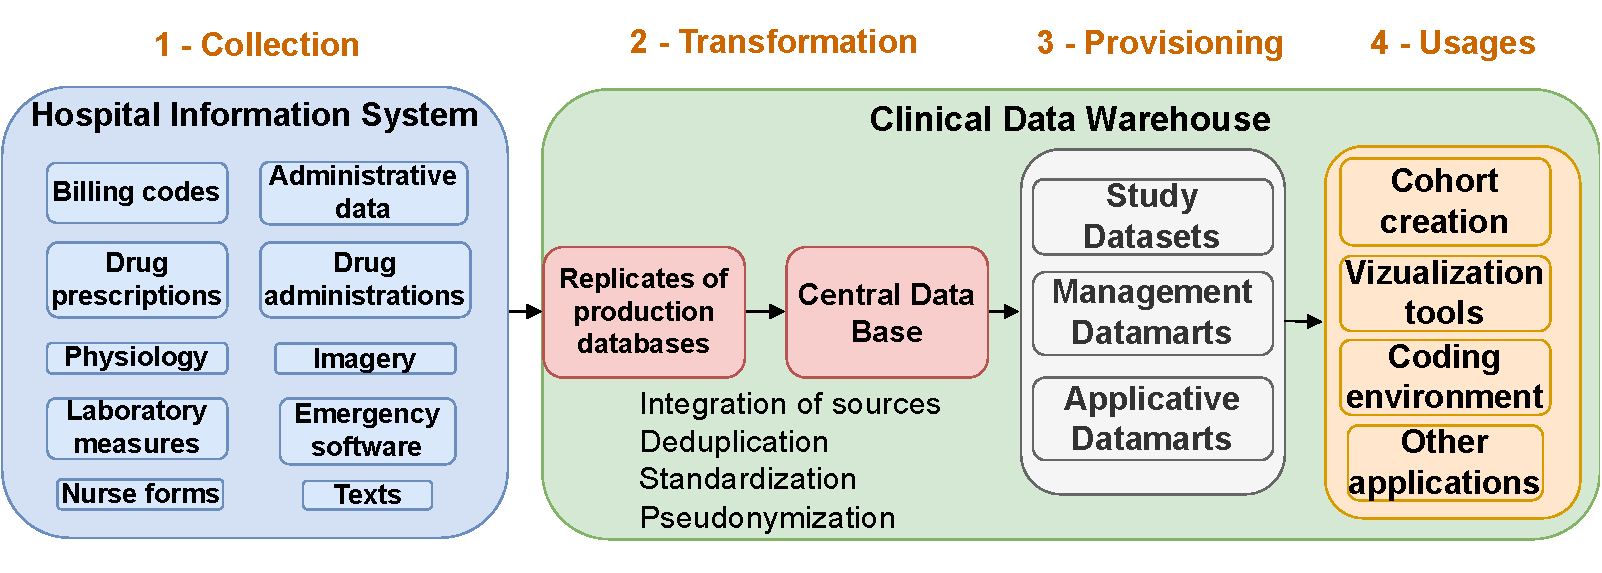
\includegraphics[width=1\linewidth]{img/chapter_2/Fig1.pdf}
  \caption{Clinical Data Warehouse: Four steps of data flow from the Hospital Information System: 1) collection, 2) transformations and 3) provisioning.}
  \label{background:CDW:fig:ehr_flow}
\end{figure*}


\section{Speaking to the data collectors: Interviews of French
  University Hospitals}\label{sec:cdw:methods}

Based on an overview of university hospital CDWs in France, this study make
general recommendations for properly leveraging the potential of CDWs to improve
healthcare. It focuses on: governance, transparency, types of
data, data reuse, technical tools, documentation and data quality control
processes.

Interviews were conducted from March to November 2022 with 32 French regional
and university hospitals, both with existing and prospective CDWs.

\subsection{Interviews and study coverage}\label{subsec:cdw:interviews}

\paragraph{Semi-structured interviews}

Semi-structured interviews were conducted on the following
themes: the initiation and construction of the CDWs; the current status of the
project and the studies carried out; opportunities and obstacles; quality
criteria for observational research. S1 Table list
all interviewed people with their team title. The complete form, with the
precised questions, is available in \ref{apd:cdw:interviews}.

The interview form was sent to participants in advance, and then used as a
support to conduct the interviews. The interviews lasted 90 minutes and were
recorded for reference.

\paragraph{Regional and university hospitals in France: different levels of maturity}

Scope of 32 CHUs, out of the 3000 care sites in France to yield exhaustive
conclusion on a restricted scope. Drive most specialized care, research in their
core mission. Date of interview

\paragraph{Focus on the 18 CDWs with highest level of maturity}

The denominator for the quantitative results is the 18 CDWs in production

\subsection{A classification of observational
  studies}\label{subsec:cdw:classification}

Contrast with classical epidemiology study types and the notion of experiment \citep{rothman2012epidemiology}.

\paragraph{Outcome frequency}
\paragraph{Population characterization}
\paragraph{Risk factors}
\paragraph{Treatment effect}
\paragraph{Development of diagnostic or prognostic algorithms}
\paragraph{Medical informatics}


\section{Observations from a rapidly evolving and heterogeneous
  ecosystem}\label{sec:cdw:results}

\subsection{Governance: CDW are federating multiple teams in the
  hospital}\label{subsec:cdw:results:governance}
\paragraph{Initiation and actors}
Figure temporality of CDW
Federating potential
Multiple departments involved
Multiple skills involved, strong ties with the academics
In-house solution development vs industrialization

\paragraph{Management of studies}

Scientific committee and project follow-up platform

\subsection{Uneven transparency of ongoing
  studies}\label{subsec:cdw:results:transparency} Uneven public reference on
hospital websites of ongoing studies.

\subsection{Triple usage of data: Research, management,
  clinic}\label{subsec:cdw:results:data}

\paragraph{Strong dependance to the HIS}

Data collected reflect data collection
Exemples, AP-HP, HCLs

\paragraph{Categories of Data}

Main functionalities of HIS are the same. Common base Details: Table Takeaway:
most of the current accessible data are billing, administrative and text,
importantly, low access to temporality.

\paragraph{Data reuse: Research}
Details of current study types.
Details of specialty of the principal investigator
Interest for research data network but lack of resources

\paragraph{Data reuse: CDW are used for monitoring and management}
Initialization for billing
Potential for professional feedbacks
Pharmacovigilance

\paragraph{Data reuse: Strong interest for CDW in the context of care}

Some CDWs develop specific applications that provide new functionalities
compared to care software. Search engines can be used to query all the
hospital's data gathered in the CDW, without data compartmentalization between
different softwares. Dedicated interfaces can then offer a unified view of the
history of a patient's data, with inter-specialty transversality, which is
particularly valuable in internal medicine. These cross-disciplinary search
tools also enable healthcare professionals to conduct rapid searches in all the
texts, for example, to find similar patients \citep{garcelon2017finding}.
%
There is a growing interest in such computational phenotyping tools to support
the development of digital health solutions \citep{wen2023impact}.
%
Uses for prevention, automation of repetitive tasks, and care coordination are
also highlighted. Concrete examples are the automatic sorting of hospital
prescriptions by order of complexity or the setting up of specialized channels
for primary or secondary prevention.

\subsection{A multi-layered technical
  architecture}\label{subsec:cdw:results:architecture} Three layer : Data
preprocessing (acquisition and normalization), storage, exposure Datalab: a
crucial technological brick

\subsection{Too little data quality and too many data
  formats}\label{subsec:cdw:results:data_quality}
\paragraph{Quality tools}
Automatic tooling for acquisition
First development for automatic data checks
\paragraph{Standard format}
No single standard data model,
Omop
eHop
\paragraph{Documentation}
Half of the CDWs have put in place documentation accessible within the organization
No documentation is public

\section{Recommendations: How to consolidate EHRs and expand
  usages}\label{sec:cdw:recommendations}

\subsection{Governance: CDWs are
  infrastructures}\label{subsec:cdw:recommendations:governance}

CDW becomes an essential component of data management in the hospital Resources
specific to the warehouse are rare and only project-based. Should promote
long-middle term teams (eg. inria ?) Multi-layered governance

\subsection{Transparency: Keep the bar
  high}\label{subsec:cdw:recommendations:transparency} Public registration of
comparative observational study protocols for research Patient information stays
limited

\subsection{Data: Complex data collection requires a variety of
  expertise}\label{subsec:cdw:recommendations:data} study design : change of
focus from data collection to data preprocessing -> other complementary skills
needed Link with the HIS, lack of standard at the HIS level, lack of sharing of
data schema Data reuse oriented towards primary care is still rare and rarely
supported by appropriate funding.


\subsection{Technical architecture: Towards more harmonization and open source ?
}\label{subsec:cdw:recommendations:architecture} Lack of harmonization: focus on
fewer solutions Commercial solutions emerging Case for open source:
transparency, less technological lock-in, mutualization, favor modularity, help
build consensus Opportunity for open source solutions Data quality, standard
formats Quality is not sufficiently considered as a relevant scientific topic
itself. Tooling: Link with devops/ automated CI in industrial data science there
is a need for open-source publication of research code to ensure quality
retrospective research

\subsection{Data quality an document: more incentives needed}\label{subsec:cdw:recommendations:quality}

Quality is not sufficiently considered as a relevant scientific topic itself.
However, it is the backbone of all research done within a CDW. In order to
improve the quality of the data with respect to research uses, it is necessary
to conduct continuous studies dedicated to this topic [52,54–56]. These studies
should contribute to a reflection on methodologies and standard tools for data
quality, such as those developed by the OHDSI research network [41].

Finally, there is a need for open-source publication of research code to ensure
quality retrospective research [55,57]. Recent research in data analysis has
shown that innumerable biases can lurk in training data sets [58,59]. Open
publication of data schemas is considered an indispensable prerequisite for all
data science and artificial intelligence uses [58]. Inspired by data set cards
  [58] and data set publication guides, it would be interesting to define a
standard CDW card documenting the main data flows.

\section{Conclusion}\label{sec:cdw:conclusion}

The French CDW ecosystem is beginning to take shape

The priority is the creation and perpetuation of multidisciplinary warehouse teams

Constitution of a multilevel collaboration network is another priority.

Common data model should be encouraged

The question of expanding the scope of the data beyond the purely hospital domain must be asked.

Heterogeneity of data collection calls for distributed information sharing models.

\chapter{Exploring a complexity gradient in representation and predictive algorithms for EHRs}\label{chapter:predictive_models}
\section{Abstract}\label{sec:predictive_models:abstract}

The previous chapter demonstrate the strong interest within French CDWs in using to develop
accurate prediction models.

\vfill
\textit{This chapter has not been submitted to any journals or conference until
  now.\\ XXX \\
  As the first author I formulated the research question, designed the study,
  performed the experiments and wrote the manuscript.}

\clearpage
\section{Predictive models in healthcare: Less fascination, more practical utility}\label{sec:predictive_models:motivation}

\subsection{Why such interest in predictive models in healthcare}\label{subsec:predictive_models:importance}

\paragraph{Interest in the clinic}

% better use of constrained medical resources
\textit{Being able to predict key outcomes could, theoretically, make the use of
  hospital palliative care resources more efficient and precise} \citep{topol2019high}

The Framingham risk score, one of the earliest predictive model in medicine was
designed to predict Coronary heart disease risk by fitting a cox model using
seven features on 5300 patients: age, cholesterol, systolic blood pressure,
hematocrit, ECG status, smoking at intake, and relative body weight
\citep{brand1976multivariate}.

\cite{harrell2001regression} mention diagnosis, prognosis, confounder adjustment
and heterogeneous treatment effects (mainly for cost-effectiveness analyses) as
the main uses of predictive models in healthcare. Ten years later,
\cite{steyerberg2009applications} also mentions diagnosis, prognosis and therapy
(He has a great figure from pubmed). I should do the same for 2023.

Some are used in clinical practice every day : the Glasgow coma scale
\citep{teasdale1974assessment}, the APACHE III score \citep{knaus1991apache}.
But a very small part of the published models are used in practice
\citep{wyatt1995commentary}. Reasons for this poor adoption are lack of
evidences for credibility, generalizability or clinical effectiveness.

Prevention : \textit{Early detection and appropriate treatment of sepsis have
  been associated with a significant mortality benefit in hospitalized patients}
\citep{wong2021external}

Alert systems \citep{yu2018artificial}.

Patient deterioration detection \citep{rothman2013development}: \textit{Rather than attempting to forecast a particular
  adverse event, we argue that intervention during early deterioration can help prevent such an adverse event from
  occurring}

\paragraph{Risk stratification}

risk stratify \citep{tang2007global}

\paragraph{Long term prevention}


\paragraph{Planning and piloting}

Rejoin the logistic and administrative help from \cite{topol2019high}.

The LOS task: planning the number of beds and members of staff required,
identifying individual outliers and case mix correction for benchmarking \citep{verburg2017models}

\paragraph{Exploring french CDWs:} 23 \% of studies, just after population definitions).

\subsection{Data sources fueling predictive models are increasingly complex}\label{subsec:predictive_models:complex_data}

Why is EHR so complex ? How ? time, high cardinality, multi-modality

\paragraph{In the literature}: early article in \cite{wu2010prediction},
literature review from 2017 \citep{goldstein2017opportunities}, literature
review more focused on models and task from soda prez.

Within french CDW(link with previous chapter)

\subsection{Low prevalence and local practice: Headaches for machine learning}\label{subsec:predictive_models:low_prevalence}

For logistic models, a requirement is that the test set should have at least 10
cases per feature with a positive event (eg. mortality)
\citep{harrell1985regression,wyatt1995commentary}.

\subsection{What makes a healthcare predictive model useful?}\label{subsec:predictive_models:useful}

What are the most impactful algorithms for predictive tasks from structured EHR
? A wealth of methods, but a lack of insights on the advantages and
inconvenience for specific problems and resources.

We build upon the criteria for adoption from \cite{wyatt1995commentary}.

More modern sources eg. \cite{subbaswamy2020development}.

\paragraph{We can share it easily: } Hence, people can use it AND contribute to
external validity and continuous improvements.

\paragraph{Performances} linked to accuracy, but questions on how to measure it.

\paragraph{Insertion in the care workflow}

Arguments for ease of deployment.

\section{From basic to complex: four increasingly sophisticated predictive pipelines}\label{sec:predictive_models:pipelines}

\subsection{Demographic features}\label{subsec:predictive_models:demographic}

\subsection{Count encoding with event features}\label{subsec:predictive_models:count_encoding}

\subsection{Static Embeddings of event features}

\subsection{Transformer based}\label{subsec:predictive_models:transformer}

\section{Empirical Study}\label{sec:predictive_models:empirical_study}

\subsection{Evaluation pipeline}\label{subsec:predictive_models:evaluation_pipeline}

\subsection{Three clinical and operational tasks}\label{subsec:predictive_models:task_definitions}

\paragraph{Length Of Stay: Plan}

\paragraph{Diagnosis Prediction: Benchmark}

\paragraph{Major Adverse Cardiovascular Events: Prevent}

\subsection{Results: Performance-sample trade-offs}

\section{Conclusion}\label{sec:predictive_models:conclusion}

\chapter{Prediction is not all we need: Causal analysis of EHRs to ground decision making}\label{chapter:causal_tuto}
\section{Abstract}\label{sec:causal_tuto:abstract}

\begin{citationbox}
  Nature marks each growth ... according to its curative benefit.
  \par\hfill -- Paracelsus
\end{citationbox}

\vfill
This chapter has been submitted to \textit{npj Digital Medicine} as:\\
\textit{Matthieu Doutreligne, Tristan Struja, Judith Abecassis, Claire Morgand, Gaël
  Varoquaux, \& Leo Anthony Celi. (2023). Step-by-step causal analysis of Electronic Health Records to ground
  decision making.} \\
As the first author I formulated the research question, designed the study,
performed the experiments and wrote the manuscript.

\clearpage
\section{Motivation : Healthcare is concerned with decision making, not mere
  prediction}%
\label{sec:causal_tuto:motivation}%


Even the early Framingham study concludes that risk reduction is more important
than identifying the strength of specific risk factors since this quantity is
subject to slight changes in the risk model \citep{brand1976multivariate}:
\textit{It further suggests that the strength of a particular risk factor may
  not be as important from the point of view of intervention as the ability to
  safely and conveniently achieve even a moderate risk reduction in a large number
  of persons.}
In a foundational article on EHR, the use-case of heart failure prediction is
motivated by agressive interventions \citep{wu2010prediction}: \textit{heart
  failure could potentially lead to improved outcomes through aggressive
  intervention, such as treatment with angiotensin converting enzyme
  (ACE)-inhibitors or Angiotensin II receptor blockers (ARBs).}. It is almost
always the case that prognosis models are motivated by decision making
processes. It is clearly described by \cite{steyerberg2009applications} for
diagnosis: \textit{If we do a diagnostic test, we may detect an underlying
  disease. But some diseases are not treatable, or the natural course might be
  very similar to what is achieved with treatment.}

\subsection{Predictive medicine currently suffers from biases}%
\label{subsec:causal_tuto:predictive_medicine_biases}%
(shortcuts,
population shifts). Racial, gender and under-served population biases raise
concern on fairness.

\subsection{A key ingredient to ground data-driven decision making is causal thinking}\label{subsec:causal_tuto:causal_thinking}

\subsection{The need for synthetic materials for practitioners}%
\label{subsec:causal_tuto:synthetic_materials}%

The relevant concepts for causal inference are scattered in different literatures. A dedicated exposition to time-varying data in EHRs would help practitioners and data scientists that study them.
\subsection{Motivating example}\label{subsec:causal_tuto:motivating_example}


\section{Step-by-step framework for robust decision making from EHR data}%
\label{sec:causal_tuto:framework}%

\subsection{Robust study design to avoid biases: Framing the question}%
\label{subsec:causal_tuto:framing}%

PICOT
Selection Bias
Immortal time bias

\subsection{Is the dataset sufficient to inform on the intervention: identification}%
\label{subsec:causal_tuto:identification}%
Causal graph Computing the causal effect of interest: Estimation Confounders
extractions Confounders aggregation Causal estimators Nuisance estimators

\begin{background_box_left}


  \paragraph{Causal Assumptions}\label{background:causal_assumptions}

  \md{Taken from "how to select": blend with literal explanations given in "causal tuto"}
  We assume the following four assumptions, referred as strong ignorability and
  necessary to assure identifiability of the causal estimands with observational
  data \citep{rubin_causal_2005}:
  \begin{assumption}[Unconfoundedness]\label{assumption:ignorability}
    \begin{equation*}\label{eq:ignorability}
      \{Y(0), Y(1) \} \indep A | X
    \end{equation*}
    This condition --also called ignorability-- is equivalent to the conditional
    independence on $e(X)$ \citep{rosenbaum_central_1983}: $\{Y(0), Y(1) \}
      \indep  A | e(X)$.
  \end{assumption}


  \begin{assumption}[Overlap, also known as Positivity)]\label{assumption:overlap}
    \begin{equation*}\label{eq:overlap}
      \eta < e(x) < 1 - \eta \quad \forall x \in \mathcal X \text{ and some } \eta > 0
    \end{equation*}
    The treatment is not perfectly predictable. Or with different words, every
    patient has a chance to be treated and not to be treated. For a given set of
    covariates, we need examples of both to recover the ATE.
  \end{assumption}

  As noted by \cite{damour_overlap_2020}, the choice of covariates $X$ can
  be viewed as a trade-off between these two central assumptions. A bigger
  covariates set generally reinforces the ignorability assumption. In the
  contrary, overlap can be weakened by large $\mathcal{X}$ because of the
  potential inclusion of instruments: variables only linked to the treatment which
  could lead to arbitrarily small propensity scores.

  % remark: There is a major counter example to these colliders (variables which
  % are caused by both the outcome and the treatment),

  \begin{assumption}[Consistency]\label{assumption:consistency} The observed
    outcome is the potential outcome of the assigned treatment:
    \begin{equation*}\label{eq:consistancy}
      Y = A \, Y(1) + (1-A) \, Y(0)
    \end{equation*}
    Here, we assume that the intervention $A$ has been well defined. This
    assumption focuses on the design of the experiment. It clearly states the link
    between the observed outcome and the potential outcomes through the
    intervention \citep{hernan_causal_2020}.
  \end{assumption}

  \begin{assumption}[Generalization]\label{assumption:generalization} The training
    data on which we build the estimator and the test data on which we make the
    estimation are drawn from the same distribution $\mathcal D^*$, also known as
    the ``no covariate shift'' assumption \citep{jesson_identifying_2020}.
  \end{assumption}

\end{background_box_left}

\subsection{Assessing the robustness of the hypothesis: Vibration or sensitivity
  analysis}%
\label{subsec:causal_tuto:vibration_analysis}%

Sensitivity vs robustness

\subsection{Heterogeneity of treatment}\label{subsec:causal_tuto:heterogeneity}

Interest of HTE
How to do HTE ? Final regression analysis.

\section{Application on MIMIC-IV}\label{sec:causal_tuto:application}

Emulated trial: Effect of albumin in combination with crystalloids compared to crystalloids alone on 28-day mortality in sepsis patients
Choice of the trial
Known effects

\subsection{Framing the question}\label{subsec:causal_tuto:framing_mimic}

\subsection{Identification}
Covariates and dag

\subsection{Estimation}\label{subsec:causal_tuto:estimation_mimic}
Confounders extractions
Confounders aggregation
Causal estimators
Nuisance estimators

\subsection{Vibration analysis}\label{subsection:causal_tuto:vibration_mimic}
Varying estimation choices:
Varying inclusion criteria: illustration of immortal time bias

\subsection{Heterogeneity of treatment}\label{subsec:causal_tuto:heterogeneity_mimic}

\section{Discussion}\label{subsec:causal_tuto:discussion}

%%%%%%%%%%%%%%%%%%%%%%% CHAPTER 5 %%%%%%%%%%%%%%%%%%%%%%%%%%%%%%%
\chapter{How to select predictive models for causal inference?}\label{chapter:causal_model_selection}

\begin{citationbox}
  Nature marks each growth ... according to its curative benefit.
  \par\hfill -- Paracelsus
\end{citationbox}

\begin{chapterabstract}
  % Predictive models are not sufficient for decision making: I showed it in
  % chapter 4
  In the previous chapters, we showed the strong interest in predictive models for
  healthcare, bridging to increasingly complex machine learning algorithms. We
  also pointed out that even when giving likely outcomes, they are not immediately
  transposable to decision making --choosing whether to treat or not to treat.
  Such reasoning on the effect of an intervention is a causal-inference task. We
  demonstrated that causal thinking was necessary to avoid introducing biases in
  the study design or during confounders selection.
  % Even with causal framework, there are too many models to choose from
  But, even with a robust causal framework, the practitioner is left to choose among
  the plethora of predictive models available for health data (some detailed in
  \ref{subsec:predictive_models:importance}). In a given situation, which of these
  models yield the most valid causal estimates?
  % scope of the paper 
  Here, we highlight that classic machine-learning model selection does not pick
  the best models for causal inference. Indeed, causal model selection should
  control both outcomes for each individual, treated or not treated, whereas only
  one outcome is observed.
  Theoretically, simple risks used in machine learning do not control causal
  effects when treated and non-treated population differ too much. More elaborate
  risks use ``nuisances'' re-weighting to approximate the causal error on the
  observed data. But does estimating these nuisances adds noise to model selection?
  % Contributions
  Drawing from an extensive empirical study, we outline an efficient causal
  model-selection procedure. To select the best predictive model to guide
  decisions: use the so-called $R\text{-risk}$, use flexible estimators to compute
  the nuisance models on the train set, and split out 10\% of the data to compute
  risks.
\end{chapterabstract}
%\section*{Abstract}\label{sec:causal_model_selection:abstract}

\vfill

\begin{footnotesize}
  This chapter has been submitted to \textit{Artificial Intelligence in Medicine} as:
  \\ \textit{Matthieu Doutreligne, Gaël Varoquaux. How to select predictive models for
    decision making or causal inference?. 2023. ⟨hal-03946902v3⟩. \\
    As the first author I formulated the research question, designed the study, did the proves
    of the theoretical part, performed the experiments and wrote the manuscript.}
\end{footnotesize}

\clearpage
\section{Motivation: causal predictive models cannot rely on the Machine Learning
  toolbox}\label{sec:causal_model_selection:motivation}

\subsection{Extending prediction to prescription needs causality}\label{subsec:causal_model_selection:extending_prediction}

\md{watchout that I did not say the same thing as in chapter 4}
\paragraph{Progress in machine learning brings predictive models to new health
  data} \citep{beam2018big,rajkomar2019machine}, with the promise of precision
medicine. Automated analysis of medical images is increasingly accurate,
\emph{eg} for brain images, \citep{khojaste2022deep,zhang2019radiological} or
mammography \citep{yala2019deep,shen2019deep,nassif2022breast}. New prognostic
models leverage routinely-collected patient records \citep{mooney2018bigdata}:
predicting heart failure from claims \citep{desai2020comparison}, suicide
attempts from questionnaires \citep{simon2018predicting}... Clinical notes
contain much prognostic information but require text modeling
\citep{horng2017creating,wang2020prediction,spasic2020clinical,
  jiang2023health}. Data may be difficult to control and model, but the accuracy
of the prediction can be verified on left-out data
\citep{altman2009prognosis,poldrack2020establishment,varoquaux2022evaluating}.
Given a model predicting a health outcome, precision medicine would like it to
guide decisions: will an individual benefit from an intervention such as
surgery \citep{fontana2019can}? Contrasting predictions with and without the
treatment gives an answer, but statistical validity requires causal inference
\citep{snowden_implementation_2011,blakely2020reflection}.

% - Causal inference is difficult
% - Beyond the dream of assessing effectiveness and safety in real-word
%   practice \citep{black1996we} include off-label drug usage 
%   \citep{radley2006off} (which may lead to drug repurposing)
% - Plug in that outcome modeling is complementary to RCTs: observational
%   data gives weaker evidence than trials, but on both data outcome
%   modeling opens the door to individual.
% - Epidemiology has focused on propensity-score methods
% - Principle causal inference with outcome models is possible
% - It brings the promises of \emph{individualized treatment effects} --a
%   goal related to capturing heterogeneity and thus CATE--
% - It also performs well on causal-inference competition, although they
%   focused on the ATE

% The plethora of approaches approaches give different causal-inference
% estimates => need for guideline on causal model selection.

\paragraph{Causal-inference bridges to predictive modeling via the rich statistical literature on \emph{outcome
    models},} or G-computation, G-formula \citep{robins_role_1986}, Q-model \citep{snowden_implementation_2011}, conditional
mean regression \citep{wendling_comparing_2018}. A central challenge of inference of treatment effects is that of
confounding: spurious associations between treatment allocation and baseline health, \emph{eg} only prescribing a drug
to mild cases \citep{hernan_causal_2020,vanderweele2019principles}. Controlled allocation of treatment, as in randomized
controlled trials (RCTs), alleviate this concern. Yet most machine-learning models are trained on \emph{observational}
data, close to real-word practice \citep{black1996we,hernan_methods_2021} but challenging for causal inference. Causal
inference has been central to epidemiology, typically with methods that model treatment assignment
\citep{austin_moving_2015,grose_use_2020}, based on propensity scores \citep{rosenbaum_central_1983}. Recent empirical
results \citep{wendling_comparing_2018,dorie_automated_2019} show benefits of outcome modeling to estimate average
treatment effects. Maybe a greater benefit is that these methods naturally go beyond average effects, estimating
individualized or conditional average treatment effects (CATE), central to precision medicine.
%
For this purpose, such methods are also invaluable on randomized trials
\citep{su2018random,lamont2018identification,hoogland2021tutorial}.

\paragraph{Explosion of outcome modeling or machine learning methods.}
Many deep-learning methods have been developed for medical
image analysis \citep{shen2017deep,monshi2020deep}.
Even outcome-modeling methods specifically designed for causal
inference are numerous: Bayesian Additive Regression Trees
\citep{hill_bayesian_2011}, Targeted Maximum Likelihood Estimation
\citep{laan_targeted_2011,schuler_targeted_2017}, causal boosting
\citep{powers_methods_2018}, causal multivariate adaptive regression
splines \citep{powers_methods_2018}, random forests
\citep{wager_estimation_2018, athey_generalized_2019},
Meta-learners \citep{kunzel_metalearners_2019}, R-learners
\citep{nie_quasioracle_2017}, Doubly robust estimation
\citep{chernozhukov_double_2018}...
%\idea{The variety of estimators calls for model selection procedures}
The wide variety of methods raises the problem
of selecting between different estimators based on the data at hand.
%
Indeed, estimates of treatment effects can vary markedly across different
predictive models. For instance, Figure \ref{fig:acic_2016_ate_heterogeneity} shows
large variations obtained across different outcome estimators on
semi-synthetic datasets \citep{dorie_automated_2019}. Flexible models
such as random forests are doing well in most settings except
when treated and untreated populations differ noticeably, in
which case a linear model (ridge) is to be preferred.
However random forests with different hyper-parameters
(max depth= 2) yield poor estimates.
A simple rule of thumb such as preferring flexible models does not work in
general; model selection is needed.

\begin{figure}[h!]
  \begin{minipage}{.3\linewidth}
    \caption{\textbf{Different outcome models lead to different
        estimation errors on the Average Treatment Effects},
      on 77 classic simulations with known true causal effect
      \citep{dorie_automated_2019}. The different models are ridge regression
      and random forests with different hyper-parameters
      (details
      \ref{apd:toy_example:acic_2016_ate_variability}). The different configurations are
      plotted as a function of increasing difference between treated and
      untreated population --see
      \autoref{subsec:causal_model_selection:measuring_overlap}.
      There is no systematic best performer; data-driven model
      selection is important.
      \label{fig:acic_2016_ate_heterogeneity}
    }
  \end{minipage}
  \hfill
  \begin{minipage}{.65\linewidth}
    %\centering
    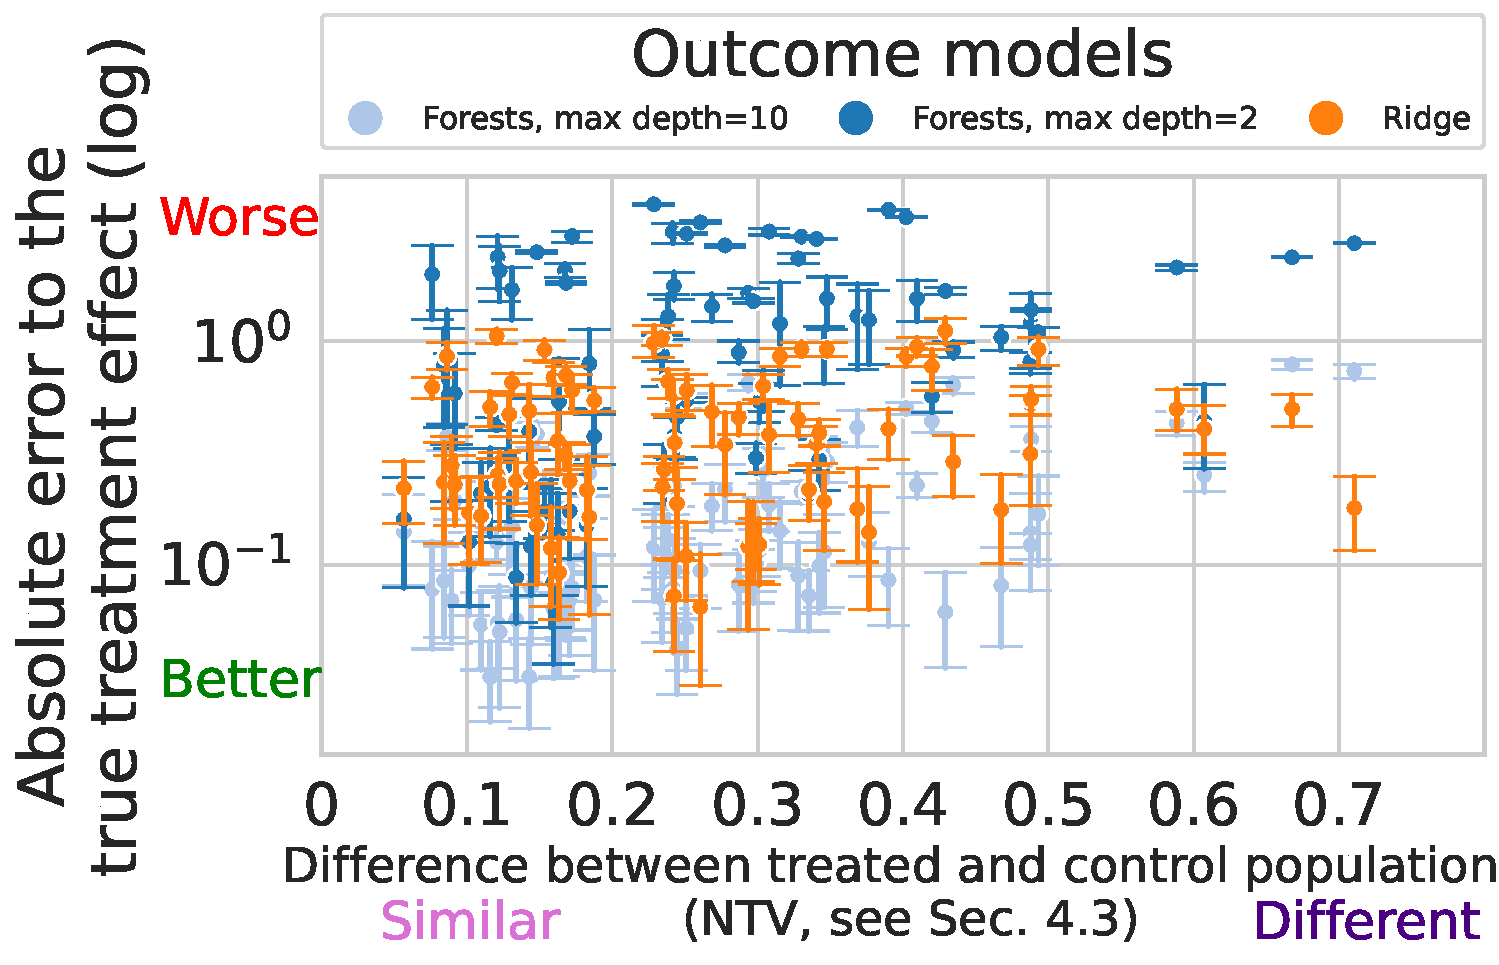
\includegraphics[width=\linewidth]{img/chapter_5/_2023-03-08-11-10-28_acic_2016_ate_heterogeneity.parquet_abs_bias_ylog_scale=True.pdf}%
  \end{minipage}
\end{figure}

Standard practices to select models in predictive settings rely on
the error on the outcome
\citep{poldrack2020establishment,varoquaux2022evaluating}. However, as we
will see, these practices may not pick the best models
for causal inference, as they can be misled by inhomogeneities due to
treatment allocation.
%
Given complex, potentially noisy, data, which model is to be most trusted to
yield valid causal estimates? As no single learner performs
best on all data sets, there is a pressing need for clear guidelines to select
outcome models for causal inference.

\paragraph{Objectives and structure of the chapter}

In this chapter, we study \textit{model selection procedures}
in practical settings: \textit{finite samples} settings and without
\textit{well-specification} assumption. Asymptotic causal-inference
theory calls for complex risks, but a practical question is
whether model-selection procedures, that rely on data split, can estimate
these risks reliably enough. Indeed, they
come with more quantities to estimate, which may
bring additional variance, leading to worse model selection.

We first illustrate the problem of causal model
selection and briefly review prior art. Then, Section
\ref{sec:causal_model_selection:setting} sets causal model selection in the
\emph{potential outcome} framework and details the causal risks and
model-selection procedure. Section \ref{sec:theory} gives theoretical
results. Section \ref{sec:empirical_study} details a thorough empirical
study, covering many different settings. Finally, Section \ref{sec:discussion}
discusses the findings.
%
Results outline how to best select outcome models for causal
inference with an adapted
cross-validation to estimate the so-called $R\mathrm{-risk}$.
This risk compensates for systematic
differences between treated and non-treated individuals using
two \emph{nuisance} models,
themselves estimated from data and thus imperfect; yet these
imperfections do not undermine the $R\mathrm{-risk}$.


\subsection{Illustration: the best predictor may not estimate best causal
  effects}%
\label{subsec:causal_model_selection:illustration}%


\begin{figure}[t!]
  \begin{minipage}{0.32\textwidth}
    \caption[The best predictor may not estimate best causal
      effects]{\textbf{Illustration} \\a) a random-forest estimator
      with high performance for standard prediction (high $R^2$) but that
      yields poor causal estimates (large error between true effect $\tau$ and
      estimated $\hat{\tau}$), b) a linear estimator with smaller
      prediction performance leading to better causal estimation. \\[1ex]
      Selecting the estimator with the smallest error to the individual
      treatment effect $\mathbb{E}[(\tau(x) - \hat{\tau}(x))^2]$
      --the $\tau\text{-risk}$, def.\,\ref{def:tau_risk} -- would lead to
      the best causal estimates; however computing this error is not
      feasible: it requires access to unknown quantities:
      $\tau(x)$. \\[1ex]
      While the random forest fits the data better than the linear model, it
      gives worse causal inference because its error is inhomogeneous between
      treated and untreated. The $R^2$ score does not capture this
      inhomogeneity.
      \label{fig:toy_example}
    }
  \end{minipage}
  \hfill
  \begin{minipage}{0.65\textwidth}
    %\centering
    {\sffamily\footnotesize\scalebox{0.9}{a) Random forest, good average prediction but bad
        causal inference}}

    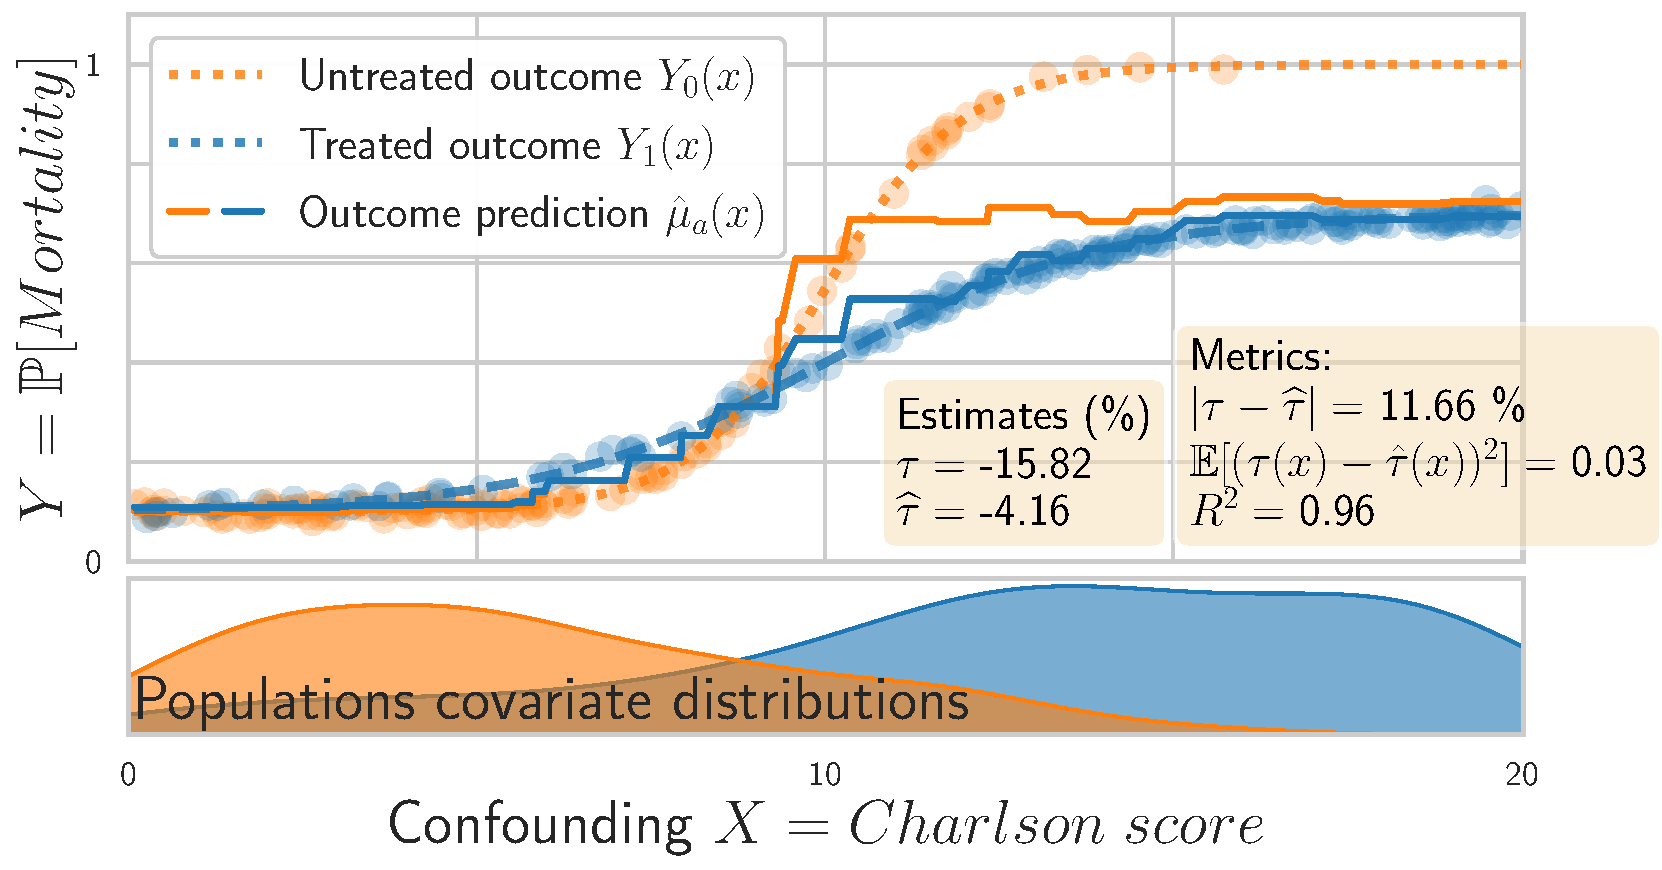
\includegraphics[width=1\linewidth]{img/chapter_5/toy_random_forest_high_R2_high_tau_risk.pdf}%

    {\sffamily\footnotesize\scalebox{0.9}{b) Linear model, worse average
        prediction but better causal inference}}

    \hfill%
    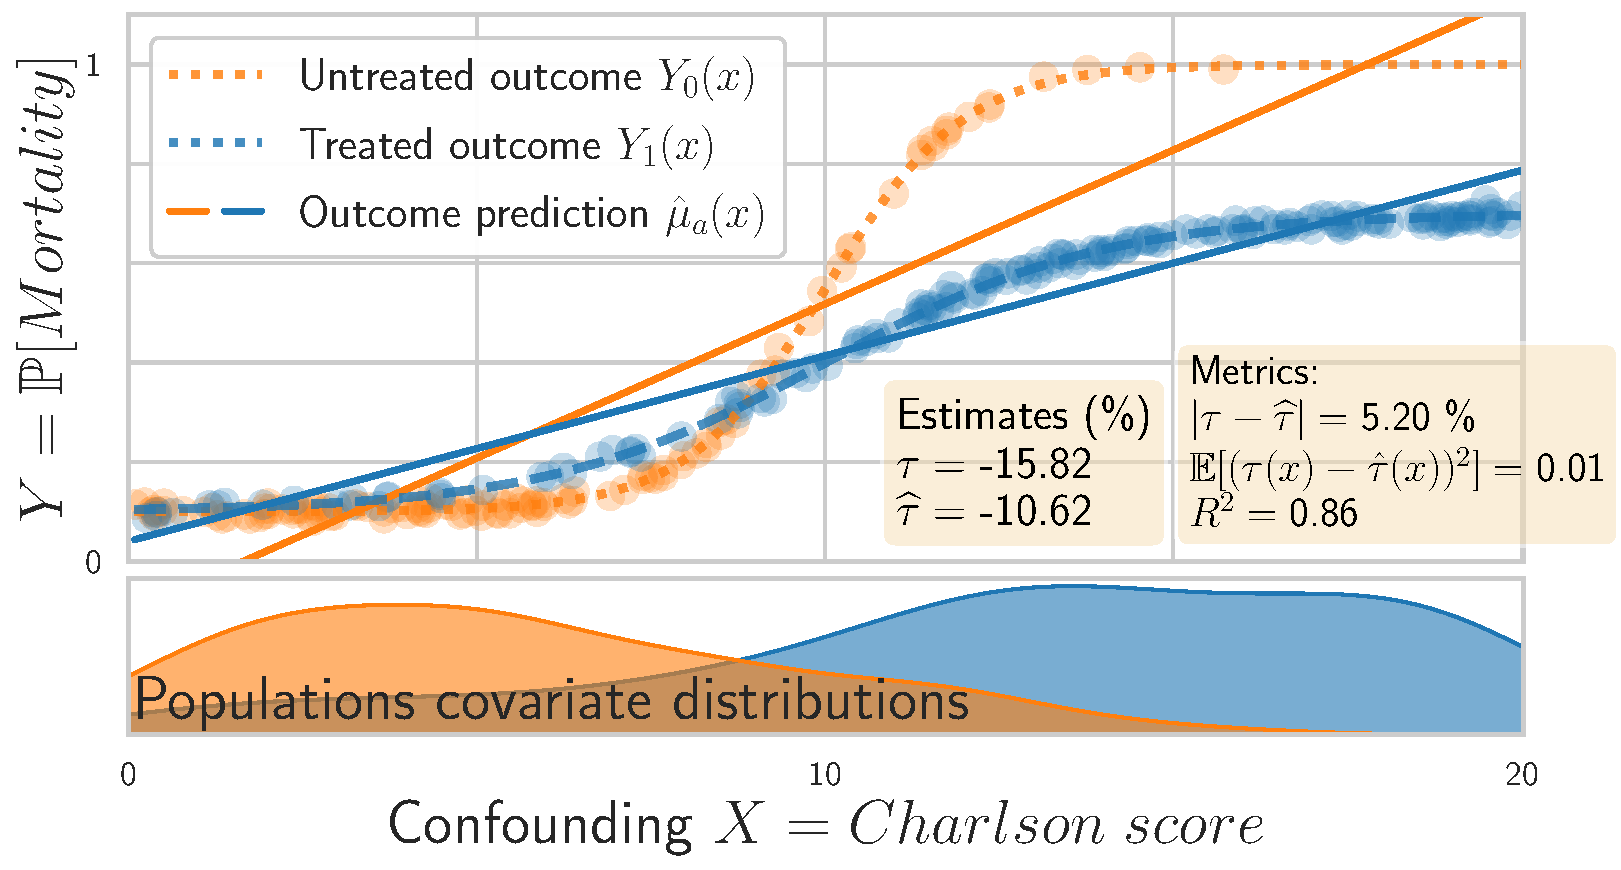
\includegraphics[width=1\linewidth]{img/chapter_5/toy_tlinear_model_small_R2_small_tau_risk.pdf}%
  \end{minipage}
\end{figure}


Using a predictor to reason on causal effects relies on contrasting the
prediction of the outcome for a given individual with and without the
treatment --as detailed in \autoref{sec:causal_model_selection:setting}.
%
Given various predictors of the outcome, which one should we use?
%
Standard predictive modeling or machine-learning practice selects the
predictor that minimizes the expected error.
However, this predictor may not be the best model to reason about
causal effects of an intervention, as we illustrate below.

Figure \ref{fig:toy_example} gives a toy example: the probability $Y$ of
an undesirable
outcome (\emph{eg} death), a binary treatment $A \in \{0, 1\}$, and a covariate
$X \in \mathbb R$ summarizing the patient health status (eg. the
Charlson index \citep{charlson_new_1987}). We simulate a
treatment beneficial (decreases $Y$) for patients with high Charlson scores (bad health
status) but with little effect for patients in good
condition (low Charlson scores).


Figure \ref{fig:toy_example}a shows a random forest predictor with a
counter-intuitive behavior: it predicts well on average the outcome (as measured
by a regression $R^2$ score) but perform poorly to estimate causal quantities:
the average treatment effect $\tau$ (as visible via the error $|\tau -
  \hat{\tau}|$) or the conditional average treatment effect (the error
$\mathbb{E}[(\tau(x) - \hat{\tau}(x))^2]$, called CATE).
%
On the contrary, Figure \ref{fig:toy_example}b shows a linear model with
smaller $R^2$ score but better causal inference.%

The problem is that causal estimation requires controlling
an error on both treated and non-treated outcome for the same individual:
the observed outcome, and the non-observed \emph{counterfactual} one.
The linear model is misspecified --the outcome functions are not
linear--, leading to poor $R^2$; but it interpolates better to regions
where there are few untreated individuals --high Charlson score-- and
thus gives better causal estimates. Conversely, the random forest puts
weaker assumptions on the data, thus has higher $R^2$ score but is biased
by the treated population in the poor-overlap region, leading
to bad causal estimates.

This toy example illustrates that the classic minimum Mean Square Error
criterion is not suited to choosing a model among candidate
estimators for causal inference.

\subsection{Prior work: model selection for outcome modeling (g-computation)}\label{subsec:causal_model_selection:prior_work}%


A natural way to select a predictive model for causal inference would be
an error measure between a causal quantity such as the CATE and models' estimate. But such error is
not a ``feasible'' risk: it cannot be computed solely from observed data
and requires oracle knowledge.

% XXX: I think that I should make the following paragraph shorter

\paragraph{Simulation studies of causal model selection}

Using eight simulations setups from \cite{powers_methods_2018}, where
the oracle CATE is known, \citet{schuler_comparison_2018} compare four
causal risks, concluding that for CATE estimation the best
model-selection risk is the so-called $R\text{-risk}$
\citep{nie_quasioracle_2017} --def.\,\ref{def:r_risk}, below. Their
empirical results are clear for randomized treatment allocation but less
convincing for observational settings where both simple Mean Squared
Error --MSE, $\mu\text{-risk}(f)$ def.\,\ref{def:mu_risk}-- and
reweighted MSE --$\mu\text{-risk}_{IPW}$ def.\,\ref{def:mu_ipw_risk}--
appear to perform better than $R\text{-risk}$ on half of the simulations.
Another work \citep{alaa_validating_2019} studied empirically both MSE and
reweighted MSE risks on the semi-synthetic ACIC 2016 datasets
\citep{dorie_automated_2019}, but did not include the $R\text{-risk}$. We complete these
prior empirical work by studying a wider variety of data generative
processes and varying the influence of overlap, an important parameter of
the data generation process which makes a given causal metric appropriate
\citep{damour_overlap_2020}. We also study how to best adapt
cross-validation procedures to causal metrics which themselves come with
models to estimate.

\paragraph{Theoretical studies of causal model selection}

Several theoretical works have proposed causal model selection procedures
that are \emph{consistent}: select the best model in a family given
asymptotically large data. These work rely on introducing a
CATE estimator in the testing procedure: matching
\citep{rolling_model_2014}, an IPW estimate
\citep{gutierrez_causal_2016}, a doubly robust estimator
\citep{saito_counterfactual_2020}, or debiasing the error with influence
functions \citep{alaa_validating_2019}. However, for theoretical
guarantees to hold, the test-set correction needs to converge to the
oracle: it needs to be flexible enough --well-posed-- and asymptotic
data. From a practical perspective, meeting such requirements
implies having a good CATE estimate, thus having solved
the original problem of causal model selection.

\paragraph{Statistical guarantees on causal estimation procedures}

Much work in causal inference has focused on procedures that
guarantee asymptotically consistent estimators, such as Targeted
Machine Learning
Estimation (TMLE) \citep{laan_targeted_2011,schuler_targeted_2017} or
Double Machine Learning \citep{chernozhukov_double_2018}. Here also, theories require asymptotic regimes and
models to be \textit{well-specified}.

By contrast, \citet{johansson2022generalization} studies causal estimation
without assuming that estimators are well specified. They derive an upper bound
on the oracle error to the CATE ($\tau\text{-risk}$) that involves the error on
the outcome and the similarity of the distributions of treated and control
patients. However, they use this upper bound for model optimization,
and do not give insights on model selection. In addition, for hyperparameter
selection, they rely on a plugin estimate of the $\tau\text{-risk}$ built with
counterfactual nearest neighbors, which has been shown ineffective
\citep{schuler_comparison_2018}.


\begin{background_box_left}

  \section{Formal setting: causal inference and model selection}%
  \label{sec:causal_model_selection:setting}%

  \subsection{The Neyman-Rubin Potential Outcomes framework}%
  \label{subsec:causal_model_selection:framework}%

  \paragraph{Settings} We consider the Potential Outcomes framework introduced in
  \ref{par:intro:causal_framework:neyman_rubin}.

  \paragraph{Causal assumptions}\label{par:causal_assumptions}

  Assumptions are necessary for causal estimands to be
  identifiability
  in observational settings \citep{rubin_causal_2005}. We assume the usual
  strong ignorability assumptions: \emph{1)}
  \emph{unconfoundedness} \mbox{$\{Y(0),
      Y(1) \} \indep A | X$}, \emph{~2)} \emph{strong overlap} ie. every patient has a
  strictly positive probability to receive each treatment, \emph{3)}
  \emph{consistency}, and \emph{4)} \emph{generalization} (introduced in
  \ref{subsec:causal_tuto:identification}).

  \paragraph{Estimating treatment effects with outcome models}\label{subsec:estimators}

  Should we know the two expected outcomes for a given $X$,
  we could compute the
  difference between them, which gives the causal effect of the treatment.
  %
  These two expected outcomes can be computed from the observed data:
  the consistency \ref{assumption:consistency} and unconfoundedness
  \ref{assumption:ignorability} assumptions imply the equality of two different
  expectations:
  \begin{equation}\label{eq:mu_identification}
    \mathbb E_{Y(a) \sim \mathcal{D^{\star}}} [Y(a)|X=x] = \mathbb E_{Y \sim \mathcal{D}} [Y|X=x, A=a]
  \end{equation}
  On the left, the expectation is taken on the counterfactual unobserved
  distribution. On the right, the expectation is taken on the factual observed
  distribution conditionally on the treatment. This equality is referred as the
  g-formula identification \citep{robins_new_1986}. For the rest of the
  paper, the expectations will always be taken on the factual observed
  distribution $\mathcal{D}$. This identification leads to outcome based estimators (ie.
  g-computation estimators \citep{snowden_implementation_2011}), targeting the
  ATE $\tau$ with outcome modeling:
  \begin{eqnarray}
    \tau =& \mathbb E_{Y \sim \mathcal{D^{\star}}}[Y(1) - Y(0)|X=x]
    = \mathbb E_{Y \sim \mathcal{D}}[Y|A=1] - \mathbb E_{Y \sim \mathcal{D}}[Y| A=0]
    \label{eq:tau_population}
  \end{eqnarray}
  This equation builds on two quantities: the conditional expectancy
  of the outcome given the covariates and either
  treatment or no no treatment, called \emph{response function}:
  \begin{flalign*}
    \text{Response function}
     &  &
    \mu_{a}(x) \myeq \; \mathbb E_{Y \sim \mathcal{D}} [Y|X=x, A=a]
     &  &
  \end{flalign*}

  Given a sample of data and the oracle response functions $\mu_0, \mu_1$, the
  finite sum version of \autoref{eq:tau_population} leads to an
  estimator of the ATE written:
  \begin{equation}
    \hat \tau = \frac{1}{n} \biggl(\sum_{i=1}^n \mu_{1}(x_i) - \mu_{0}(x_i) \biggr)
    \label{eq:ate_estimate}
  \end{equation}
  This estimator is an oracle \textbf{finite sum estimator} by opposition to the
  population expression of $\tau$, $\mathbb{E}[\mu_{1}(x_i) - \mu_{0}(x_i)]
  $,
  which involves an expectation taken on the full
  distribution $\mathcal D$, which is observable but requires infinite data. For
  each estimator $\ell$ taking an expectation over $\mathcal D$, we use the symbol
  $\hat \ell$ to note its finite sum version.

  Similarly to the ATE, at the individual level, the CATE:
  \begin{equation}
    \tau(x) = \mu_{1}(x) - \mu_{0}(x)
    \label{eq:cate_estimate}
  \end{equation}

  \paragraph{Robinson decomposition}
  The \emph{R-decomposition}
  of the outcome model plays an important role,
  \citep{robinson_rootnconsistent_1988}:
  introducing two quantities, the conditional mean outcome
  and the probability to be treated (known as propensity score \citep{rosenbaum_central_1983}):
  \begin{flalign}
    \text{Conditional mean outcome} &                    & m(x) \myeq \; & \mathbb E_{Y \sim
    \mathcal{D}} [Y|X=x]            &                    &
    \label{def:m}
    \\
    \text{Propensity score}         &                    &
    e(x) \myeq \;                   & \mathbb P[A=1|X=x]
    \label{def:propensity_score}
  \end{flalign}
  the outcome can be written
  \begin{flalign}\label{eq:r_decomposition}
    \text{R-decomposition}                                                                   &  & y(a) = m(x) + \big( a - e(x) \big)
    \tau(x) + \varepsilon(x; a) \quad \text{with}\quad \mathbb E[\varepsilon(X; A)|X, A] = 0 &  &
  \end{flalign}
  $m$ and $e$ are often called
  \emph{nuisances} \citep{chernozhukov_double_2018}; they are unknown.

\end{background_box_left}

%As noted by \citep{johansson2022generalization}, the machine learning
%community often referred to the CATE by ITE, the Individual Treatment Effect.
%From a purely causal point of view, the ITE is uniquely defined for each
%individual and might not be accessible: $ITE(x_i) = Y_i(1) -  Y_i(0)$. On the
%contrary, the CATE can always be derived by taking conditional expectancies. It
%is the expected effect of the treatment in the region of the covariate space
%around X. %Too cultivate

\begin{table*}[!tb]
  %\makebox[\textwidth]{
  \caption{Review of causal risks
    ---
    The $R\text{-risk}^*$ is called $\tau \text{-risk}_R$ in
    \citet{schuler_comparison_2018}.
    \label{tab:evaluation_metrics}}
  \resizebox*{\textwidth}{!}{
    \begin{threeparttable}[b]
      \centering
      \begin{tabular}{llr}
        \toprule
        Risk                                                                                           & Equation
                                                                                                       & Reference                                                                                                                                           \\
        \midrule
        $mse(\tau(X), \tau_f(X))=\tau\text{-risk}$                                                     & $\mathbb E_{X\sim
              p(X)}[(\tau(X) - \hat \tau_f(X))^2] $
                                                                                                       & Eq. \ref{eq:tau_risk} \citep{hill_bayesian_2011}                                                                                                    \\
        $mse(Y, f(X)) = \mu\text{-risk}$                                                               & $\mathbb{E}_{(Y, X, A)
            \sim \mathcal D}\left[(Y-f(X ; A))^2 \right]$
                                                                                                       & Def. \ref{def:mu_risk} \citep{schuler_comparison_2018}                                                                                              \\
        $\mu\text{-risk}_{IPW}^*$                                                                      & $\mathbb{E}_{(Y, X, A)
            \sim \mathcal D}\left[ \Big( \frac{A}{e(X)} + \frac{1-A}{1-e(X)} \Big)
        (Y-f(X ; A))^2 \right]$                                                                        & Def.
        \ref{def:mu_ipw_risk} \citep{vanderlaan_unified_2003}                                                                                                                                                                                                \\
        $\tau\text{-risk}^{\star}_{IPW}$                                                               & $\mathbb{E}_{(Y, X, A) \sim \mathcal D} \left[ \Big(Y \left( \frac{A}{e(X)} - \frac{1-A}{1-e(X)}\right)-\hat \tau_f\left(X\right)\Big)^2 \right]$ &
        Def. \ref{def:tau_ipw_risk} \citep{wager_estimation_2018}
        \\
        $U\text{-risk}^*$                                                                              & $\mathbb{E}_{(Y, X, A) \sim \mathcal D}  \big[
        \big( \frac{Y-m\left(X\right)}{A-e\left(X\right)} -  \hat \tau_f\left(X\right)\big)^{2} \big]$ &
        Def. \ref{def:u_risk} \citep{nie_quasioracle_2017}
        \\
        $R\text{-risk}^*$                                                                              & $\mathbb{E}_{(Y, X, A)
            \sim \mathcal D} \big[\big(\left(Y-m\left(X\right)\right)
        -\left(A-e\left(X\right)\right) \hat \tau_f\left(X\right)\big)^{2} \big]$                      &
        Def. \ref{def:r_risk} \citep{nie_quasioracle_2017}
        \\
        \bottomrule
      \end{tabular}
    \end{threeparttable}
  }
\end{table*}


\subsection{Model-selection risks, oracle and feasible}\label{subsec:causal_model_selection:causal_model_selection}

\paragraph{Causal model selection}

We formalize model selection for causal estimation. Thanks to the g-formula
identification (\autoref{eq:mu_identification}), a given outcome model $f: \mathcal X
  \times \mathcal A \rightarrow \mathcal{Y}$ --learned from data or built from
domain knowledge-- induces feasible estimates of the ATE and CATE (eqs
\ref{eq:ate_estimate} and \ref{eq:cate_estimate}), $\hat \tau_{f}$ and $\hat \tau_{f}(x)$.
%
Let $\mathcal F=\{f: \mathcal X \times \mathcal A \rightarrow \mathcal{Y}\}$ be
a family of such estimators. Our goal is to select the best candidate in this
family for the observed dataset $O$ using a risk
$\ell$:
\begin{equation}
  f^*_{\ell} = \argmin_{f \in \mathcal{F}} \ell(f, O)
  \label{eq:causal_model_selection}
\end{equation}

We now detail possible risks $\ell$, risks useful for causal
model selection, and how to compute them.


\paragraph{The $\tau\text{-risk}$: an oracle error risk}\label{paragraph:oracle_metrics}
%
As we would like to target the CATE, the following
evaluation risk is natural:
\begin{definition}[$\tau\text{-risk}(f)$]\label{def:tau_risk} also called PEHE
  \citep{schulam_reliable_2017, hill_bayesian_2011}:
  \begin{equation*}\label{eq:tau_risk}
    \tau\text{-risk}(f) = \mathbb E_{X\sim p(X)}[(\tau(X) - \hat \tau_f(X))^2]
  \end{equation*}
\end{definition}

Given observed data from $p(X)$, the expectation is computed with a
finite sum, as in eq.\,\ref{eq:ate_estimate}, to give an estimated
value $\widehat{\tau\text{-risk}}(f)$.
%
However this risk is not feasible as the oracles $\tau(x)$ are
not accessible with the observed data $(Y, X, A) \sim \mathcal D$.

\paragraph{Feasible error risks}\label{paragraph:feasible_metrics}
\emph{Feasible} risks are based on the prediction error of the outcome model
and \emph{observable} quantities.

All expectations below are on observed distribution:
$(Y, X, A) \sim \mathcal D$.

\begin{definition}[Factual $\mu\text{-risk}$]\label{def:mu_risk}
  \citep{shalit_estimating_2017} This is the usual Mean Squared Error on
  the target y. It is what is typically meant by ``generalization error'' in
  supervised learning:
  \begin{equation*}\label{eq:mu_risk}
    \mu\text{-risk}(f)=\mathbb{E}\left[(Y-f(X ; A))^2 \right]
  \end{equation*}
\end{definition}

We now detail risks that use the nuisances $e$
--propensity score, def \ref{def:propensity_score}-- and $m$ --conditional mean
outcome, def \ref{def:m}. We give the definitions as \textit{semi-oracles},
function of the true unknown nuisances, but later instantiate them with estimated
nuisances, noted $\big(\check e, \check m \big)$. Semi-oracles risks are
superscripted with the $^{\star}$ symbol.


\begin{definition}[$\mu\text{-risk}_{IPW}^{\star}$]\label{def:mu_ipw_risk}
  \citep{vanderlaan_unified_2003} Let the inverse propensity weighting
  function $w(x, a) = \frac{a}{e(x)} + \frac{1 - a}{1 - e(x)}$, we define the
  semi-oracle Inverse Propensity Weighting risk,
  \begin{equation*}\label{eq:mu_ipw_risk}
    \mu\text{-risk}_{IPW}^{\star}(f) = \mathbb{E}\left[ \Big( \frac{A}{e(X)} + \frac{1-A}{1-e(X)} \Big) (Y-f(X ; A))^2 \right]
  \end{equation*}
\end{definition}

\smallskip


\begin{definition}[$\tau\text{-risk}^{\star}_{IPW}$]\label{def:tau_ipw_risk}
  \citep{wager_estimation_2018}
  The CATE $\tau(x)$ can be estimated with a
  regression against inverse propensity weighted outcomes \citep{
    athey2016recursive,gutierrez_causal_2016,wager_estimation_2018},
  the $\tau\text{-risk}_{IPW}$.
  \begin{equation*}
    \tau\text{-risk}^{\star}_{IPW}(f) =\mathbb{E}
    \left[ \Big(Y \frac{A - e(X)}{e(X)
        (1-e(X))}-\tau_f\left(X\right)\Big)^2 \right]
    %  =\mathbb{E}_{(Y, X, A)
    %            \sim \mathcal D} \left[ \left(Y \left( \frac{A}{e(X)} -
    %            \frac{1-A}{1-e(X)}\right)-\tau_f\left(X\right)\right)^2 \right]
  \end{equation*}
\end{definition}

\begin{definition}[$U\text{-risk}^{\star}$]\label{def:u_risk}
  \citep{kunzel_metalearners_2019,nie_quasioracle_2017} Based on
  the Robinson decomposition --eq. \ref{eq:r_decomposition}, the U-learner
  uses the $A-e(X)$ term
  in the denominator. The derived risk is:
  \begin{equation*}
    U\text{-risk}^{\star}(f) =\mathbb{E}
    \left[
      \left( \frac{Y-m\left(X\right)}{A-e\left(X\right)} -
      \tau_f\left(X\right)\right)^{2} \right]
  \end{equation*}
  Note that extreme propensity weights in the
  denominator term might inflate errors in the numerator due to imperfect
  estimation of the mean outcome $m$.
\end{definition}

\begin{definition}[$R\text{-risk}^{\star}$]\label{def:r_risk}
  \citep{nie_quasioracle_2017,schuler_comparison_2018}
  The $R\text{-risk}$ also uses two nuisance $m$ and $e$:
  \begin{equation*}
    R\text{-risk}^{\star}(f) =\mathbb{E} \big[
      \big(\left(Y-m\left(X\right)\right) -\left(A-e\left(X\right)\right) \tau_f\left(X\right)\big)^{2} \big]
  \end{equation*}
\end{definition}

It is also based on the Robinson decomposition --eq. \ref{eq:r_decomposition}. %It performs well in various
%simulations, estimating the nuisances
%$(\check e, \check m)$ with
%lasso, boosting or kernel ridge regressions
%\citep{nie_quasioracle_2017}.

These risks are summarized in Table \ref{tab:evaluation_metrics}.


\subsection{Estimation and model selection procedure}\label{problem:estimation_procedure}

Causal model selection (as in
\autoref{eq:causal_model_selection}) may involve estimating various quantities
from the observed data: the outcome model $f$, its induced risk as
introduce in the previous section, and possibly nuisances required by the
risk.
Given a dataset with $N$ samples, we split out a train and a test sets
$(\mathcal{T}, \mathcal{S})$. We
fit each candidate estimator $f \in \mathcal{F}$ on $\mathcal{T}$. We also fit
the nuisance models $(\check e, \check m)$ on the train set
$\mathcal{T}$, setting hyperparameters by a nested
cross-validation before fitting the nuisance estimators with these parameters
on the full train set. Causal quantities are then computed by applying the fitted  candidates
estimators $f \in \mathcal{F}$ on the test set $\mathcal{S}$. Finally, we
compute the model-selection metrics for
each candidate model on the test set. This procedure is described in Algorithm
\ref{problem:estimation_procedure:algo} and Figure
\ref{problem:estimation_procedure:figure}.

As extreme inverse propensity weights induce high variance, clipping can be
useful for numerical stability
\citep{swaminathan_counterfactual_2015, ionides_truncated_2008}.

\begin{minipage}{.4\textwidth}
  \begin{algorithm}[H]
    \caption{Model selection procedure}\label{problem:estimation_procedure:algo} {%
      Given train and test sets $(\mathcal{T}, \mathcal{S}) \sim \mathcal{D}$,
      a candidate estimators $f$, a causal
      metrics $\ell$:
      \begin{enumerate}
        \item Prefit: Learn estimators for unknown nuisance quantities $(\check e,\,\check m)$ on the training set $\mathcal{T}$
        \item Fit: learn $\hat f(\cdot, a)$ on
              $\mathcal T$
        \item Model selection: \\
              $\forall{x} \in \mathcal{S}$ predict
              $\big(\hat f(x, 1), \hat f(x, 0)\big)$ and evaluate the estimator storing the metric value: $\ell(f, \mathcal S)$ -- possibly
              function of $\check e$ and $\check m$
              %\item Metric evaluation: return the oracle evaluation metrics
              %evaluated on $\mathcal{S}$: $\big(\widehat{\tau\text{-risk}}(\hat
              %f^*_{\ell}); \widehat{\ell}_{ATE}(\hat f^*_{\ell}) \big)$
      \end{enumerate}

    }
  \end{algorithm}
\end{minipage}
\begin{minipage}{.55\textwidth}
  \begin{figure}[H]
    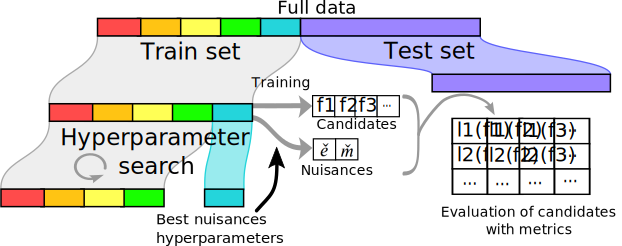
\includegraphics[width=\linewidth]{img/chapter_5/estimation_procedure_causal_selection_procedure.png}
    \caption{Estimation procedure for causal model
      selection.}\label{problem:estimation_procedure:figure}
  \end{figure}
\end{minipage}



\section{Theory: Links between feasible and oracle risks}\label{sec:theory}

We now relate two feasible risks, $\mu \text{-risk}_{IPW}$ and the
$R\text{-risk}$ to the oracle $\tau\text{-risk}$. Both results make
explicit the role of overlap for the performances of causal risks.

These bounds depend on a specific form of residual that we now define: for each potential outcome, $a \in  \{0; 1\}$, the variance conditionally on $x$
is \citep{shalit_estimating_2017}:
\begin{equation*}\label{eq:residuals}
  \sigma_{y}^{2}(x ; a) \overset{\text{def}}{=}
  \int_{y}\left(y-\mu_{a}(x)\right)^{2} p(y \mid x=x ; A=a) \, d y
\end{equation*}
Integrating over the population, we get the Bayes squared error:
$\sigma^2_{B}(a) = \int_{\mathcal X} \sigma_y^2(x;a) p(x)dx$
and its propensity weighted version:
$\tilde{\sigma}^2_{B}(a) = \int_{\mathcal X}\sigma_y^2(x;a)\,  p(x;
  a)\,dx$. In case of a purely deterministic link between the
covariates, the treatment, and the outcome, these residual terms are null.


\subsection{Upper bound of $\tau\text{-risk}$ with $\mu\text{-risk}_{IPW}$}%
\label{theory:mu_risk_ipw_bound}%

\begin{proposition}[Upper bound with $\mu \text{-risk}_{IPW}$
  ]\label{theory:prop:mu_risk_ipw_bound}
  \citep{johansson2022generalization} Given an outcome model $f$, let a
  weighting function $w(x; a) = \frac{a}{e(x)} + \frac{1-a}{1-e(x)}$ as the
  Inverse Propensity Weight. Then, under overlap (assumption
  \ref{assumption:overlap}), we have:
  \begin{equation*}
    \tau\text{-risk}(f) \leq \; 2 \, \mu\text{-risk}_{IPW}(w, f)
    - 2 \, \big(\sigma^2_{B}(1) +  \sigma^2_{B}(0)\big)
  \end{equation*}
\end{proposition}
This result has been derived in previous work
\citep{johansson2022generalization}. It links $\mu\text{-risk}_{IPW}$ to
the squared residuals of each population. For completeness, we provide the proof in \ref{apd:proofs}.

The upper-bound comes from the triangular inequality applied to the residuals of
both populations. The two quantities are equal when the
absolute residuals on treated and untreated populations are equal on the
whole covariate space:
$\forall x \in \mathcal X, |\mu_1(x) - f(x, 1)| = |\mu_0(x) - f(x, 0)|$.
The main difference between the oracle $\tau \text{-risk}$ and the
reweighted mean squared error, $\mu\text{-risk}_{IPW}$, comes from heterogeneous
residuals between populations.
% These quantities are difficult to characterize as
%they are linked both to the estimator and to the data distribution.
%
This bound shows that minimizing the $\mu\text{-risk}_{IPW}$ helps to
minimize the $\tau\text{-risk}$, which leads to
interesting optimization procedures \citep{johansson2022generalization}. However, there is no
guarantee that this bound is tight, which makes it fragile for model
selection.

Assuming strict overlap (probability of all individuals being treated or not
bounded away from 0 and 1 by $\eta$, \ref{background:causal_assumptions}), the
above bound simplifies into a looser one involving the usual mean squared error:
$\tau\text{-risk}(f)\leq \frac{2}{\eta}\, \mu\text{-risk}(f) -  2 \, \big(\sigma^2_{B}(1) +  \sigma^2_{B}(0)\big)$. For weak overlap (propensity scores not bounded far from 0
or 1), this bound is very loose (as shown in Figure \ref{fig:toy_example})
and is not appropriate to discriminate between models with close performances.

%\md{Lower bound: I think that there is no lower bound of the tau-risk with the
%mu-risk. That means that we can have a mu risk of 0 wheras the taurisk is
%non-null. Todo for myself: develop an example with overfitted 1NN on the
%observed data.}

\subsection{Reformulation of the $R\text{-risk}$ as reweighted $\tau\text{-risk}$}%
\label{theory:r_risk_rewrite}%

We now derive a novel rewriting of the $R\text{-risk}$, making explicit its link
with the oracle $\tau \text{-risk}$.

\begin{proposition}[$R \text{-risk}$ as reweighted
    $\tau\text{-risk}$]\label{theory:prop:r_risk_rewrite} Given an outcome model
  $f$, its $R\text{-risk}$ appears as weighted version of its $\tau\text{-risk}$
  (Proof in \ref{apd:proofs:r_risk_rewrite}):
  \begin{align}
    R\text{-risk}^*(f) & = \int_{x} e(x)\big(1-e(x)\big)\big(\tau(x)-\tau_ {f}(x)\big)^{2} p(x) d x  \quad\; + \tilde{\sigma}_B^2(1) + \tilde{\sigma}_B^{2}(0)
  \end{align}
\end{proposition}

The $R \text{-risk}$ targets the oracle at the cost of an overlap re-weighting
and the addition of the reweighted Bayes residuals, which are independent of
$f$. In good overlap regions the weights $e(x) \big(1-e(x) \big)$ are close to
$\frac{1}{4}$, hence the $R \text{-risk}$ is close to the desired gold-standard
$\tau \text{-risk}$. On the contrary, for units with extreme overlap violation,
these weights go down to zero with the propensity score.

% \begin{remark}[Trivial upper bound] Because $e(x)\leq1$ and $(1-e(x))\leq1$,
%   we see immediately that \begin{equation} R \text{-risk}^* \leqslant
%   \tau{\text{-risk}}+\tilde{\sigma_{B}}(1)^{2}+\tilde{\sigma_{B}}^{2}(0)
%   \end{equation} \end{remark}

% \begin{remark}[Lower bound] Due to strict overlap assumption, \begin{equation}
%   R \text{-risk}^* \geqslant \eta (1 - \eta)
%   \tau{\text{-risk}}-\tilde{\sigma_{B}}(1)^{2}-\tilde{\sigma_{B}}^{2}(0)
%   \end{equation} \end{remark}

% \begin{remark}[Cases of loose upper bounds] Giving a strict overlap assumption
%   $\eta$, we can exhibit for all $C \; st. \; \eta^{-1}>C>1$, simple
%   simulations where: \begin{equation} R \text{-risk}^* \leqslant C \; \eta \;
%   \tau \text{-risk}(f) \quad \end{equation} \end{remark}

\subsection{Interesting special cases}

\paragraph{Randomization special case}\label{remark:rct} If the treatment is
randomized as in RCTs, $p(A=1 \mid X=x) = p(A=1)=p_A$, thus
$\mu\text{-risk}_{IPW}$ takes a simpler form:
\begin{equation*}
  \mu\text{-risk}_{IPW} = \mathbb{E}_{(Y, X, A) \sim \mathcal D}\left[ \Big( \frac{A}{p_A} + \frac{1-A}{1-p_A} \Big) (Y-f(X ; A))^2 \right]
\end{equation*}
However, we still can have large differences
between $\tau\text{-risk}$ and $\mu\text{-risk}_{IPW}$ coming from heterogeneous
errors between populations as noted in Section \ref{theory:mu_risk_ipw_bound}
and shown experimentally in \citet{schuler_comparison_2018} and our
results below.

Concerning the $R\text{-risk}$, replacing $e(x)$ by its randomized value $p_A$
in Proposition \ref{theory:prop:r_risk_rewrite} yields the oracle
$\tau\text{-risk}$ up to multiplicative and additive constants:
\begin{equation*}
  R\text{-risk} = p_A \, (1-p_A) \, \tau\text{-risk} \;+\; (1 - p_A) \,\sigma_B^2(0) \;+\; p_A \sigma_B^2(1)
\end{equation*}
Thus, selecting estimators with $R\text{-risk}^*$ in
randomized setting controls the $\tau\text{-risk}$. This explains
the strong performances of $R\text{-risk}$ in randomized setups
\citep{schuler_comparison_2018} and is a strong argument to use it
to estimate heterogeneity in RCTs.

\paragraph{Oracle Bayes predictor}\label{remark:bayes_oracle} If we
have access to the oracle Bayes predictor for the outcome ie.~$f(x,
  a)=\mu(x, a)$, then all risks are equivalent up to the residual variance:
\begin{equation}
  \tau\text{-risk}(\mu) = \mathbb E_{X\sim p(X)}[(\tau(X) - \tau_{\mu}(X))^2] = 0
\end{equation}
\begin{align}
  \mu\text{-risk}(\mu) & = \mathbb E_{(Y, X, A) \sim p(Y;X;A)}[\big( Y - \mu_A(X)\big)^2]
  = \int_{\mathcal X, \mathcal A}
  \,\varepsilon(x,a)^2 p(a \mid x) \,p(x) \,dx\,da  \leq \sigma_B^{2}(0) + \sigma_B^{2}(1)
\end{align}
\begin{equation}
  \mu\text{-risk}_{IPW}(\mu) = \sigma_B^{2}(0) + \sigma_B^{2}(1)  \quad \text{from Lemma \ref{apd:proofs:mu_risk_ipw_link_mu}}
\end{equation}
\begin{equation}
  R\text{-risk}(\mu) = \tilde{\sigma}_B^{2}(0) + \tilde{\sigma}_B^{2}(1)
  \leq \sigma_B^{2}(0) + \sigma_B^{2}(1)  \quad  \text{from Proposition \ref{theory:prop:r_risk_rewrite}}%\notag
\end{equation}

Thus, differences between causal risks only matter in finite sample regimes.
Universally consistent learners converge to the Bayes risk in asymptotic
regimes, making all model selection risks equivalent. In practice however,
choices must be made in non-asymptotic regimes.



\section{Empirical Study}\label{sec:empirical_study}

%We now explore empirically the behavior of these different causal selection
%metrics.
%\subsection{Causal metrics under evaluation}

We evaluate the following causal metrics, oracle and feasible
versions, presented in Table
\ref{tab:evaluation_metrics}:\\
$\widehat{\mu\text{-risk}}_{IPW}^*$,
$\widehat{R\text{-risk}}^*$,
$\widehat{U\text{-risk}}^*$,
$\widehat{\tau\text{-risk}_{IPW}}^*$,
$\widehat{\mu\text{-risk}}$,
$\widehat{\mu\text{-risk}}_{IPW}$,
$\widehat{R\text{-risk}}$,
$\widehat{U\text{-risk}}$,
$\widehat{\tau\text{-risk}_{IPW}}$.
We benchmark the metrics in a variety of settings:
many different simulated data generation
processes and three semi-simulated datasets \footnote{Scripts for the simulations and the selection procedure are available at
  \url{https://github.com/soda-inria/caussim}.
}.

\subsection{Caussim: Extensive simulation settings}\label{subsec:simulations}

\paragraph{Data Generation}

We use simulated data, on which the ground-truth causal effect is known. Going
beyond prior empirical studies of causal model selection
\citep{schuler_comparison_2018,alaa_validating_2019}, we use many
generative processes, to reach more general conclusions (as discussed
in \ref{apd:results:fig:seed_effect}).

We generate the response functions using random bases. Basis extension methods
are common in biostatistics, \emph{eg} functional regression with splines
\citep{howe_splines_2011, perperoglou_review_2019}. By allowing the function to
vary at specific knots, they give flexible non-linear models. We use random approximation of Radial Basis Function (RBF) kernels
\citep{rahimi_random_2008} to generate the response functions. RBF use the same
process as polynomial splines but replace polynomial by Gaussian kernels. Unlike
polynomials, Gaussian kernels have decreasing influences in the input space.
This avoids unrealistic divergences of the response surfaces at the
ends of the feature space.

The number of basis functions --\emph{ie. knots}--, controls the complexity of
the ground-truth response surfaces and treatment. We first use this process to
draw the non-treated response surface $\mu_0$ and the causal effect $\tau$. We
then draw the observations from a mixture two Gaussians, for the treated and non
treated. We vary the separation between the two Gaussians to control the
overlap between treated and non-treated populations, an important parameter
for causal inference (related to $\eta$ in section
\ref{theory:mu_risk_ipw_bound}). Finally, we generate observed outcomes
adding Gaussian noise yielding a dataset as plotted in Figure \ref{fig:simulation_examples}. We generate 1\,000 of such datasets, with
uniformly random overlap parameters. Details in
\ref{apd:experiments:generation}.

\captionsetup[sub]{font=large,labelfont={bf,sf}}%

\begin{figure}[b!]
  \begin{minipage}{0.3\textwidth}
    \caption{Example of the simulation setup in the input space with two
      knots --\emph{ie.}basis functions. The top panel
      shows the observations in feature space, while the bottom panel displays the
      two response surfaces on a 1D cut along the black lines drawn on
      the top panel.}
    \label{fig:simulation_examples}
  \end{minipage}
  \hfill
  \begin{minipage}{0.65\textwidth}
    \centering
    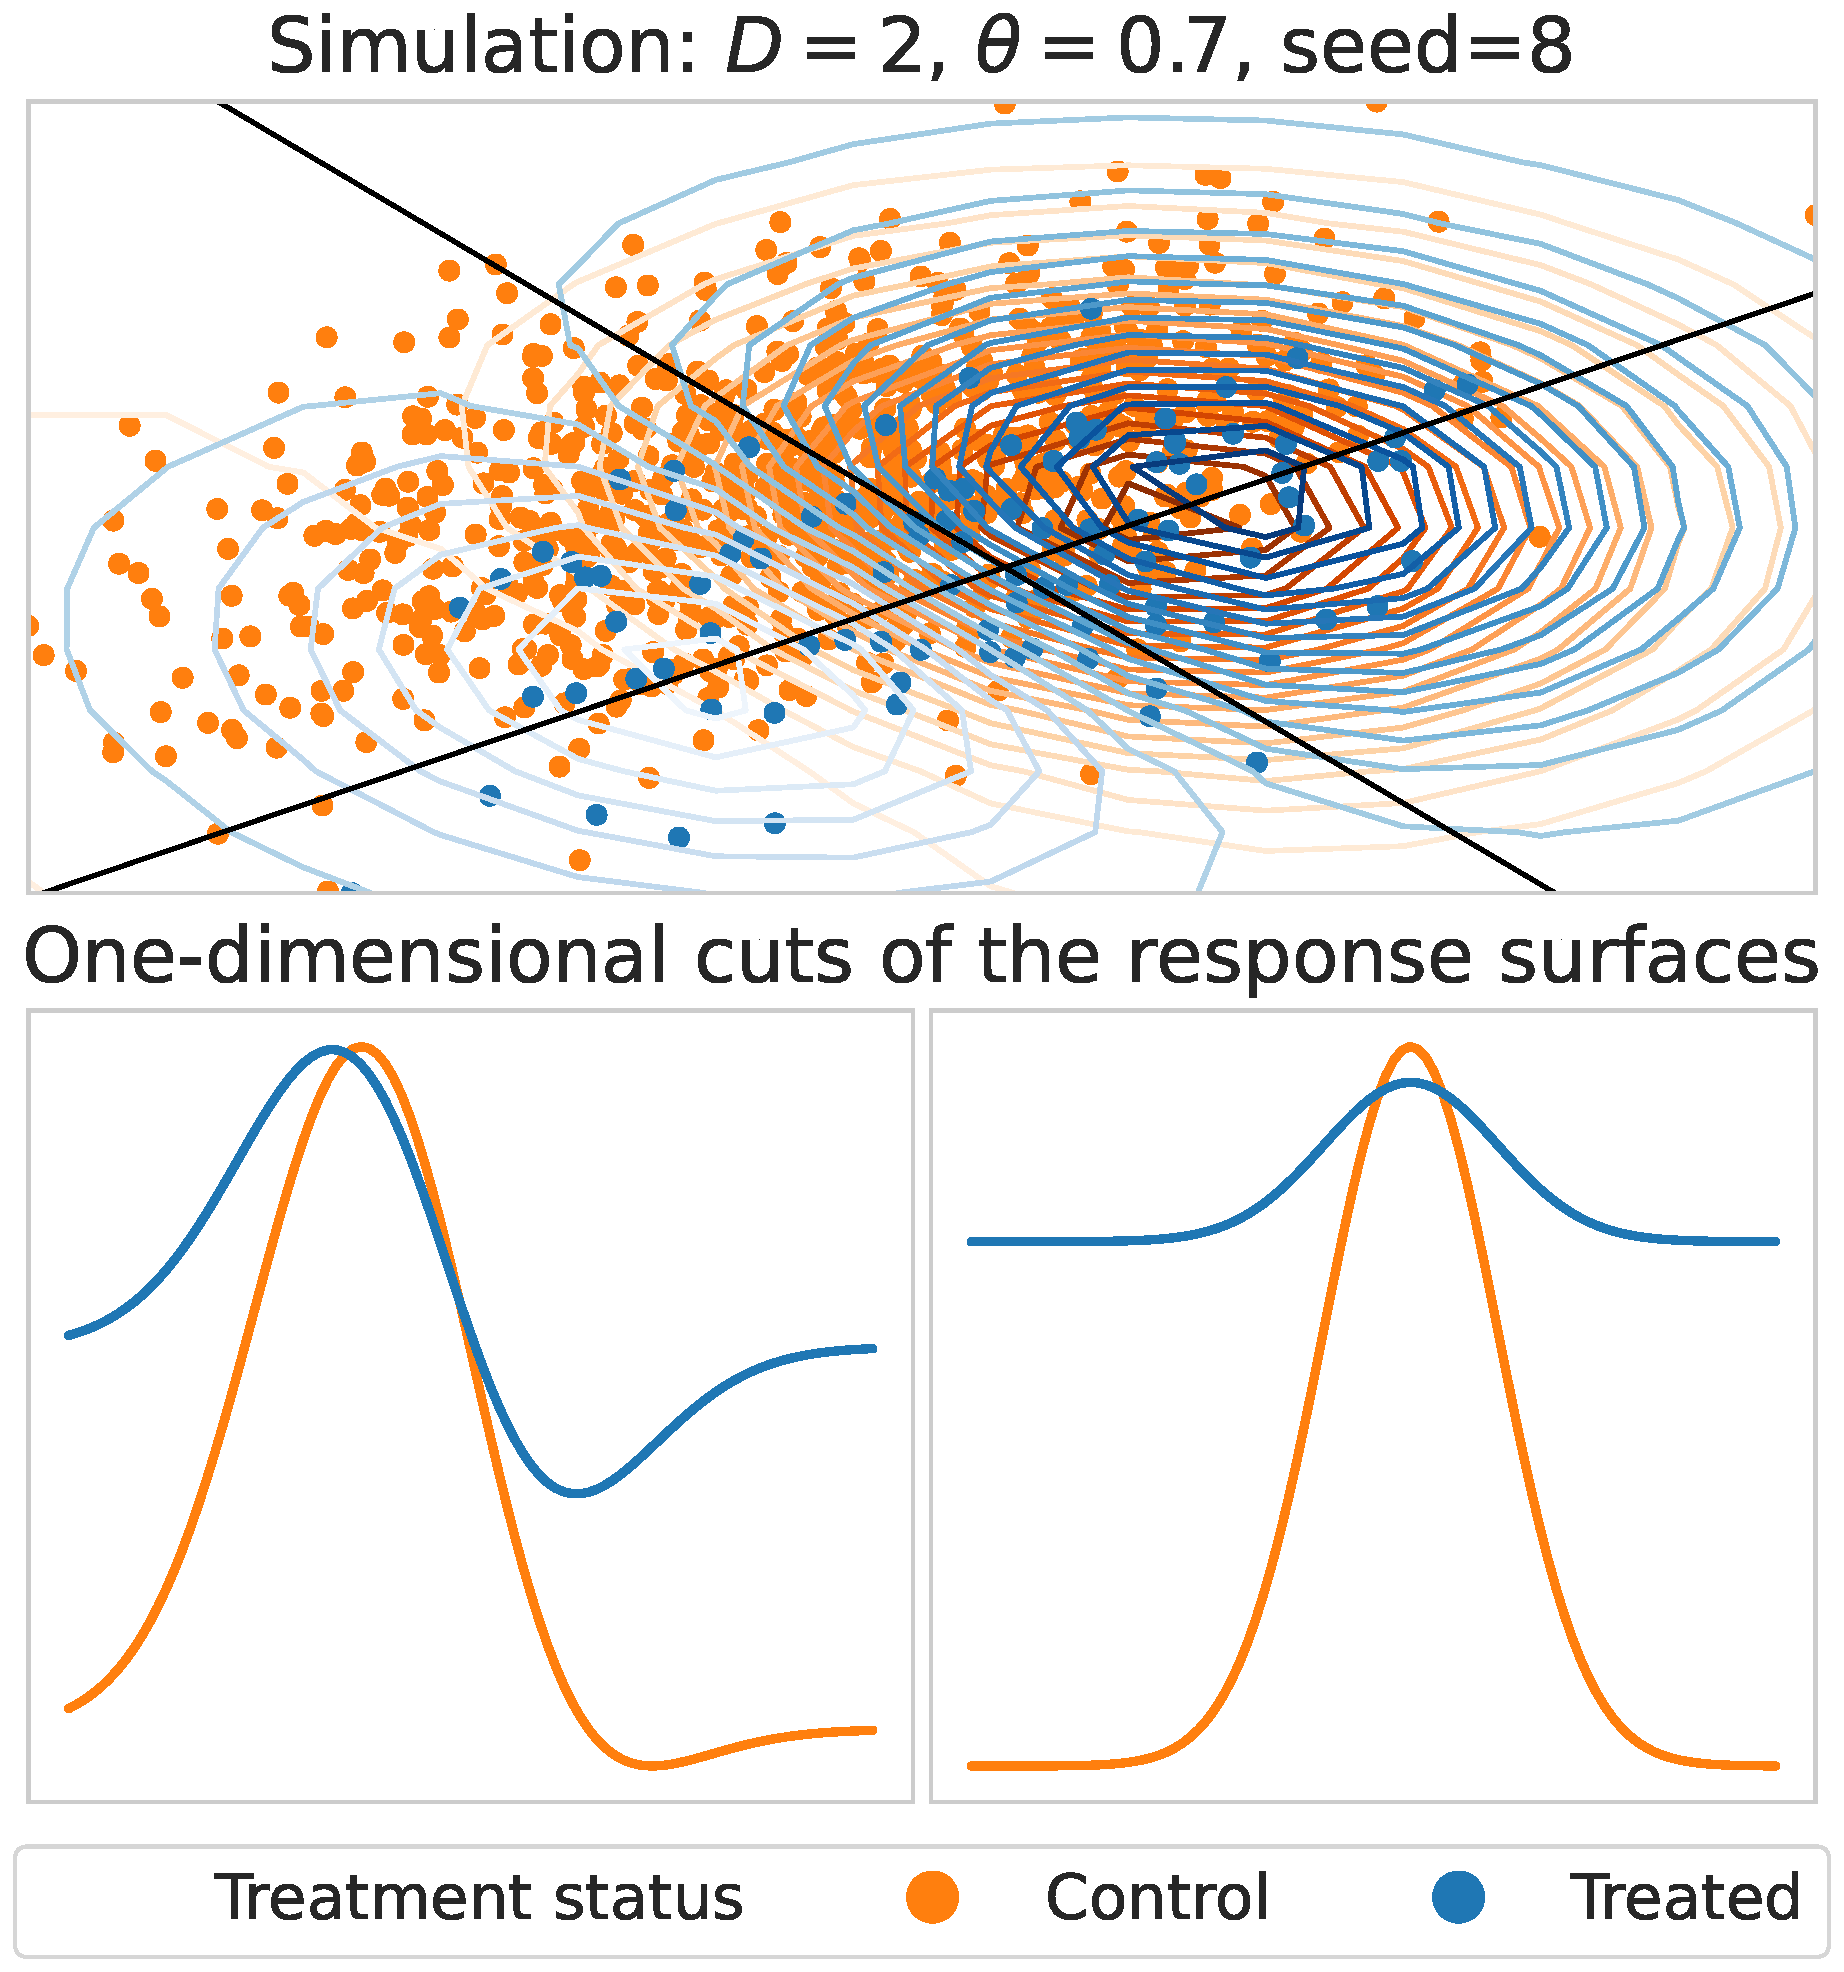
\includegraphics[width=0.8\linewidth]{img/chapter_5/caussim_example_rs_gaussian=8_rs_rotation=8_ntv=0.37_D=2_overlap=0.7_p_A=0.1.pdf}
  \end{minipage}
\end{figure}


\paragraph{Family of candidate estimators}

We test model selection on a family of candidate estimators that
approximate imperfectly the data-generating process. To build such an
estimator, we first use a RBF expansion
similar to the one used for data generation.
We choose two random knots and apply a transformation of the raw data features
with a Gaussian kernel. This step
is referred as the featurization. Then, we fit a linear regression on
these
transformed features. We consider two ways of combining these steps for outcome
mode; we use common nomenclature \citep{kunzel_metalearners_2019,shen2023rctrep} to refer
to these different meta-learners that differ on how
they model, jointly or not, the treated and the non treated:
\begin{itemize}
  \item SLearner: A single learner for both population, taking the treatment as
        a supplementary covariate.

  \item SftLearner: A single set of basis functions is sampled at random for both
        populations, leading to a given feature space used to model both the treat and
        the non treated, then two
        separate different regressors are fitted on this shared representation.
  \item TLearner: Two completely different learners for each population, hence
        separate feature representations and regressors.
\end{itemize}

We do not include more elaborated meta-learners such as R-learner
\citep{nie_quasioracle_2017} or X-learner
\citep{kunzel_metalearners_2019}. Our goal is not to have the best possible
learner but to have a variety of sub-optimal learners to compare the
different causal metrics. For the same reason, we did not include more powerful
outcome models such as random forests or boosting trees.

For the regression step, we fit a Ridge regression on the transformed features
with 6 different choices of the regularization parameter $\lambda \in [10^{-3},
    10^{-2}, 10^{-1}, 1, 10^{1}, 10^{2}]$, coupled with a TLearner or a SftLearner.
We sample 10 different random basis for learning and
featurization yielding a family $\mathcal F$ of 120 candidate estimators.
%

\subsection{Semi-simulated datasets}\label{subsec:causal_model_selection:semi_simulated}

\paragraph{Datasets}

We also use classic benchmarks of the causal-inference
literature, semi-simulated data adding a known synthetic causal effect to real --non synthetic-- covariate:
\begin{description}
  \item[ACIC 2016] \citep{dorie_automated_2019}: The dataset is based on the
    Collaborative Perinatal Project \citep{niswander_women_1972}, a RCT
    studying infants’
    developmental disorders. The initial intervention was a child’s birth
    weight $(A = 1 \text{ if weight} < 2.5 kg)$, and outcome was the child’s
    IQ after a follow-up period. The study contained $N=4\,802$ data
    points with $D=55$ features (5 binary, 27 count data, and 23
    continuous). They simulated 77 different setups varying parameters
    for treatment and response models, overlap, and interactions between treatment and
    covariates \footnote{Original R code available at
      \url{https://github.com/vdorie/aciccomp/tree/master/2016}
      to generate 77 simulations settings.}. We used 10 different seeds for
    each setup, totaling 770 dataset instances.

  \item[ACIC 2018] \citep{shimoni_benchmarking_2018}: Starting from data
    from the Linked Births and Infant Deaths Database (LBIDD)
    \citep{macdorman_infant_1998} with $D=177$ covariates, treatment and
    outcome models are simulated with complex models to reflect
    different scenarii. The data do not provide the true propensity
    scores, so we evaluate only feasible metrics, which do not require this
    nuisance parameter. We used all 432 datasets\footnote{Using the scaling part of the data, from
      \href{https://github.com/IBM-HRL-MLHLS/IBM-Causal-Inference-Benchmarking-Framework}{github.com/IBM-HRL-MLHLS/IBM-Causal-Inference-Benchmarking-Framework}} of size $N=5\,000$.


  \item[Twins] \citep{louizos_causal_2017}: It is an augmentation of
    real data on twin births and mortality rates
    \citep{almond_costs_2005}. There are $N=11\,984$ samples (pairs of twins),
    and $D=50$ covariates\footnote{We obtained the dataset from
      \href{https://github.com/AMLab-Amsterdam/CEVAE/tree/master/datasets/TWINS}{https://github.com/AMLab-Amsterdam/CEVAE/tree/master/datasets/TWINS}}, The outcome is the mortality and the treatment is the
    weight of the heavier twin at birth. This is a "true" counterfactual dataset
    \citep{curth_really_2021} in the sense that we have
    both potential outcomes with each twin. They simulate the treatment with a
    sigmoid model based on GESTAT10 (number of gestation weeks before birth) and x
    the 45 other covariates:
    \begin{align}
      \mathbf{t}_{i} & \mid \mathbf{x}_{i}, \mathbf{z}_{i} \sim
      \operatorname{Bern}\left(\sigma\left(w_{o}^{\top}
      \mathbf{x}+w_{h}(\mathbf{z} / 10-0.1)\right)\right)       \\ & \text{with} \;
      w_{o} \sim \mathcal{N}(0,0.1 \cdot I),\; w_{h} \sim \mathcal{N}(5,0.1) \nonumber
    \end{align}
    We add a non-constant slope in the
    sigmoid to control the overlap between
    treated and control populations.
    We sampled uniformly 1\,000 different overlap parameters between 0 and
    2.5, totaling 1\,000 dataset instances. Unlike the previous datasets,
    only the overlap varies for these instances. The response surfaces are
    set by the original outcomes.
\end{description}

\paragraph{Family of candidate estimators}

For these three datasets, the family of candidate estimators are gradient
boosting trees for both the response surfaces and the treatment
\footnote{Scikit-learn regressor,
  \href{https://scikit-learn.org/stable/modules/generated/sklearn.ensemble.HistGradientBoostingRegressor.html}{HistGradientBoostingRegressor},
  and classifier,
  \href{https://scikit-learn.org/stable/modules/generated/sklearn.ensemble.HistGradientBoostingClassifier.html}{HistGradientBoostingClassifier}.}
with S-learner, learning rate
in $\{0.01, 0.1, 1\}$, and maximum number of leaf nodes in $\{25, 27, 30, 32,
  35, 40\}$ resulting in a family of size 18.

\paragraph{Nuisance estimators}

Drawing inspiration from the TMLE literature that uses combination of flexible
machine learning methods \citep{schuler_targeted_2017}, we use as models
for the nuisances $\check e$ (respectively $\check m$) a form of meta-learner: a
stacked estimator of ridge and boosting classifiers (respectively
regressions). We select hyper-parameters with randomized search on a validation set
$\mathcal{V}$ and keep them fix for model selection
(\ref{apd:experiments:nuisances_hp} lists hyperparameters). As extreme inverse
propensity weights induce high variance, we use clipping
\citep{swaminathan_counterfactual_2015, ionides_truncated_2008} to bound
$min(\check e, 1-\check e)$ away from 0 with a fixed $\eta=10^{-10}$, ensuring
strict overlap for numerical stability.


%\paragraph{Model selection procedure}\label{semi_simulated:selection_procedure}

%We used the same training procedure procedure as in
%\ref{paragraph:selection_procedure} (Details in supp.~mat.
%\ref{apd:selection_procedure_acic}).

\subsection{Measuring overlap between treated and non treated}%
\label{subsec:causal_model_selection:measuring_overlap}%

%\idea{Overlap is important but not easily measurable}
Good overlap between treated and control population is
crucial for causal inference as it is required by the positivity assumption
\ref{assumption:overlap}. It is often assessed by
comparing visually population distributions (as in Figure
\ref{fig:toy_example}) or computing standardized difference on each
feature
\citep{austin_introduction_2011,austin_moving_2015}. While these methods are
useful to decide if positivity holds, they do not yield a
single measure. Rather, we compute the divergence
between the population covariate distributions $\mathbb P(X|A=0)$ and $\mathbb
  P(X|A=1)$
\citep{damour_overlap_2020,johansson2022generalization}. We introduce the
Normalized Total Variation (NTV), a divergence based on the sole propensity
score (see \ref{apd:motivation_ntv}).

\begin{figure}[!b]
  \centering
  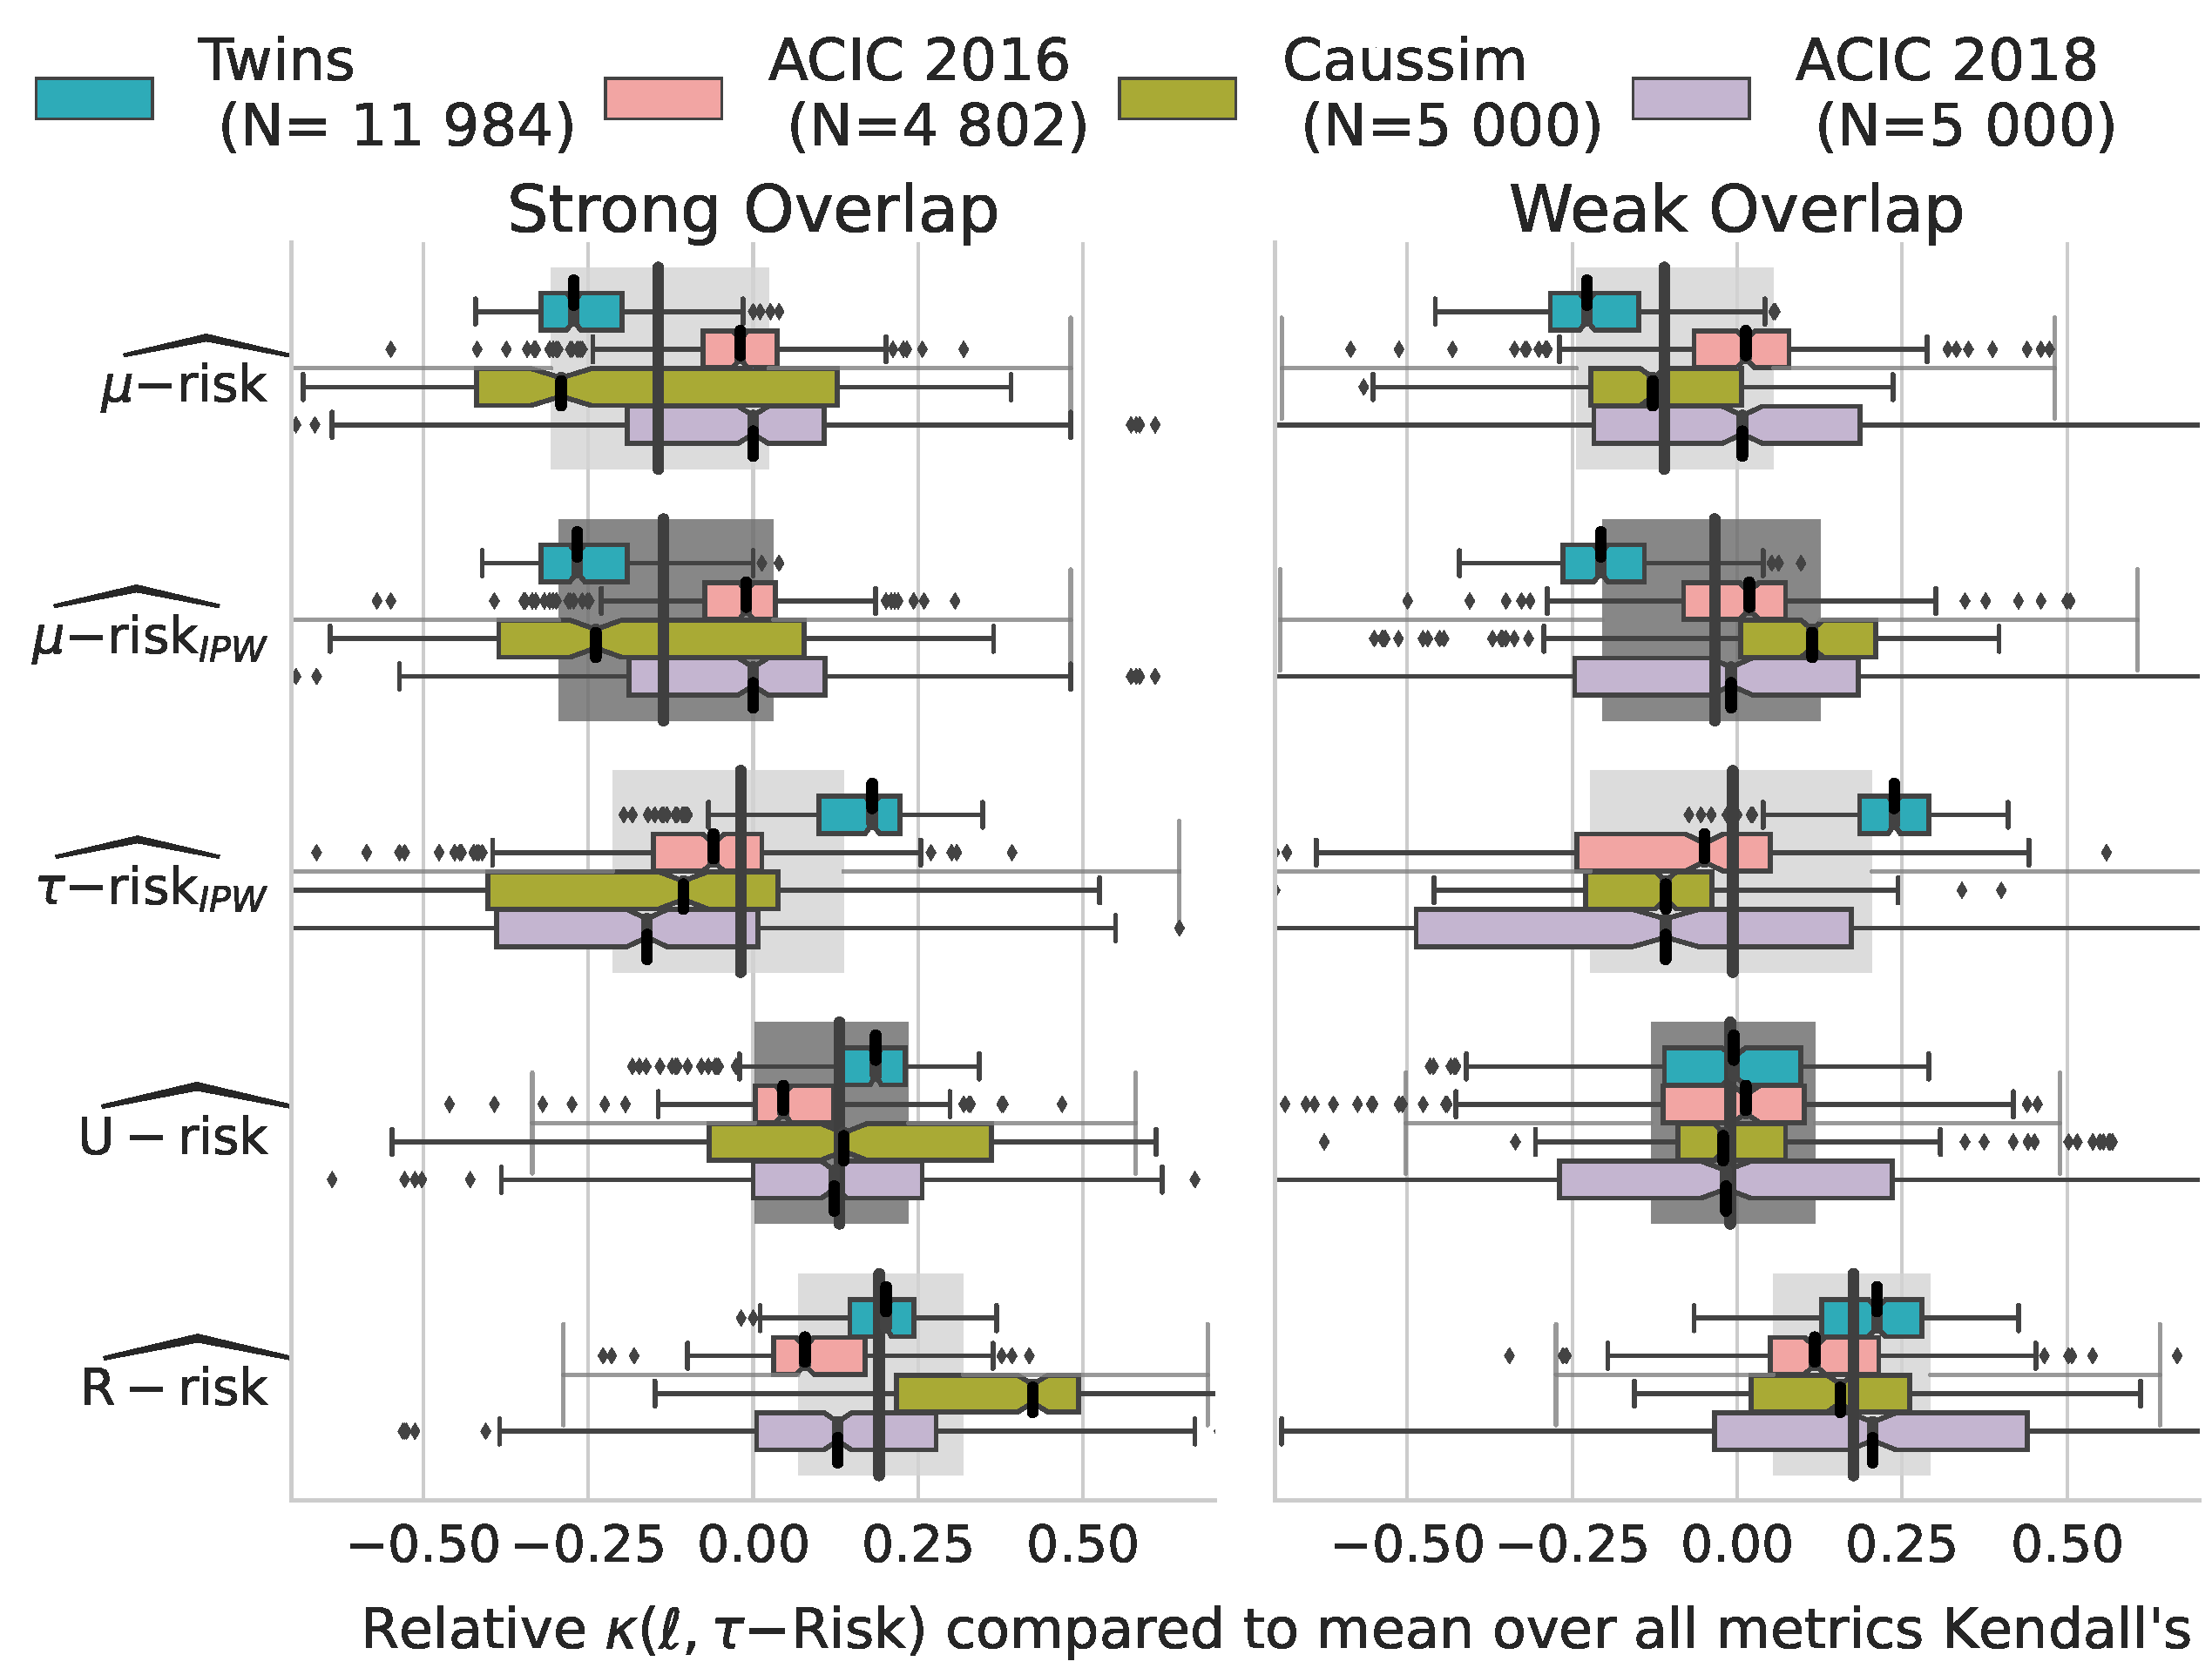
\includegraphics[width=0.9\linewidth]{img/chapter_5/_1_r_risk_domination_r_risk_domination__ref_metric_mean_risks_by_Dataset_feasible_only.pdf}
  %\hfill
  \caption{\textbf{The $R$-risk is the best metric}: Relative Kendall's $\tau$ agreement with $\tau\text{-risk}$.
    Strong and Weak overlap correspond to the first and last tertiles of the overlap distribution measured with
    Normalized Total Variation eq. \ref{eq:ntv}. \ref{apd:experiments:additional_results} presents the same results
    by adding semi-oracle risks in Figure \ref{apd:fig:relative_kendalls_all_datasets_all_metrics}, measured with
    absolute Kendall's in Figure \ref{apd:fig:all_datasets_tau_risk_ranking_agreement} and with $\tau\mathrm{-risk}$
    gains in Figure \ref{apd:all_datasets_normalized_bias_tau_risk_to_best_method}. Table
    \ref{apd:table:relative_kendalls_all_datasets} gives median and
    IQR of the relative Kendall.}\label{fig:relative_kendalls_all_datasets}
\end{figure}

\subsection{Results: factors driving good model selection}%
\label{subsec:causal_model_selection:empirical_results}%

\paragraph{The $R\text{-risk}$ is the best metric}

Each metric ranks differently the candidate models. Figure
\ref{fig:relative_kendalls_all_datasets} shows the agreement between the
ideal ranking of methods given the oracle $\tau\text{-risk}$ and
the different feasible causal metrics. We measure this agreement
with a relative\footnote{To remove the variance
  across datasets (some datasets lead to easier model selection than
  others), we report values for one metric relative to the mean of all
  metrics for a given dataset instance: $\text{Relative} \, \kappa(\ell,\tau\mathrm{{-risk}})=
    \kappa(\ell,\tau\mathrm{{-risk}}) -
    mean_{\ell}\big(\kappa(\ell,\tau\mathrm{{-risk}})\big)$} Kendall tau $\kappa$ (eq.
\ref{eq:kendall_tau}) \citep{kendall_new_1938}.
Given the importance of overlap in
how well metrics approximate the oracle $\tau\text{-risk}$
(\ref{apd:proofs:mu_risk_ipw_bound}), we separate
strong and weak overlap.

Among all metrics, the classical mean squared error (ie. factual
$\mu\text{-risk}$) is worse and reweighting it with propensity score
($\mu\text{-risk}_{IPW}$) does not bring much improvements. The
$R\text{-risk}$, which includes a model of mean outcome and propensity
scores, leads to the best performances. Interestingly, the
$U\text{-risk}$, which uses the same nuisances, deteriorates in weak overlap, probably due to variance
inflation when dividing by extreme propensity scores.

Beyond rankings, the differences in terms of absolute
ability to select the best model are large: The R-risk selects a model
with a $\tau\text{-risk}$ only 1\% higher
than the best
possible candidate for strong overlap on Caussim, but selecting with
the $\mu\text{-risk}$ or $\mu\text{-risk}_{IPW}$ --as per machine-learning
practice-- leads to 10\% excess risk and using $\tau\text{-risk}_{IPW}$
--as in some causal-inference methods \citep{athey2016recursive,gutierrez_causal_2016}--leads to 100\% excess risk
(Figure
\ref{apd:all_datasets_normalized_bias_tau_risk_to_best_method}). Across
datasets, the $R\text{-risk}$ consistently decreases the
risk compared to the $\mu\text{-risk}$:
0.1\% compared to 1\% on ACIC2016,  1\% compared to 20\% on ACIC2018,
and 0.05\% compared to 1\% on Twins.


\paragraph{Model selection is harder for low population
  overlap}

Model selection for
causal inference becomes more and more difficult with increasingly different
treated and control populations
(Figure \ref{fig:all_datasets_overlap_effect_r_risk}). The
absolute Kendall's coefficient correlation with $\tau\text{-risk}$
drops from values around 0.9 (excellent agreement with oracle selection) to 0.6 on
both Caussim and ACIC 2018
(\ref{apd:experiments:additional_results}).

\begin{figure}[h!]
  \begin{minipage}{.35\linewidth}
    \caption{\textbf{Model selection is harder for low population
        overlap}:
      Kendall's $\tau$ agreement with $\tau\text{-risk}$. Strong, medium and Weak overlap
      are the tertiles of the overlap measured with NTV eq. \ref{eq:ntv}. \ref{apd:experiments:additional_results} presents results for all
      metrics in Figure \ref{apd:fig:all_datasets_overlap_effect} in absolute
      Kendall's and continuous overlap values in Figure
        {\ref{apd:fig:all_datasets_tau_risk_ranking_agreement}}.}\label{fig:all_datasets_overlap_effect_r_risk}
  \end{minipage}
  \hfill
  \begin{minipage}{0.6\linewidth}
    \centering
    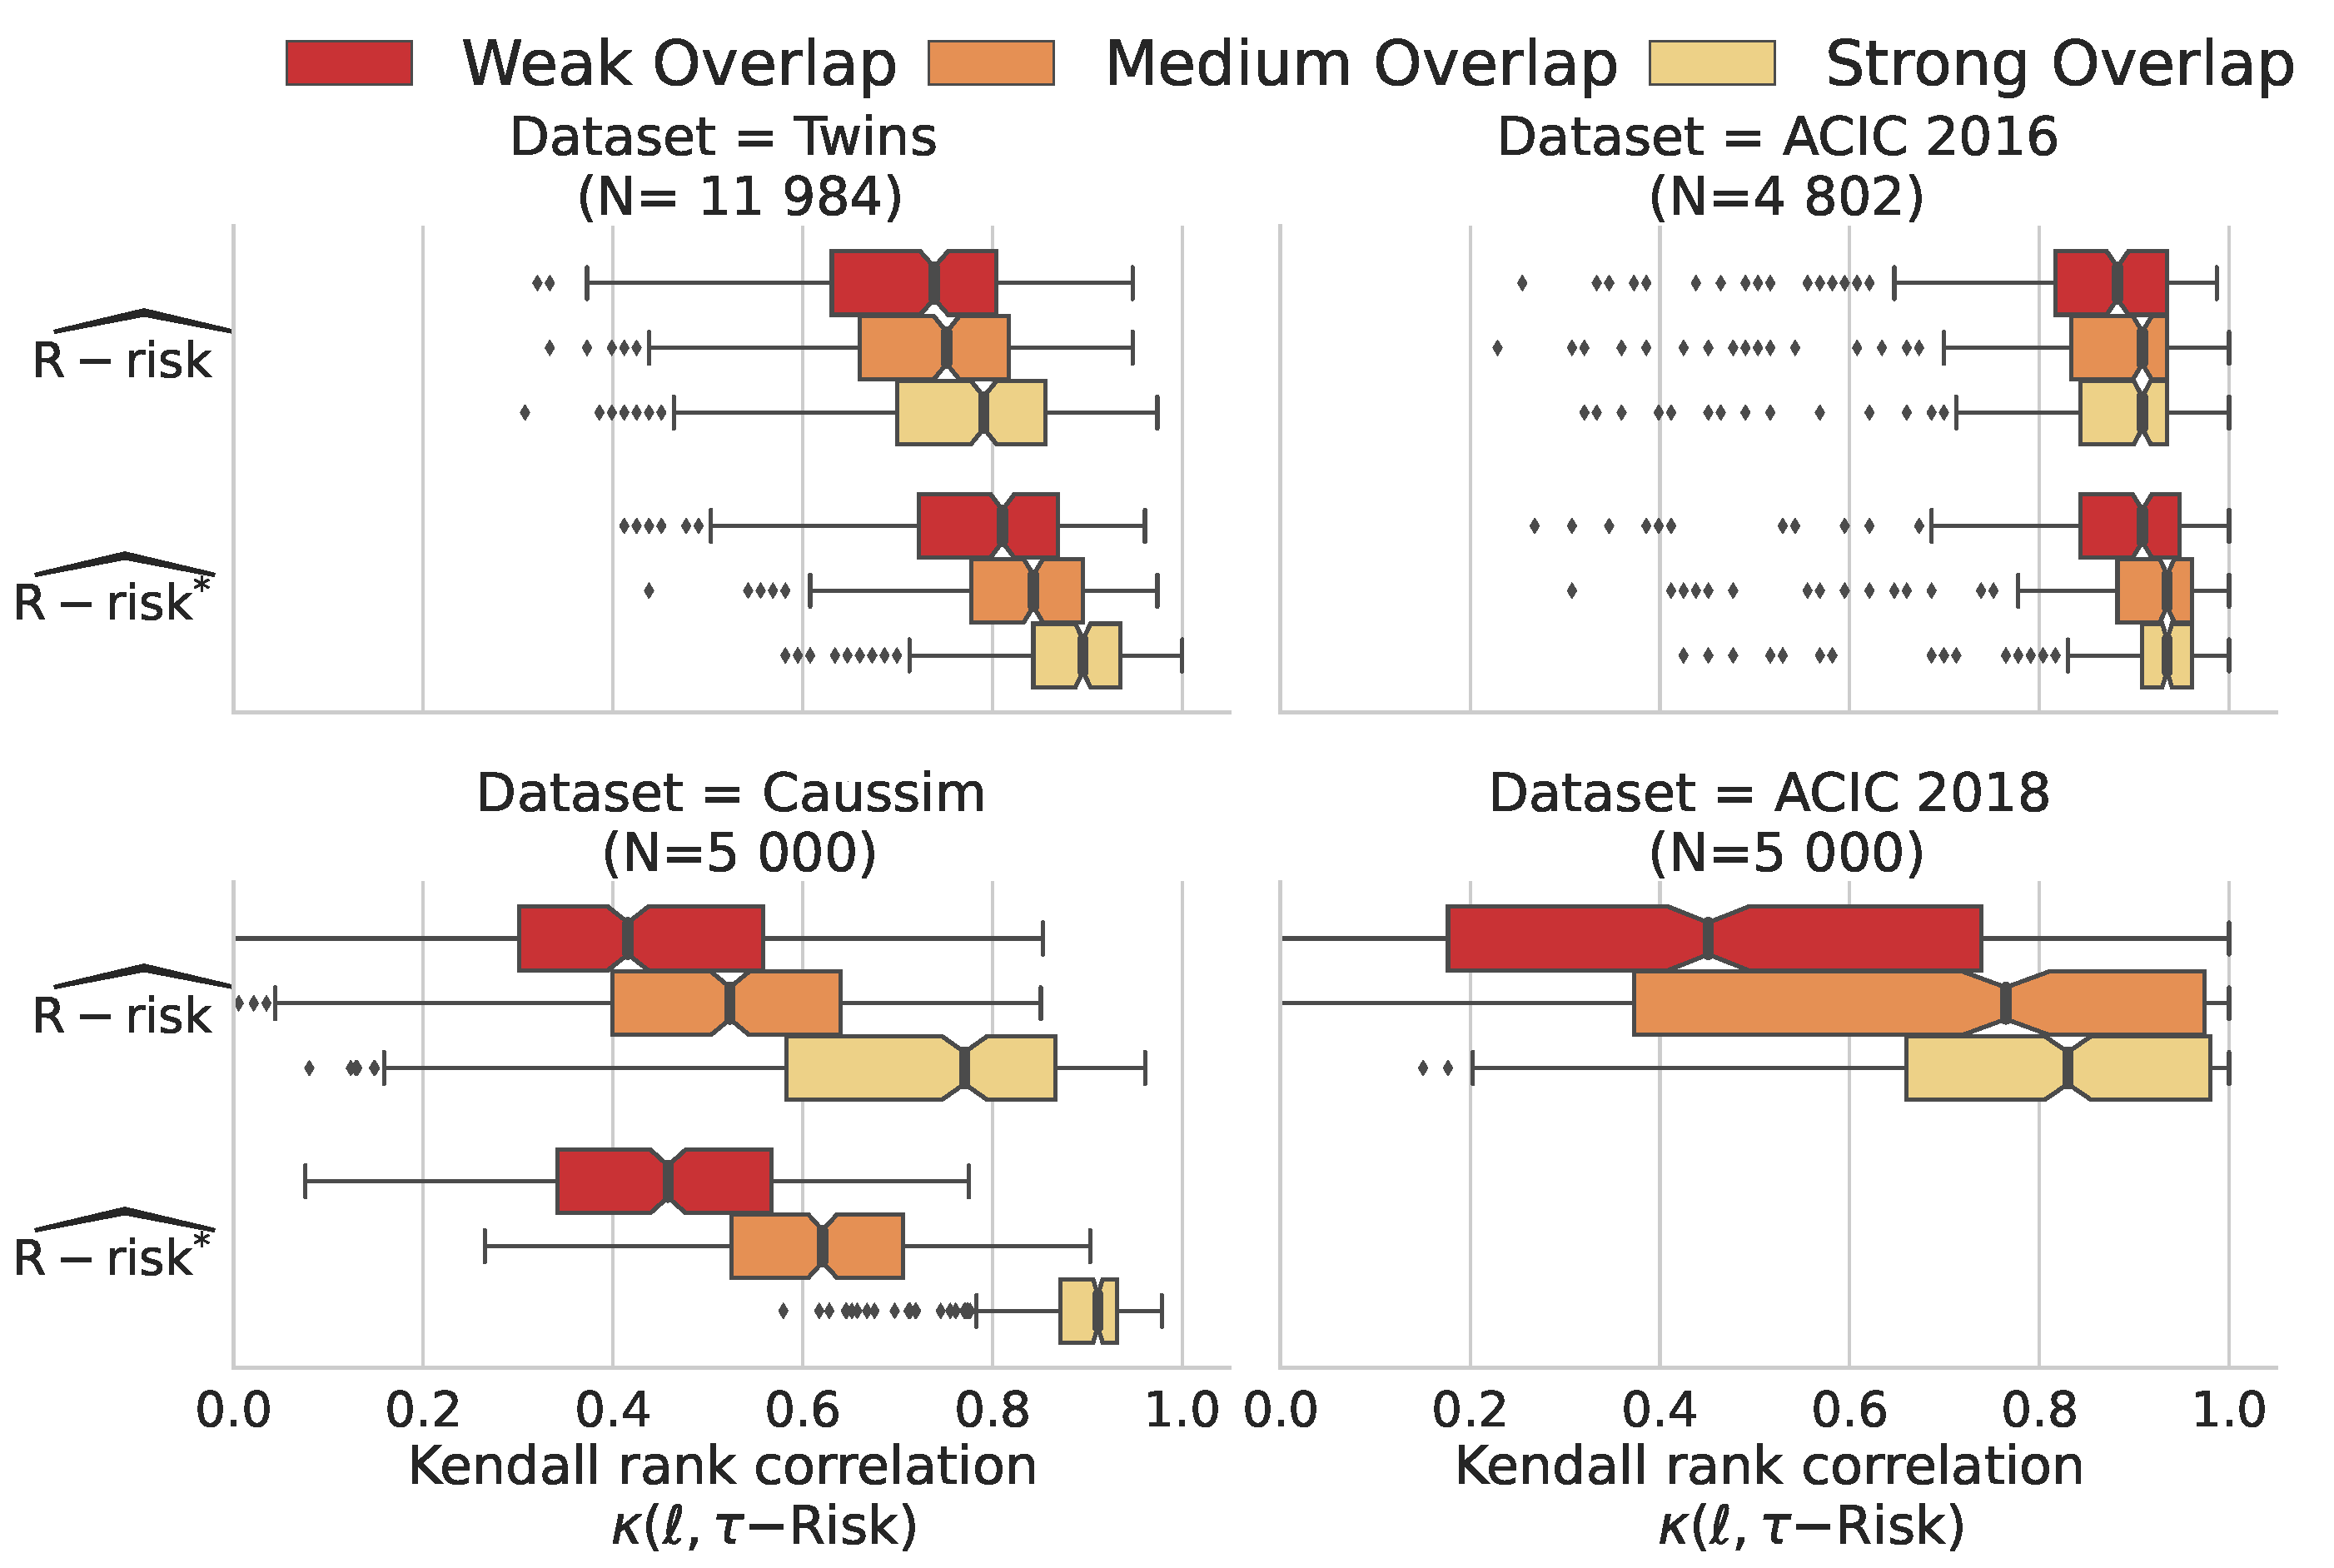
\includegraphics[width=\linewidth]{img/chapter_5/_2_overlap_influence_overlap_by_bin_comparaison_kendall_by_Dataset_r_risk_only.pdf}
  \end{minipage}
\end{figure}

\paragraph{Nuisances can be estimated on the same data as outcome models}

Using the train set $\mathcal{T}$ both to fit the candidate estimator and the
nuisance estimates is a form of double dipping which can lead errors in
nuisances correlated to that of outcome models
\citep{nie_quasioracle_2017}. In theory, these correlations can bias model
selection and, strictly speaking, push
to split out a third separated data set --a ``nuisance set''-- to fit the
nuisance models. The drawback is that it depletes the data available for
model estimation and selection. However, Figure
\ref{fig:procedures_comparison} shows no substantial difference between a procedure with a separated
nuisance set and the simpler shared nuisance-candidate set procedure.

\begin{figure}[!tb]
  \centering
  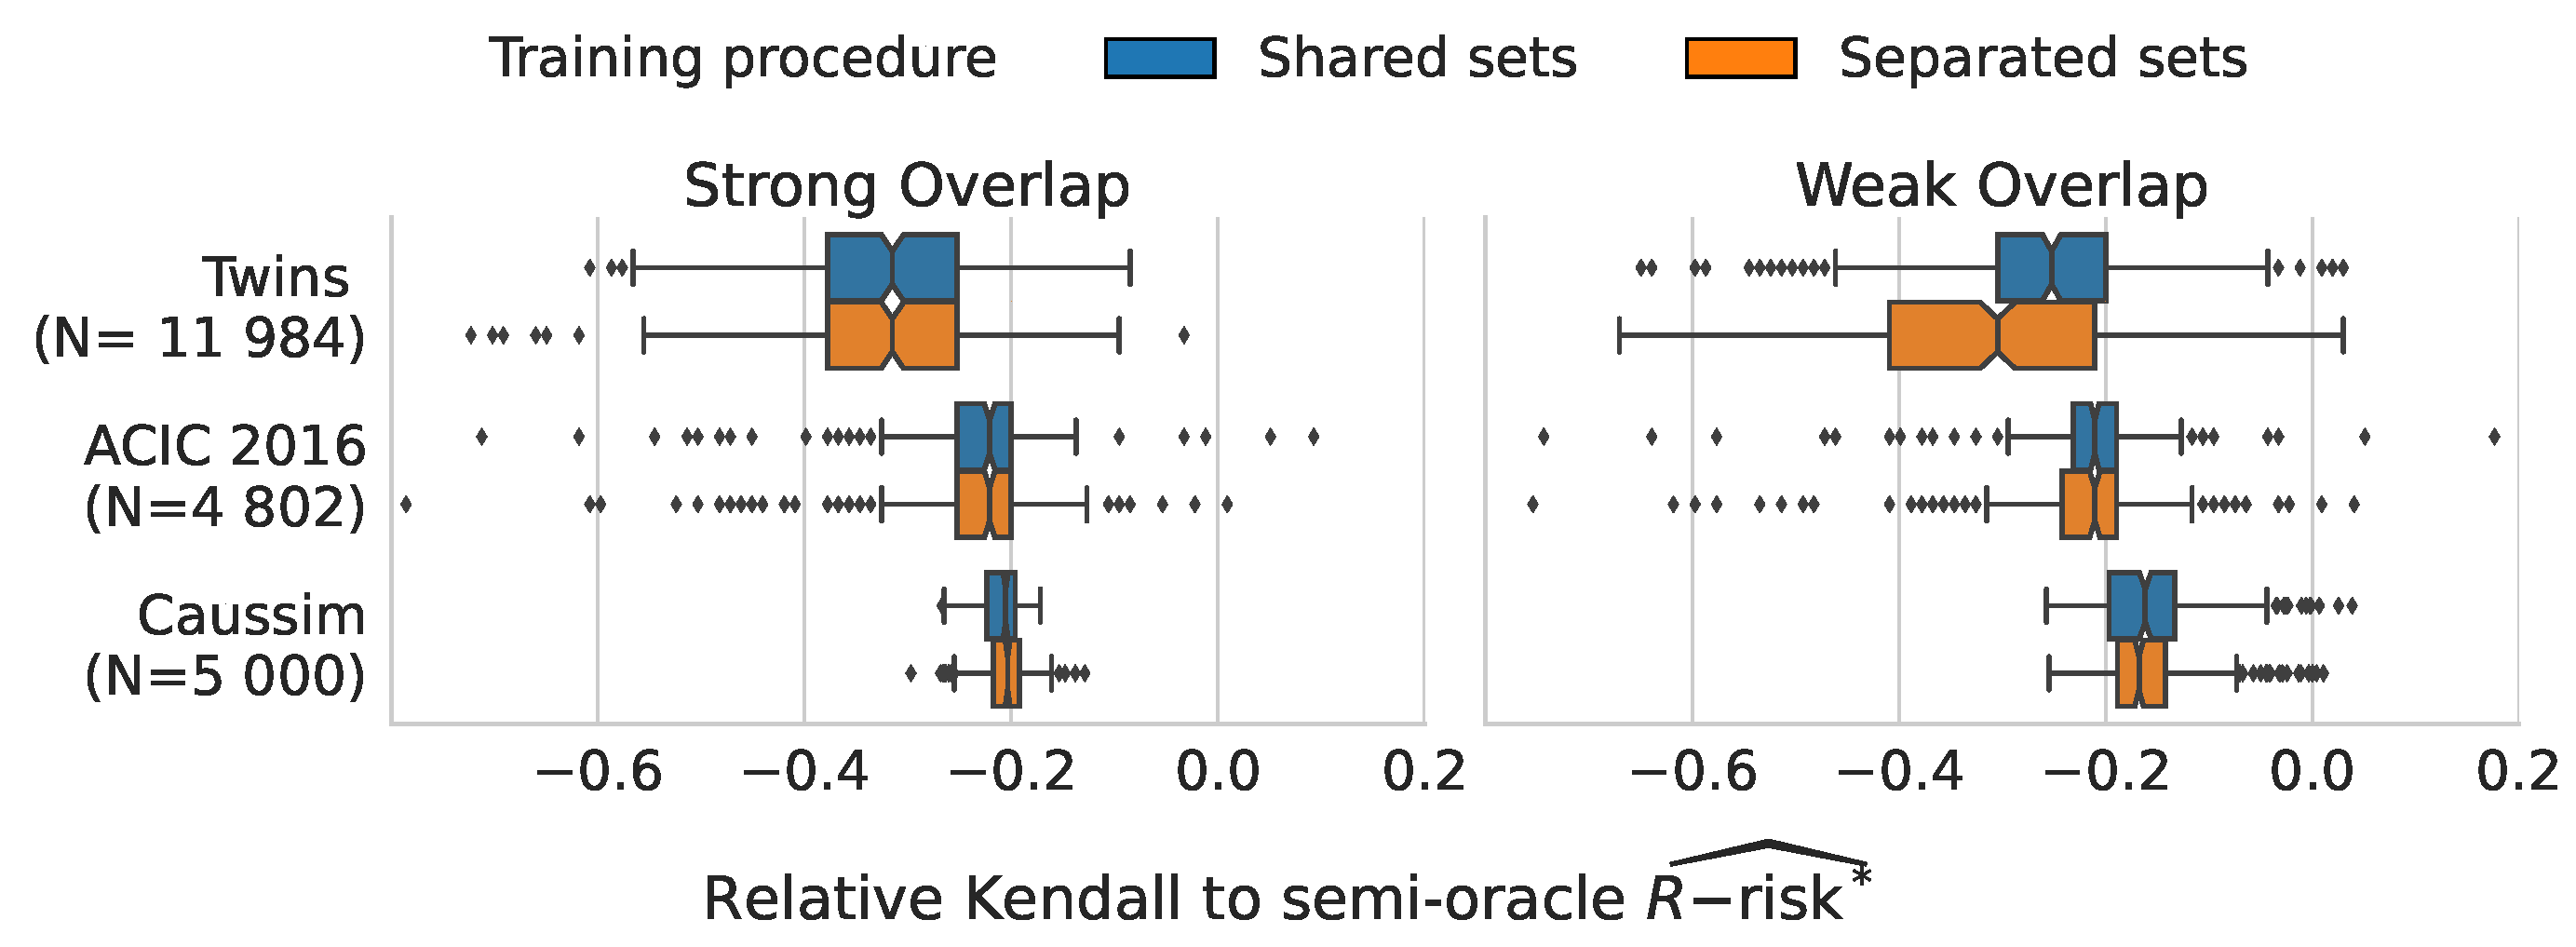
\includegraphics[width=\linewidth]{img/chapter_5/_3_procedure_r_risk_only_3datasets.pdf}
  \caption{\textbf{Nuisances can be estimated on the same data as outcome
      models}: Results for the R-risk are similar between the
    \textcolor{MidnightBlue}{shared
      nuisances/candidate set} and
    the \textcolor{RedOrange}{separated nuisances set} procedures. Figure
    \ref{apd:fig:procedures_comparison_all_metrics} details results for all metrics.}\label{fig:procedures_comparison}
\end{figure}


\paragraph{Stacked models are good overall estimators of nuisances}

For every risk, the oracle version recovers better the best estimator.
However,
stacked nuisances estimators (boosting and linear) lead to feasible
metrics with close performances to the oracles ones: the
corresponding estimators recover well-enough the true nuisances.
One may wonder if simpler models for the nuisance could be useful,
in particular in data-poor settings or when the true models are linear.
Figure \ref{fig:all_datasets_nuisances_comparison} compares causal model
selection estimating nuisances with stacked estimators or linear model.
It comprises the Twins data, where the true propensity model is linear,
and a downsampled version of this data, to study a situation favorable to
linear models. In these settings,
stacked and linear estimations of the nuisances performs equivalently.
Detailed analysis (Figure \ref{apd:fig:nuisances_comparison_twins})
confirms that using adaptive models --as built by
stacking linear models and gradient-boosted trees-- suffices to estimate nuisance.

\begin{figure}[!tb]
  \centering
  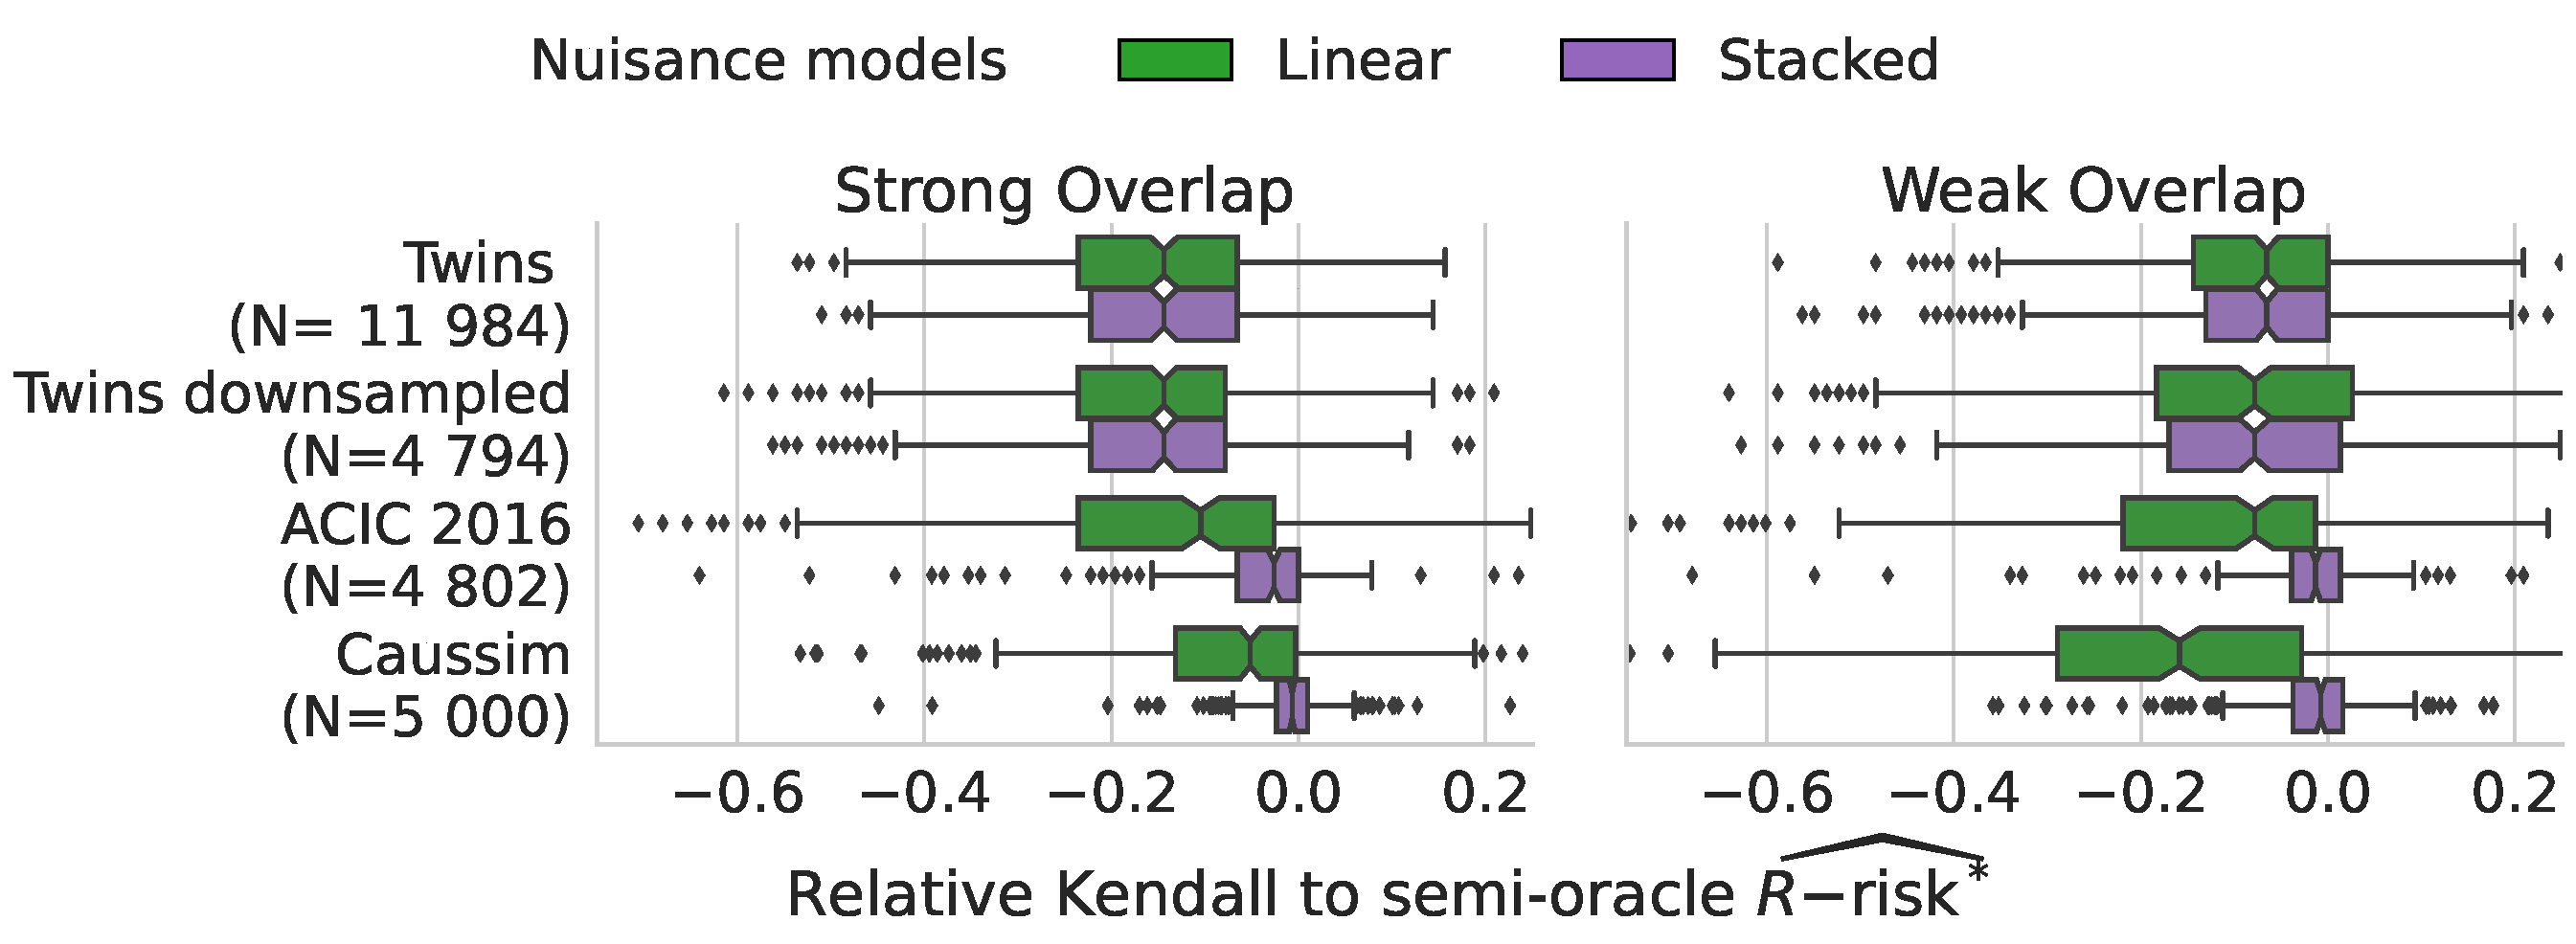
\includegraphics[width=\linewidth]{img/chapter_5/_4_nuisance_models_r_risk_only_3datasets.pdf}
  \caption{\textbf{\textcolor{DarkOrchid}{Stacked
        models} are good overall estimators of the nuisances}:
    Results are shown only for the
    R-risk; Figure \ref{apd:fig:nuisances_comparison}
    details every metrics. For Twins, where the true propensity
    model is linear, \textcolor{DarkOrchid}{stacked} and
    \textcolor{ForestGreen}{linear}
    estimations of the nuisances performs equivalently, even for a downsampled version
    (N=4794). }\label{fig:all_datasets_nuisances_comparison}
\end{figure}

\paragraph{Use 90\% of the data to estimate outcome models, 10\% to
  select them}

The analyst faces a compromise: given a finite
data sample, should she allocate more data to estimate the outcome model,
thus improving the quality of the outcome model but leaving
little data for model selection. Or, she could choose a bigger test set for
model selection and effect estimation. For causal model selection, there
is no established practice (as reviewed in \ref{apd:results:k_fold_choices}).

We investigate such tradeoff varying the ratio between train and test
data size. For this, we first split out 30\% of the data as a holdout set
$\mathcal{V}$ on which we use the oracle response functions to derive
silver-standard estimates of causal quantities. We then
use the standard estimation procedure on the remaining 70\% of the data,
splitting it into train $\mathcal{T}$ and test $\mathcal{S}$ of varying
sizes. We finally measure the error between this estimate and the
silver standard.

We consider two different analytic goals: estimating a average
treatment effect --a single number used for policy making-- and a
CATE --a full model of the treatment effect as a function of covariates
$X$. Given that the latter is a much more complex object than the former,
the optimal train/test ratio might vary. To measure errors, we use for
the ATE the relative absolute ATE bias between the ATE computed with the
selected outcome model on the test set, and the true ATE as evaluated on
the holdout set $\mathcal{V}$. For the CATE, we compare the
$\tau\text{-risk}$
of the best selected model applied on the holdout set $\mathcal{V}$. We explore this trade-off for the ACIC 2016 dataset and the R-risk.

\begin{figure}[!t]
  \begin{minipage}{.5\textwidth}
    \centerline{\textbf{a) CATE estimation error}}
    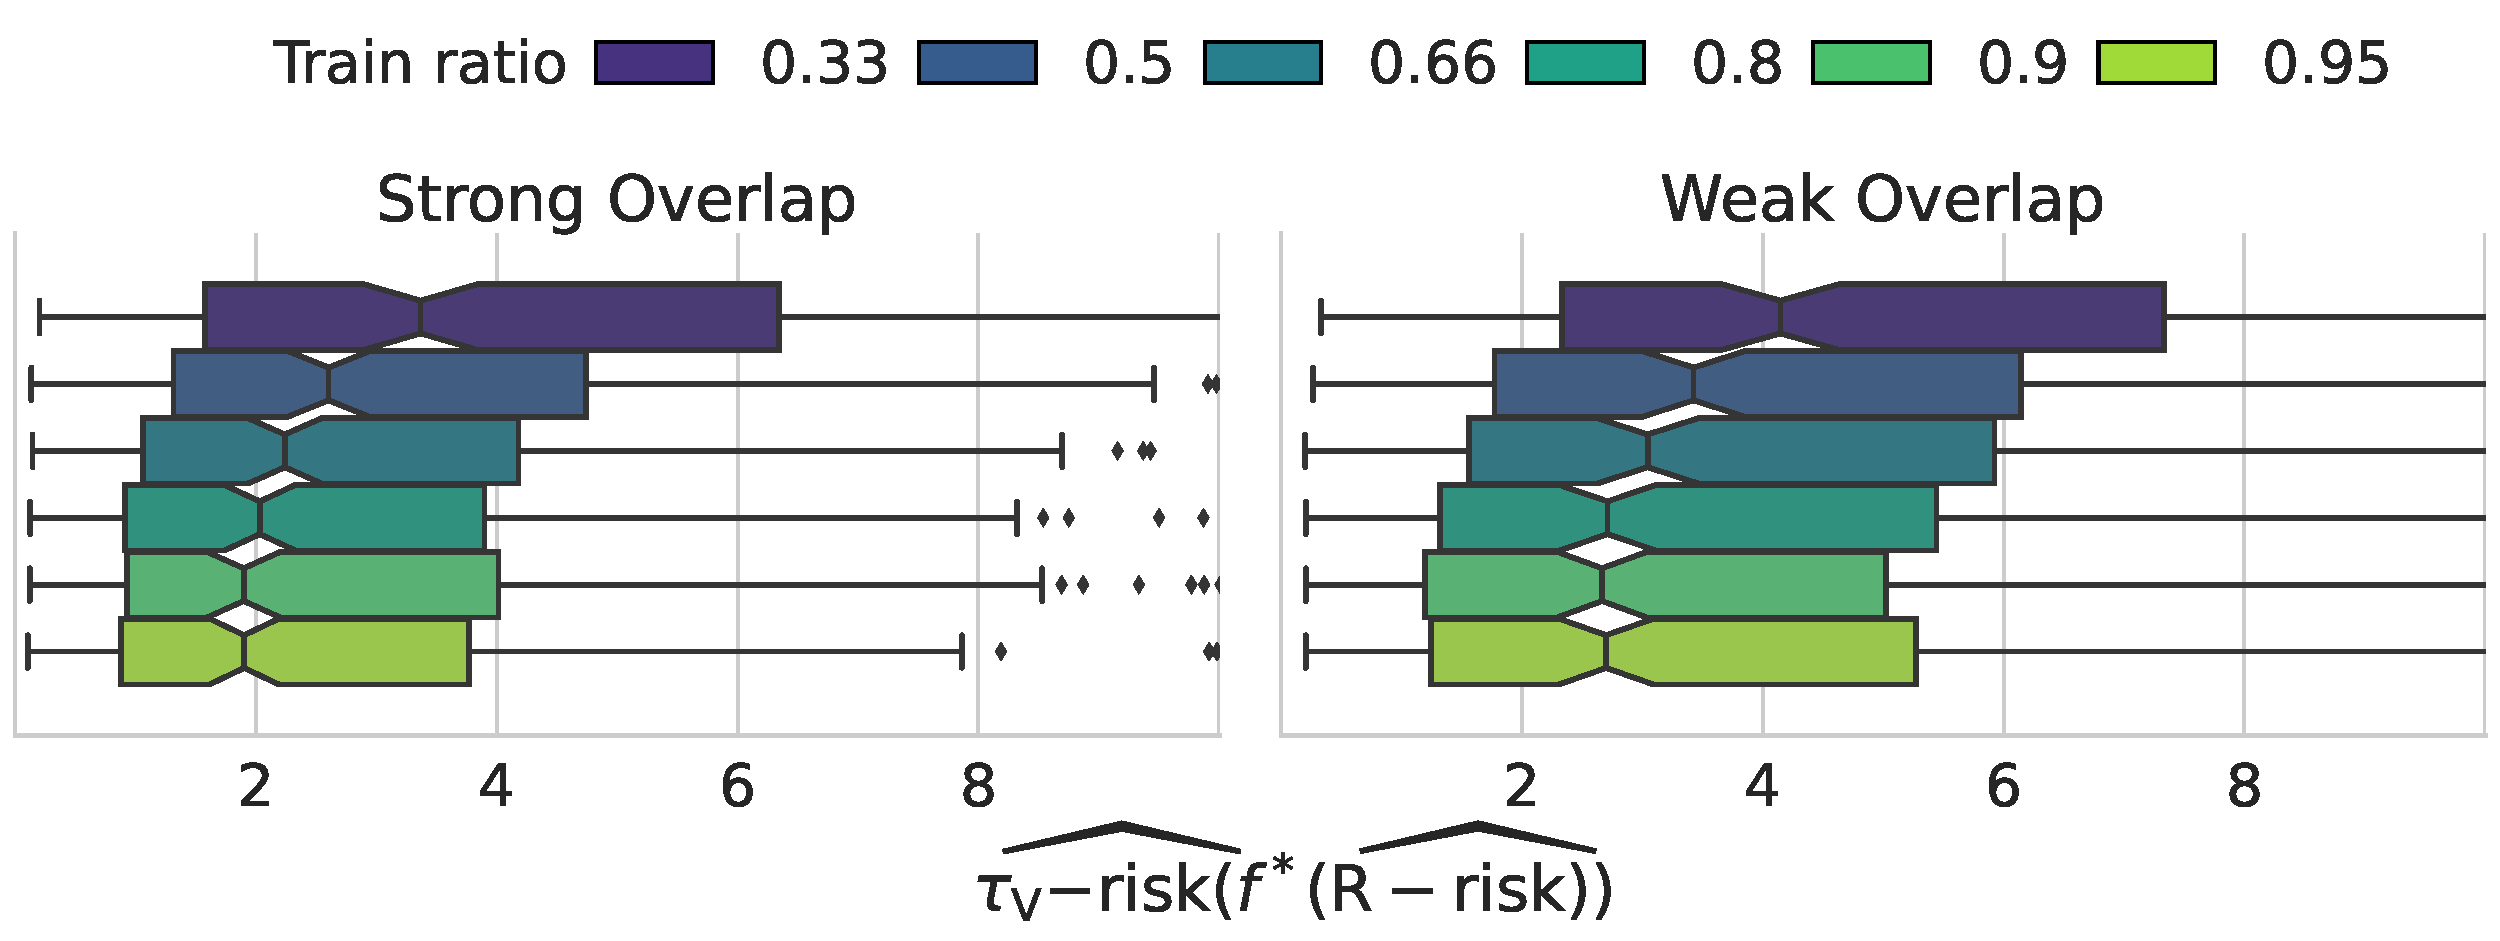
\includegraphics[width=\linewidth]{img/chapter_5/_5_train_size_evaluated_metric_r_risk__evaluation_validation_tau_risk__best_tau_norm__False_norm_False__acic16.pdf}
  \end{minipage}
  %\hspace{0.3\textwidth}
  \begin{minipage}{.5\textwidth}
    \centerline{\textbf{b) ATE estimation error}}
    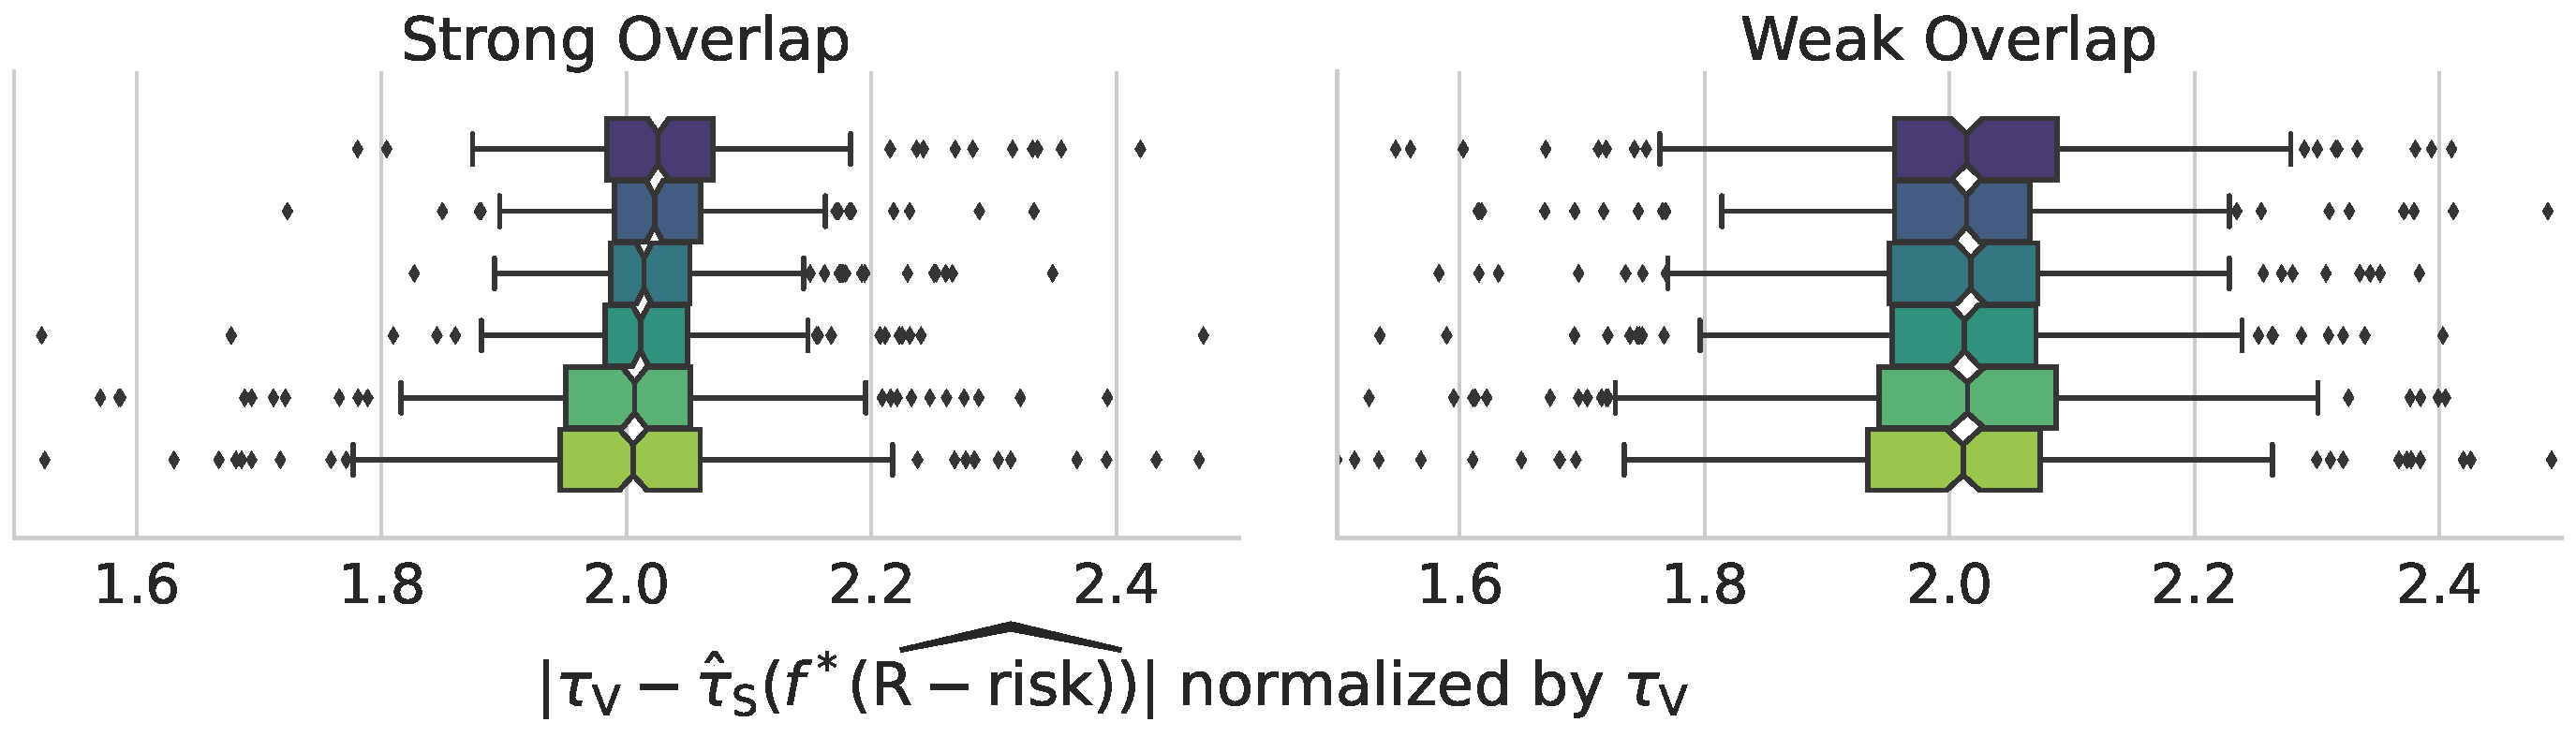
\includegraphics[width=\linewidth]{img/chapter_5/_5_train_size_evaluated_metric_r_risk__evaluation_validation_test_abs_bias_ate__best_tau_norm__False_norm_True__acic16.pdf}
  \end{minipage}%
  \caption{\textbf{a) For CATE, a train/test ratio of 0.9/0.1 appears a good
      trade-off.} b) For ATE, there is a small signal pointing also to
    0.9/0.1 (K=10).
    for ATE. Experiences on 10 replications of all 78 instances of the ACIC 2016
    data.}\label{fig:train_test_ratio}
\end{figure}

Figure \ref{fig:train_test_ratio} shows that a train/test ratio of
0.9/0.1 (K=10) or 0.8/0.2 (K=5) appears best to estimate CATE and
ATE.


\section{Discussion and conclusion}\label{sec:discussion}

Predictive models are increasingly used to reason about causal effects,
for instance in precision medicine to drive individualized decision.
Our results highlight that they should be selected, validated, and tuned
using different procedures and error measures than those classically used
to assess prediction (estimating the so-called $\mu\text{-risk}$).
Rather, selecting the best outcome model according to the $R\text{-risk}$
(eq.\,\ref{def:r_risk}) leads to more valid causal estimates.

\paragraph{Nuisance models: more gain than pain}
%
Estimating the $R\text{-risk}$ requires a more complex procedure than
standard cross-validation used \emph{e.g.}~in machine learning: it involves
fitting nuisance models necessary for model evaluation, though our
results show that these can be learned on the same set of data
as the outcome model evaluated.

The nuisance models must be well estimated (Figure
\ref{fig:all_datasets_nuisances_comparison}). However these models are
easier to select and control than a causally-valid outcome model,
as they are associated to errors on
observed distributions. Our results show that using for nuisance models
a flexible stacking-based family of estimator suffices for good model selection.
%
In fact, a feasible $R\text{-risk}$ --where the nuisances
are estimated-- performs almost as well as an oracle $R\text{-risk}$ --where the
nuisances are known. This may be explained by
results that suggest that estimation errors on both
nuisances partly compensate out in the
$R\text{-risk}$ \citep{daniel2018double,kennedy2020optimal,nie_quasioracle_2017,chernozhukov_double_2018,zivich2021machine,naimi2021challenges}.

Note that propensity score models must be selected to estimate
the individual posterior probability. For this, we used the Brier score,
which is minimized by the true individual probability. An easy mistake is to
use calibration errors popular in machine learning
\citep{platt_probabilistic_1999,zadrozny_obtaining_2001,niculescu-mizil_predicting_2005,minderer_revisiting_2021}
as these select not for the individual posterior probability but for an
aggregate error rate \citep{perez2022beyond}.


\paragraph{Extension to binary outcomes}
While we focused on continuous outcomes, in medicine, the target outcome is
often a categorical variable such as mortality status or diagnosis. In this
case, it may be interesting to focus on other estimands than the Average
Treatment Effect $\mathbb{E}[Y(1)] -\mathbb{E}[Y(0)] $, for instance the
relative risk $\frac{\mathbb P(Y(1) = 1)}{\mathbb P(Y(0) = 1)}$ or the odd
ratio, $\frac{\mathbb P(Y(1) = 1) / [1 - \mathbb P(Y(1) =1)]}{\mathbb P(Y(0) =
  1) / [1 - \mathbb P(Y(0) = 1]}$ are often used \citep{austin2017estimating}.
While the odds ratio is natural for case-control studies \citep{rothman2008case},
other measures can reduce heterogeneity \citep{colnet2023risk}. In the log
domain, the ratios are written as a difference, the framework studied here
(\autoref{sec:causal_model_selection:setting}) can directly apply. In
particular, the log odds ratio is estimated by the common cross-entropy loss (or
log loss) as in logistic regression.

\paragraph{More $R\text{-risk}$ to select models driving decisions}

Prediction models have flourished because their predictions can be easily
demonstrated and validated on left-out data. But they require more
careful validation for decision making, using a metric accounting for the
putative intervention, the $R\text{-risk}$. Even when treated and
untreated population differ little, as in RCTs, the $R\text{-risk}$
brings a sizeable benefit. To facilitate better model selection, we provide Python
code \footnote{\url{https://github.com/soda-inria/causal_model_selection}}.
Using the $R\text{-risk}$ does make evaluation more
complicated not only because the procedure is more involved, but also
because each intervention requires a dedicated evaluation. However, such
off-policy evaluation remains much less costly than the recommended good
practice of impact evaluation testing the ability of a prediction model
to actually guide patient health \citep{hendriksen2013diagnostic}. Also,
the model-selection procedure puts no constraints on the models used to
build predictive models: it opens the door to evaluating a wide range of
models, from gradient boosting to convolutional neutral, or language
models.

%Nevertheless, from a practical perspective, our study establishes that
%the $R\text{-risk}$ is the best option to select predictive models for
%causal inference, without requiring assumptions on the data-generating
%mechanism, the amount of data at hand, or the specific estimators .


% XXX: need a final positive
% Maybe that as our work has no
% requirement on the learning procedure,
% it contributes to ensuring the
% validity of causal inference on complex databases such as clinical
% records with a lot of open-ended text that must be analyzed with
% language models.




\chapter{Conclusion}\label{chapter:conclusion}

%Healthcare burden in modern world is access to healthcare, and chronic disease
%ie. resource issues more than better products, our methodological toolbox to
%distinguish between good and bad management is not adapted to the task since it
%involved complicated process specific to each situation. Some can be borrowed
%from economics, but specificities from epidemiology should be mixed in. 
Modern healthcare burdens and costs are driven by chronic diseases where death
is not the only outcome of interest. Focus on smaller rewards, on which
experiments are easier to conduct and where error is possible: it would allow
better learning for decision making since we can repeat more experiments (limit:
signals could be highly delayed).

Modern collection of data in healthcare makes it a domain closer to social
sciences than usually considered. It involves institutions and individuals with
complex data collection patterns and choices that are seldom well controlled by
the researcher alone: \textit{l'espace général du savoir n'est plus celui des
identités et des différences, [...]celui d'une caractérisation universelle,
d'une taxinomia générale [...], mais un espace fait d'organisations,
c'est-à-dire de rapports internes entre des éléments dont l'ensemble assure une
fonction} \citep{foucault1990mots}. Therefore, we should bridge traditional
statistics with econometrics and social sciences to analyze it. This does not
impose to abandon the scientific method, but to adapt it to constant
distribution shifts and unkown complex mechanisms.

% Pattern exists in the massive data collected: we need to extract them
% automatically and articulate these with scientific questions guided by
% knowledge domain.
Complex patterns in big data call for machine learning methods, which haveq been shown to
highly perform . Text is pervasive, we are using it to communicate and to log
most of our information. We can rely pretraining models outside the healthcare
domain. We should leverage it more in the context of care (limit: temporality is
hard to capture but is a key aspect of causal inference).

% Those problem are more pragmatic than theoretical. Thus, data and conclusions need to circulate. 
The unreasonable effectiveness of healthcare data is yet out of reach due to
hugely difficult transfer of models or administrative barriers to access data
(due to multiplicity of the involved actors). This forces us to rely on
efficient techniques that make the best of medium-sized data or rely on sharable
sources of knowledge (aggregated statistics, federated learning approaches,
ontologies, ...).

\clearpage
%sloppy
%\bibliographystyle{hdr_abbrvnat}
%\bibliographystyle{abbrvnat}
%\bibliographystyle{plainnat}
\begin{multicols}{2}
  \printbibliography
\end{multicols}

\clearpage
\begin{appendices}

  %\addappheadtotoc
  %\section{Statistical models}\label{apd:statistical_models}

  %\section{Causal Diagrams}\label{apd:causal_diagrams}
  \chapter{Chapter 2}\label{apd:cdw}


  \section*{Supplementary information}
  %\renewcommand{\thesubsection}{\thesection.\alph{subsection}}
  % Include only the SI item label in the paragraph heading. Use the
  % \nameref{label} command to cite SI items in the text.
  \section{List of interviewed stakeholders with their
    teams}\label{apd:cdw:table:expert_teams}

  \begin{table}[!ht]
    \centering
    \begin{tabular}{ll}
      \thickhline
      Clinical Data Warehouse & Teams                                             \\
      \thickhline
      CDW\_AMIENS             & IT : 1,MID : 1                                    \\
      CDW\_ANGERS             & Data Direction : 1                                \\
      CDW\_APHM               & Clinician : 1,CDW team : 2                        \\
      CDW\_APHP               & CDW team : 4,IT : 5                               \\
      CDW\_BORDEAUX           & CDW team : 1,Inserm : 1,public health : 2         \\
      CDW\_BREST              & CDW team : 1,MID : 1                              \\
      CDW\_DIJON              & CDW team : 1                                      \\
      CDW\_EDSAN              & CDW team : 2,MID : 1                              \\
      CDW\_HCL                & Clinician : 1,Data Direction : 1,IT : 1,Inserm    \\
      CDW\_INCLUDE\_LILLE     & Administration : 2,CDW team : 3,public health : 2 \\
      CDW\_MARTINIQUE         & CDW team : 1,public health : 1                    \\
      CDW\_MONTPELLIER        & Data Direction : 2,MID : 1,public health : 1      \\
      CDW\_NANCY              & CDW team : 2,public health : 2                    \\
      CDW\_NANTES             & CDW team : 2,public health : 1                    \\
      CDW\_POITIERS           & IT : 2,CRD : 1                                    \\
      CDW\_PREDIMED\_CHUGA    & CDW team : 3,public health : 2                    \\
      CDW\_REIMS              & Clinician : 1,CDW team : 1                        \\
      CDW\_RENNES             & CDW team : 2,public health : 2                    \\
      CDW\_STRASBOURG         & CDW team : 2,public health : 2                    \\
      CDW\_TOULOUSE           & CDW team : 1                                      \\
      CDW\_TOURS              & CDW team : 1                                      \\
      \thickhline
    \end{tabular}
  \end{table}

  \clearpage


  \begin{landscape}
    \section{Interview form} \label{apd:cdw:interview_form}
    \begin{table}[h!]
      \centering
      \resizebox{1.6\textwidth}{!}{%
        \begin{tabular}{|l|l|}
          \hline
          \textbf{Topics}                                                        &
          \textbf{Questions}
          \\ \hline
          \multirow{5}{*}{\begin{tabular}[c]{@{}l@{}}Initiation and Construction
                              of \\ the Clinical Data Warehouse\end{tabular}} &
          How was the initiative born, when, which team(s) involved in the
          construction? A Data warehouse to meet what initial needs ?                                                                 \\
          \cline{2-2}                                                            & What was (is) the articulation between the medical
          informatics / engineer(s) / Clinical Research Department  and user
          team(s), biostatistics ?                                                                                                    \\ \cline{2-2} & Governance: How
          should the teams be organized for the creation and maintenance of the
          warehouse, data access, and project teams?                                                                                  \\ \cline{2-2} &
          \begin{tabular}[c]{@{}l@{}}What types of data are present in the
            warehouse
            from the
            following
            non-exhaustive
            list: \\
            Billing
            codes ,
            other
            administrative
            data,
            other
            procedures,
            structured
            procedures
            and
            diagnoses,
            structured
            biology
            measures,
            \\
            structured
            drug
            treatments,
            emergencies,
            resuscitation,
            anesthesia,
            texts
            (letters,
            Clinician
            Reports),
            imaging,
            anatomopathology,
            sequencing.\end{tabular}
          \\
          \cline{2-2}
                                                                                 & What
          are the
          medico-social/social
          data,
          especially
          from
          social
          and
          medico-social
          institutions
          ?
          \\
          \hline
          \multirow{6}{*}{Current status - Ongoing and finished projects}        &
          \begin{tabular}[c]{@{}l@{}}Who are the main users? For what purposes
            (research,
            quality
            improvement,
            management,
            clinical
            usage)?
            \\ Which
            therapeutic
            area(s)?\end{tabular}
          \\
          \cline{2-2}
                                                                                 &
          \begin{tabular}[c]{@{}l@{}}What are the major types of projects from the
            following
            non-exhaustive
            list: \\
            Cohort
            development,
            descriptive
            epidemiology,
            analytical
            (comparative)
            epidemiology
            with/without
            randomization,
            monitoring
            and
            dashboards,
            \\indicators,
            inclusion
            in
            clinical
            trials.\end{tabular}
          \\
          \cline{2-2}
                                                                                 & How
          many
          projects
          are
          completed
          /
          started
          /
          planned?
          \\
          \cline{2-2}
                                                                                 & What
          are the
          tools
          and
          methods
          used for
          these
          projects?
          Cohort
          building
          tool,
          standard
          data
          formats,
          NLPs,
          ...
          \\
          \cline{2-2}
                                                                                 & Is
          there a
          valorization
          strategy
          for the
          Clinical
          Data
          Warehouse?
          \\
          \cline{2-2}
                                                                                 & What
          connections
          with
          external
          sources
          such as
          the
          national
          health
          data
          platform,
          the
          outpatient
          data,
          the
          general
          practitioner
          data,
          the
          research
          cohorts
          ?                                                                                                                           \\
          \hline
          \multirow{3}{*}{Opportunity and obstacles}                             & What
          are the main difficulties encountered during data warehouse projects?
          \\ \cline{2-2} & Are there themes that deserve more encouragement from
          the HAS?
          \\ \cline{2-2} & What skills are needed? Are there any skills or
          technical resources missing?
          \\ \hline
          \multirow{11}{*}{\begin{tabular}[c]{@{}l@{}}Quality criteria for
                               observational research\end{tabular}}       & Coverage: How
          is it monitored? Geographically/by department? Time-wise? By what means?
          \\ \cline{2-2} & Cleaning: How are patient duplicates and source
          alignment managed?
          \\ \cline{2-2} &
          \begin{tabular}[c]{@{}l@{}}Database Network: Does the warehouse belong
            to a
            health
            database
            network?\end{tabular}
          \\
          \cline{2-2}
                                                                                 &
          \begin{tabular}[c]{@{}l@{}}Data quality: Are there automatic reports on
            data
            quality?
            Frequency,
            design,
            code and
            documentation
            available?
            Presence
            of
            dedicated
            personnel
            \\ or
            even a
            team to
            check
            the
            quality
            of the
            data
            continuously,
            and to
            carry
            out
            quality
            controls
            of the
            data on
            the
            central
            base, on
            the
            study
            bases?\end{tabular}
          \\
          \cline{2-2}
                                                                                 &
          \begin{tabular}[c]{@{}l@{}}Data life cycle: Is there a reference
            document
            on the
            different
            stages
            of the
            data
            life
            cycle?
            \\ How
            is this
            document
            kept up
            to date
            with the
            constant
            evolution
            of the
            warehouse?
            In what
            form? \\
            How is
            this
            documentation
            managed,
            accessed,
            updated
            and
            corrected?
            Precise
            description
            of the
            integrated
            fields?\end{tabular}
          \\
          \cline{2-2}
                                                                                 &
          \begin{tabular}[c]{@{}l@{}}Harmonization procedure: What are the data
            structures/formats
            and
            coding
            systems
            used? \\
            (eHop,
            I2B2,
            OMOP,
            HL7
            FHIR,
            other
            ?)\end{tabular}
          \\
          \cline{2-2}
                                                                                 &
          \begin{tabular}[c]{@{}l@{}}Machine learning: If machine learning systems
            are used
            (e.g.
            for
            extracting
            and
            structuring
            information),
            is there
            specific
            documentation
            on their
            performance?
            \\ For
            manual
            coding
            (e.g.
            labelling),
            is there
            a coding
            guide?
            Has a
            measurement
            of
            inter-coder
            consistency
            been
            conducted?\end{tabular}
          \\
          \cline{2-2}
                                                                                 &
          De-identification:
          Elements
          on
          de-identification
          if
          applicable,
          performance
          metrics
          \\
          \cline{2-2}
                                                                                 &
          \begin{tabular}[c]{@{}l@{}}Constructed phenotypes: Are there operational
            definitions
            of
            target
            populations
            (study
            cohorts)
            and how
            are
            these
            compared
            to
            conceptual
            definitions,
            i.e., \\
            business
            and
            scientific
            definitions?
            Is there
            a study
            of
            FPR/TPR
            in
            relation
            to a
            reference
            standard?
            Are
            these
            definitions
            made
            public
            either
            with the
            study \\
            results
            or in
            the
            documentation
            of the
            warehouse?\end{tabular}
          \\
          \cline{2-2}
                                                                                 &
          \begin{tabular}[c]{@{}l@{}}Transparency: Are the studies registered on a
            dedicated
            or
            pre-existing
            portal
            (epidemio-France,
            encepp
            (EU),
            clinicaltrials.gov
            (US))?
            \\ Are
            the
            study
            codes
            made
            accessible
            as for
            opensafely?
            Are the
            publications
            accessible
            in open
            access,
            once the
            studies
            are
            completed?\end{tabular}
          \\
          \cline{2-2}
                                                                                 &
          \begin{tabular}[c]{@{}l@{}}Multidisciplinarity: Are the project teams
            multidisciplinary? Specification of the participations for each part of
            the analysis from the data collection \\ from the raw Information
            System.\end{tabular}
          \\ \hline
          \multirow{2}{*}{Topics of interest to the HAS}                         &
          \begin{tabular}[c]{@{}l@{}}Quality Department: quality indicators
            (french
            IQSS):
            coordination
            (patient
            assessment
            for
            discharge,
            patient
            contact
            at D+1),
            quality
            of the
            liaison
            letter),
            \\
            management
            (eligibility
            for the
            outpatient
            surgeries,
            pain
            management)\end{tabular}
          \\
          \cline{2-2}
                                                                                 &
          \begin{tabular}[c]{@{}l@{}}Health Technology Assessment Department:
            hospital biology activity (description), adverse events associated with
            procedures, post-registration studies \\(procedures, early access
            oncology). Evaluation of procedures: e.g. biological and imaging
            procedures performed in hospitals, genetic tests in oncology and rare
            diseases.\end{tabular}
          \\ \hline
          open discussion                                                        &                                                    \\
          \hline
        \end{tabular}%
      }
      %\caption*{Interview form.}

    \end{table}
  \end{landscape}

  \section{Study data tables}\label{apd:cdw:study_tables}

  The data tables used to produce the figures in the results section are available
  at the following url:

  \url{https://gitlab.has-sante.fr/has-sante/public/rapport_edsh/}.

  The guests table concerns the individuals interviewed, the interview dates, the
  positions and the membership of a specific team. The warehouse table collects
  information about the CDW. The table of studies is the referencing of the
  studies informed on 10 portals of studies in progress (or completed if
  available) available in free access.
  \chapter{Chapter 5}\label{apd:causal_model_selection}


  \section{Variability of ATE estimation on ACIC 2016}%

  \label{apd:toy_example:acic_2016_ate_variability}%

  Figure \ref{fig:acic_2016_ate_heterogeneity} shows ATE estimations for six
  different models used in g-computation estimators on the 76 configurations of
  the ACIC 2016 dataset. Outcome models are fitted on half of the data and
  inference is done on the other half --ie. train/test with a split ratio of 0.5.
  For each configuration, and each model, this train test split was repeated ten
  times, yielding non parametric variance estimates
  \citep{bouthillier_accounting_2021}.

  Outcome models are implemented with
  \href{https://scikit-learn.org/stable/}{scikit-learn}
  \citep{pedregosa_scikitlearn_2011} and the following hyper-parameters:

  \begin{table}[h!]
    \centering
    \resizebox{0.5\linewidth}{!}{%

      \begin{tabular}{llll}
        \toprule
        Outcome Model                                  & Hyper-parameters grid
        \\
        \midrule
        Random Forests                                 & Max depth: [2,
        10]                                                                    \\

        Ridge regression without treatment interaction & Ridge regularization:
        [0.1]                                                                  \\

        Ridge regression with treatment interaction    & Ridge regularization:
        [0.1]                                                                  \\
        \bottomrule
      \end{tabular}
    }
    \caption{Hyper-parameters grid used for ACIC 2016 ATE variability}
    \label{apd:toy_example:acic_2016_ate_variability:table}
  \end{table}


  %  \section{Causal assumptions}\label{background:causal_assumptions}

  \section{Proofs: Links between feasible and oracle risks}\label{apd:proofs}

  \subsection{Upper bound of $\tau\text{-risk}$ with
    $\mu\text{-risk}_{IPW}$}%
  \label{apd:proofs:mu_risk_ipw_bound}%

  For the bound with the $\mu\text{-risk}_{IPW}$, we will decompose the CATE risk
  on each factual population risks:

  \begin{definition}[Population Factual $\mu\text{-risk}$]\label{mu_risk_a}
    \citep{shalit_estimating_2017}
    \begin{equation*}
      \mu\text{-risk}_{a}(f)= \int_{\mathcal Y \times \mathcal X} (y-f(x ; A=a))^{2}  p(y ; x=x \mid A=a) \; dy dx
    \end{equation*}
  \end{definition}

  Applying Bayes rule, we can decompose the $\mu\text{-risk}$ on each
  intervention:
  \begin{equation*}
    \mu\text{-risk}(f)
    =p_{A} \,\mu\text{-risk}_{1}(f)+\left(1-p_{A}\right) \,\mu\text{-risk}_{0}(f)
    \text{with } p_A=\mathbb P(A=1)
  \end{equation*}

  These definitions allows to state a intermediary result on each population:
  \begin{lemma}[Mean-variance decomposition]\label{apd:proofs:mu_risk_ipw_link_mu}
    We need a reweighted version of the classical mean-variance decomposition.

    For an outcome model $f: x \times A \rightarrow \mathcal X$. Let the inverse
    propensity weighting function $w(a ; x)=a e(x)^{-1}+(1-a)(1-e(x))^{-1}$.
    \begin{align*}
       & \int_{\mathcal X}(\mu_{1}(x)-f(x ; 1))^{2} p(x) dx  = p_{A} \mu\text{-risk}_{IPW, 1}(w, f)  -\sigma^{2}_{Bayes}(1)
    \end{align*}
    And
    \begin{align*}
       & \int_{\mathcal X}(\mu_{0}(x)-f(x; 0))^{2} p(x) dx   = (1-p_A) \mu\text{-risk}_{IPW, 0}(w, f)  -\sigma^{2}_{Bayes}(0)
    \end{align*}

    \begin{proof}
      \begin{align*}
         & p_{A} \mu\text{-risk}_{IPW, 1}(w, f)  = \int_{\mathcal X \times \mathcal Y} \frac{1}{e(x)}(y-f(x ; 1))^{2} p(y \mid x ; A=1) p(x ; A=1) d y d x                                                      \\
         & = \int_{\mathcal X \times \mathcal Y} (y-f(x ; 1))^{2} p(y \mid x ; A=1) \frac{p(x ; A=1)}{p(x ; A=1)}p(x)dy dx                                                                                      \\
         & = \int_{\mathcal X \times \mathcal Y} \big[(y-\mu_1(x))^{2}+\left(\mu_{1}(x)-f(x ; 1)\right)^{2} + 2\left(y-\mu_{1}(x)\right)\left(\mu_{1}(x)-f(x, 1)\right) \big] p(y \mid x ; A=1) p(x) d y d x    \\
         & =\int_{\mathcal X} \big [ \int_{\mathcal Y} (y-\mu_1(x))^{2} p(y \mid x ; A=1) dy\big ] p(x)dx + \int_{\mathcal X \times \mathcal Y} \left(\mu_{1}(x)-f(x ; 1)\right)^{2} p(x)p(y \mid x ; A=1)dx dy \\
         & + \qquad 2 \int_{\mathcal X} \big [ \int_{\mathcal Y} \left(y-\mu_{1}(x)\right) p(y \mid x ; A=1) dy \big ] \left(\mu_{1}(x)-f(x, 1)\right)p(x)dx                                                    \\
         & =\int_{\mathcal X} \sigma_{y}^{2}(x, 1) p(x) d x +\int_{\mathcal X} \left(\mu_{1}(x)-f(x ; 1)\right)^{2} p(x) d x+0
      \end{align*}
    \end{proof}
  \end{lemma}

  \begin{proposition*}[Upper bound with mu-IPW]\label{apd:proofs:prop:upper_bound}
    Let f be a given outcome model, let the weighting function $w$ be the Inverse
    Propensity Weight $w(x; a) = \frac{a}{e(x)} + \frac{1-a}{1-e(x)}$. Then, under
    overlap (assumption \ref{assumption:overlap}),
    \begin{align*}
      \tau\text{-risk}(f) \leq & \; 2 \, \mu\text{-risk}_{IPW}(w, f)  \; - 2 \, (\sigma^2_{Bayes}(1) +  \sigma^2_{Bayes}(0))
    \end{align*}

    \begin{proof}
      \begin{align*}
         & \tau\text{-risk}(f) =\int_{\mathcal X}(\mu_{1}(x)-\mu_{0}(x)-(f(x ; 1)-f(x ; 0))^{2} p(x) d x
      \end{align*}
      By the triangle inequality $(u+v)^2 \leq 2(u^2 + v^2)$:
      \begin{multline*}
        \tau\text{-risk}(f) \leq
        2 \int_{\mathcal X}\big[\left(\mu_{1}(x)-f(x ; 1)\right)^{2}+ \\ \left(\mu_{0}(x)-f(x ; 0)\right)^{2}\big] p(x) d x
      \end{multline*}
      Applying Lemma \ref{apd:proofs:mu_risk_ipw_link_mu},
      \begin{align*}
         & \tau\text{-risk}(f) \leq 2\big[p_A \mu\text{-risk}_{IPW, 1}(w, f)  +
         &                                                                                  \\ (1-p_A) \mu\text{-risk}_{IPW, 0}(w, f)(w, f)\big] -2(\sigma^{2}_{Bayes}(0) + \sigma^{2}_{Bayes}(1)) \\
         & = 2 \mu\text{-risk}_{IPW}(w, f)-2(\sigma^{2}_{Bayes}(0) + \sigma^{2}_{Bayes}(1))
      \end{align*}
    \end{proof}
  \end{proposition*}



  \subsection{Reformulation of the $R\text{-risk}$ as reweighted
    $\tau\text{-risk}$}%
  \label{apd:proofs:r_risk_rewrite}%

  \begin{proposition*}[$R\text{-risk}$ as reweighted $\tau
        \text{-risk}$]\label{apd:proofs:prop:r_risk_rewrite}

    \begin{proof}

      We consider the R-decomposition: \citep{robinson_rootnconsistent_1988},
      \begin{equation}\label{apd:eq:r_decomposition}
        y(a) = m(x) + \big( a - e(x) \big) \tau(x) + \varepsilon(x; a)
      \end{equation}
      Where $\mathbb E[\varepsilon(X; A)|X, A] = 0$ We can use it as plug in the
      $R\text{-risk}$ formula:

      \begin{align*}
         & R\text {-risk}(f) =\int_{\mathcal{Y} \times \mathcal{X} \times \mathcal{A}}[(y-m(x))-\big(a-e(x)\big) \tau_f(x)]^{2} p(y ; x ; a) d y d x d a                                     \\
         & =\int_{\mathcal{Y} \times \mathcal{X} \times \mathcal{A}} \left[\big(a-e(x)\big)\tau(x)+\varepsilon(x ; a)-\big(a-e(x)\big) \tau_f(x)\right]^{2} p(y ; x ; a) d y d x da          \\
         & =\int_{\mathcal{X} \times \mathcal{A}}\big(a-e(x)\big)^{2}\big(\tau(x)- \tau_f(x)\big)^{2} p(x ; a) d x d a                                                                       \\
         & + 2  \int_{\mathcal{Y} \times \mathcal{X} \times \mathcal{A}}\big(a-e(x)\big)\big(\tau(x)-\tau_f(x)\big)  \int_{\mathcal{Y}} \varepsilon(x ; a) p(y \mid x ; a) d y p(x ; a)dx da \\
         & +\int_{\mathcal{X} \times \mathcal{A}} \int_{\mathcal{Y}} \varepsilon^{2}(x ; a) p(y \mid x ; a) d y p(x ; a) d x d a
      \end{align*}

      The first term can be decomposed on control and treated populations to force
      $e(x)$ to appear:
      \begin{align*}
         & \int_{\mathcal{X}}\big(\tau(x)-\tau_f(x)\big)^{2}\left[e(x)^{2}p(x;0) + \big(1-e(x)\big)^{2} p(x;1)\right] d x                    \\
         & =\int_{\mathcal{X}}\big(\tau(x)-\tau_f(x)\big)^{2}  \left[e(x)^{2}\big(1-e(x)\big)p(x) + \big(1-e(x)\big)^{2}e(x) p(x)\right] d x \\
         & =\int_{\mathcal{X}}(\tau(x)-\tau_f(x))^{2}(1-e(x)) e(x)[1-e(x)+e(x)] p(x) d x                                                     \\ &=\int_{\mathcal{X}}(\tau(x)-\tau_f(x))^{2}(1-e(x)) e(x) p(x) d x.
      \end{align*}

      The second term is null since, $\mathbb E[\varepsilon(x, a) |X, A]=0$.

      The third term corresponds to the modulated residuals \ref{eq:residuals} :
      $\tilde{\sigma}_B^2(0) + \tilde{\sigma}_B^2(1)$

    \end{proof}
  \end{proposition*}

  \section{Measuring overlap}\label{apd:motivation_ntv}

  \paragraph{Motivation of the Normalized Total Variation}
  %\idea{A simplier measure, NTV seems to capture what we want}
  Computing overlap when working only on samples of the observed distribution,
  outside of simulation, requires a sophisticated estimator of discrepancy
  between distributions, as two data points never have the same exact set of
  features. Maximum Mean Discrepancy \citep{gretton2012kernel} is typically
  used in the context of causal inference
  \citep{shalit_estimating_2017,johansson2022generalization}. However it
  needs a kernel, typically Gaussian, to extrapolate across neighboring
  observations. We prefer avoiding the need to specify such a kernel, as it must
  be adapted to the data which is tricky with categorical or non-Gaussian
  features, a common situation for medical data.

  For simulated and some semi-simulated data, we have access to the probability of
  treatment for each data point, which sample both densities in the same data
  point. Thus, we can directly use distribution discrepancy measures and rely on
  the Normalized Total Variation (NTV) distance to measure the overlap between the
  treated and control propensities. This is the empirical measure of the total
  variation distance \citep{sriperumbudur_integral_2009} between the distributions,
  $TV(\mathbb{P}(X|A=1), \mathbb{P}(X|A=0))$. As we have both distribution sampled
  on the same points, we can rewrite it a sole function of the propensity score, a
  low dimensional score more tractable than the full distribution $\mathbb
    P(X|A)$:

  \begin{equation}\label{eq:ntv}
    \widehat{NTV}(e, 1-e) = \frac{1}{2N} \sum_{i =1}^{N} \big |\frac{e(x_i)}{p_A}-\frac{1-e(x_i)}{1-{p_A}} \big |
  \end{equation}

  Formally, we can rewrite NTV as the Total Variation distance
  between the two population distributions. For a population $O = (Y(A), X, A)
    \sim \mathcal{D}$:

  \begin{align*}
    NTV(O) & = \frac{1}{2N} \sum_{i =1}^{N} \big | \frac{e(x_i)}{p_A}-\frac{1-e(x_i)}{1-{p_A}} \big|         \\
           & = \frac{1}{2N} \sum_{i =1}^{N} \big|\frac{P(A=1|X=x_i)}{p_A}-\frac{P(A=0|X=x_i)}{1-{p_A}} \big|
  \end{align*}

  Thus NTV approximates the following quantity in expectation over the data
  distribution $\mathcal{D}$:

  \begin{align*}
    NTV(\mathcal{D}) & = \int_{\mathcal{X}} \big | \frac{p(A=1|X=x)}{p_A}-\frac{p(A=0|X=x)}{1-{p_A}} \big | p(x)dx \\
                     & = \int_{\mathcal{X}} \big | \frac{p(A=1, X=x)}{p_A}-\frac{p(A=0, X=x)}{1-{p_A}} \big |dx    \\
                     & = \int_{\mathcal{X}} \big | p(X=x|A=1)- p(X=x|A=0) \big |dx
  \end{align*}

  For countable sets, this expression corresponds to the Total Variation distance
  between treated and control populations covariate distributions : $TV(p_0(x),
    p_1(x))$.

  \paragraph{Measuring overlap without the oracle propensity scores:} For ACIC
  2018, or for non-simulated data, the true propensity scores are not known. To
  measure overlap, we rely on flexible estimations of the Normalized Total
  Variation, using gradient boosting trees to approximate the propensity score.
  Empirical arguments for this plug-in approach is given in Figure
  \ref{apd:overlap:ntv_approximation}.

  \paragraph{Empirical arguments}

  We show empirically that NTV is an appropriate measure of overlap by :
  \begin{itemize}
    \item Comparing the NTV distance with the MMD for Caussim which is gaussian
          distributed in Figure \ref{apd:overlap:caussim:mmd_vs_ntv},
    \item Verifying that setups with penalized overlap from ACIC 2016 have a
          higher total variation distance than unpenalized setups in Figure
          \ref{apd:overlap:penalized_overlap}.
    \item Verifying that the Inverse Propensity Weights extrema (the inverse of
          the $\nu$ overlap constant appearing in the overlap Assumption
          \ref{assumption:overlap}) positevely correlates with NTV for Caussim,
          ACIC 2016 and Twins in Figure \ref{apd:ntv_vs_max_ipw}. Even if the same
          value of the maximum IPW could lead to different values of NTV, we
          expect both measures to be correlated : the higher the extrem propensity
          weights, the higher the NTV.
  \end{itemize}


  \paragraph{Estimating NTV in practice}

  Finally, we verify that approximating the NTV distance with a learned plug-in
  estimates of e(x) is reasonnable. We used either a logistic regression or a
  gradient boosting classifier to learn the propensity models for the three
  datasets where we have access to the ground truth propensity scores: Caussim,
  Twins and ACIC 2016. We respectively sampled 1000, 1000 and 770 instances of
  these datasets with different seeds and overlap settings. We first run a
  hyperparameter search with cross-validation on the train set, then select the
  best estimator. We refit on the train set this estimator with or without
  calibration by cross validation and finally estimate the normalized TV with the
  obtained model. This training procedure reflects the one described in Algorithm
  \ref{problem:estimation_procedure:algo} where nuisance models are fitted only on
  the train set.

  The hyper parameters are : learning rate $ \in [1e-3, 1e-2, 1e-1, 1]$, minimum
  samples leaf $\in [2, 10, 50, 100, 200]$ for boosting and L2 regularization $\in
    [1e-3, 1e-2, 1e-1, 1]$ for logistic regression.

  Results in Figure \ref{apd:overlap:ntv_approximation} comparing bias to the true
  normalized Total Variation of each dataset instances versus growing true NTV
  indicate that calibration of the propensity model is crucial to recover a good
  approximation of the NTV.




  \begin{figure}
    \begin{subfigure}[b]{\textwidth}
      \centering
      \caption{\textbf{Uncalibrated classifiers}}
      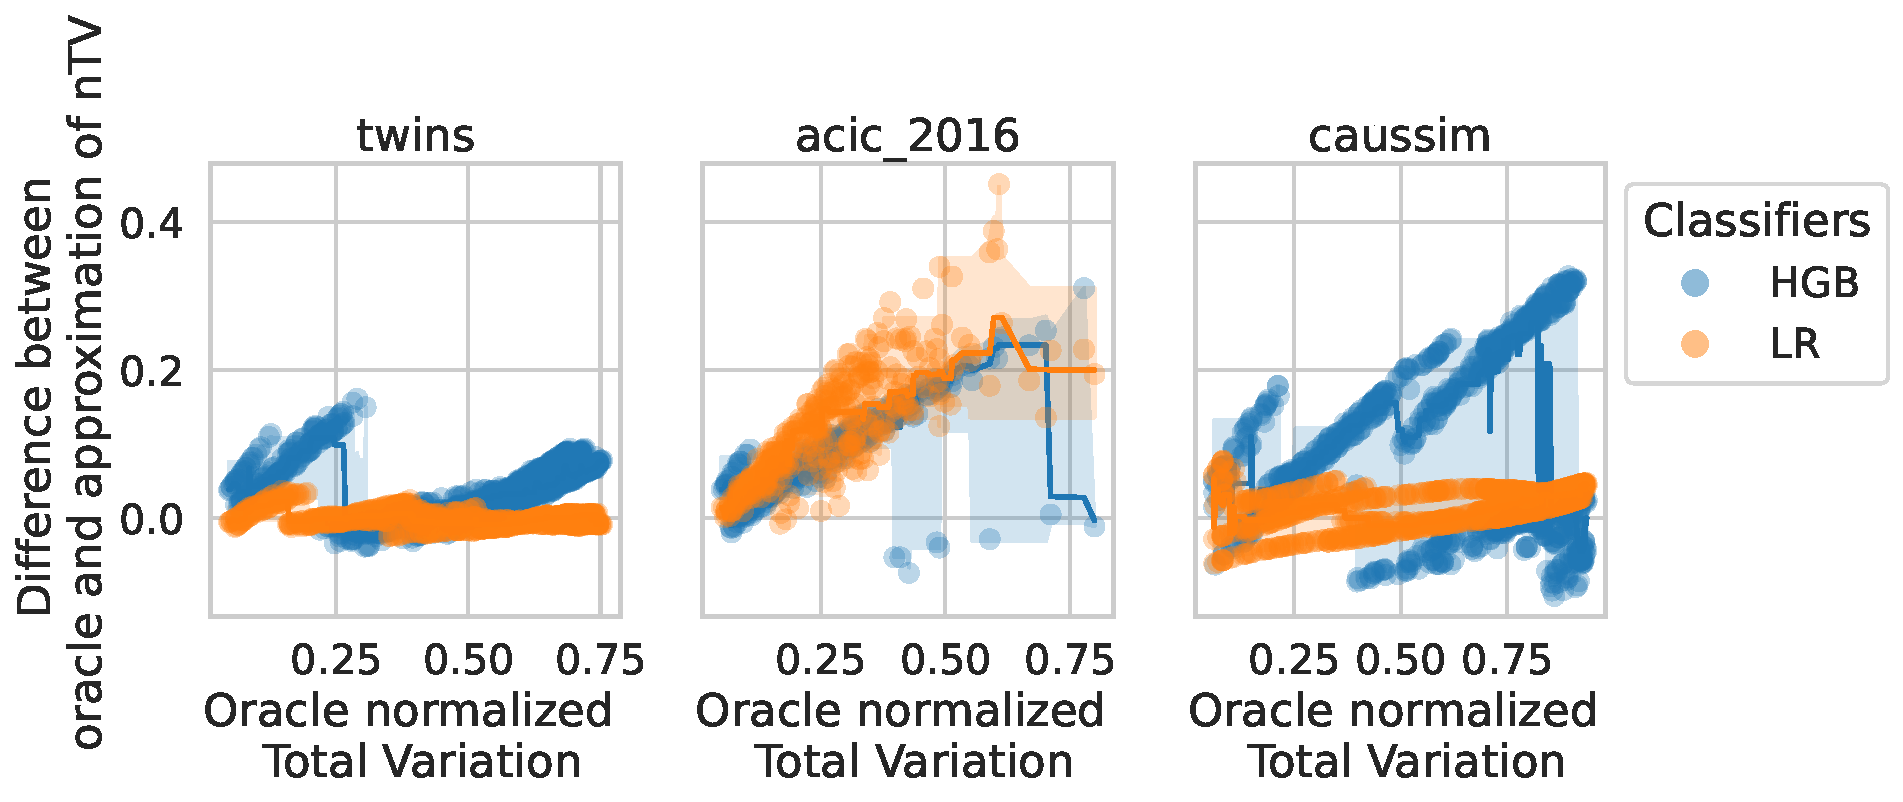
\includegraphics[width=\linewidth]{img/chapter_5/overlap_measure_diff_oracle_ntv_to_n_tv_calibration=False_vs_oracle_n_tv.pdf}
    \end{subfigure}
    \begin{subfigure}[b]{\textwidth}
      \centering
      \caption{\textbf{Calibrated
          classifiers}}
      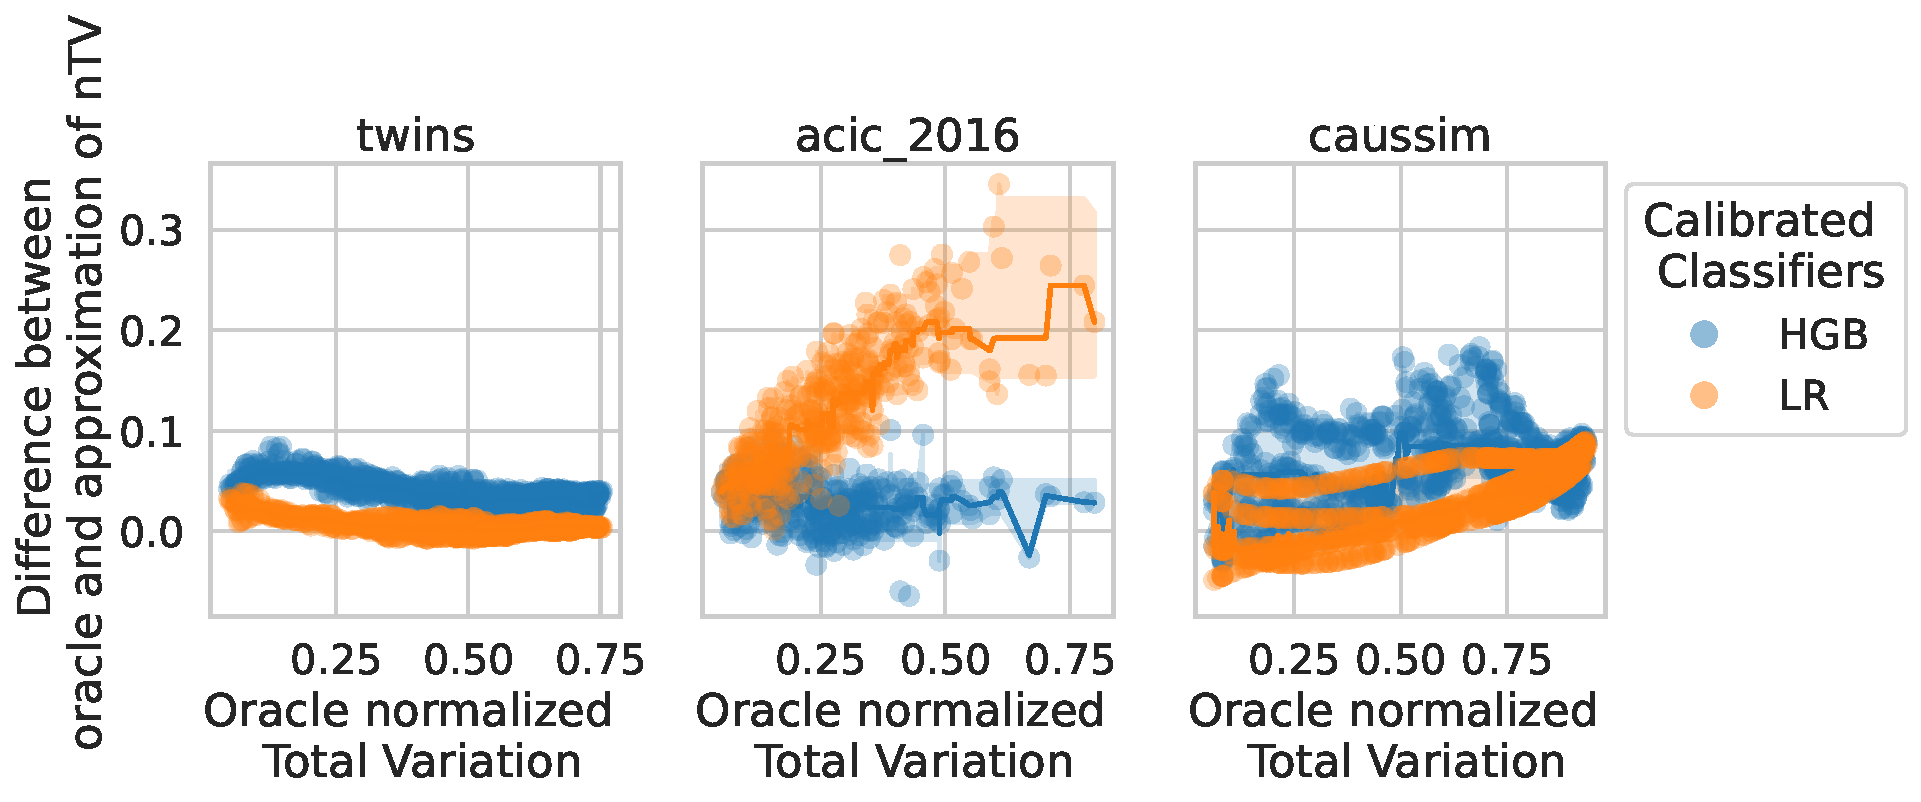
\includegraphics[width=\linewidth]{img/chapter_5/overlap_measure_diff_oracle_ntv_to_n_tv_calibration=True_vs_oracle_n_tv.pdf}
    \end{subfigure}
    \caption{a) Without calibration, estimation of NTV is not trivial even for
      boosting models. b) Calibrated classifiers are able to recover the true
      Normalized Total Variation for all datasets where it is
      available.}\label{apd:overlap:ntv_approximation}
  \end{figure}



  \begin{figure}
    \centering
    \caption{NTV recovers well the overlap settings described in the ACIC paper
      \citep{dorie_automated_2019}}\label{apd:overlap:penalized_overlap}
    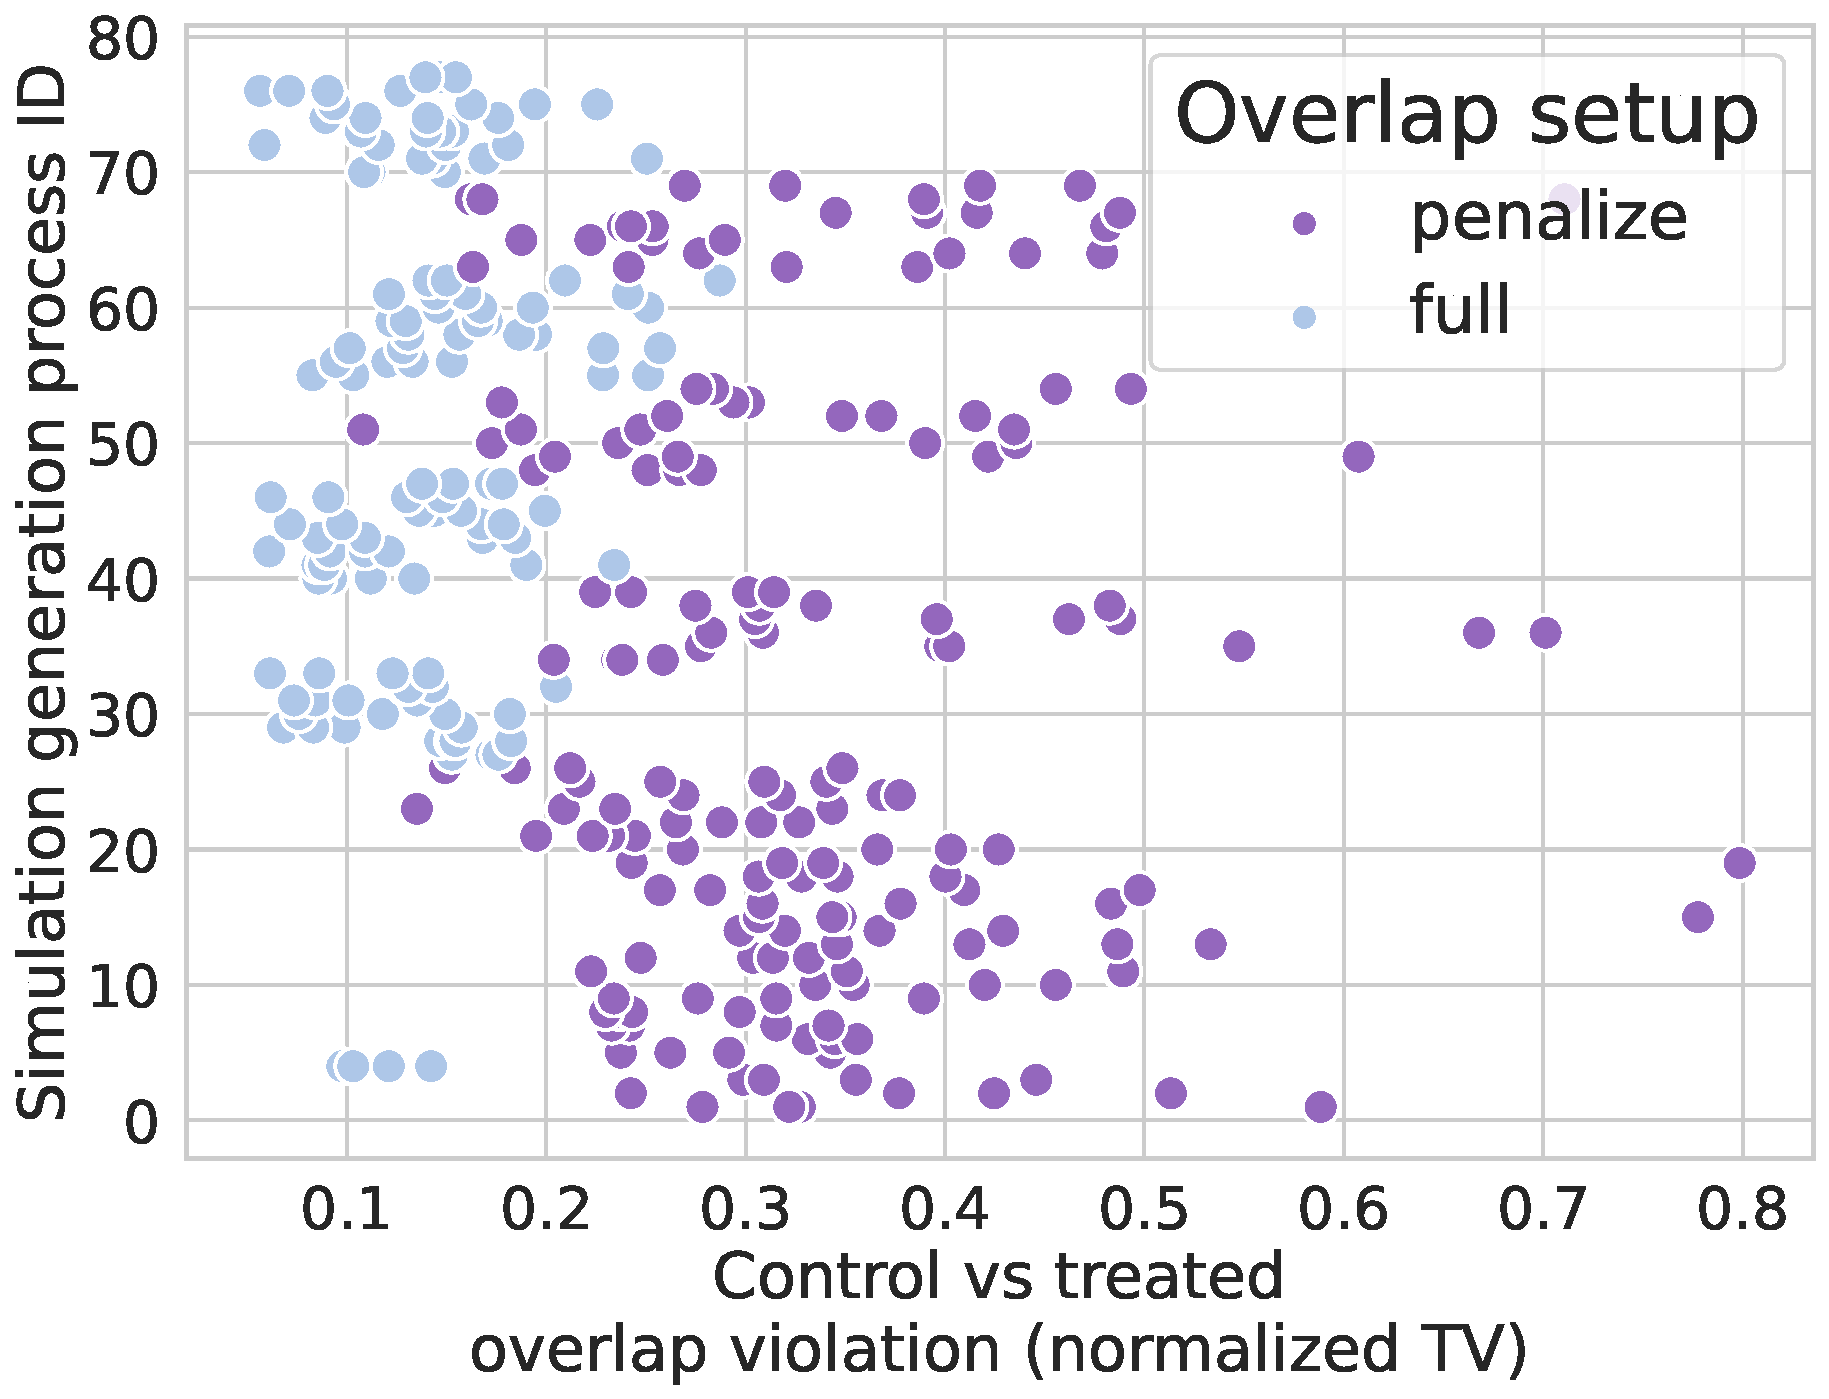
\includegraphics[width=0.7\linewidth]{img/chapter_5/overlap_measure_acic_2016_recovery_overlap_setup.pdf}
  \end{figure}


  \begin{figure}[htbp]
    \centering
    \caption{Good correlation between overlap measured as normalized Total
      Variation and Maximum Mean Discrepancy (200 sampled Caussim
      datasets)}\label{apd:overlap:caussim:mmd_vs_ntv}
    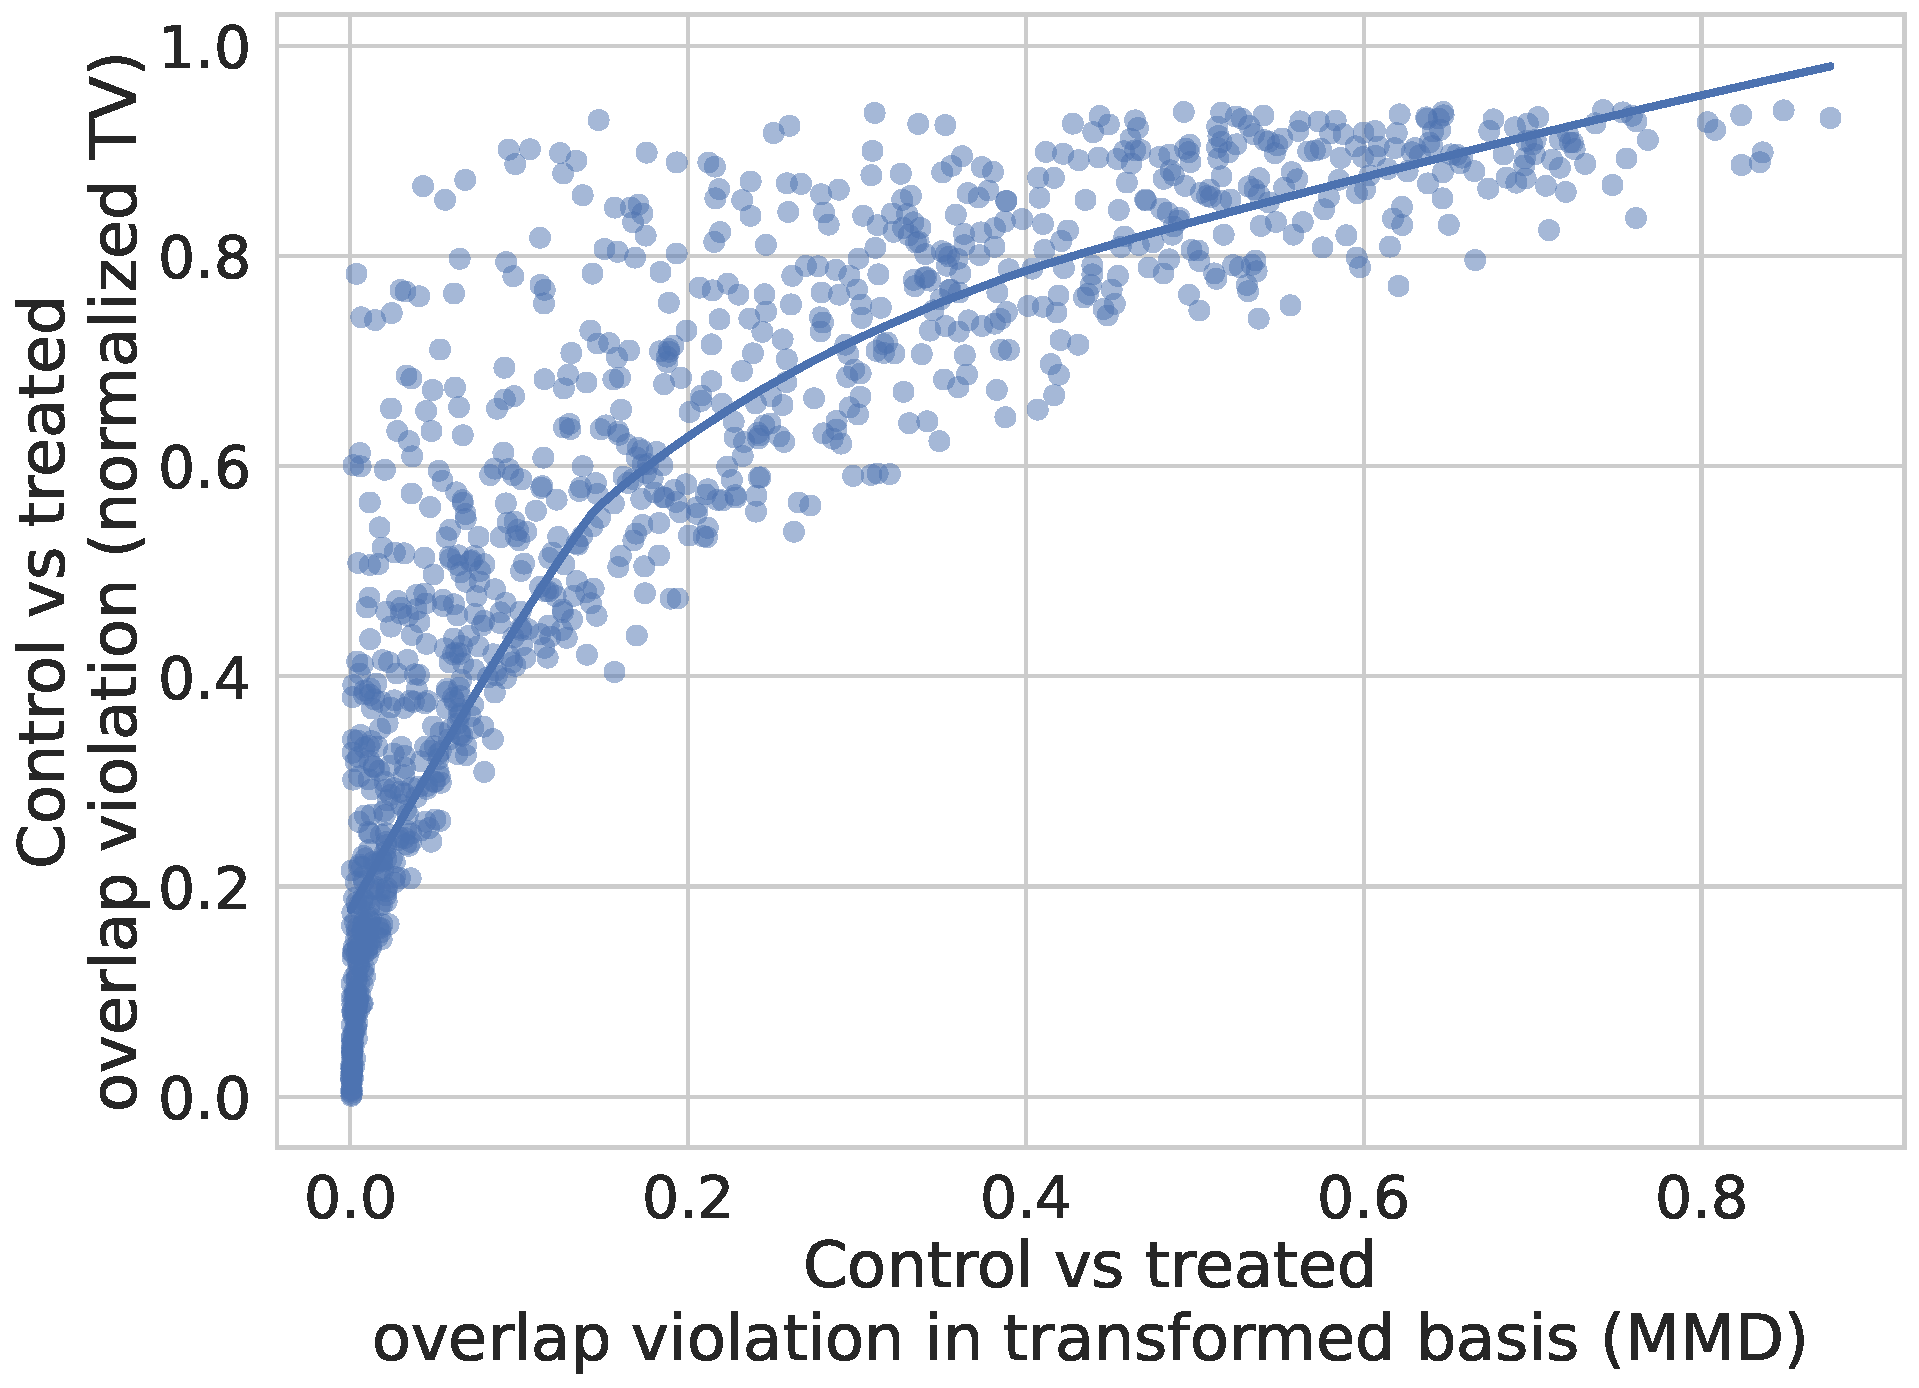
\includegraphics[width=0.7\linewidth]{img/chapter_5/overlap_measure_caussim_transformed_mmd_vs_ntv.pdf}
  \end{figure}


  \begin{figure}[ht]
    \centering
    \begin{subfigure}[b]{0.47\textwidth}
      \centering
      \caption{\textbf{Caussim}}
      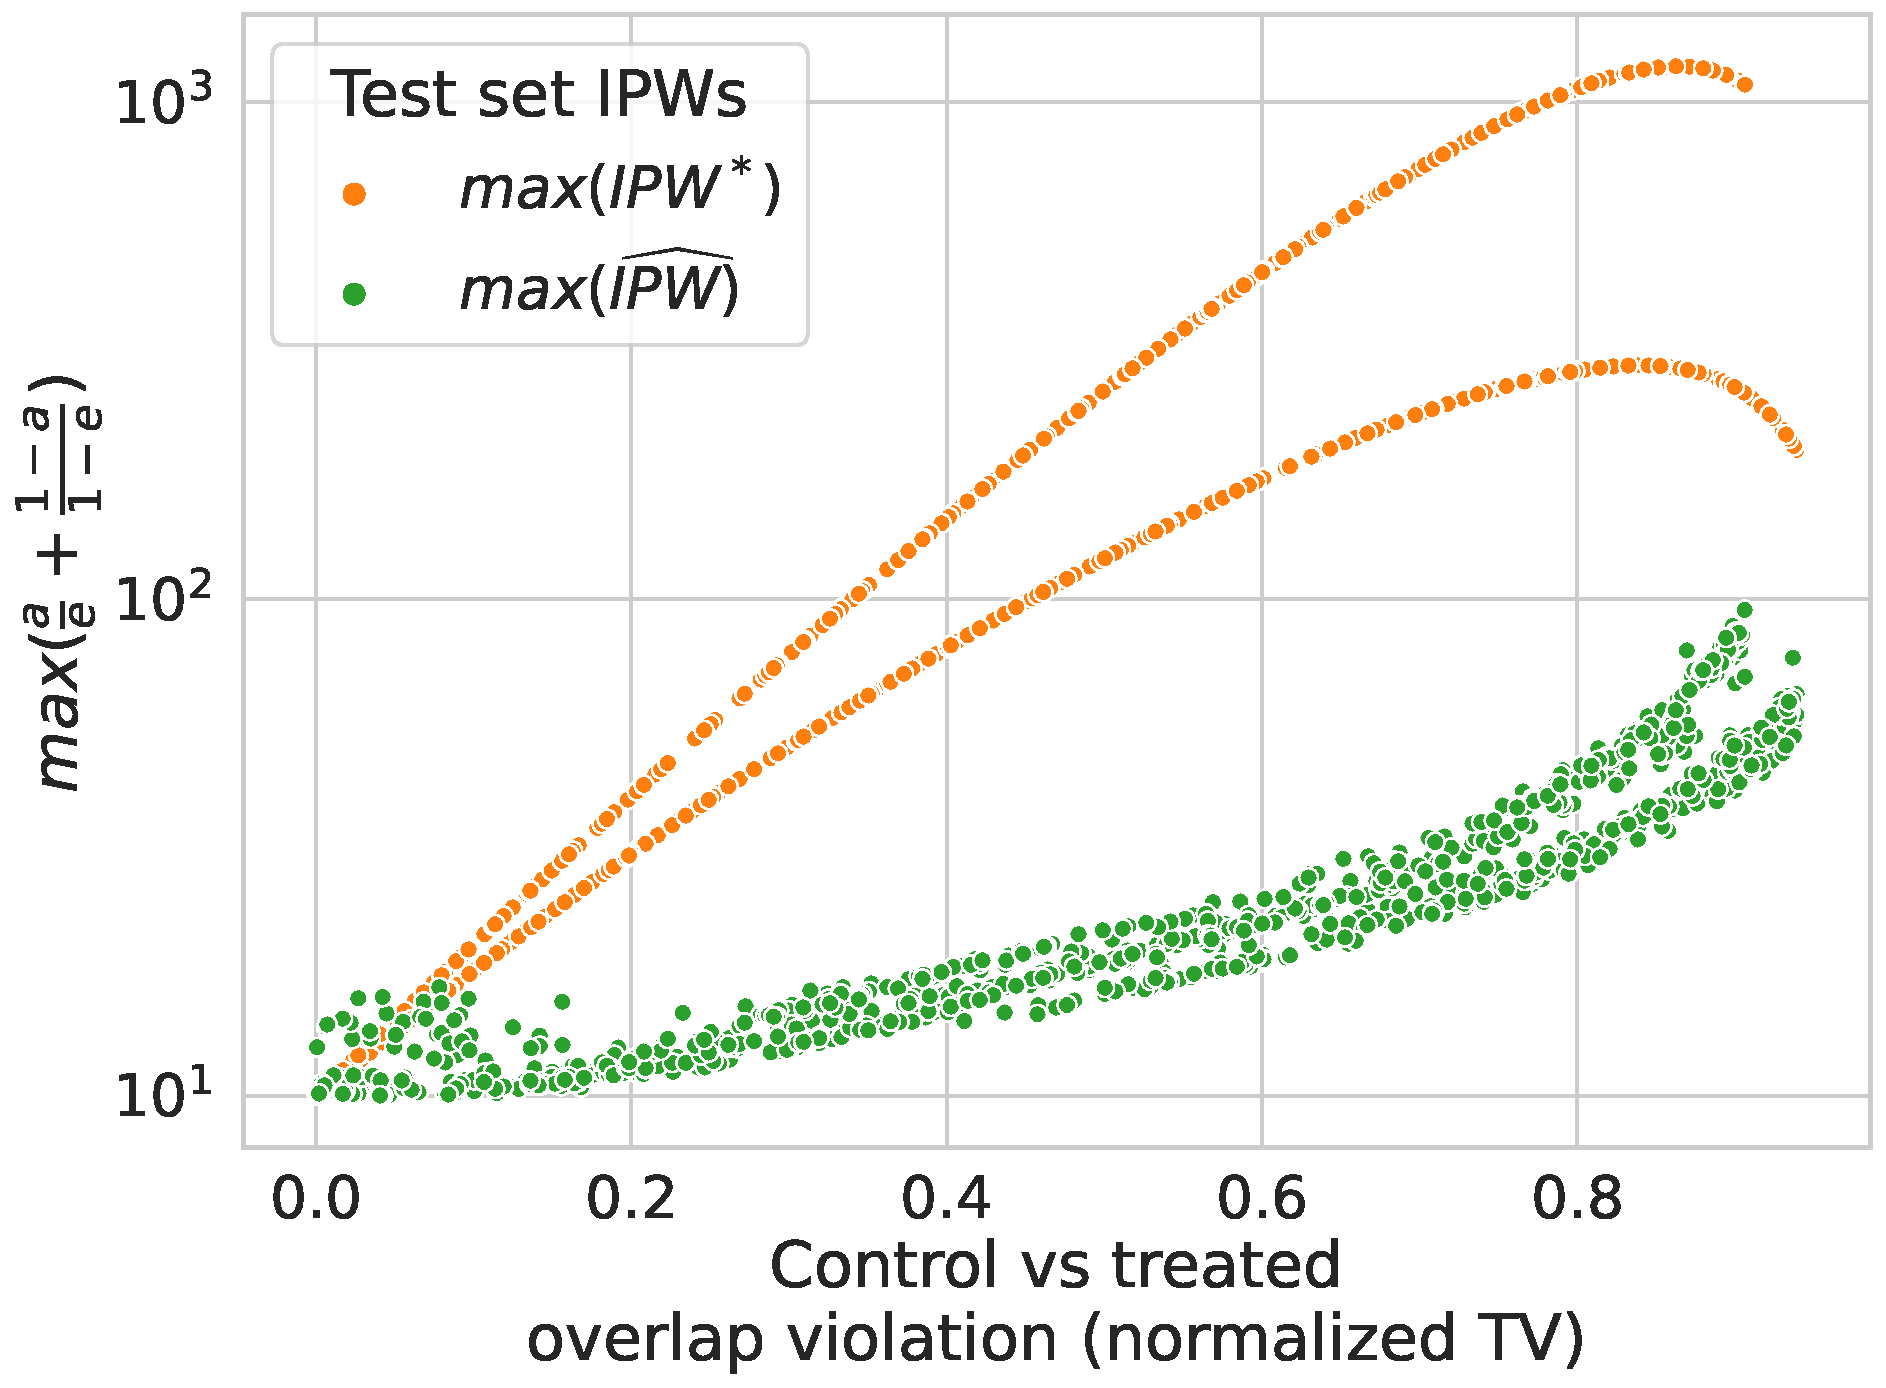
\includegraphics[width=\textwidth]{img/chapter_5/overlap_measure_caussim_max_ipw_vs_ntv.pdf}
      \label{apd:caussim:max_ipw_vs_ntv}
    \end{subfigure}
    \hfill
    \begin{subfigure}[b]{0.47\textwidth}
      \centering
      \caption{\textbf{ACIC 2016}}
      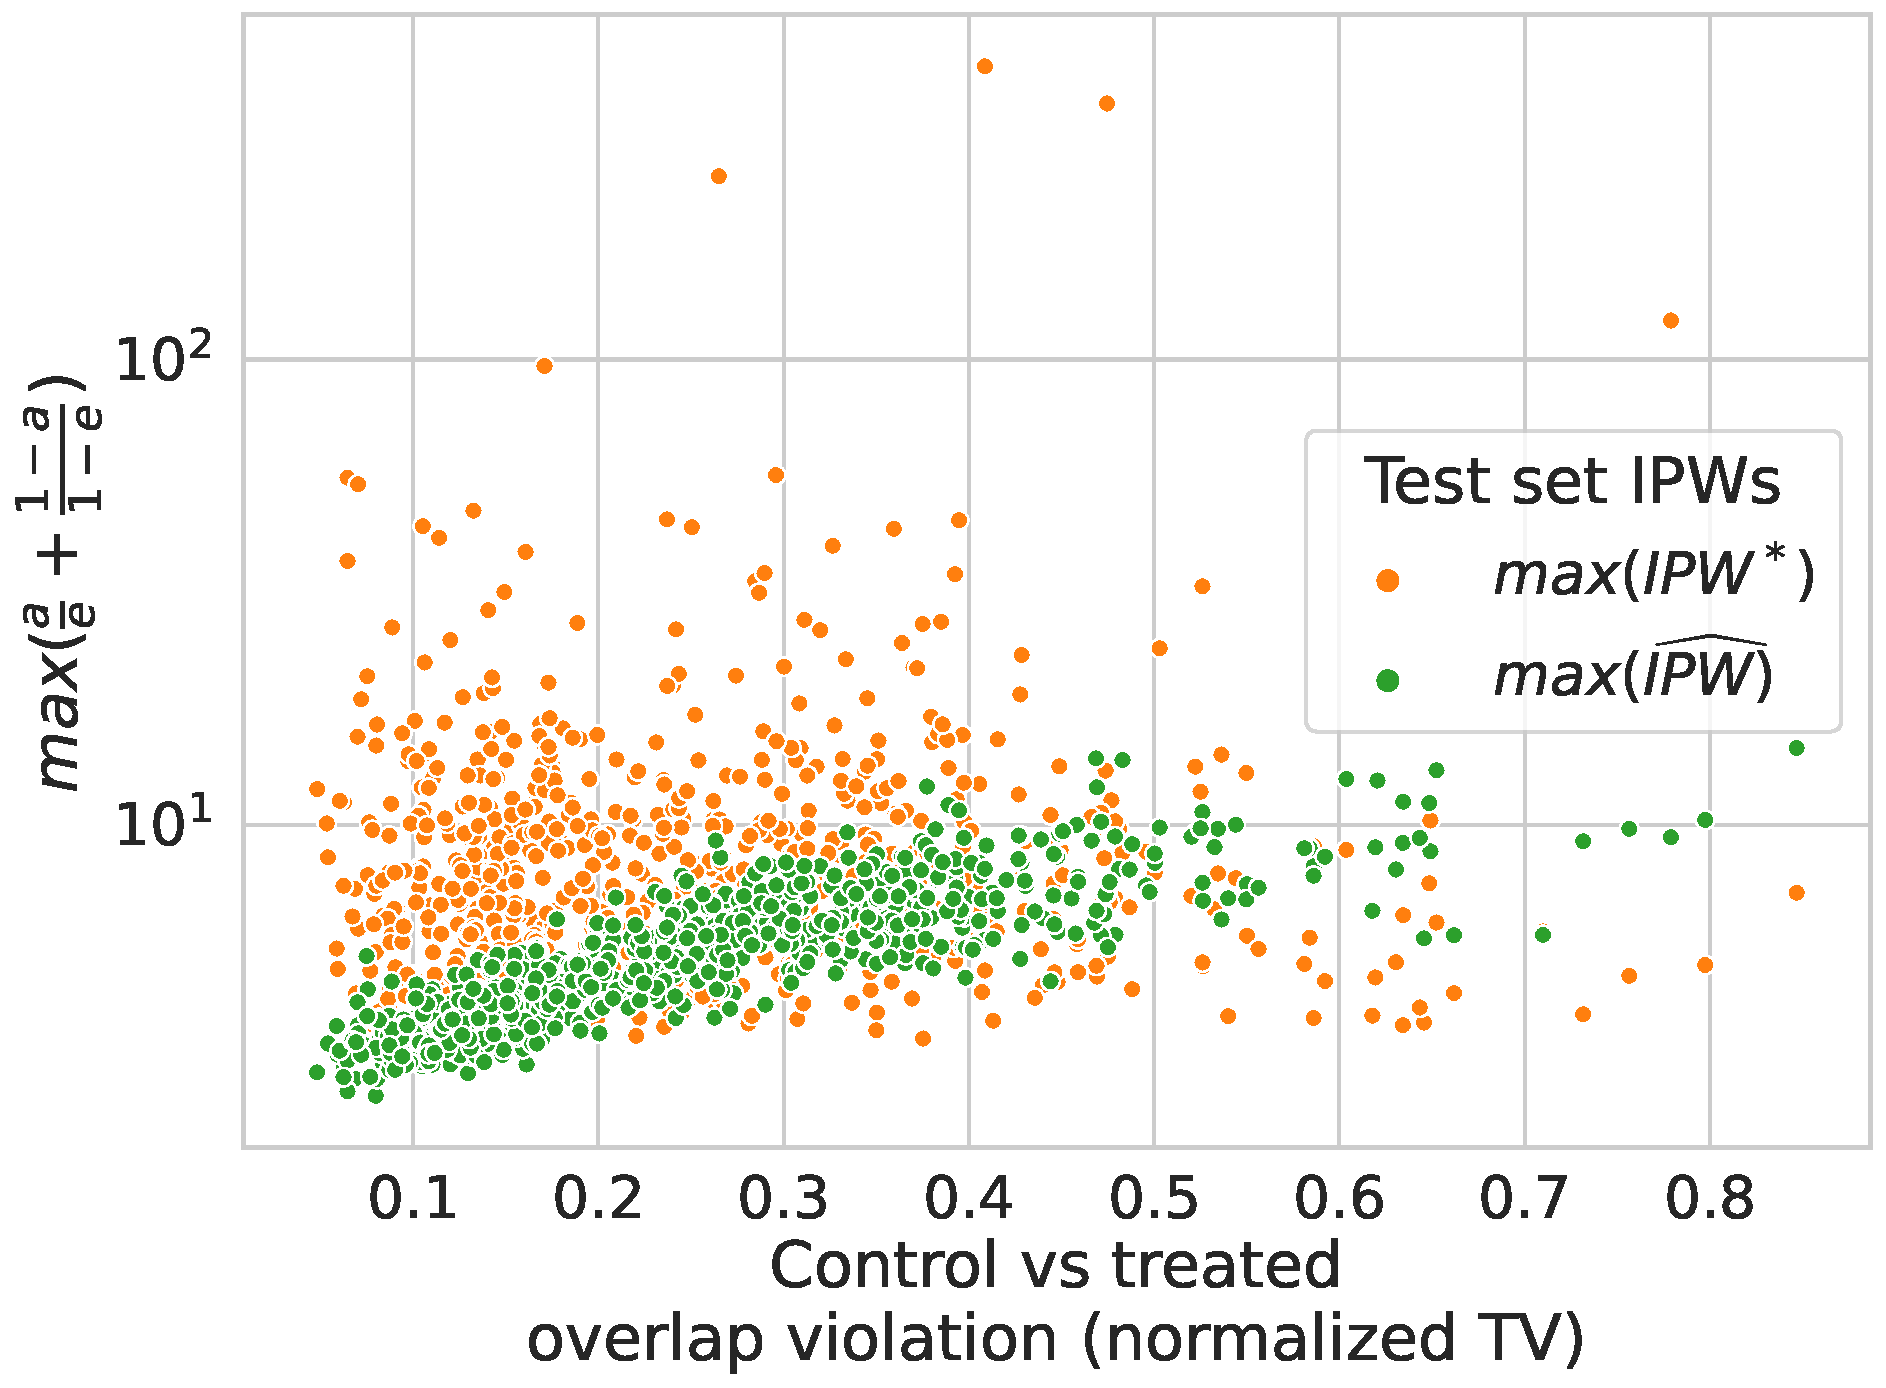
\includegraphics[width=\textwidth]{img/chapter_5/overlap_measure_acic_2016_max_ipw_vs_ntv.pdf}
      \label{apd:acic_2016:ntv_vs_max_ipw}
    \end{subfigure}
    \begin{subfigure}[b]{0.47\textwidth}
      \centering
      \caption{\textbf{ACIC 2018}}
      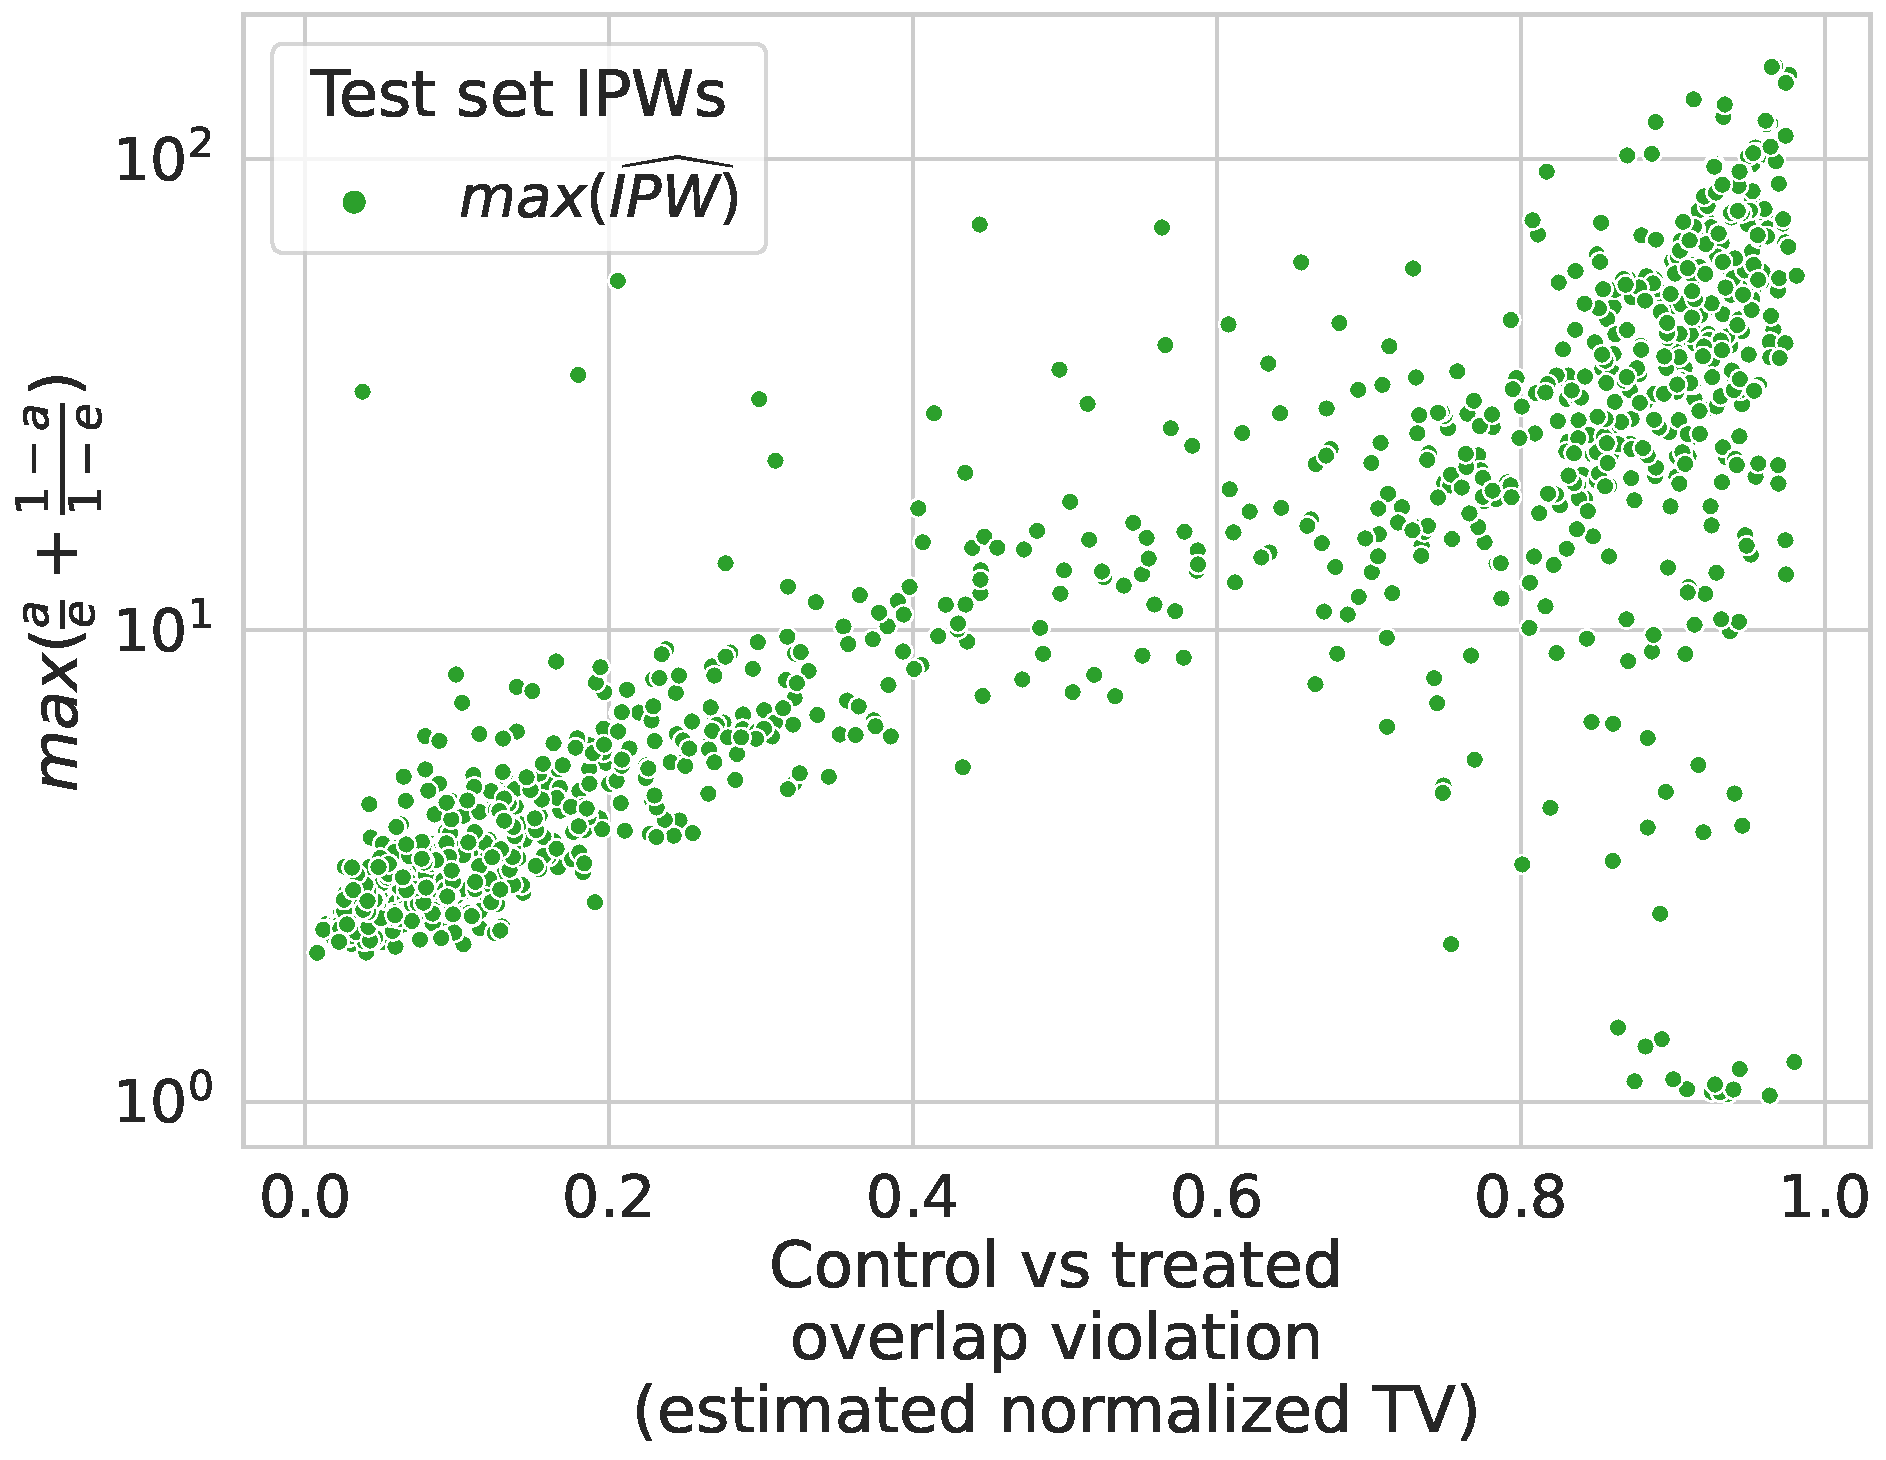
\includegraphics[width=\textwidth]{img/chapter_5/overlap_measure_acic_2018_max_ipw_vs_ntv.pdf}
      \label{apd:acic_2018:ntv_vs_max_ipw}
    \end{subfigure}
    \hfill
    \begin{subfigure}[b]{0.49\textwidth}
      \centering
      \caption{\textbf{TWINS}}
      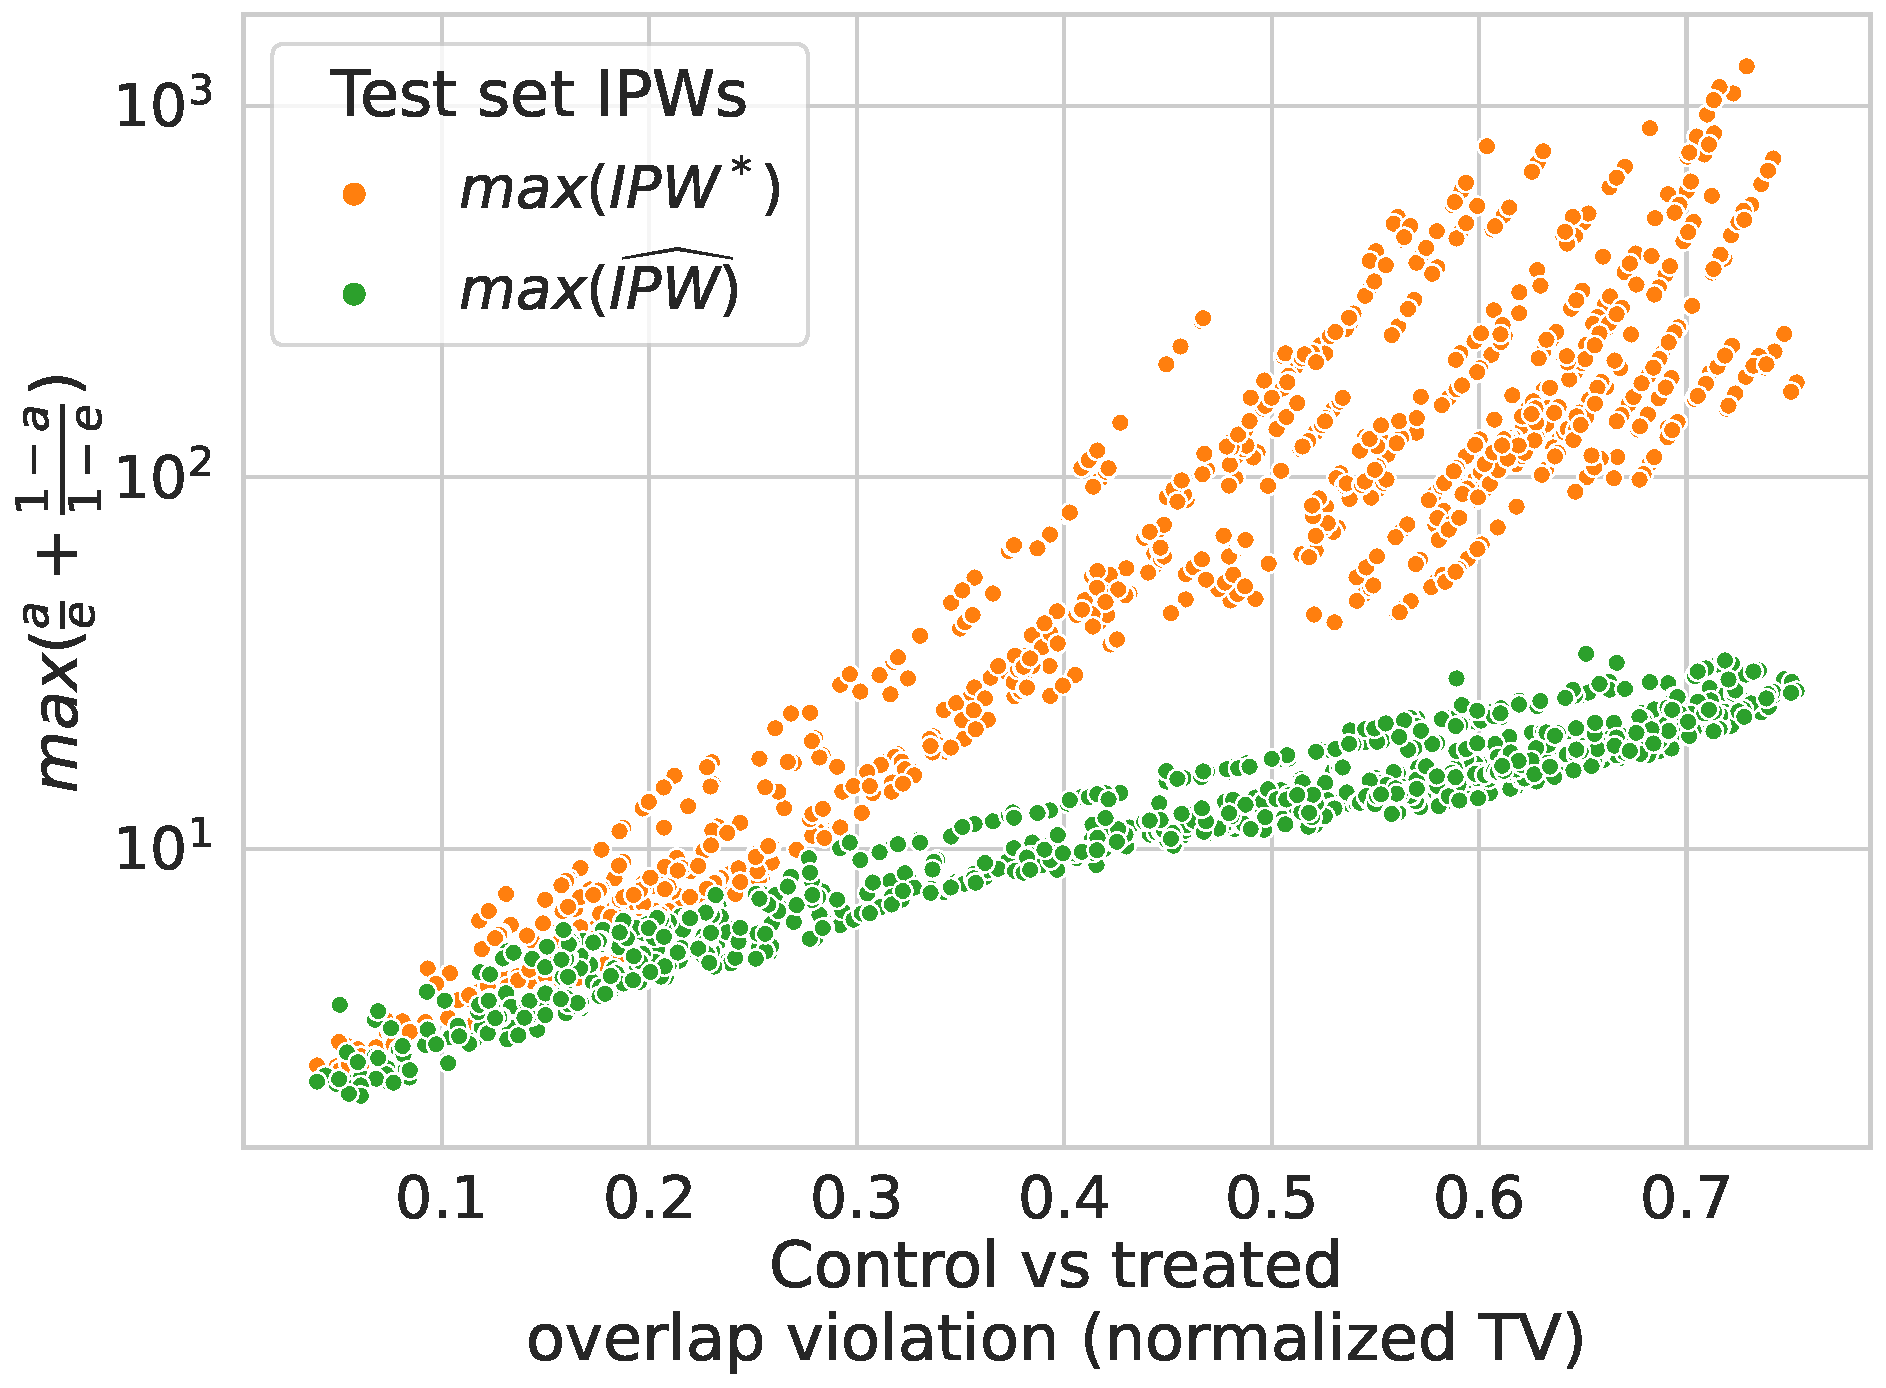
\includegraphics[width=\textwidth]{img/chapter_5/overlap_measure_twins_max_ipw_vs_ntv.pdf}
      \label{apd:twins:ntv_vs_max_ipw}
    \end{subfigure}
    \caption{Maximal value of Inverse Propensity Weights increases exponentially with the overlap as measure by Normalized Total Variation.}
    \label{apd:ntv_vs_max_ipw}
  \end{figure}

  \section{Experiments}

  \subsection{Details on the data generation process}
  \label{apd:experiments:generation}

  We use Gaussian-distributed covariates and random basis expansion based on
  Radial Basis Function kernels. A random basis of RBF kernel enables modeling
  non-linear and complex relationships between covariates in a similar way to the
  well known spline expansion. The estimators of the response function are learned
  with a linear model on another random basis (which can be seen as a stochastic
  approximation of the full data kernel \citep{rahimi_random_2008}). We
  carefully control the overlap between treated and control populations,
  a crucial assumption for causal inference.

  \begin{itemize}
    \item The raw features for both populations are drawn from a mixture of
          Gaussians:
          $\mathbb P(X) = p_A \mathbb P(X|A=1) + (1- p_A) \mathbb P(X|A=0)$
          where $\mathbb P(x|A=a)$ is a rotated Gaussian:
          \begin{equation}
            \mathbb P(x|A=a) = W \cdot \mathcal N \Big( \begin{bmatrix} (1-2a) \theta \\ 0\end{bmatrix} ; \begin{bmatrix} \sigma_0 & 0 \\ 0 & \sigma_1\end{bmatrix} \Big)
          \end{equation}
          with $\theta$ a parameter controlling overlap (bigger yields poorer
          overlap), $W$ a random rotation matrix and $\sigma_0^2=2;\sigma_1^2=5$.

          This generation process allows to analytically compute the oracle
          propensity scores $e(x)$, to simply control for overlap with the
          parameter $\theta$, the distance between the two Gaussian main axes and
          to  visualize response surfaces.

    \item A basis expansion of the raw features increases the problem dimension.
          Using Radial Basis Function (RBF) Nystroem transformation \footnote{We use the
            \href{https://scikit-learn.org/stable/modules/generated/sklearn.kernel_approximation.Nystroem.html}{Sklearn
              implementation, \citep{pedregosa_scikitlearn_2011}}}, we expand the raw
          features into a transformed space. The basis expansion samples randomly a
          small number of representers in the raw data. Then,  it computes an
          approximation of the full N-dimensional kernel with these basis components,
          yielding the transformed features $z(x)$.

          We generate the basis following the original data distribution, $\left [
              b_1 .. b_D \right ] \sim \mathbb P(x)$, with D=2 in our simulations. Then, we
          compute an approximation of the full kernel of the data generation
          process $RBF(x, \cdot) \;  with \; x \sim \mathbb P(x)$ with these
          representers: $z(x) = [RBF_{\gamma}(x, b_d)]_{d=1..D}
            \cdot Z^T \in \mathbb{R}^D$
          with $RBF_{\gamma}$ being the Gaussian kernel $K(x, y) = exp(-\gamma
            ||x-y||^2)$ and Z the normalization constant of the kernel basis,
          computed as the root inverse of the basis kernel $Z=[K(b_i, b_j)]_{i, j
            \in {1..D}}^{-1/2}$


    \item Functions $\mu_0$, $\tau$ are distinct linear functions of the
          transformed features:
          \begin{equation*}
            \mu_0(x) = \begin{bmatrix} z(x); 1 \end{bmatrix} \cdot \beta_{\mu}^T
          \end{equation*}
          \begin{equation*}
            \tau(x) = \begin{bmatrix} z(x); 1 \end{bmatrix} \cdot \beta_{\tau}^T
          \end{equation*}
    \item Adding a Gaussian noise, $\varepsilon \sim \mathcal N(0, \sigma(x;a))$,
          we construct the potential outcomes:
          $y(a) = \mu_0(x) + a\,\tau(x) + \varepsilon(x, a)$
  \end{itemize}
  We generated 1000 instances of this dataset with uniformly random overlap
  parameters $\theta \in \left[ 0, 2.5 \right]$.

  \subsection{Model selection procedures}

  \paragraph{Nuisances estimation}\label{apd:experiments:nuisances_hp}

  The nuisances are estimated with a stacked regressor inspired by the Super
  Learner framework, \citep{laan_super_2007}. The hyper-parameters are
  optimized with a random search with following search grid detailed in Table
  \ref{apd:experiments:nuisances_hp_grid}. All implementations come from
  \href{https://scikit-learn.org/stable/}{scikit-learn}
  \citep{pedregosa_scikitlearn_2011}.

  \begin{table}[h!]
    \begin{tabular}{llll}
      \toprule
      Model                & Estimator
                           & Hyper-parameters grid                                         \\
      \midrule
      Outcome, m           & StackedRegressor
                           & ridge regularization: [0.0001, 0.001, 0.01, 0.1, 1, 10, 100]  \\
      \multirow[c]{3}{*}{} & (HistGradientBoostingRegressor, ridge)
                           & HistGradientBoostingRegressor  learning rate: [0.01, 0.1, 1]  \\
                           &
                           & HistGradientBoostingRegressor  max leaf nodes: [10,
      20, 30, 50]                                                                          \\
      \midrule
      Treatment, e         & StackedClassifier
                           & LogisticRegression  C: [0.0001, 0.001, 0.01, 0.1, 1, 10, 100] \\
      \multirow[c]{3}{*}{} & (HistgradientBoostingClassifier, LogisticRegression)
                           & HistGradientBoostingClassifier  learning rate: [0.01, 0.1, 1] \\
                           &
                           & HistGradientBoostingClassifier  max leaf nodes: [10,
      20, 30, 50]                                                                          \\
      \bottomrule
    \end{tabular}
    \caption{Hyper-parameters grid used for nuisance models}
    \label{apd:experiments:nuisances_hp_grid}
  \end{table}


  \subsection{Additional Results}\label{apd:experiments:additional_results}

  \paragraph{Definition of the Kendall's tau, $\kappa$}

  The Kendall's tau  is a widely used statistics to measure the rank correlation
  between two set of observations. It measures the number of concordant pairs
  minus the discordant pairs normalized by the total number of pairs. It takes values in the
  $[-1, 1]$ range.
  \begin{equation}\label{eq:kendall_tau}
    \kappa=\frac{\text { (number of concordant pairs })-\text { (number of discordant pairs) }}{\text { (number of pairs) }}
  \end{equation}

  \paragraph{Values of relative $\kappa(\ell,\tau\mathrm{{-risk}})$ compared to
    the mean over all metrics Kendall's as shown in the boxplots of Figure \ref{fig:relative_kendalls_all_datasets}}

  \begin{table}
    \centering
    \resizebox{0.7\textwidth}{!}{
      \begin{tabular}{llrrrr}
\toprule
 &  & \multicolumn{2}{r}{Strong Overlap} & \multicolumn{2}{r}{Weak Overlap} \\
 &  & Median & IQR & Median & IQR \\
Metric & Dataset &  &  &  &  \\
\midrule
\multirow[c]{4}{*}{$\widehat{\mu\mathrm{-risk}}$} & Twins 
 (N= 11 984) & -0.32 & 0.12 & -0.19 & 0.12 \\
\cline{2-6}
 & ACIC 2016
 (N=4 802) & -0.03 & 0.13 & 0.11 & 0.19 \\
\cline{2-6}
 & Caussim
 (N=5 000) & -0.40 & 0.55 & -0.16 & 0.31 \\
\cline{2-6}
 & ACIC 2018 
 (N=5 000) & 0.00 & 0.30 & 0.01 & 0.40 \\
\cline{1-6} \cline{2-6}
\multirow[c]{4}{*}{$\widehat{\mu\mathrm{-risk}}_{IPW}$} & Twins 
 (N= 11 984) & -0.31 & 0.13 & -0.17 & 0.12 \\
\cline{2-6}
 & ACIC 2016
 (N=4 802) & -0.02 & 0.13 & 0.11 & 0.19 \\
\cline{2-6}
 & Caussim
 (N=5 000) & -0.34 & 0.50 & 0.09 & 0.31 \\
\cline{2-6}
 & ACIC 2018 
 (N=5 000) & 0.00 & 0.30 & -0.01 & 0.43 \\
\cline{1-6} \cline{2-6}
\multirow[c]{3}{*}{$\widehat{\mu\mathrm{-risk}}^{*}_{IPW}$} & Twins 
 (N= 11 984) & -0.32 & 0.13 & -0.17 & 0.13 \\
\cline{2-6}
 & ACIC 2016
 (N=4 802) & -0.02 & 0.13 & 0.11 & 0.21 \\
\cline{2-6}
 & Caussim
 (N=5 000) & -0.33 & 0.54 & 0.26 & 0.27 \\
\cline{1-6} \cline{2-6}
\multirow[c]{4}{*}{$\widehat{\tau\mathrm{-risk}}_{IPW}$} & Twins 
 (N= 11 984) & 0.13 & 0.12 & 0.27 & 0.12 \\
\cline{2-6}
 & ACIC 2016
 (N=4 802) & -0.07 & 0.18 & 0.05 & 0.31 \\
\cline{2-6}
 & Caussim
 (N=5 000) & -0.19 & 0.43 & -0.14 & 0.18 \\
\cline{2-6}
 & ACIC 2018 
 (N=5 000) & -0.16 & 0.40 & -0.11 & 0.66 \\
\cline{1-6} \cline{2-6}
\multirow[c]{3}{*}{$\widehat{\tau\mathrm{-risk}}_{IPW}^{*}$} & Twins 
 (N= 11 984) & 0.12 & 0.14 & 0.20 & 0.16 \\
\cline{2-6}
 & ACIC 2016
 (N=4 802) & -0.03 & 0.16 & -0.09 & 0.43 \\
\cline{2-6}
 & Caussim
 (N=5 000) & -0.15 & 0.46 & -0.17 & 0.19 \\
\cline{1-6} \cline{2-6}
\multirow[c]{4}{*}{$\widehat{\mathrm{U-risk}}$} & Twins 
 (N= 11 984) & 0.13 & 0.12 & 0.02 & 0.25 \\
\cline{2-6}
 & ACIC 2016
 (N=4 802) & 0.04 & 0.11 & 0.11 & 0.26 \\
\cline{2-6}
 & Caussim
 (N=5 000) & 0.04 & 0.43 & -0.04 & 0.17 \\
\cline{2-6}
 & ACIC 2018 
 (N=5 000) & 0.12 & 0.26 & -0.02 & 0.50 \\
\cline{1-6} \cline{2-6}
\multirow[c]{3}{*}{$\widehat{\mathrm{U-risk}}^{*}$} & Twins 
 (N= 11 984) & 0.25 & 0.08 & -0.41 & 0.45 \\
\cline{2-6}
 & ACIC 2016
 (N=4 802) & 0.08 & 0.13 & -0.59 & 0.57 \\
\cline{2-6}
 & Caussim
 (N=5 000) & 0.46 & 0.12 & 0.02 & 0.44 \\
\cline{1-6} \cline{2-6}
\multirow[c]{4}{*}{$\widehat{\mathrm{R-risk}}$} & Twins 
 (N= 11 984) & 0.15 & 0.10 & 0.25 & 0.18 \\
\cline{2-6}
 & ACIC 2016
 (N=4 802) & 0.07 & 0.12 & 0.22 & 0.15 \\
\cline{2-6}
 & Caussim
 (N=5 000) & 0.34 & 0.26 & 0.13 & 0.21 \\
\cline{2-6}
 & ACIC 2018 
 (N=5 000) & 0.13 & 0.27 & 0.21 & 0.47 \\
\cline{1-6} \cline{2-6}
\multirow[c]{3}{*}{$\widehat{\mathrm{R-risk}}^{*}$} & Twins 
 (N= 11 984) & 0.25 & 0.10 & 0.32 & 0.15 \\
\cline{2-6}
 & ACIC 2016
 (N=4 802) & 0.12 & 0.12 & 0.25 & 0.15 \\
\cline{2-6}
 & Caussim
 (N=5 000) & 0.47 & 0.11 & 0.16 & 0.14 \\
\cline{1-6} \cline{2-6}
\bottomrule
\end{tabular}

    }
    \caption{Values of relative $\kappa(\ell,\tau\mathrm{{-risk}})$ compared to
      the mean over all metrics Kendall's as shown in the boxplots of Figure
      \ref{fig:relative_kendalls_all_datasets}}\label{apd:table:relative_kendalls_all_datasets}
  \end{table}


  \paragraph{Figure \ref{apd:fig:relative_kendalls_all_datasets_all_metrics} -
    Results measured in relative Kendall's for feasible and semi-oracle risks}

  Because of extreme propensity scores in the denominator and bayes error residuals in the numerator, the semi-oracle
  $U$-risk has poor performances at bad overlap. Estimating these propensity scores in the is feasible $U$-risk reduces
  the variance since clipping is performed.

  \begin{figure}[!b]
    \centering
    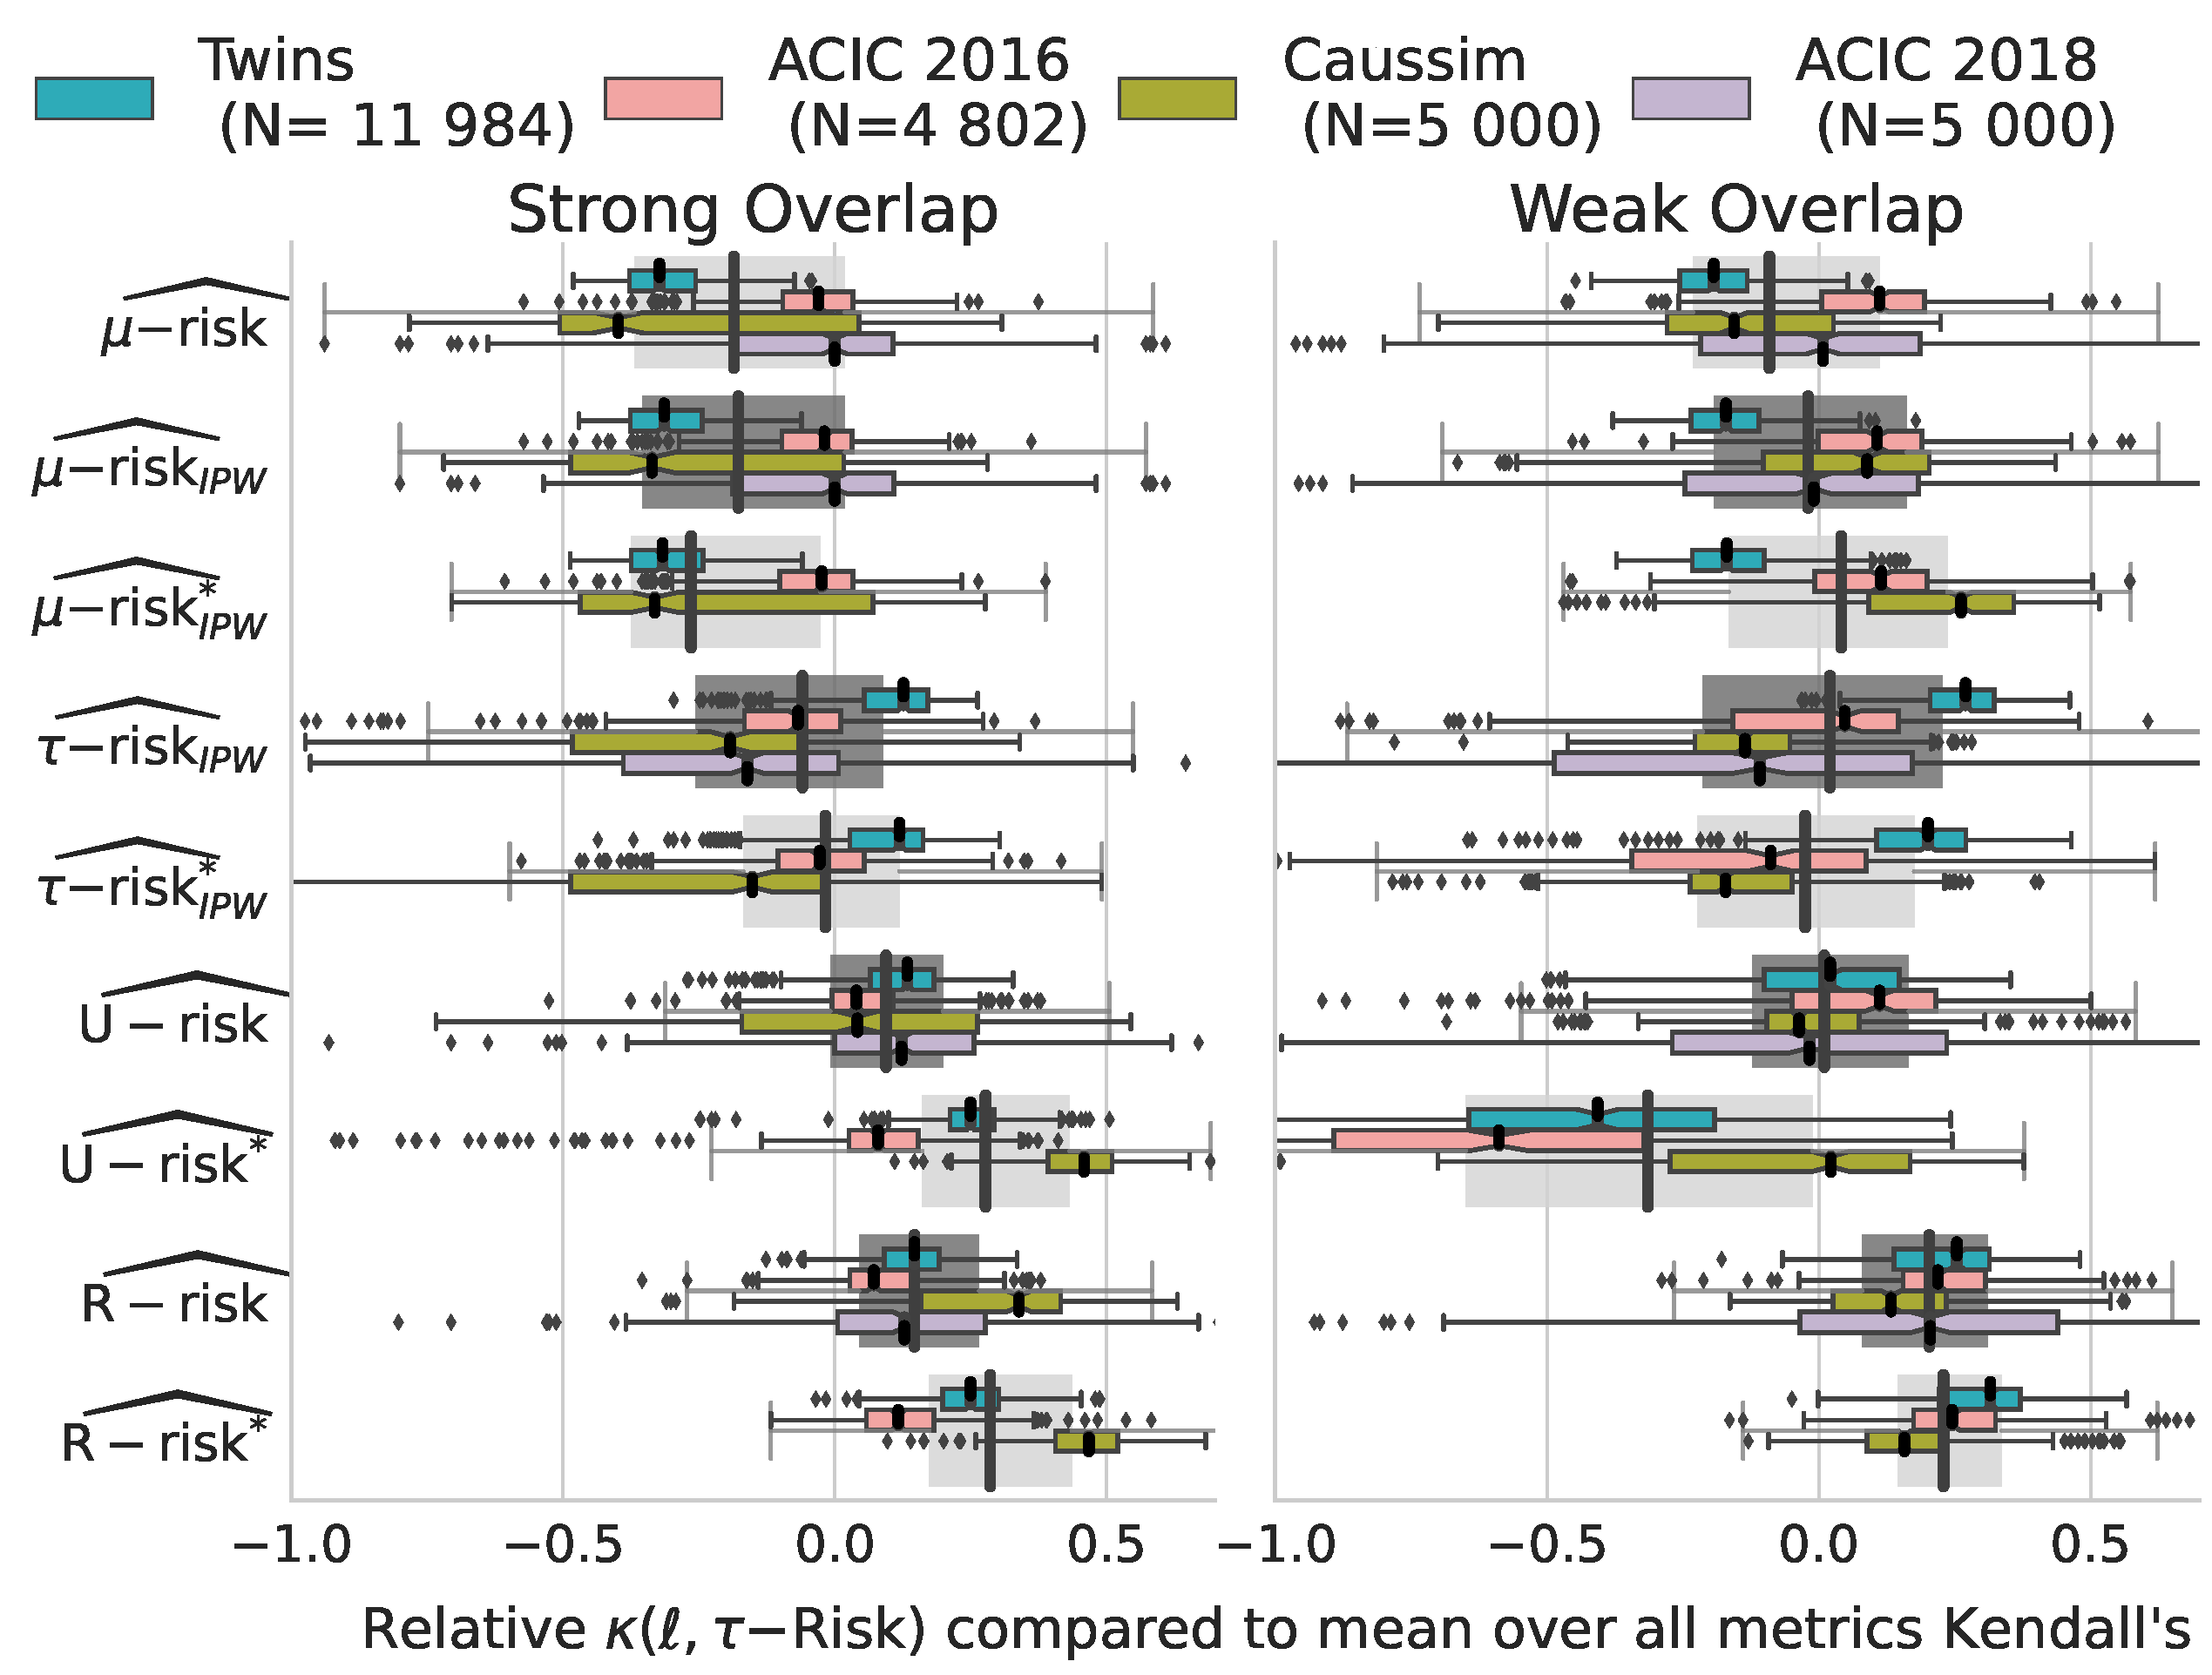
\includegraphics[width=\linewidth]{img/chapter_5/_1_r_risk_domination_r_risk_domination__ref_metric_mean_risks_by_Dataset.pdf}
    %\hfill
    \caption{\textbf{The $R$-risk is the best metric}: Relative Kendall's $\tau$
      agreement with $\tau\text{-risk}$. Strong and weak overlap correspond to
      the first and last tertiles of the overlap distribution measured with
      Normalized Total Variation eq. \ref{eq:ntv}.
    }\label{apd:fig:relative_kendalls_all_datasets_all_metrics}
  \end{figure}

  \paragraph{Figure \ref{apd:fig:all_datasets_tau_risk_ranking_agreement} -
    Results measured in absolute Kendall's}


  \begin{figure}
    \centering
    \begin{subfigure}[b]{0.44\textwidth}
      \centering
      \caption{\textbf{Caussim}}
      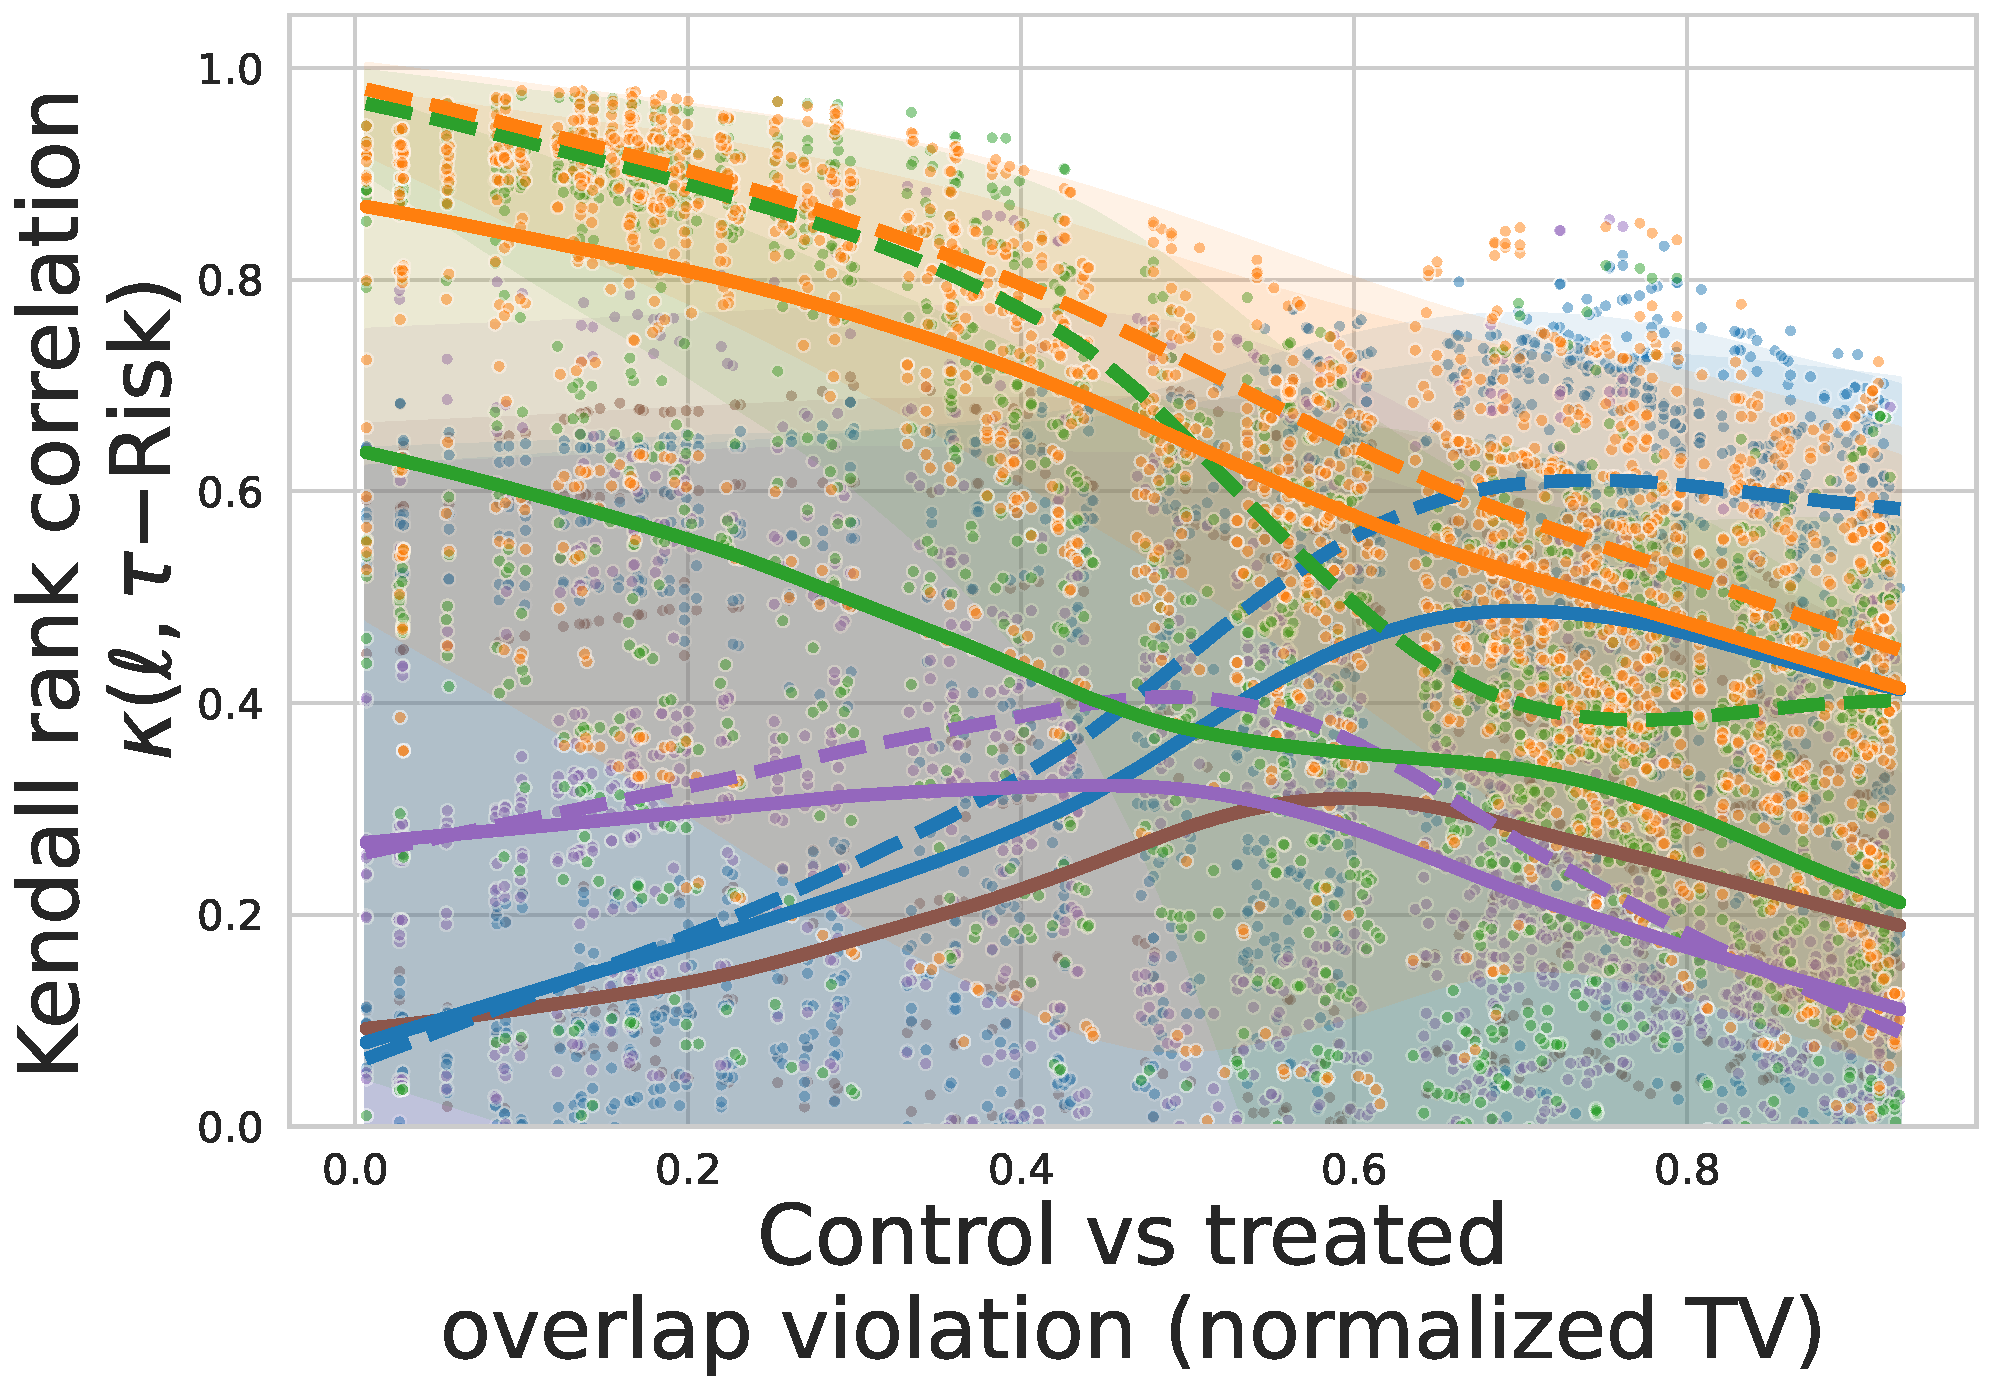
\includegraphics[width=\textwidth]{img/chapter_5/kendalls_tau_caussim__nuisance_non_linear__candidates_ridge__overlap_01-247.pdf}
      \label{fig:ranking_agreement_w_tau_risk_caussim}
    \end{subfigure}
    \hfill
    \begin{subfigure}[b]{0.44\textwidth}
      \centering
      \caption{\textbf{ACIC 2016}}
      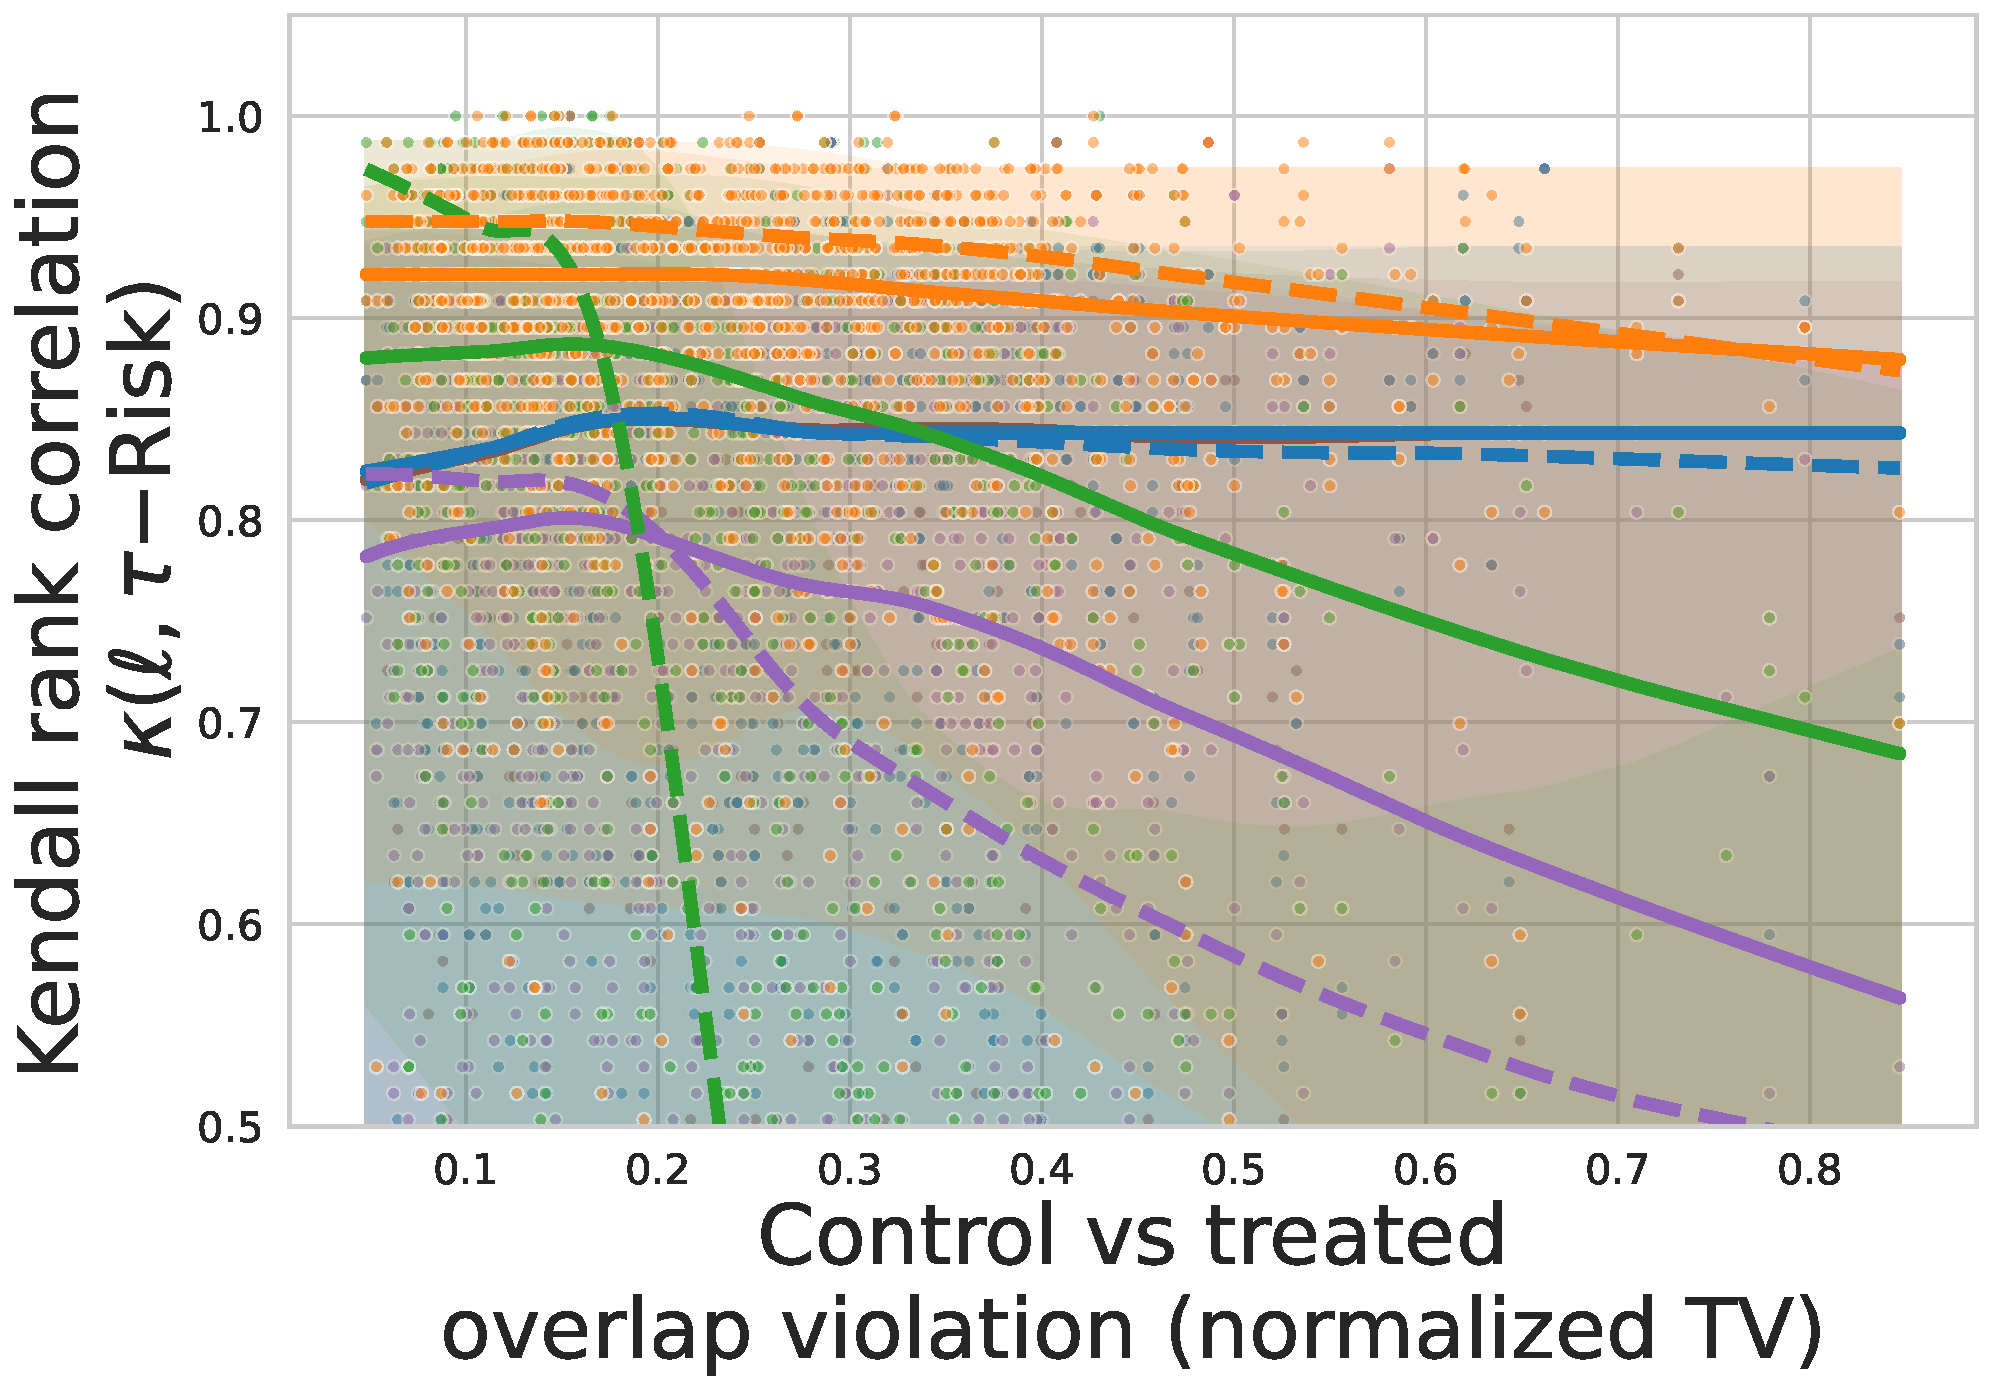
\includegraphics[width=\textwidth]{img/chapter_5/kendalls_tau_acic_2016__nuisance_non_linear__candidates_hist_gradient_boosting__dgp_1-77__rs_1-10.pdf}
      \label{fig:ranking_agreement_tau_risk_acic_2016}
    \end{subfigure}
    \hfill
    \begin{subfigure}[b]{0.10\textwidth}
      \centering
      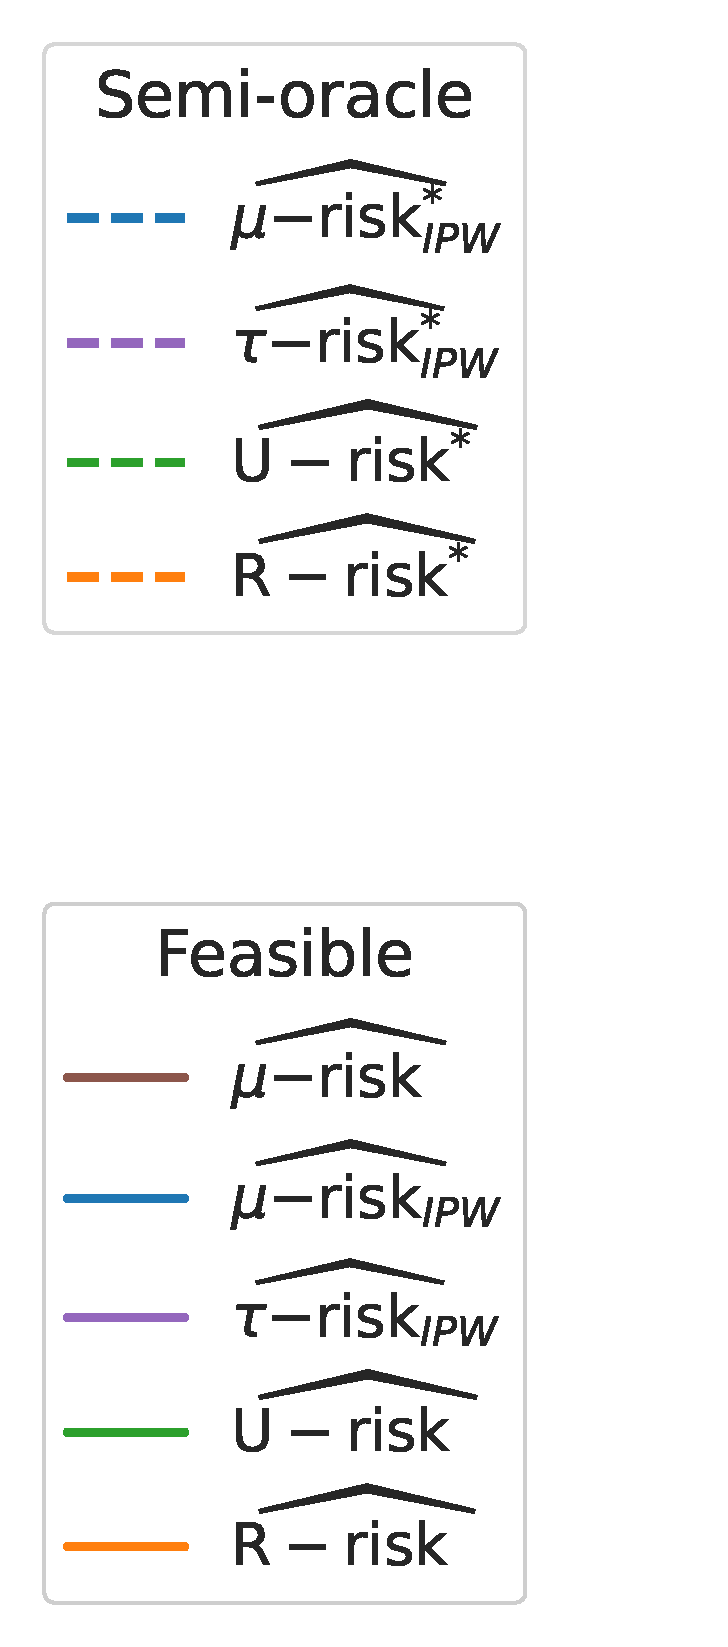
\includegraphics[width=1.5\textwidth]{img/chapter_5/legend_metrics.pdf}
    \end{subfigure}
    \begin{subfigure}[b]{0.44\textwidth}
      \centering
      \caption{\textbf{ACIC 2018}}
      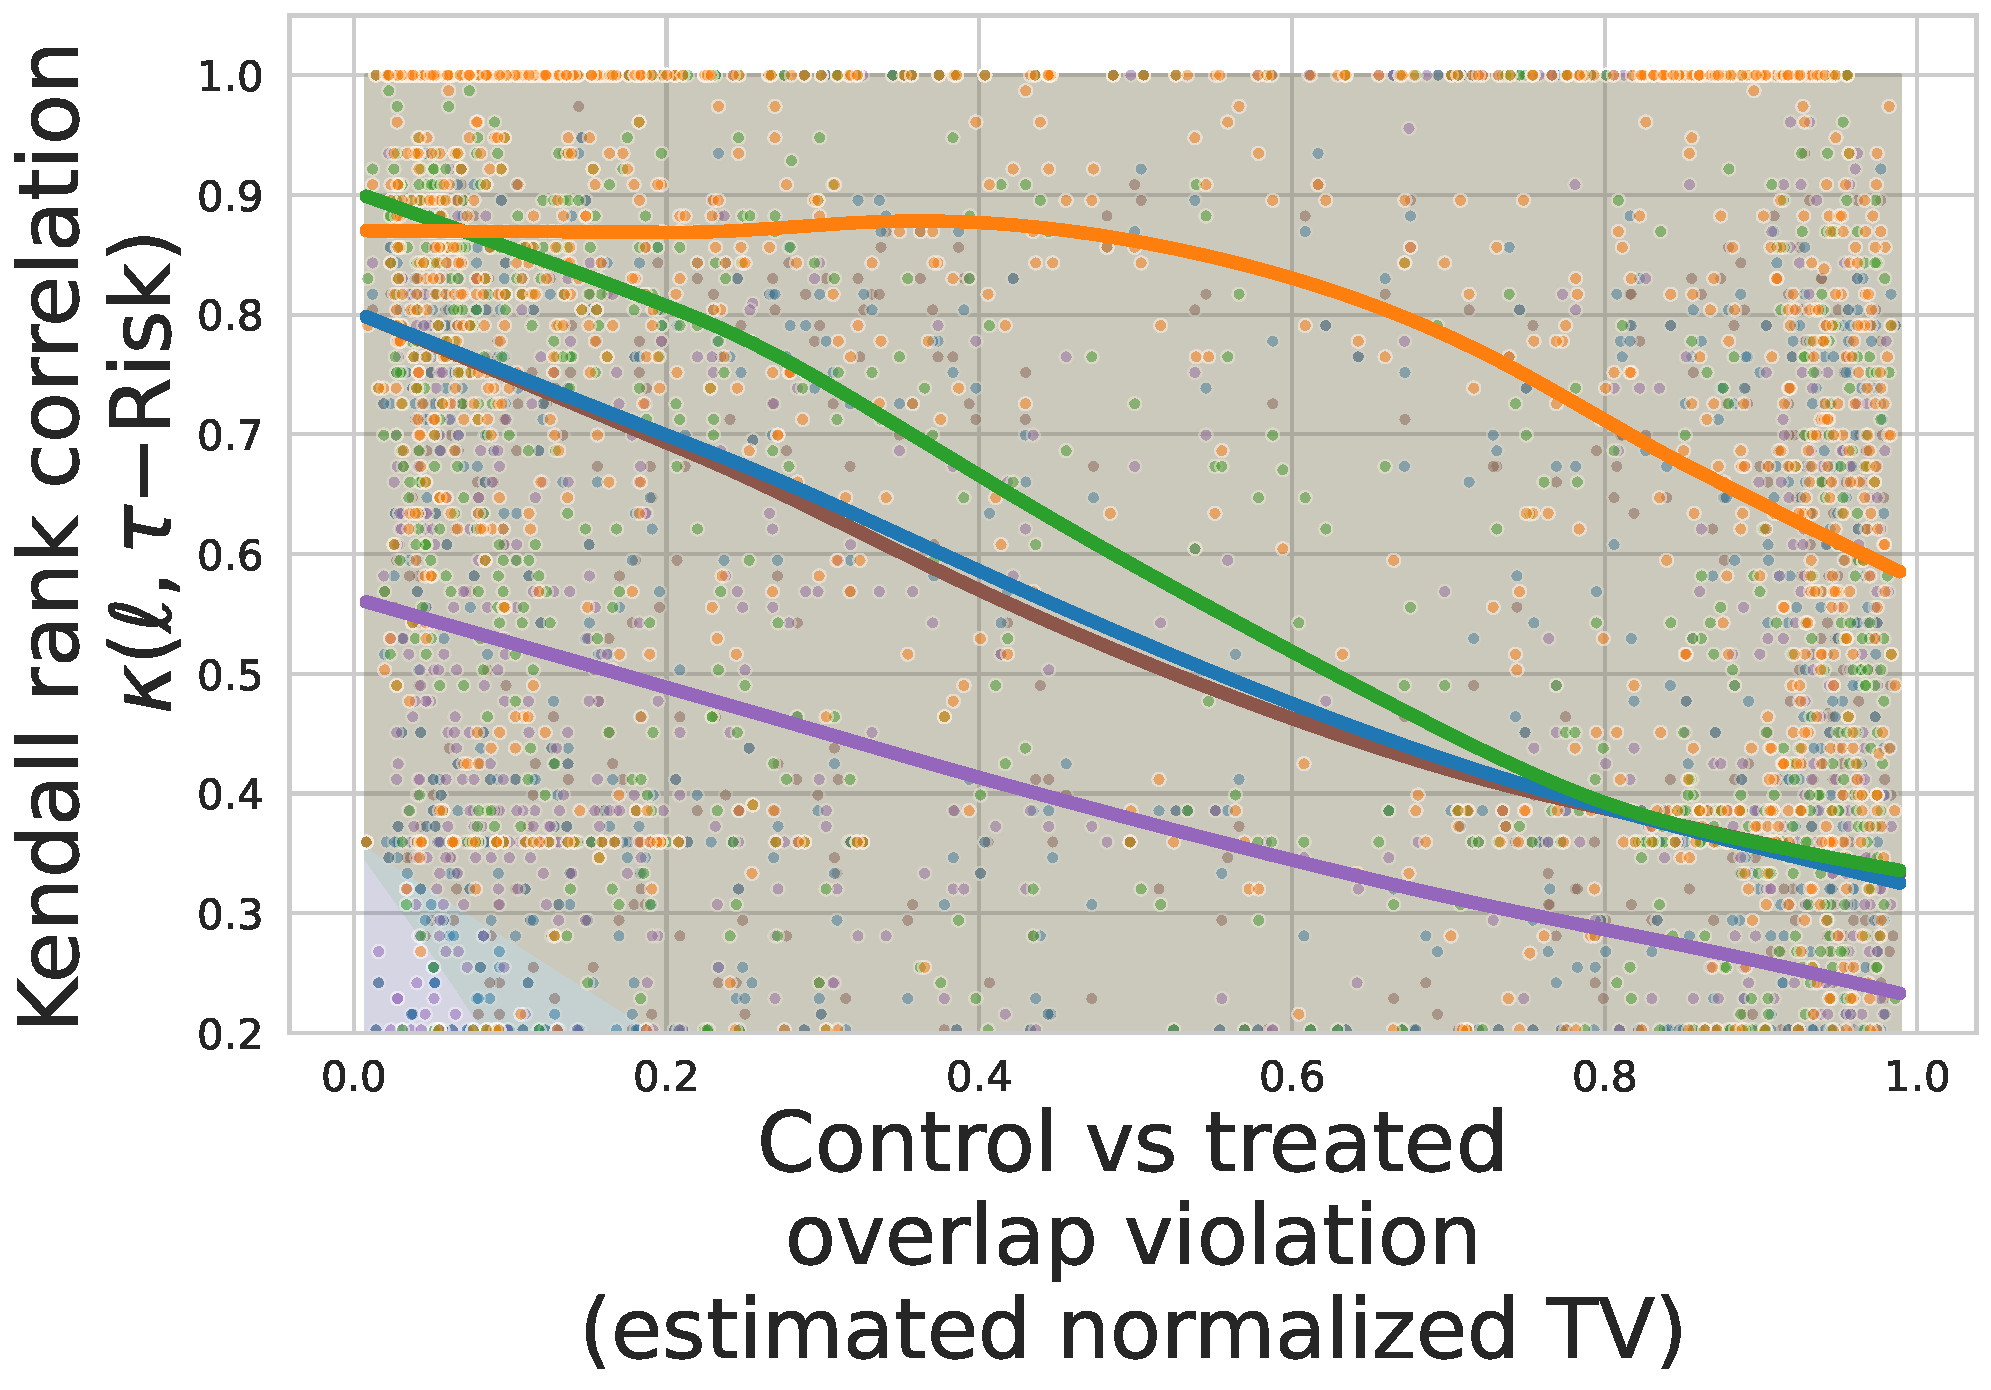
\includegraphics[width=\textwidth]{img/chapter_5/kendalls_tau_acic_2018__nuisance_stacking__candidates_hist_gradient_boosting__tset_50.pdf}
      \label{fig:ranking_agreement_w_tau_risk_acic_2018}
    \end{subfigure}
    \hfill
    \begin{subfigure}[b]{0.44\textwidth}
      \centering
      \caption{\textbf{TWINS}}
      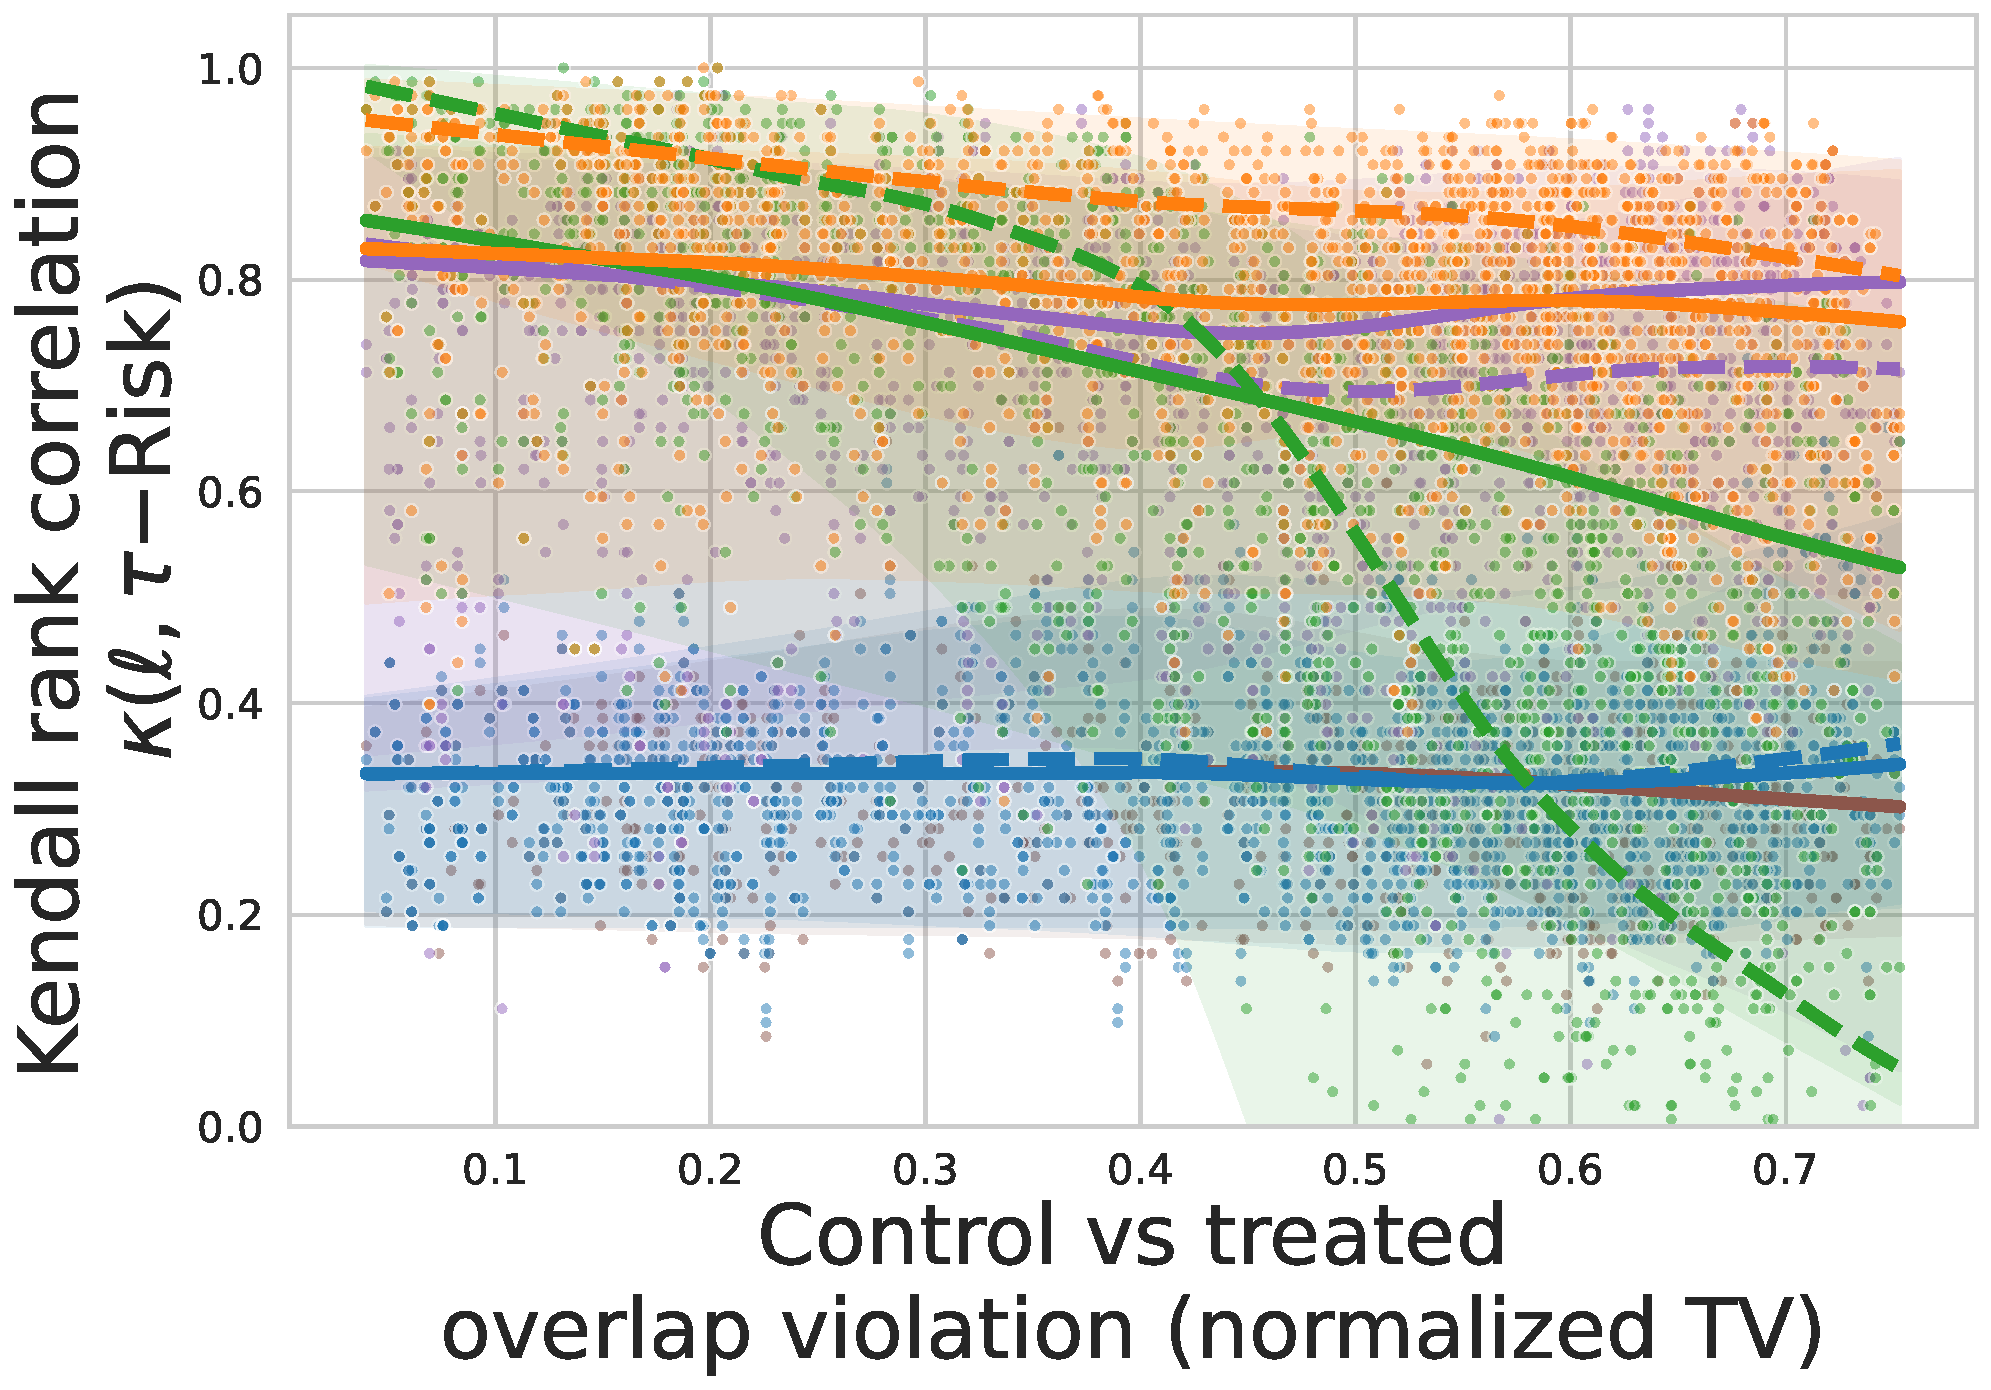
\includegraphics[width=\textwidth]{img/chapter_5/kendalls_tau_twins__nuisance_stacking__candidates_hist_gradient_boosting__tset_50__overlap_11-296__rs_0-9_noise10.pdf}
      \label{fig:ranking_agreement_tau_risk_twins}
    \end{subfigure}
    \hfill
    \begin{subfigure}[b]{0.10\textwidth}
      ~
    \end{subfigure}
    % \begin{subfigure}[b]{\textwidth}
    %   \centering
    %   \includegraphics[width=0.5\textwidth]{img/chapter_5/legend_metrics_horizontal.pdf}
    % \end{subfigure}
    \caption{Agreement with $\tau\text{-risk}$ ranking of methods function
      of overlap violation. The lines represent medians, estimated with a
      lowess. The transparent
      bands denote the 5\% and 95\% confidence intervals.}\label{apd:fig:all_datasets_tau_risk_ranking_agreement}
  \end{figure}



  \paragraph{Figure \ref{apd:all_datasets_normalized_bias_tau_risk_to_best_method}
    - Results measured as distance to the oracle tau-risk}

  To see practical gain in term of $\tau\text{-risk}$, we plot the results as the
  normalized distance between the estimator selected by the oracle
  $\tau\text{-risk}$ and the estimator selected by each causal metric.

  Then, $\widehat{R\text{-risk}}^*$ is more efficient than all other metrics. The
  gain are substantial for every datasets.

  \begin{figure}
    \centering
    \begin{subfigure}[b]{0.44\textwidth}
      \centering
      \caption{\textbf{Caussim}}
      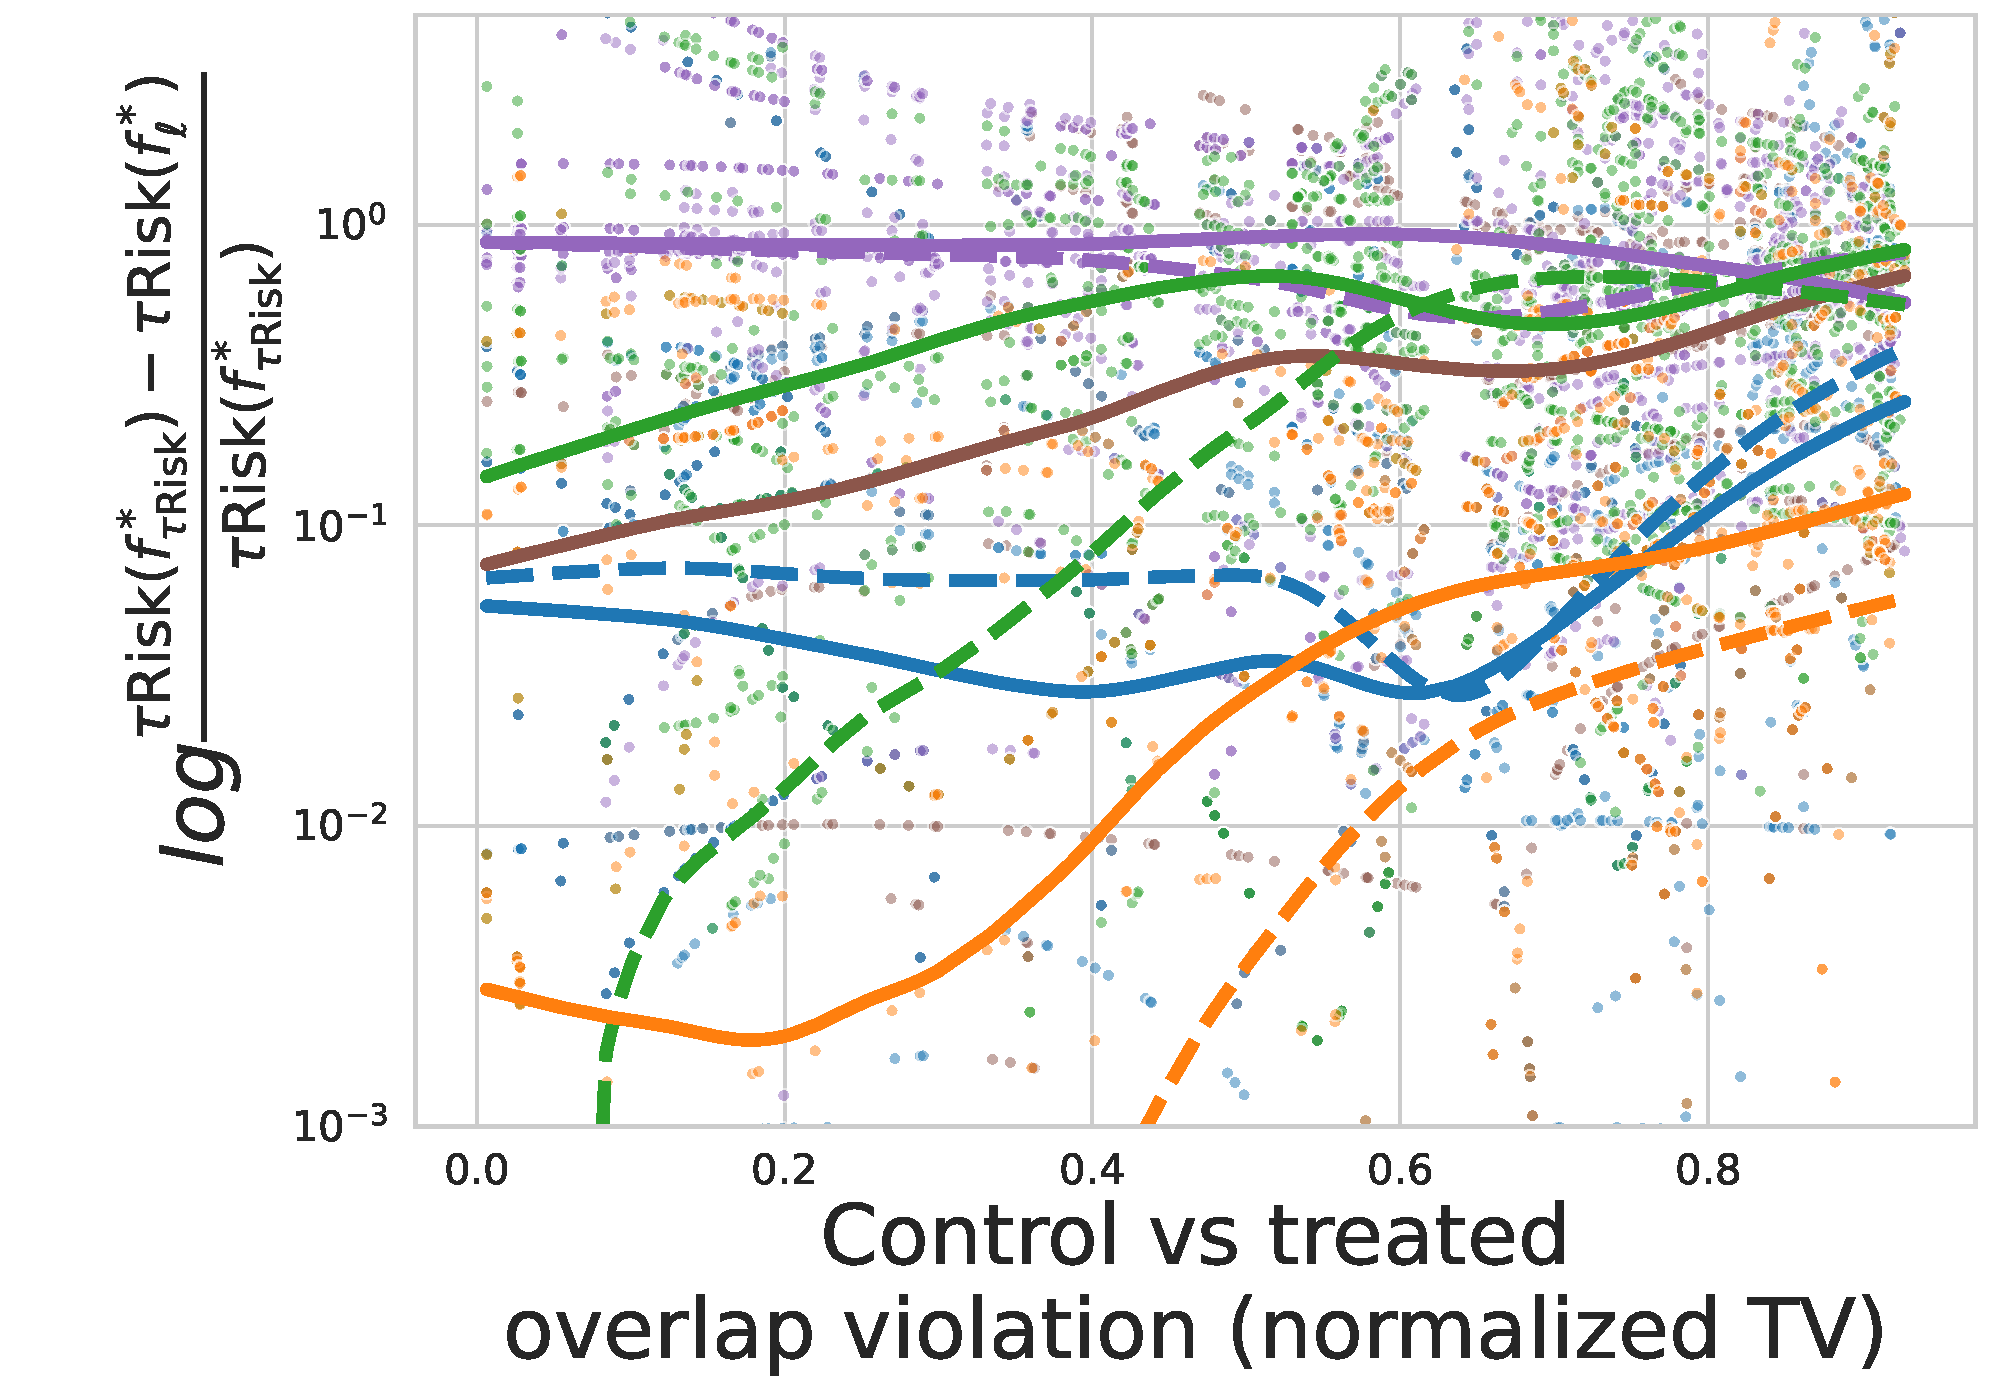
\includegraphics[width=\textwidth]{img/chapter_5/normalized_bias_tau_risk_to_best_method_caussim__nuisance_non_linear__candidates_ridge__overlap_01-247.pdf}
      \label{fig:normalized_bias_tau_risk_to_best_method_caussim}
    \end{subfigure}
    \hfill
    \begin{subfigure}[b]{0.44\textwidth}
      \centering
      \caption{\textbf{ACIC 2016}}
      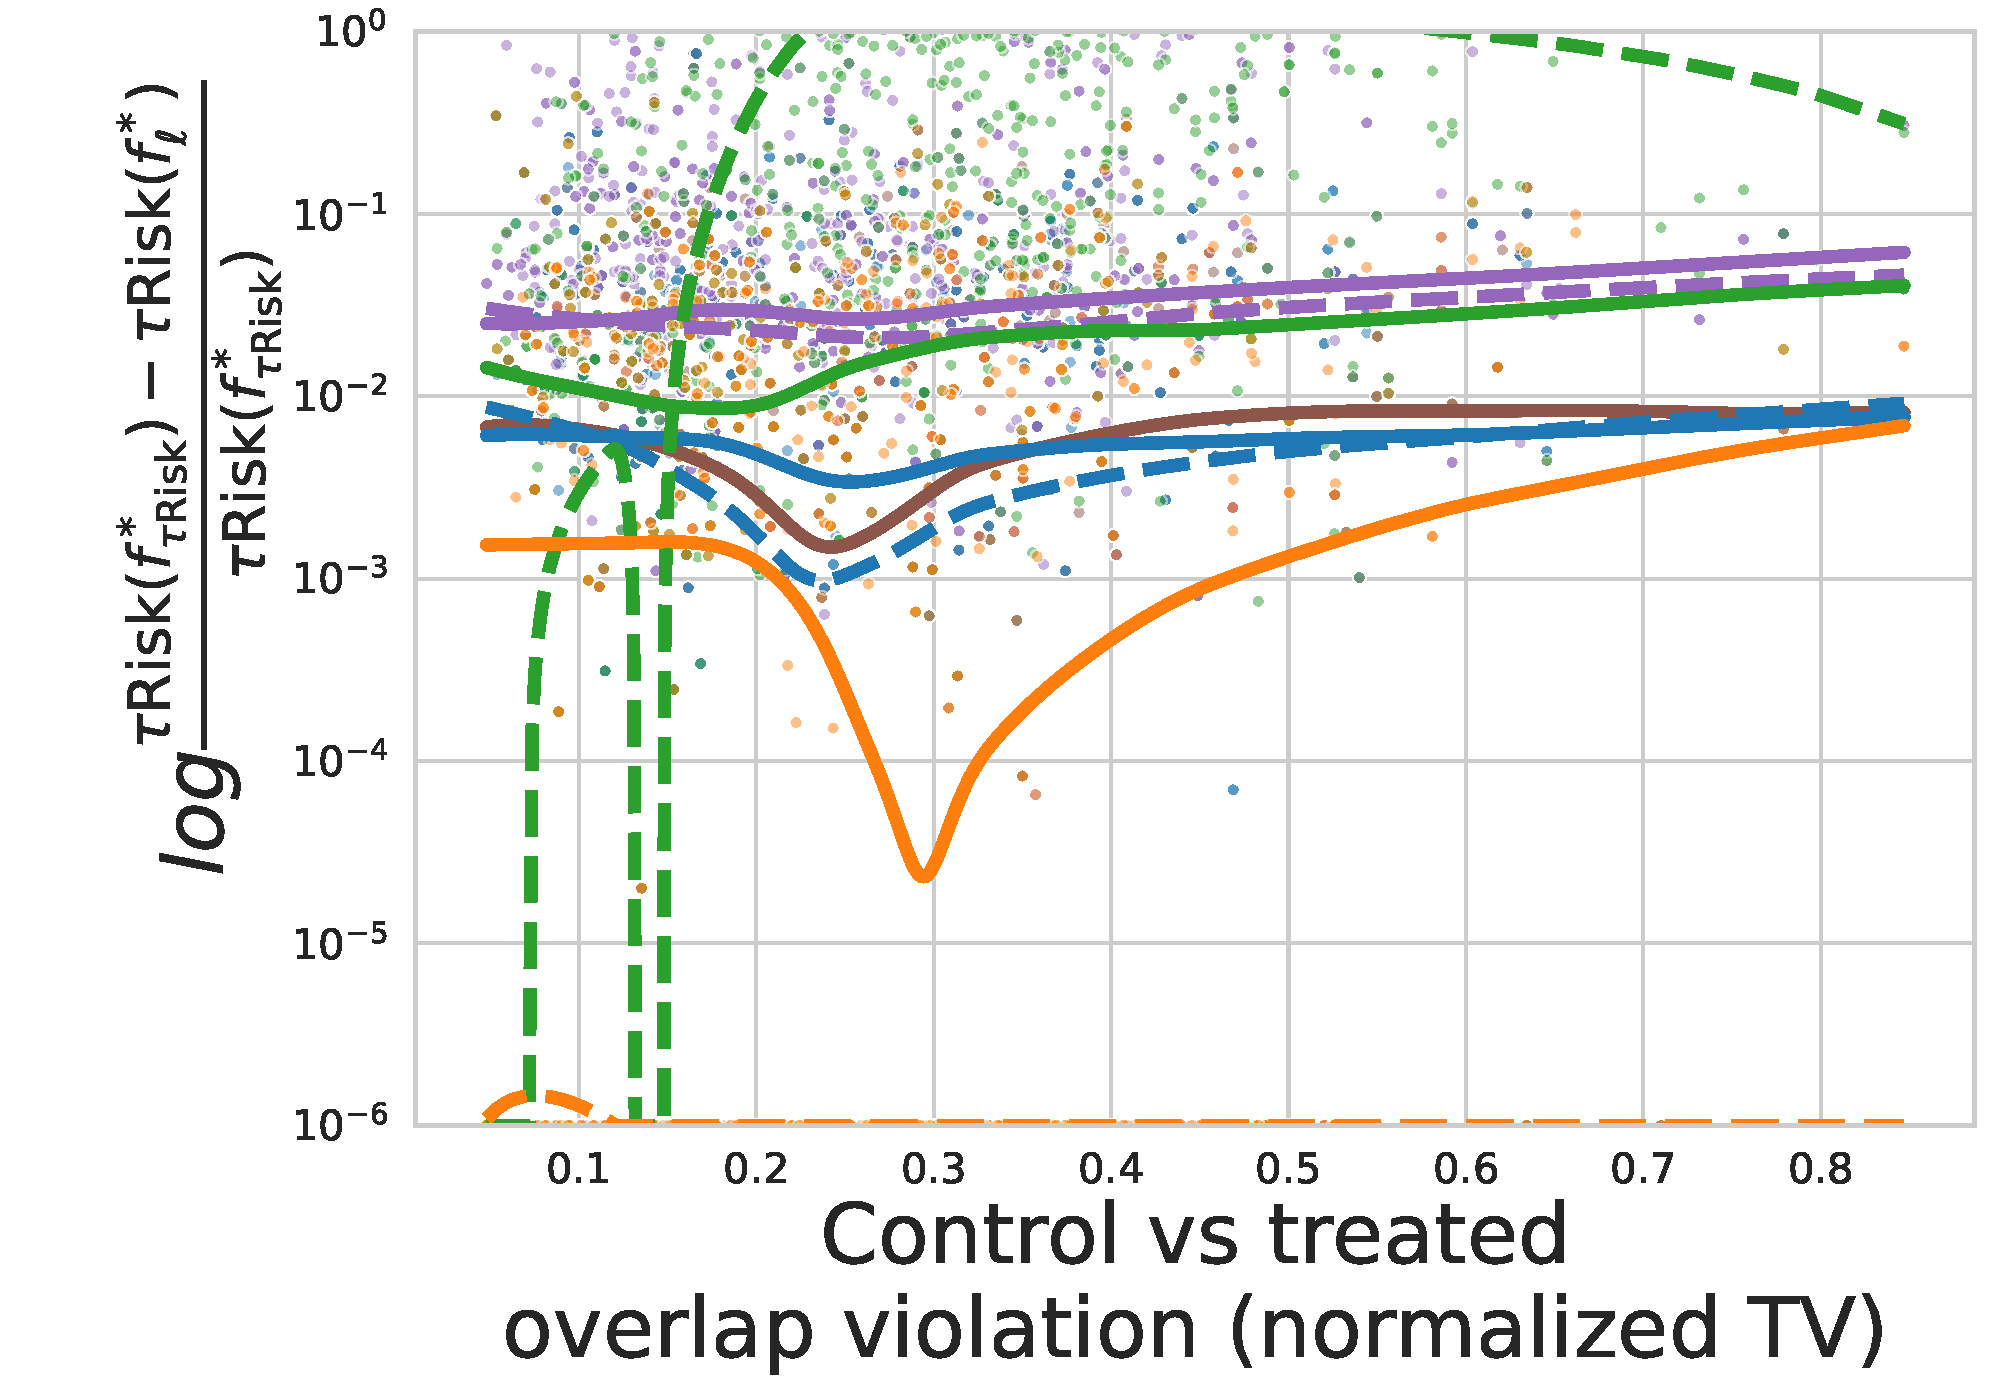
\includegraphics[width=\textwidth]{img/chapter_5/normalized_bias_tau_risk_to_best_method_acic_2016__nuisance_non_linear__candidates_hist_gradient_boosting__dgp_1-77__rs_1-10.pdf}
      \label{fig:normalized_bias_tau_risk_to_best_method_acic_2016}
    \end{subfigure}
    \hfill
    \begin{subfigure}[b]{0.10\textwidth}
      \centering
      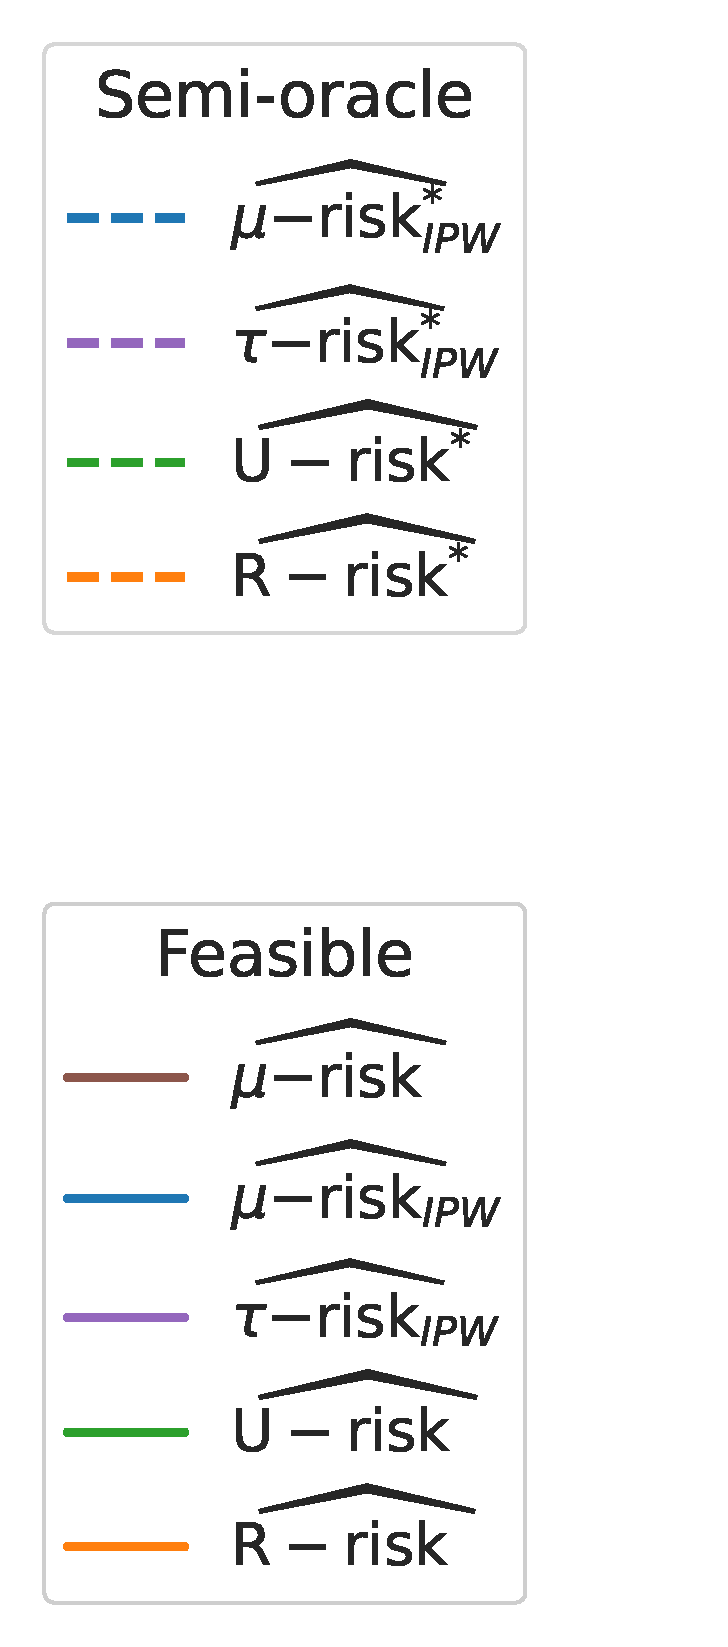
\includegraphics[width=1.5\textwidth]{img/chapter_5/legend_metrics.pdf}
    \end{subfigure}
    \begin{subfigure}[b]{0.44\textwidth}
      \centering
      \caption{\textbf{ACIC 2018}}
      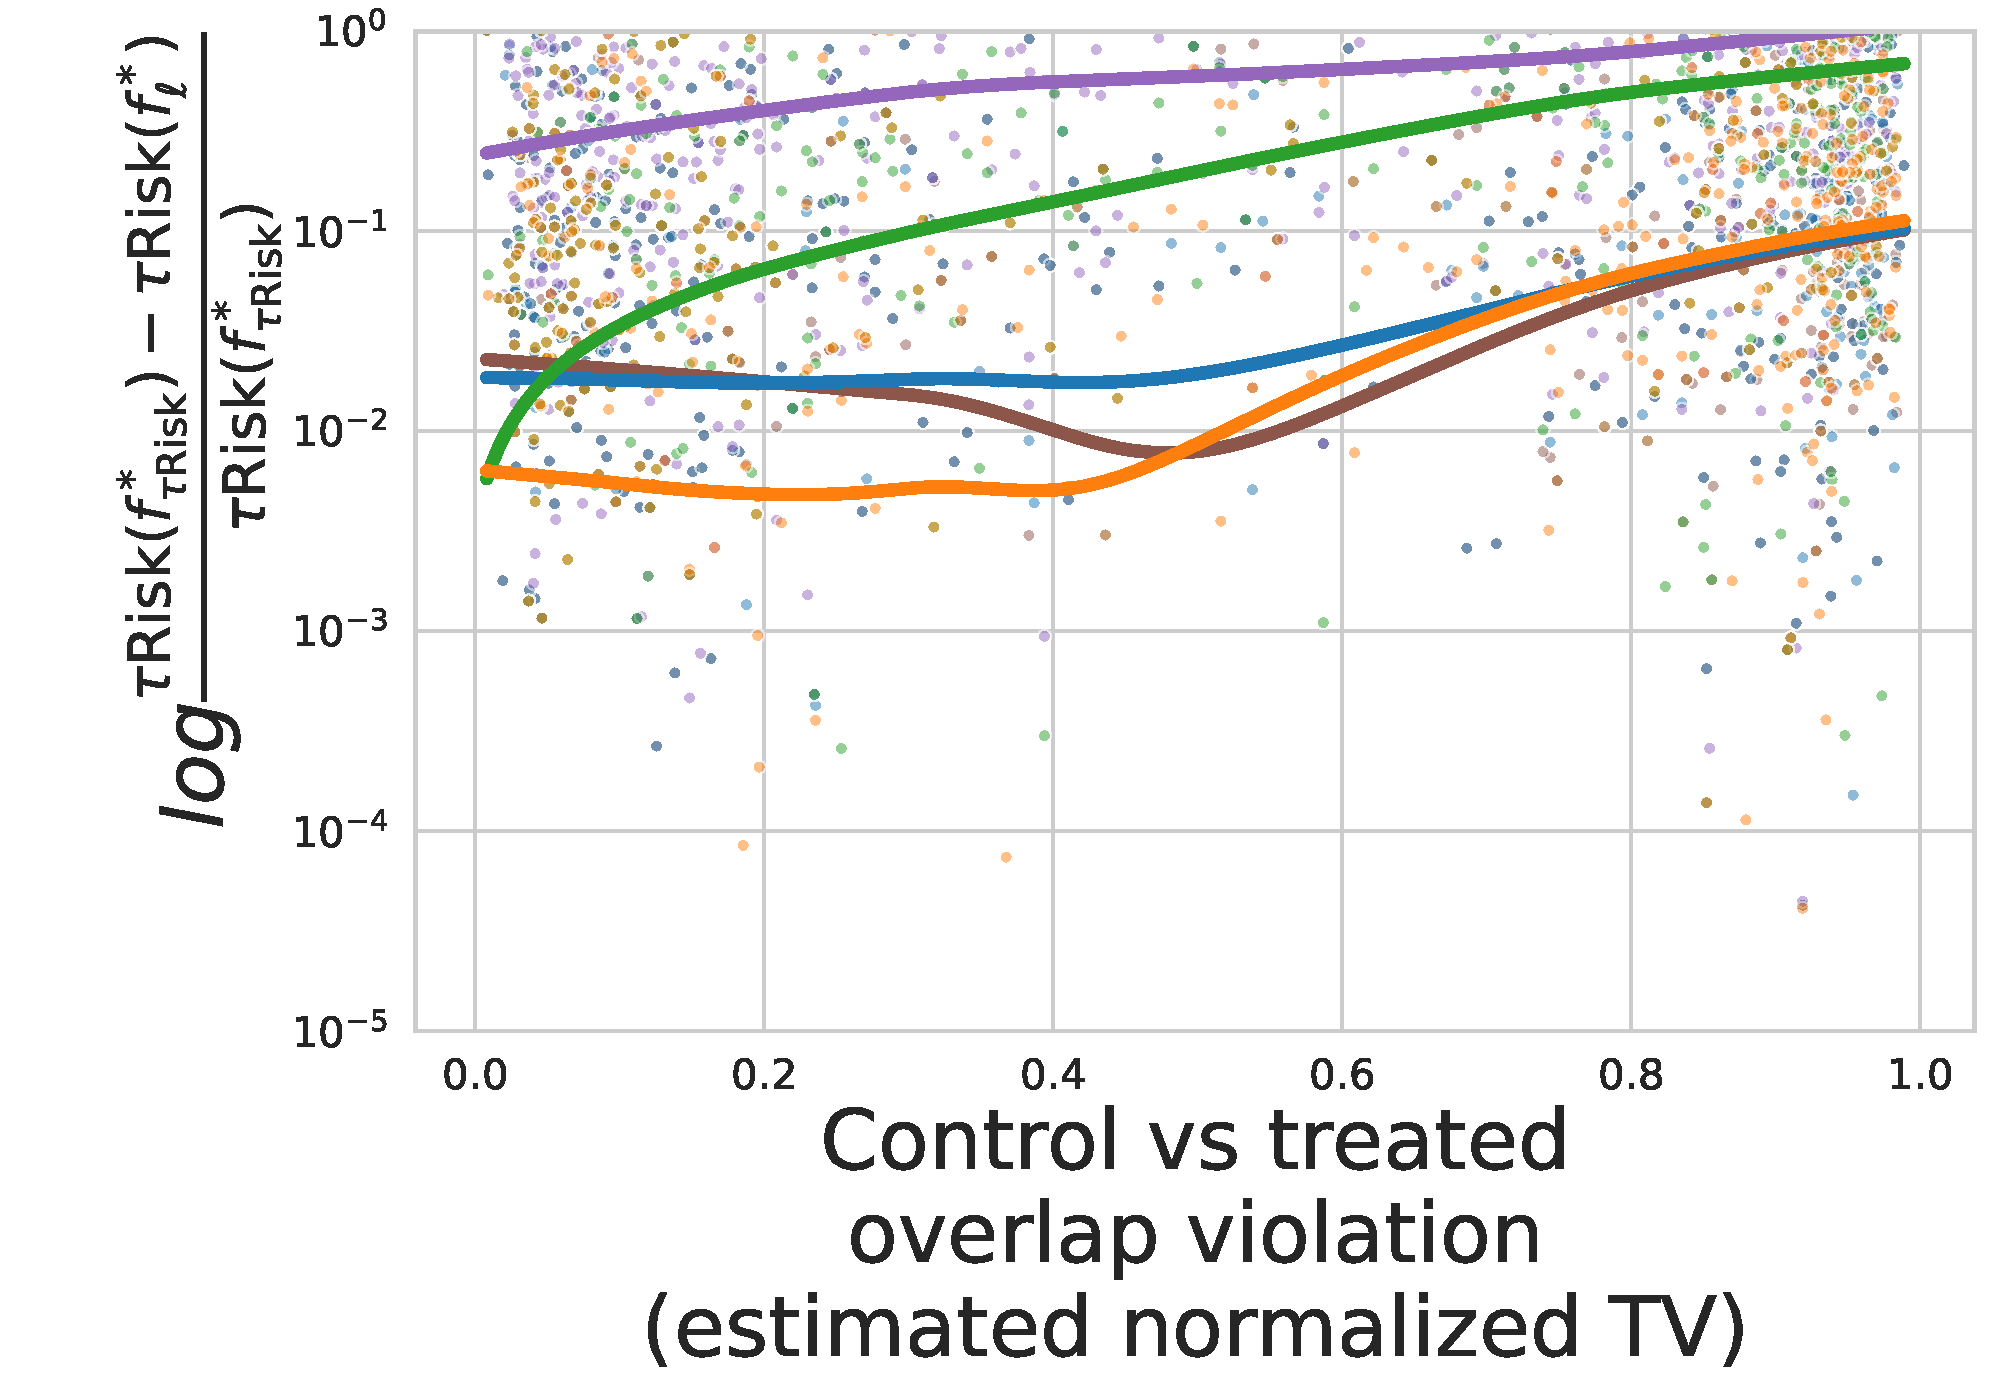
\includegraphics[width=\textwidth]{img/chapter_5/normalized_bias_tau_risk_to_best_method_acic_2018__nuisance_stacking__candidates_hist_gradient_boosting__tset_50.pdf}
      \label{fig:normalized_bias_tau_risk_to_best_method_acic_2018}
    \end{subfigure}
    \hfill
    \begin{subfigure}[b]{0.44\textwidth}
      \centering
      \caption{\textbf{TWINS}}
      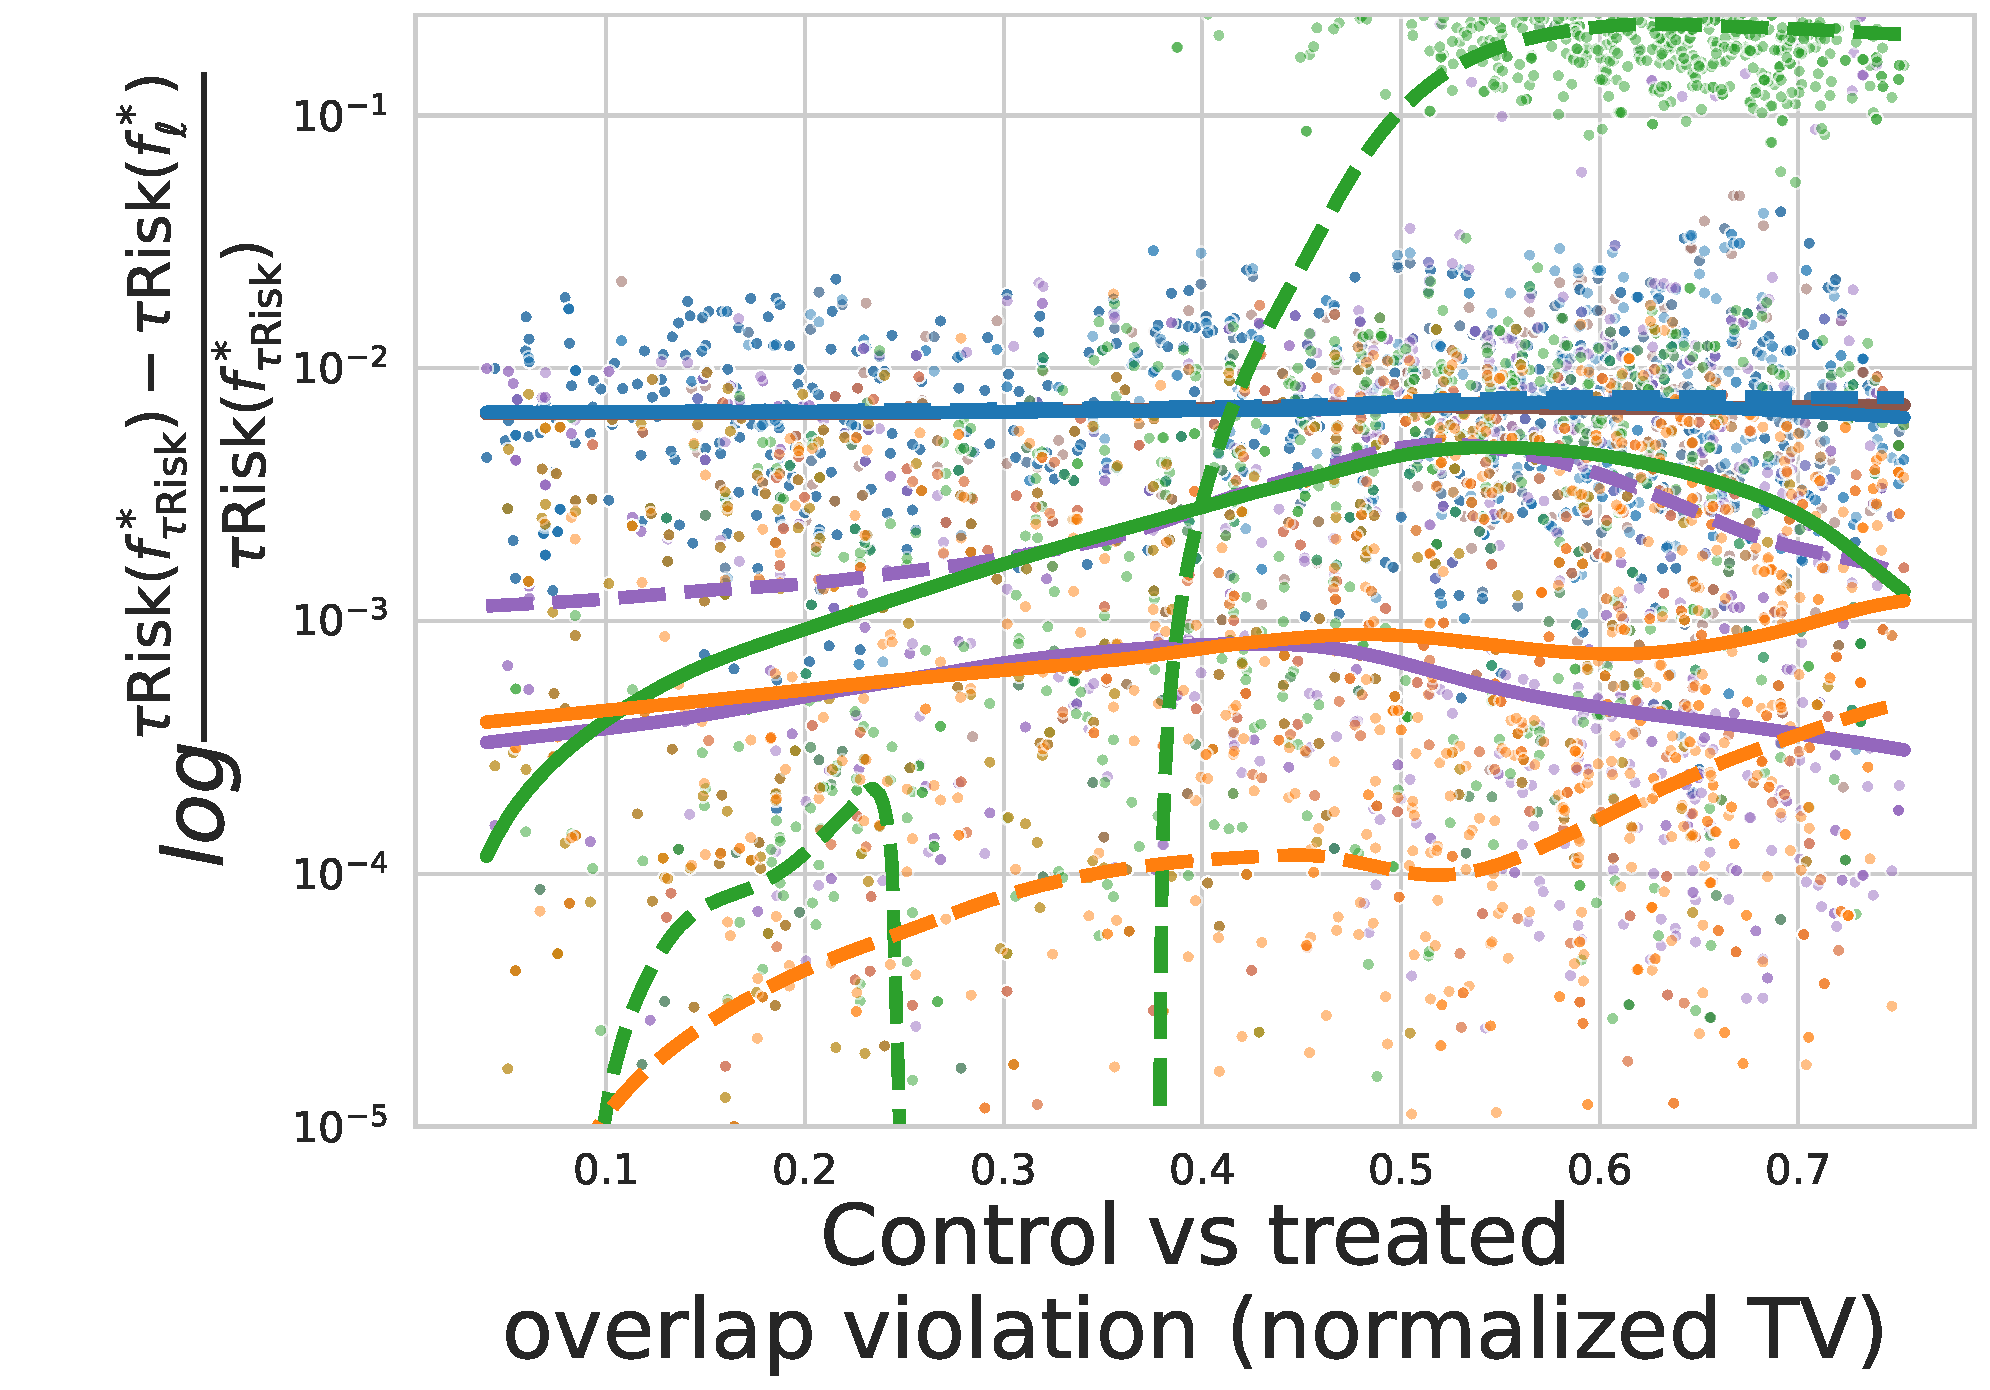
\includegraphics[width=\textwidth]{img/chapter_5/normalized_bias_tau_risk_to_best_method_twins__nuisance_stacking__candidates_hist_gradient_boosting__tset_50__overlap_11-296__rs_0-9_noise10.pdf}
      \label{fig:normalized_bias_tau_risk_to_best_method_twins}
    \end{subfigure}
    \hfill
    \begin{subfigure}[b]{0.10\textwidth}
      ~
    \end{subfigure}
    \caption{Metric performances by normalized tau-risk distance to the best
      method selected with $\tau\text{-risk}$. All nuisances are learned with the
      same estimator stacking gradient boosting and ridge regression. Doted and
      plain lines corresponds to 60\% lowess quantile estimates. This choice of
      quantile allows to see better the oracle metrics lines for which outliers with a value
      of 0 distord the curves.}
    \label
    {apd:all_datasets_normalized_bias_tau_risk_to_best_method}
  \end{figure}



  \paragraph{Figure \ref{apd:fig:procedures_comparison_all_metrics} - Stacked models for the nuisances is more efficient}
  For each metrics the benefit of
  using a stacked model of linear and boosting estimators for nuisances compared
  to a linear model. The evaluation measure is Kendall's tau relative to the
  oracle $R\text{-risk}^{\star}$ to have a stable reference between exepriments.
  Thus, we do not include in this analysis the ACIC 2018 dataset since
  $R\text{-risk}^{\star}$ is not available due to the lack of the true propensity
  score.

  \begin{figure}
    \begin{subfigure}[b]{0.9\textwidth}
      %\centering
      \caption{\textbf{Caussim}}
      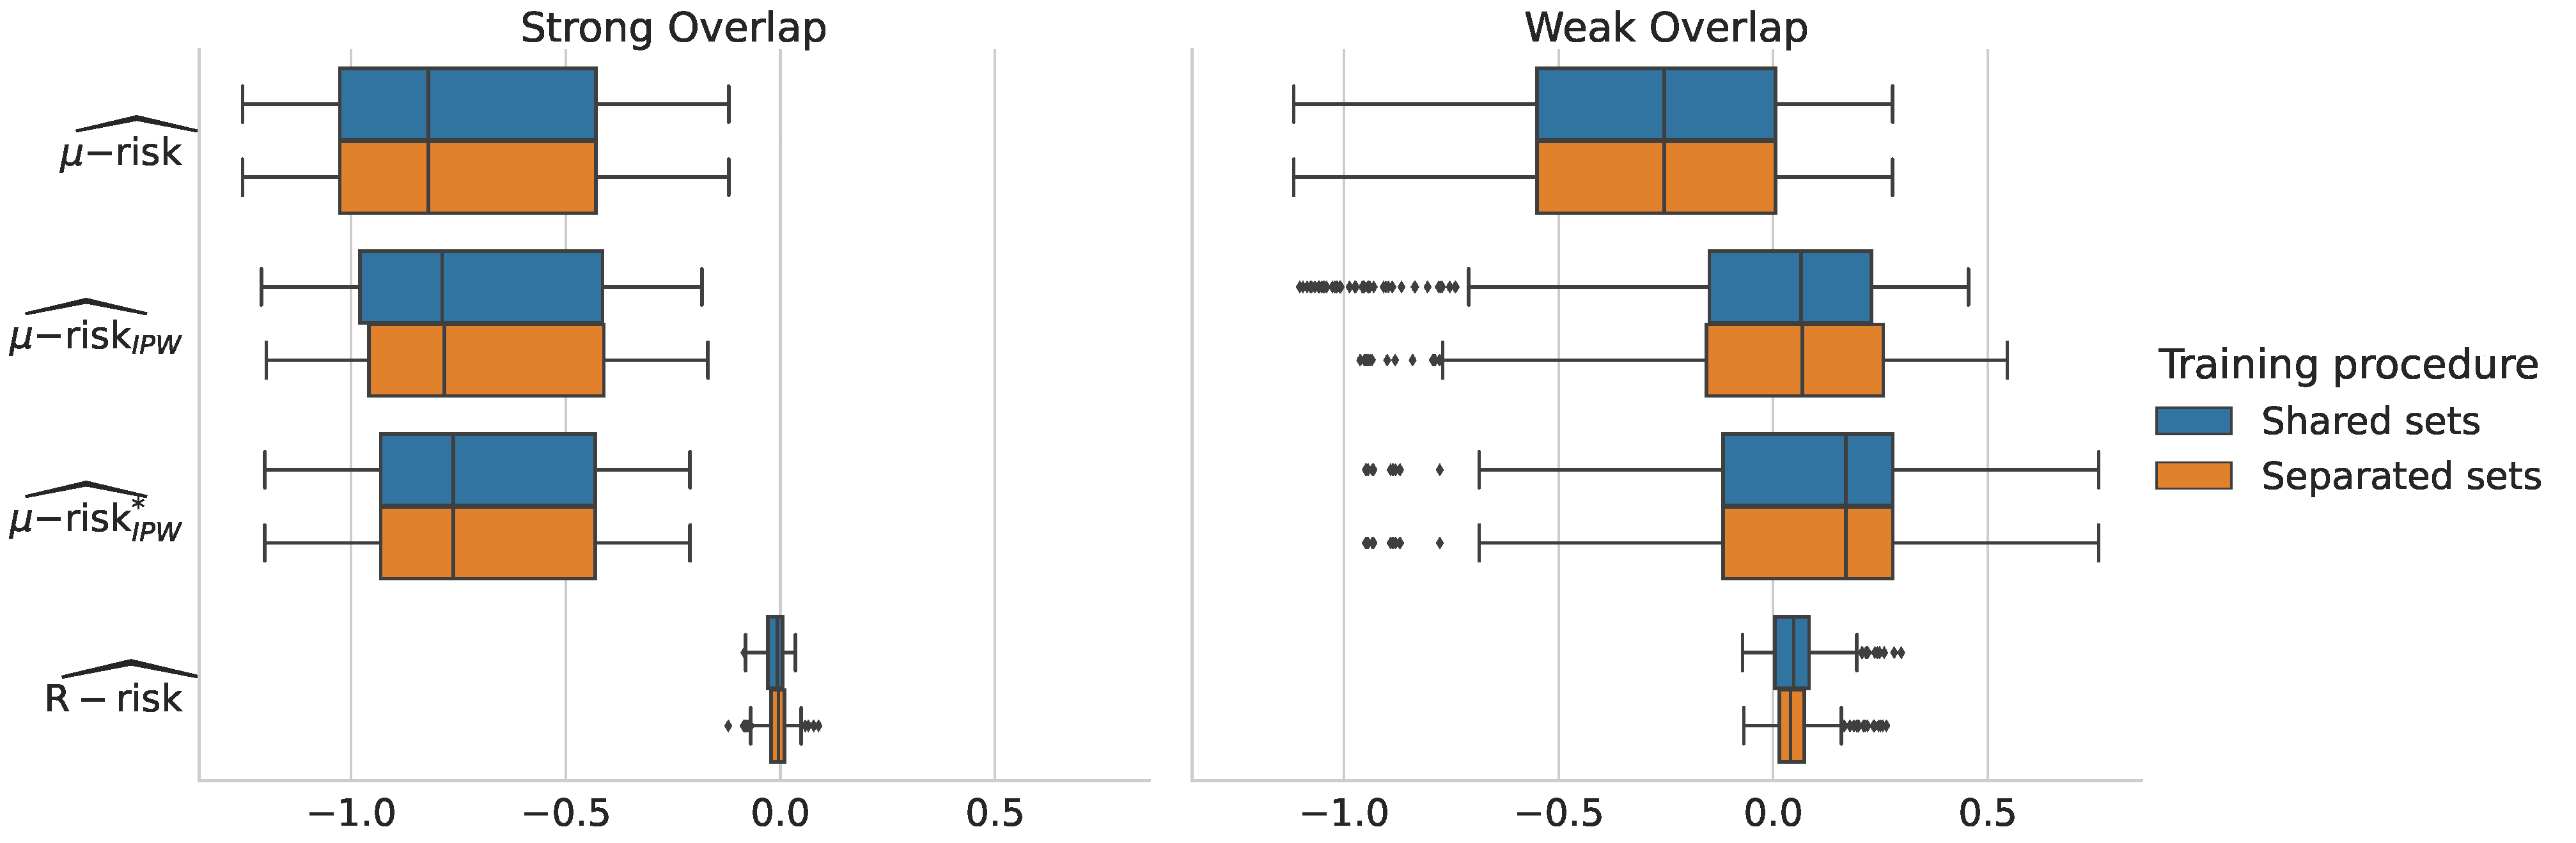
\includegraphics[width=1.15\textwidth]{img/chapter_5/_3_procedure_Caussim_N5000__ref_metric_oracle_r_risk_training_procedure.pdf}
      \label{fig:experiments:procedures_comparison:caussim}
    \end{subfigure}
    \hfill
    \begin{subfigure}[b]{0.9\textwidth}
      \centering
      \caption{\textbf{ACIC 2016}}
      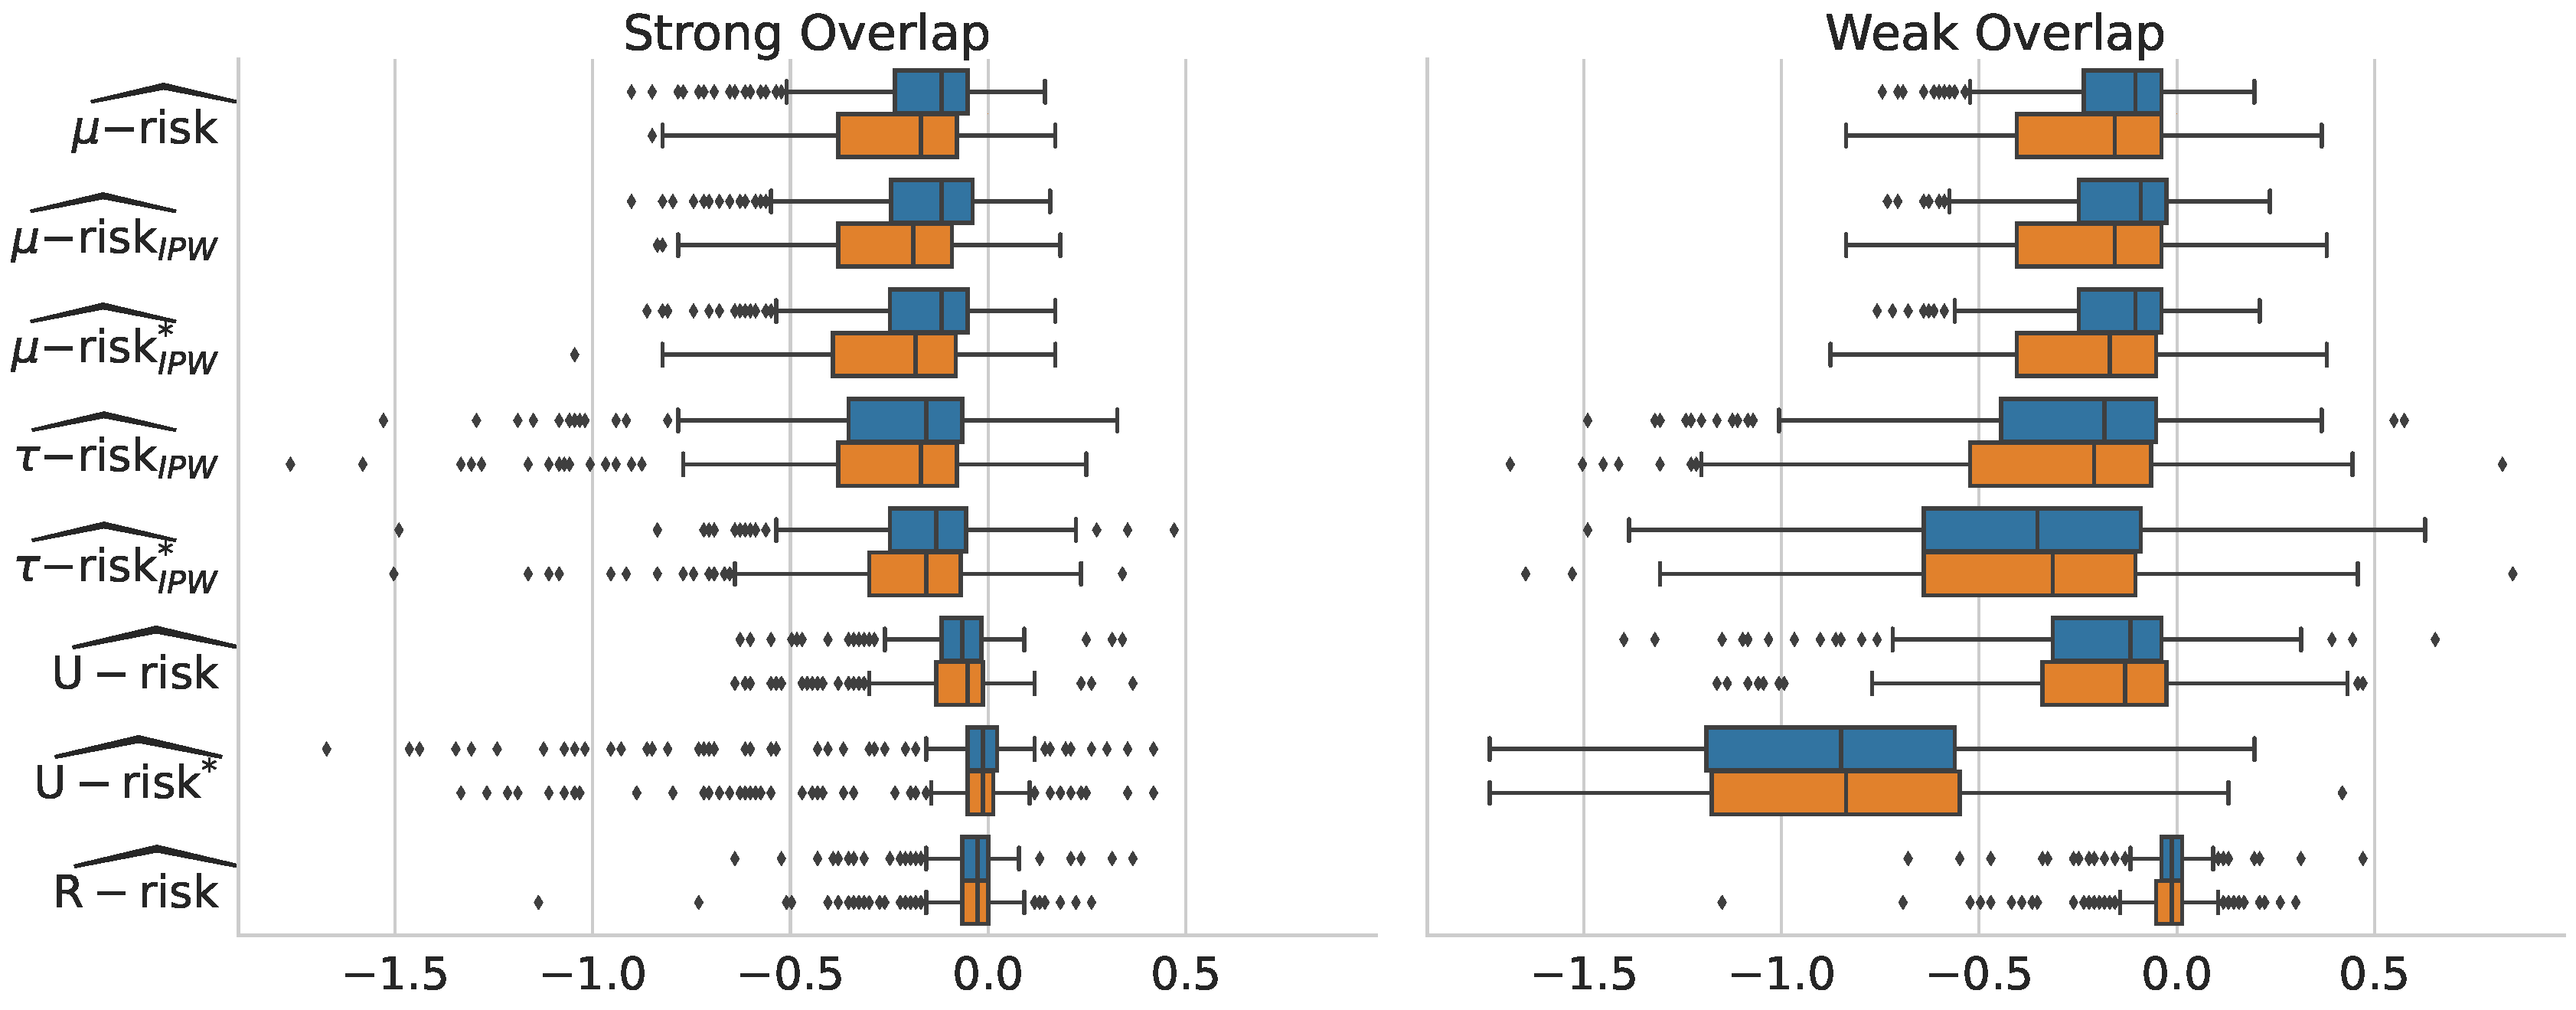
\includegraphics[width=1\textwidth]{img/chapter_5/_3_procedure_ACIC2016_N4802__ref_metric_oracle_r_risk_training_procedure.pdf}
      \label{fig:experiments:procedures_comparison:acic_2016}
    \end{subfigure}
    \hfill
    \begin{subfigure}[b]{0.9\textwidth}
      \centering
      \caption{\textbf{Twins}}
      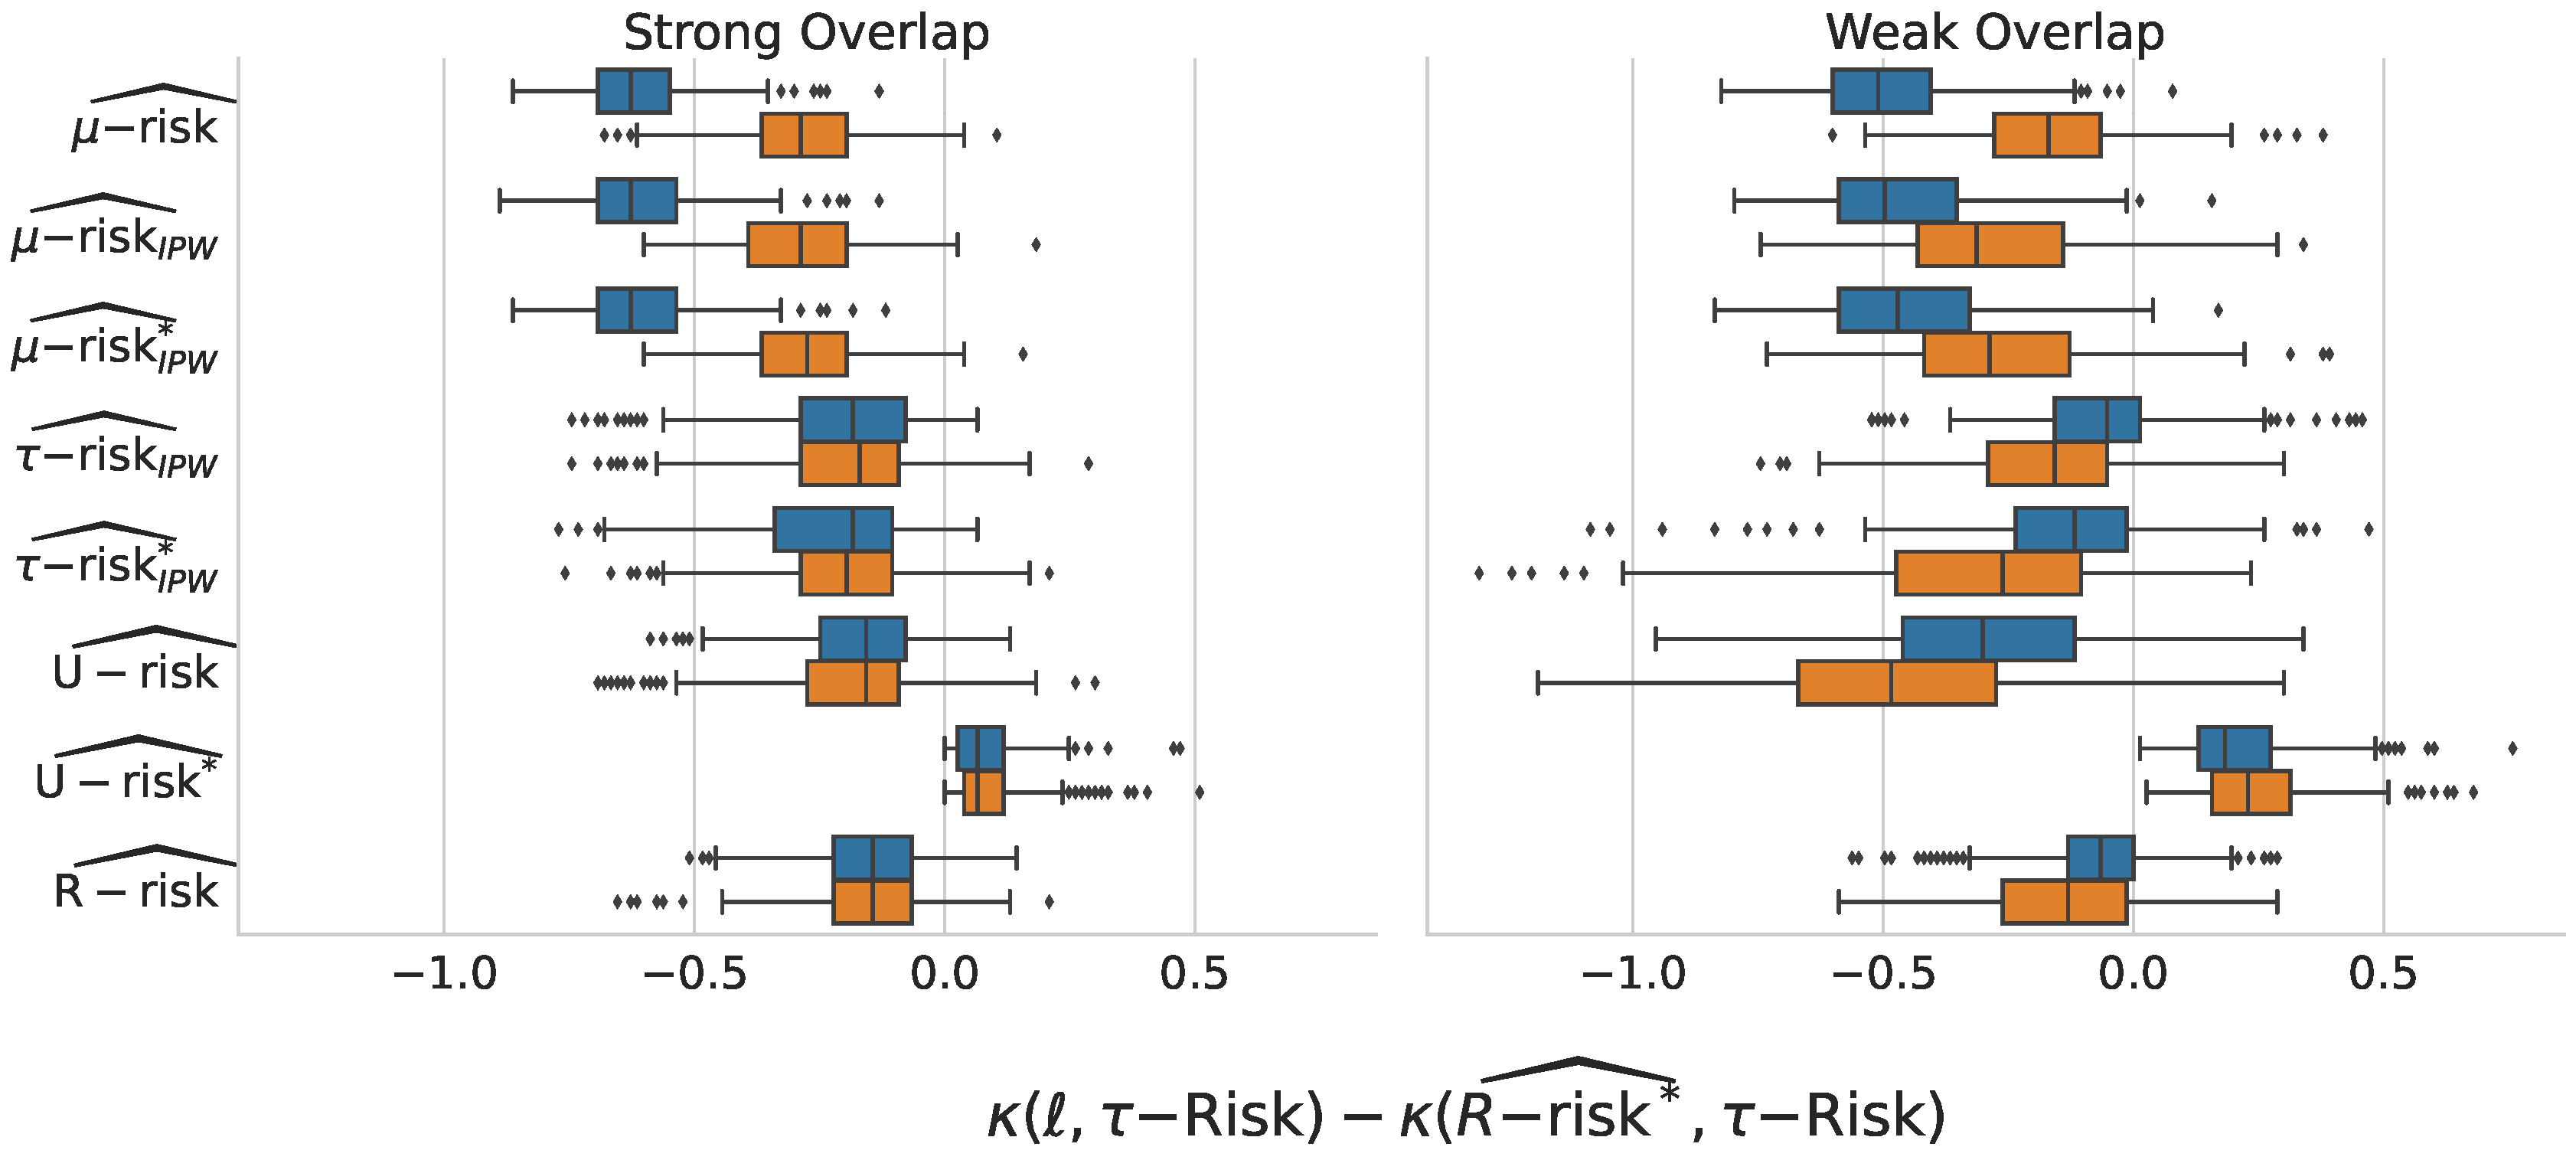
\includegraphics[width=1\textwidth]{img/chapter_5/_3_procedure_Twins_N11984__ref_metric_oracle_r_risk_training_procedure.pdf}
      \label{fig:experiments:procedures_comparison:twins}
    \end{subfigure}
    \hfill
    \caption{Results are similar between the \textcolor{MidnightBlue}{Shared
        nuisances/candidate set} and
      the \textcolor{RedOrange}{Separated nuisances set} procedure. The
      experience has not been run on the full metrics for Caussim due to computation costs.}\label
    {apd:fig:procedures_comparison_all_metrics}
  \end{figure}

  \paragraph{Figure \ref{apd:fig:all_datasets_overlap_effect} Low population
    overlap hinders model selection for all metrics}



  \begin{figure}
    \centering
    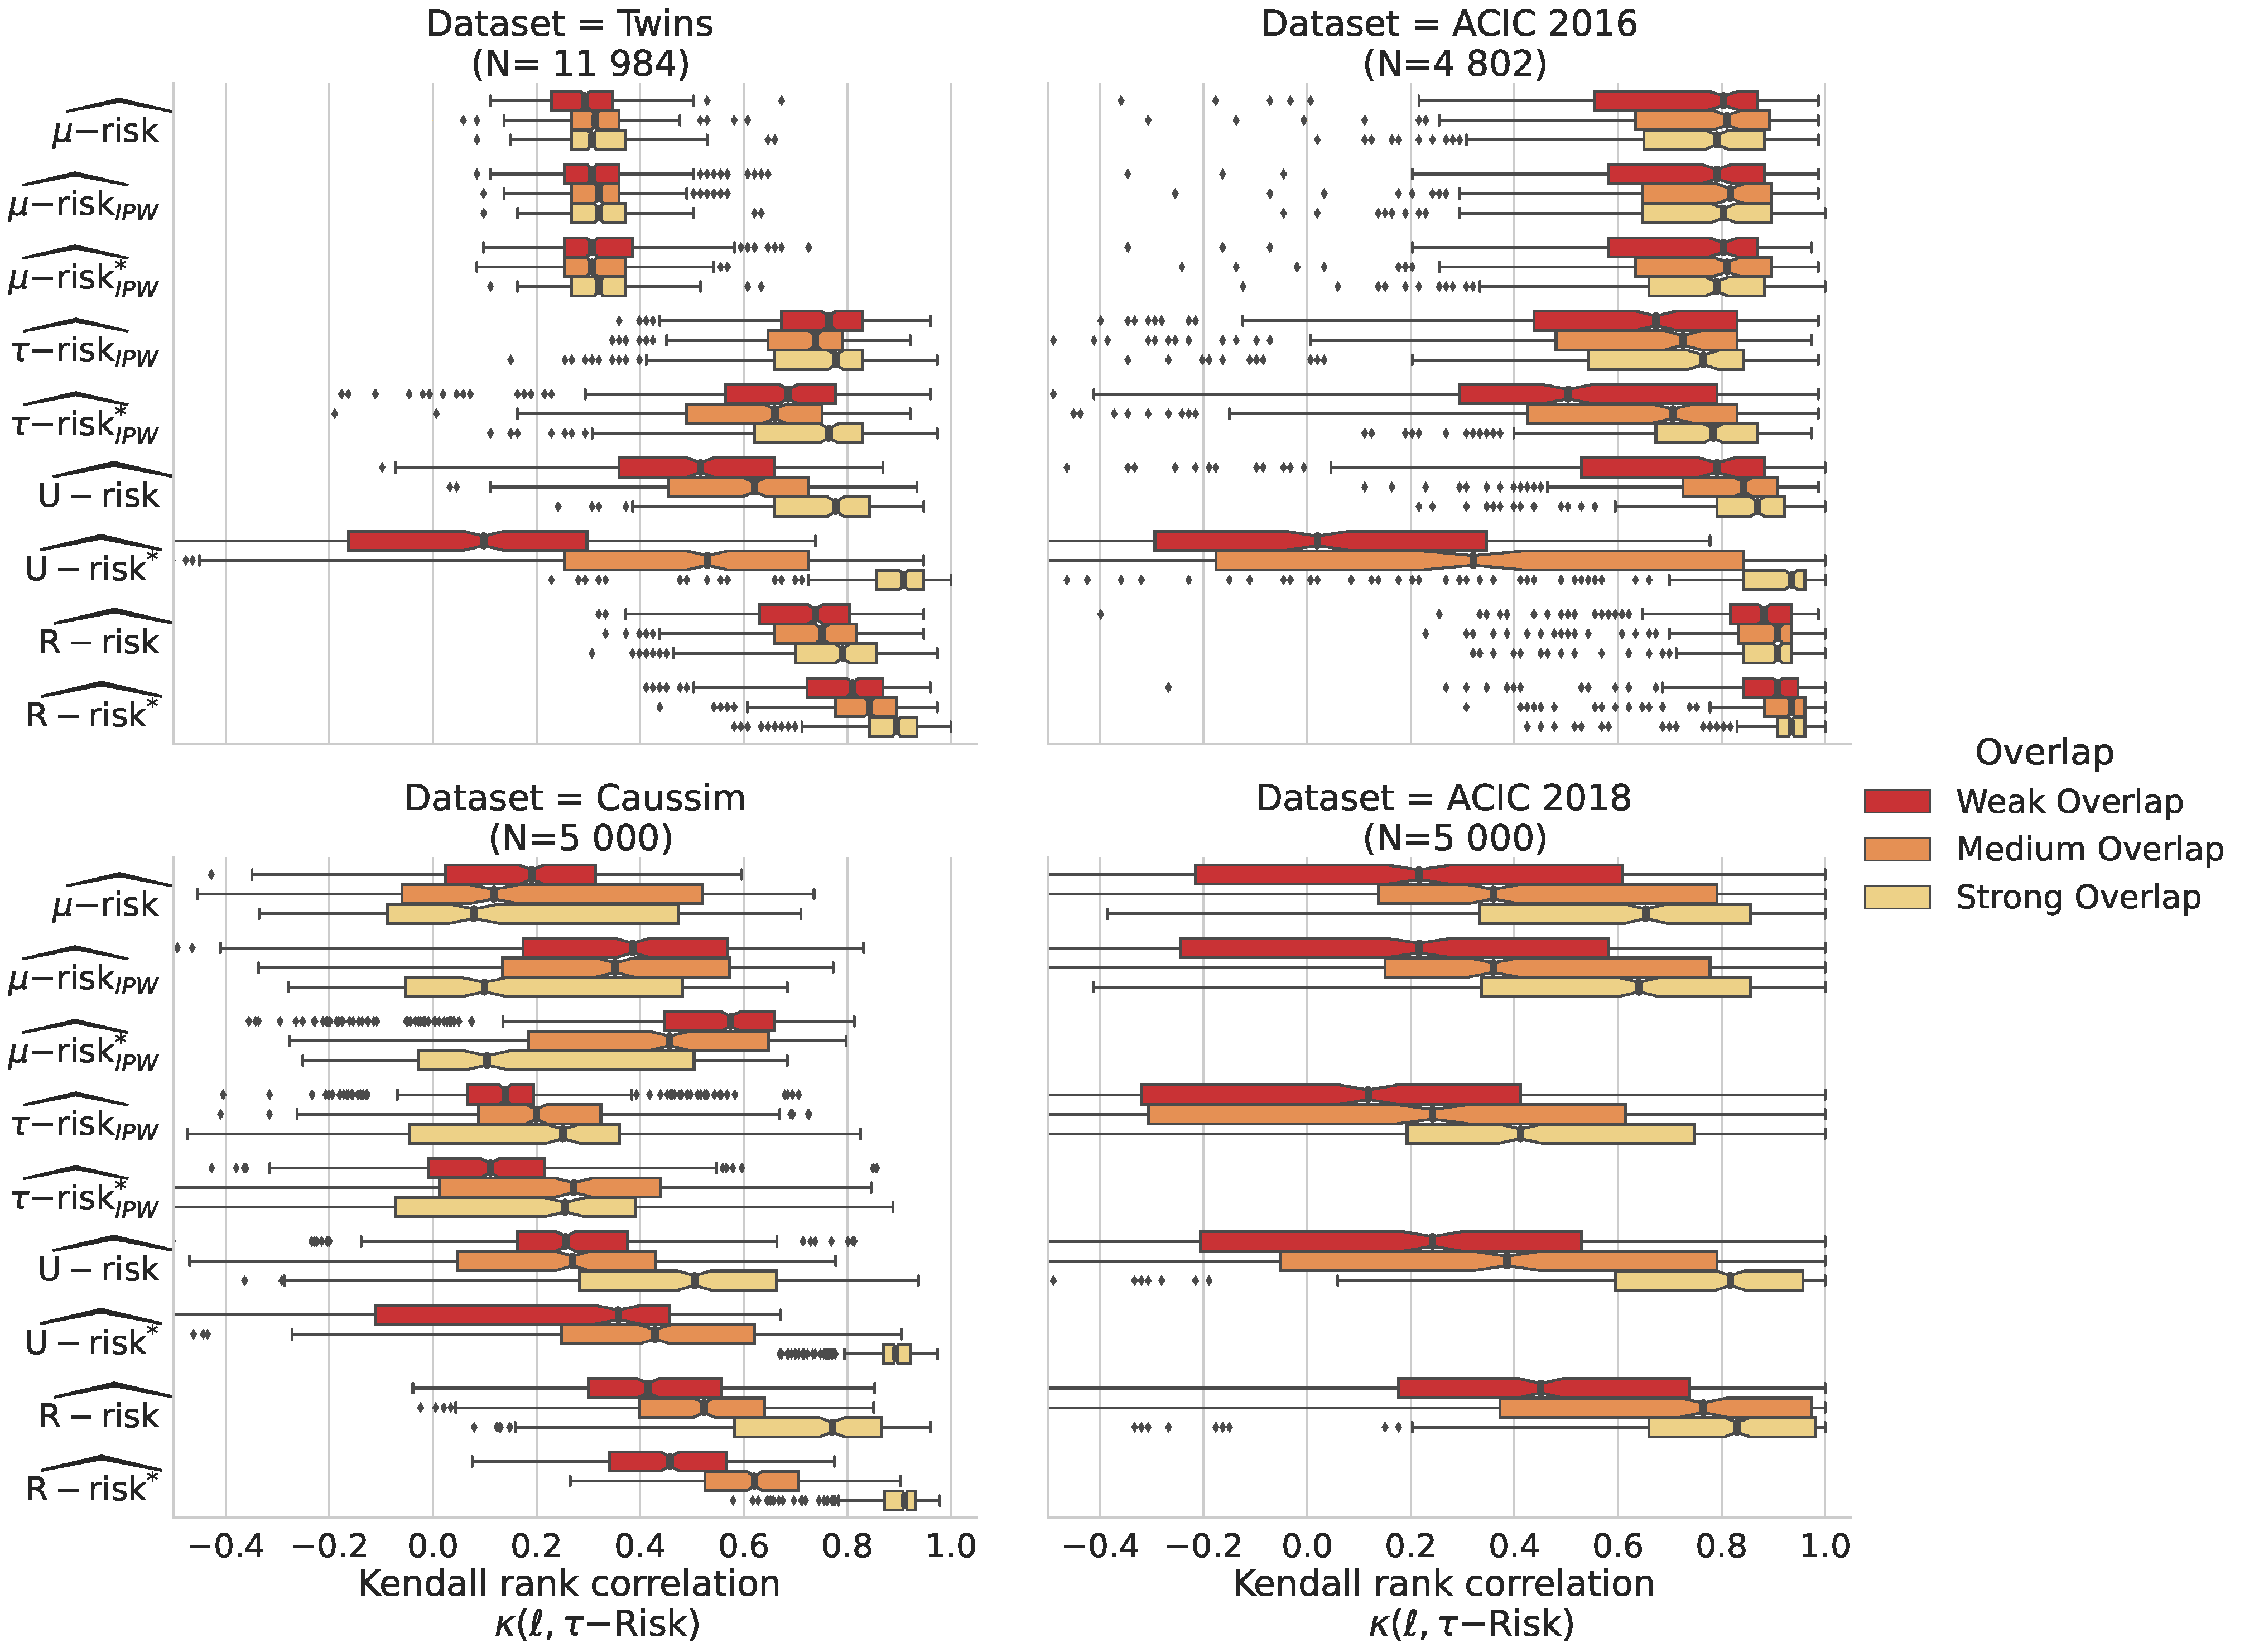
\includegraphics[width=\textwidth]{img/chapter_5/_2_overlap_influence_overlap_by_bin_comparaison_kendall_by_Dataset.pdf}
    \hfill
    \caption{\textbf{Low population overlap hinders causal model selection for all
        metrics}:
      Kendall's $\tau$ agreement with $\tau\text{-risk}$. Strong, medium and weak overlap
      correspond
      to the tertiles of the overlap distribution measured with Normalized Total
      Varation eq. \ref{eq:ntv}.}\label{apd:fig:all_datasets_overlap_effect}
  \end{figure}


  \paragraph{Figure \ref{apd:fig:nuisances_comparison} - Stacked models for the nuisances is more efficient}
  For each metrics the benefit of
  using a stacked model of linear and boosting estimators for nuisances compared
  to a linear model. The evaluation measure is Kendall's tau relative to the
  oracle $R\text{-risk}^{\star}$ to have a stable reference between exepriments.
  Thus, we do not include in this analysis the ACIC 2018 dataset since
  $R\text{-risk}^{\star}$ is not available due to the lack of the true propensity
  score.

  \begin{figure}
    \begin{subfigure}[b]{0.49\textwidth}
      \centering
      \caption{\textbf{Twins}}
      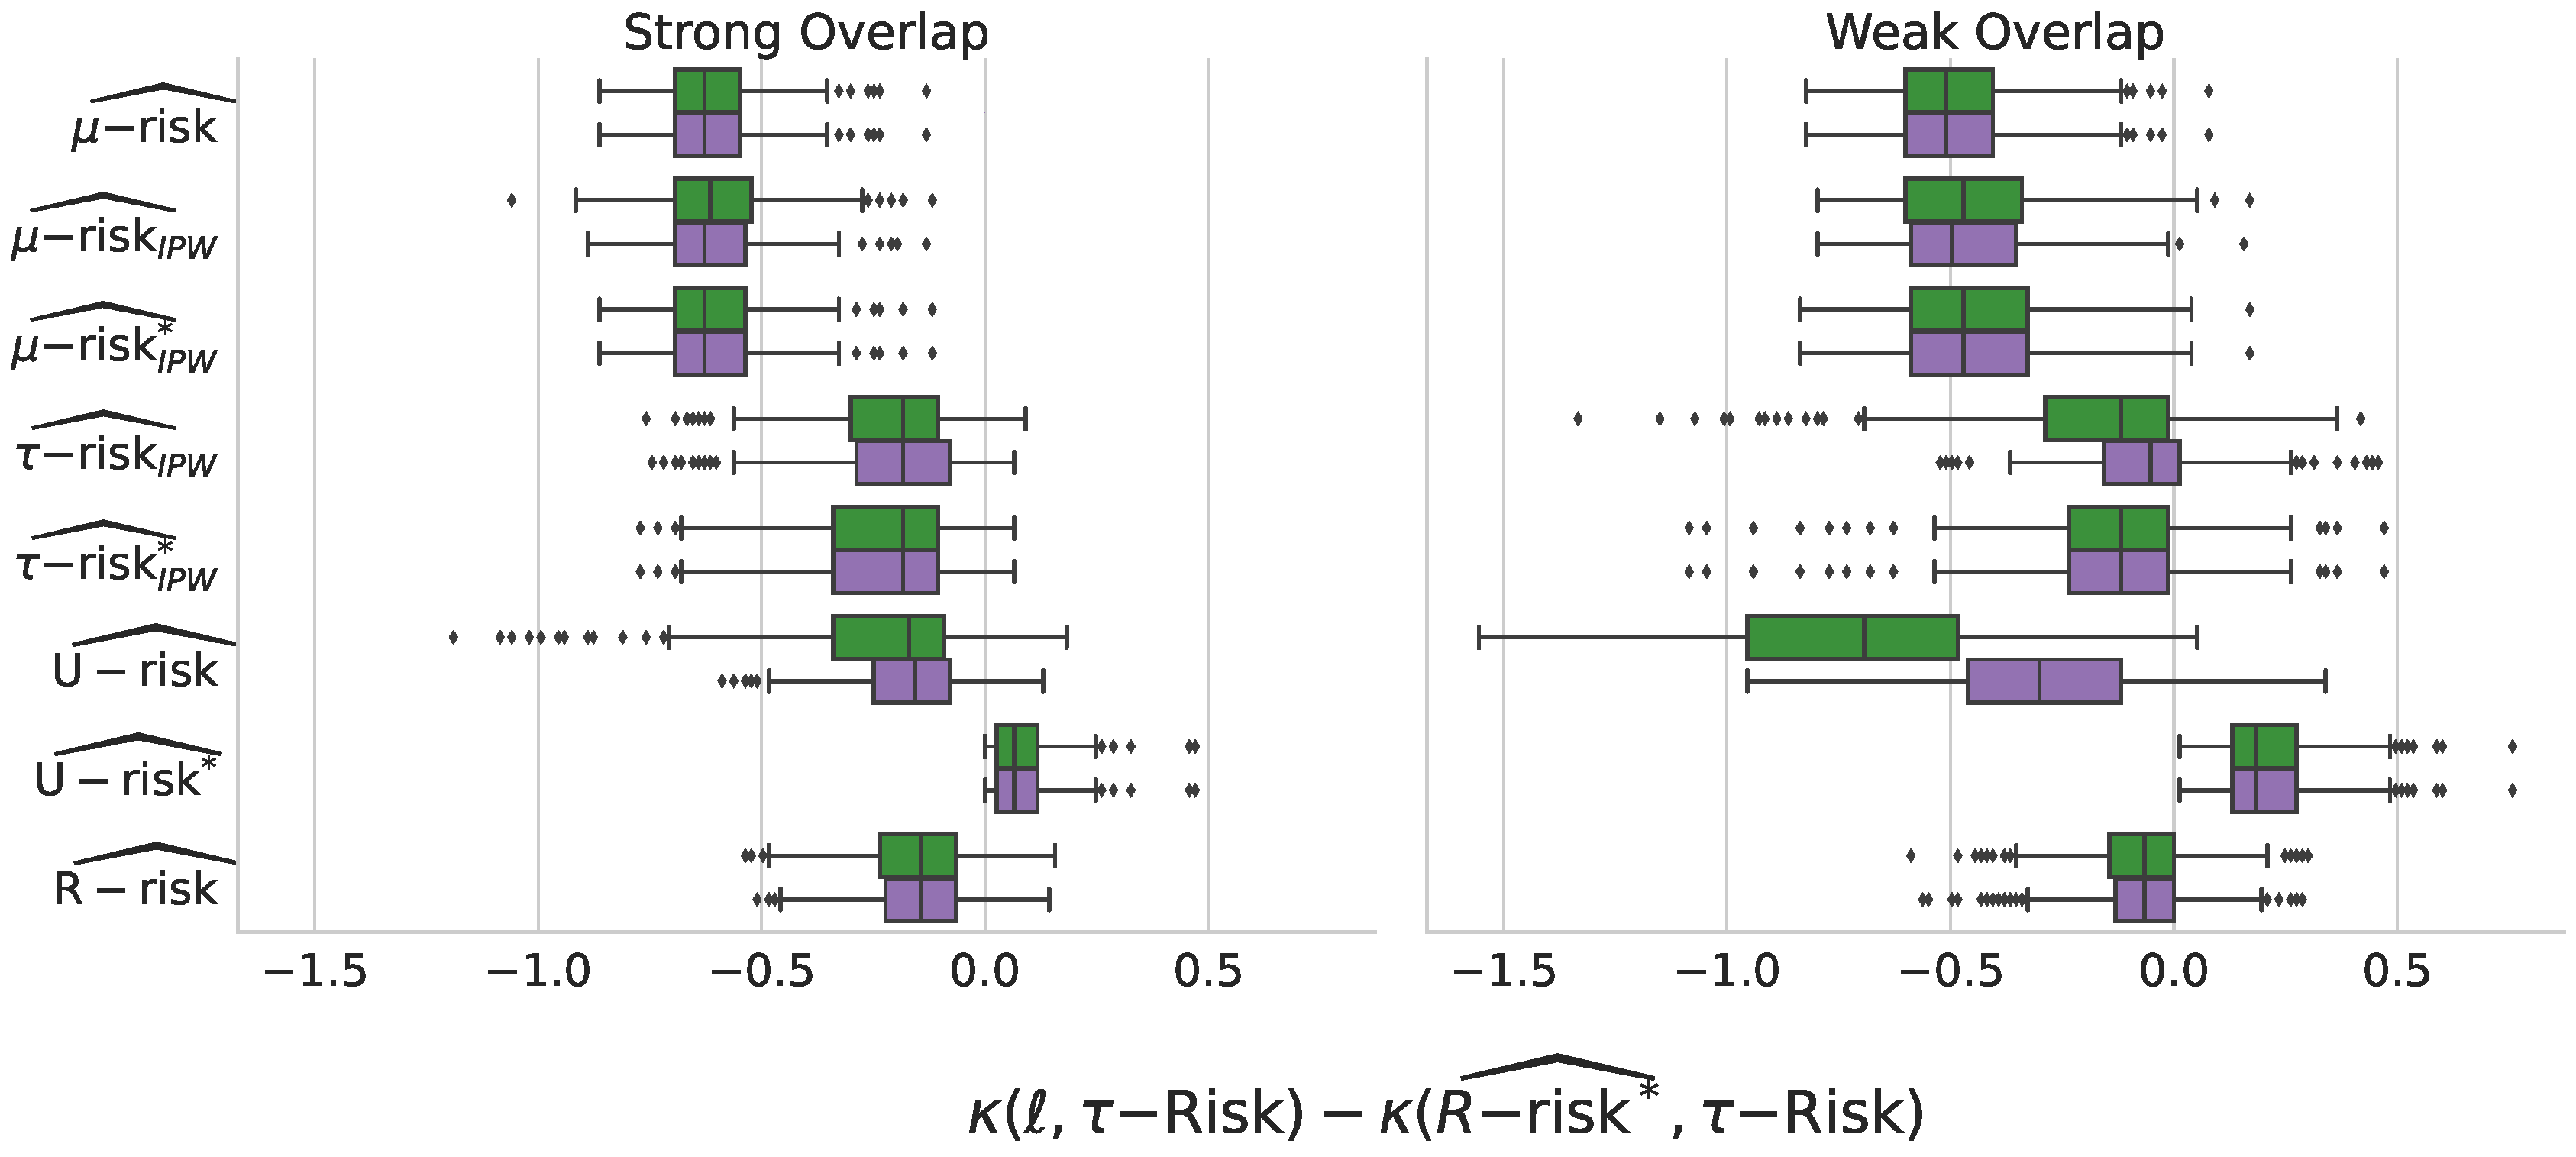
\includegraphics[width=1\textwidth]{img/chapter_5/_4_nuisance_models_Twins_N11984__ref_metric_oracle_r_risk_nuisance_models.pdf}
      \label{fig:experiments:nuisance_comparison:twins}
    \end{subfigure}
    \hfill
    \begin{subfigure}[b]{0.49\textwidth}
      \centering
      \caption{\textbf{Twins downsampled}}
      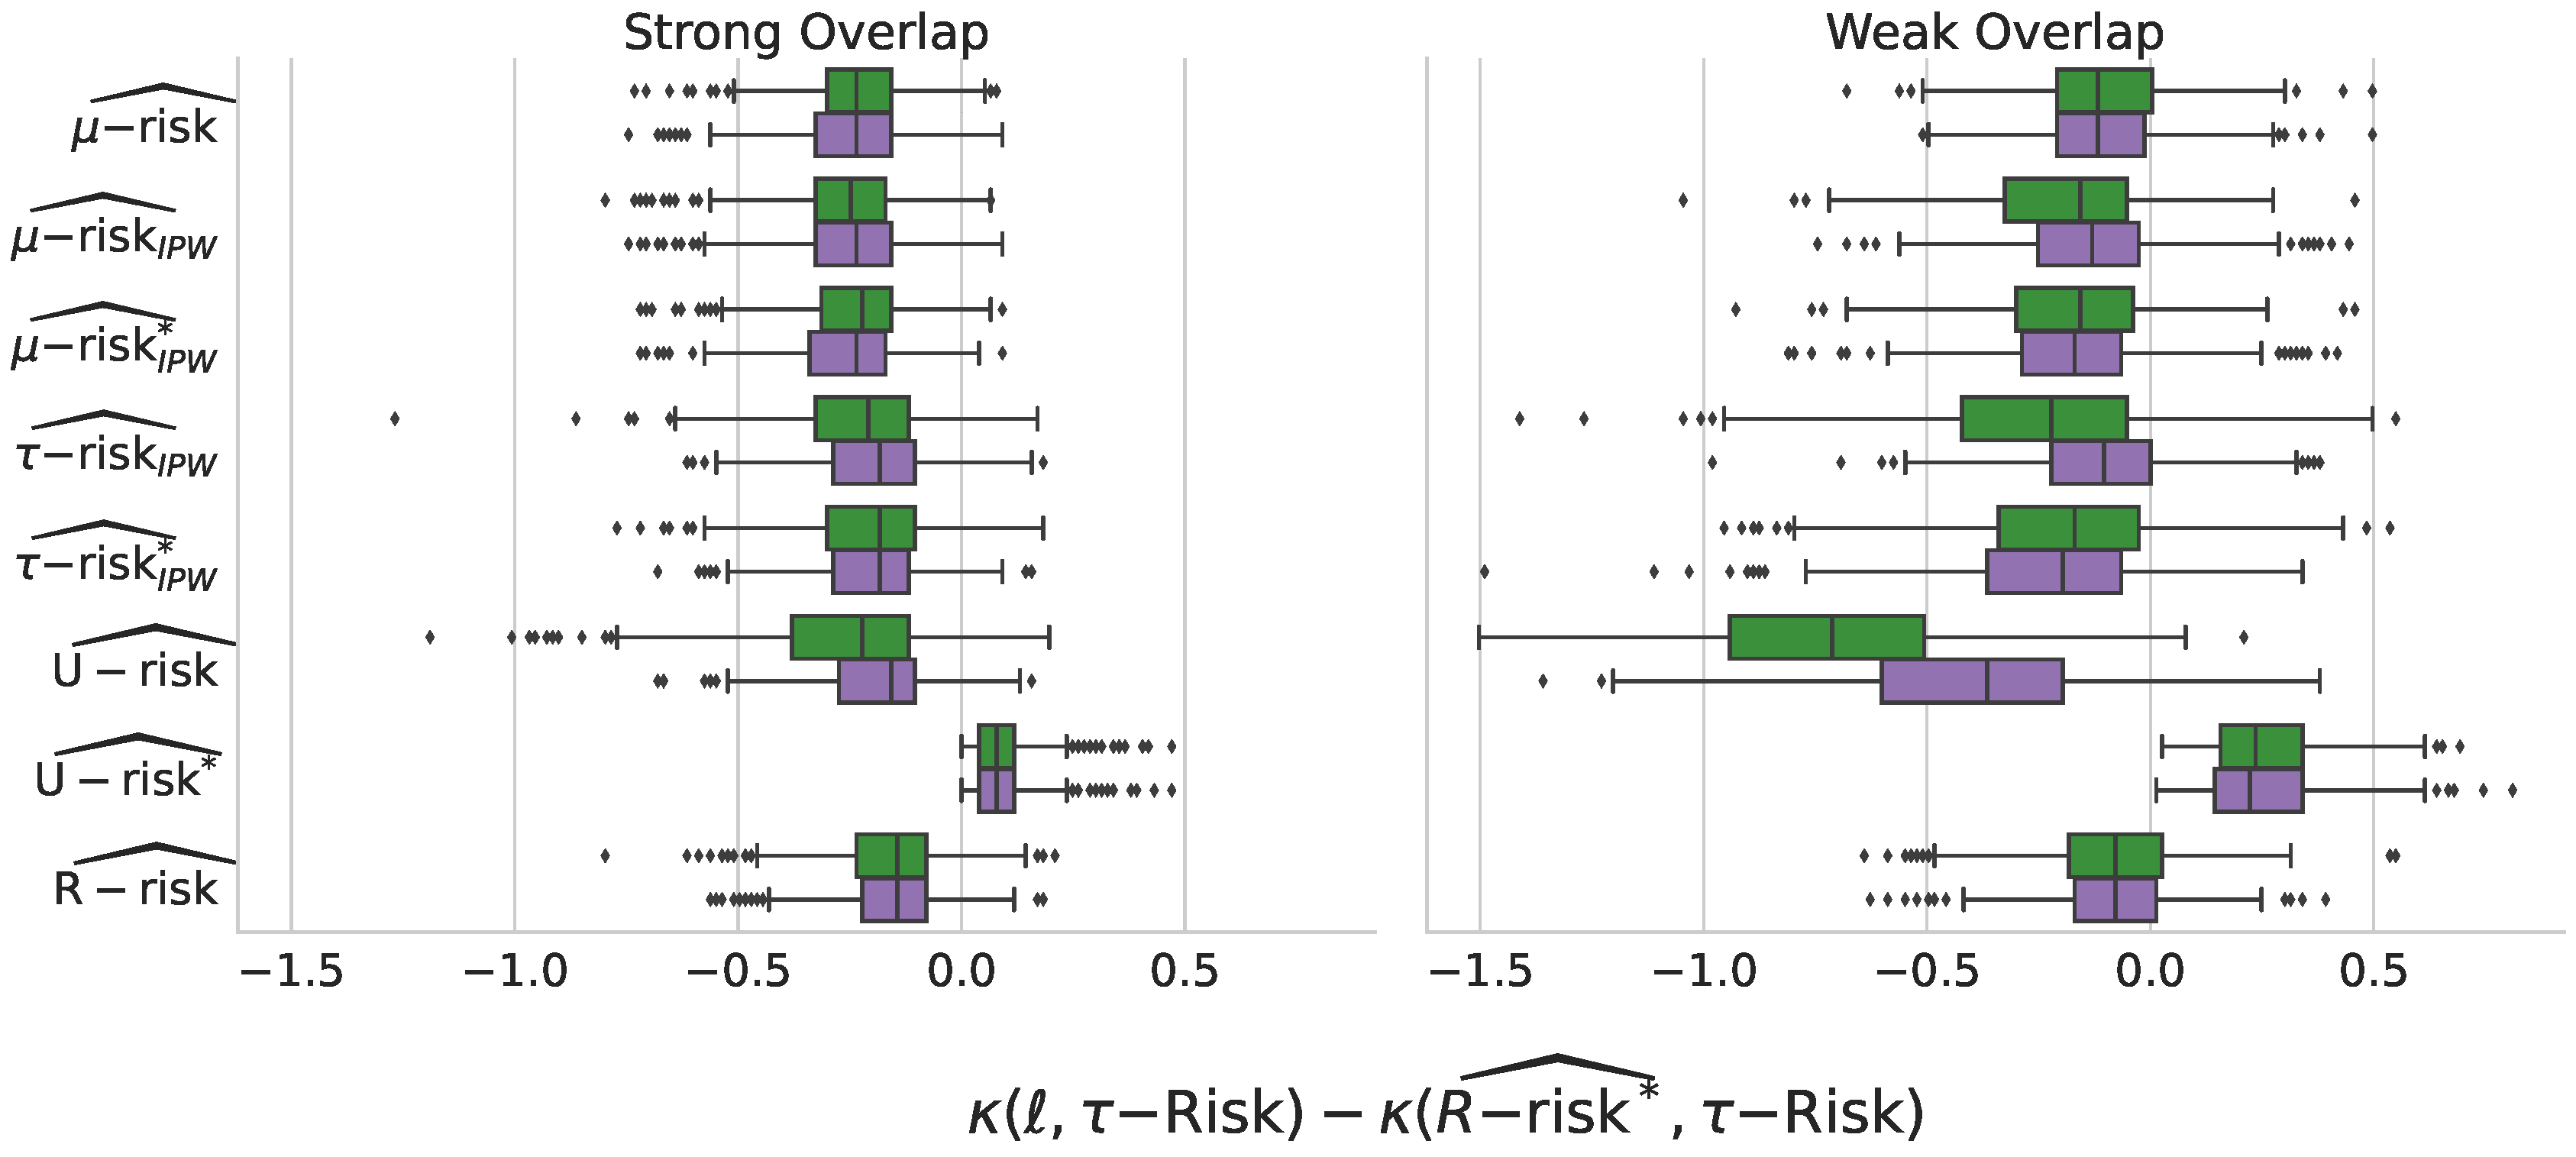
\includegraphics[width=1\textwidth]{img/chapter_5/_4_nuisance_models_Twinsdownsampled_N4794__ref_metric_oracle_r_risk_nuisance_models.pdf}
      \label{fig:experiments:nuisance_comparison:twins_ds}
    \end{subfigure}
    \hfill
    \begin{subfigure}[b]{0.49\textwidth}
      %\centering
      \caption{\textbf{Caussim}}
      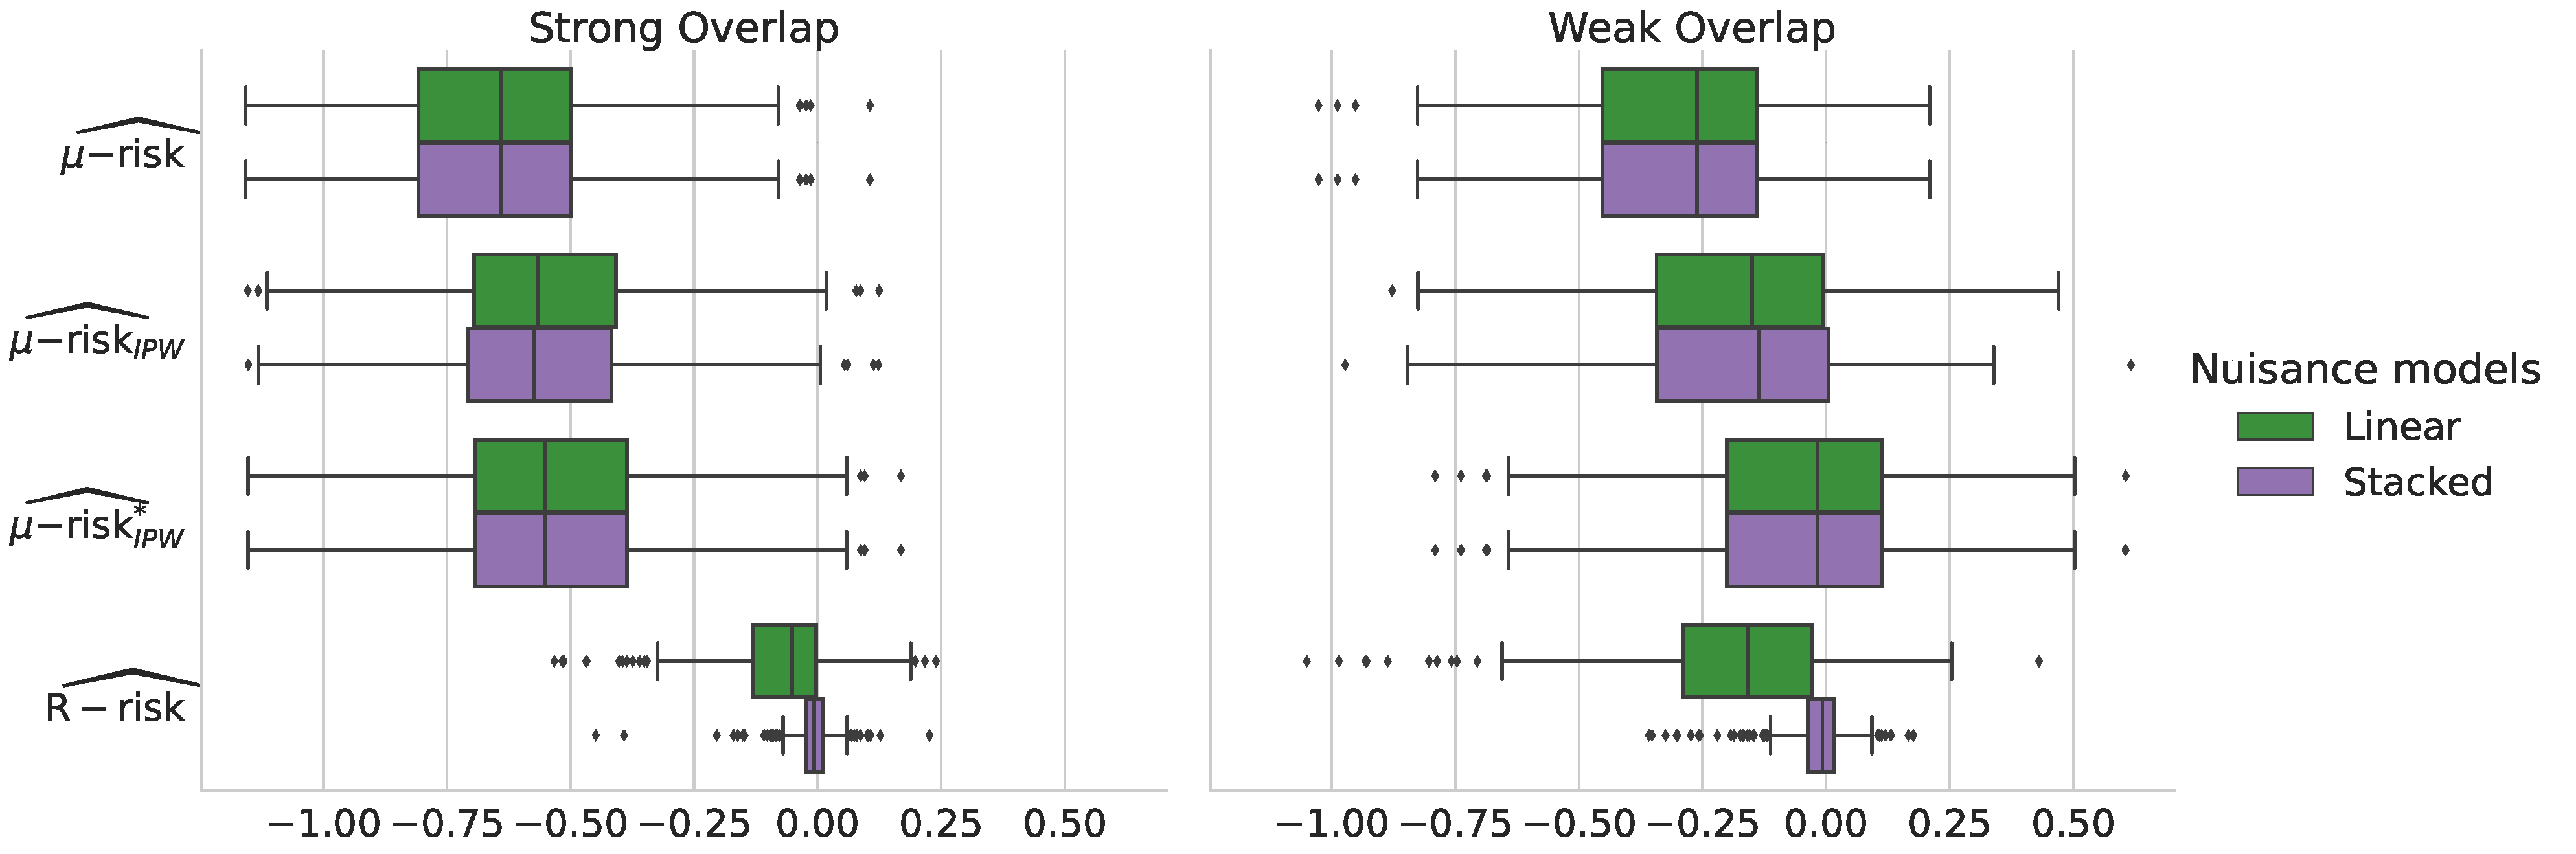
\includegraphics[width=1.15\textwidth]{img/chapter_5/_4_nuisance_models_Caussim_N5000__ref_metric_oracle_r_risk_nuisance_models.pdf}
      \label{fig:experiments:nuisance_comparison:caussim}
    \end{subfigure}
    \hfill
    \begin{subfigure}[b]{0.49\textwidth}
      \centering
      \caption{\textbf{ACIC 2016}}
      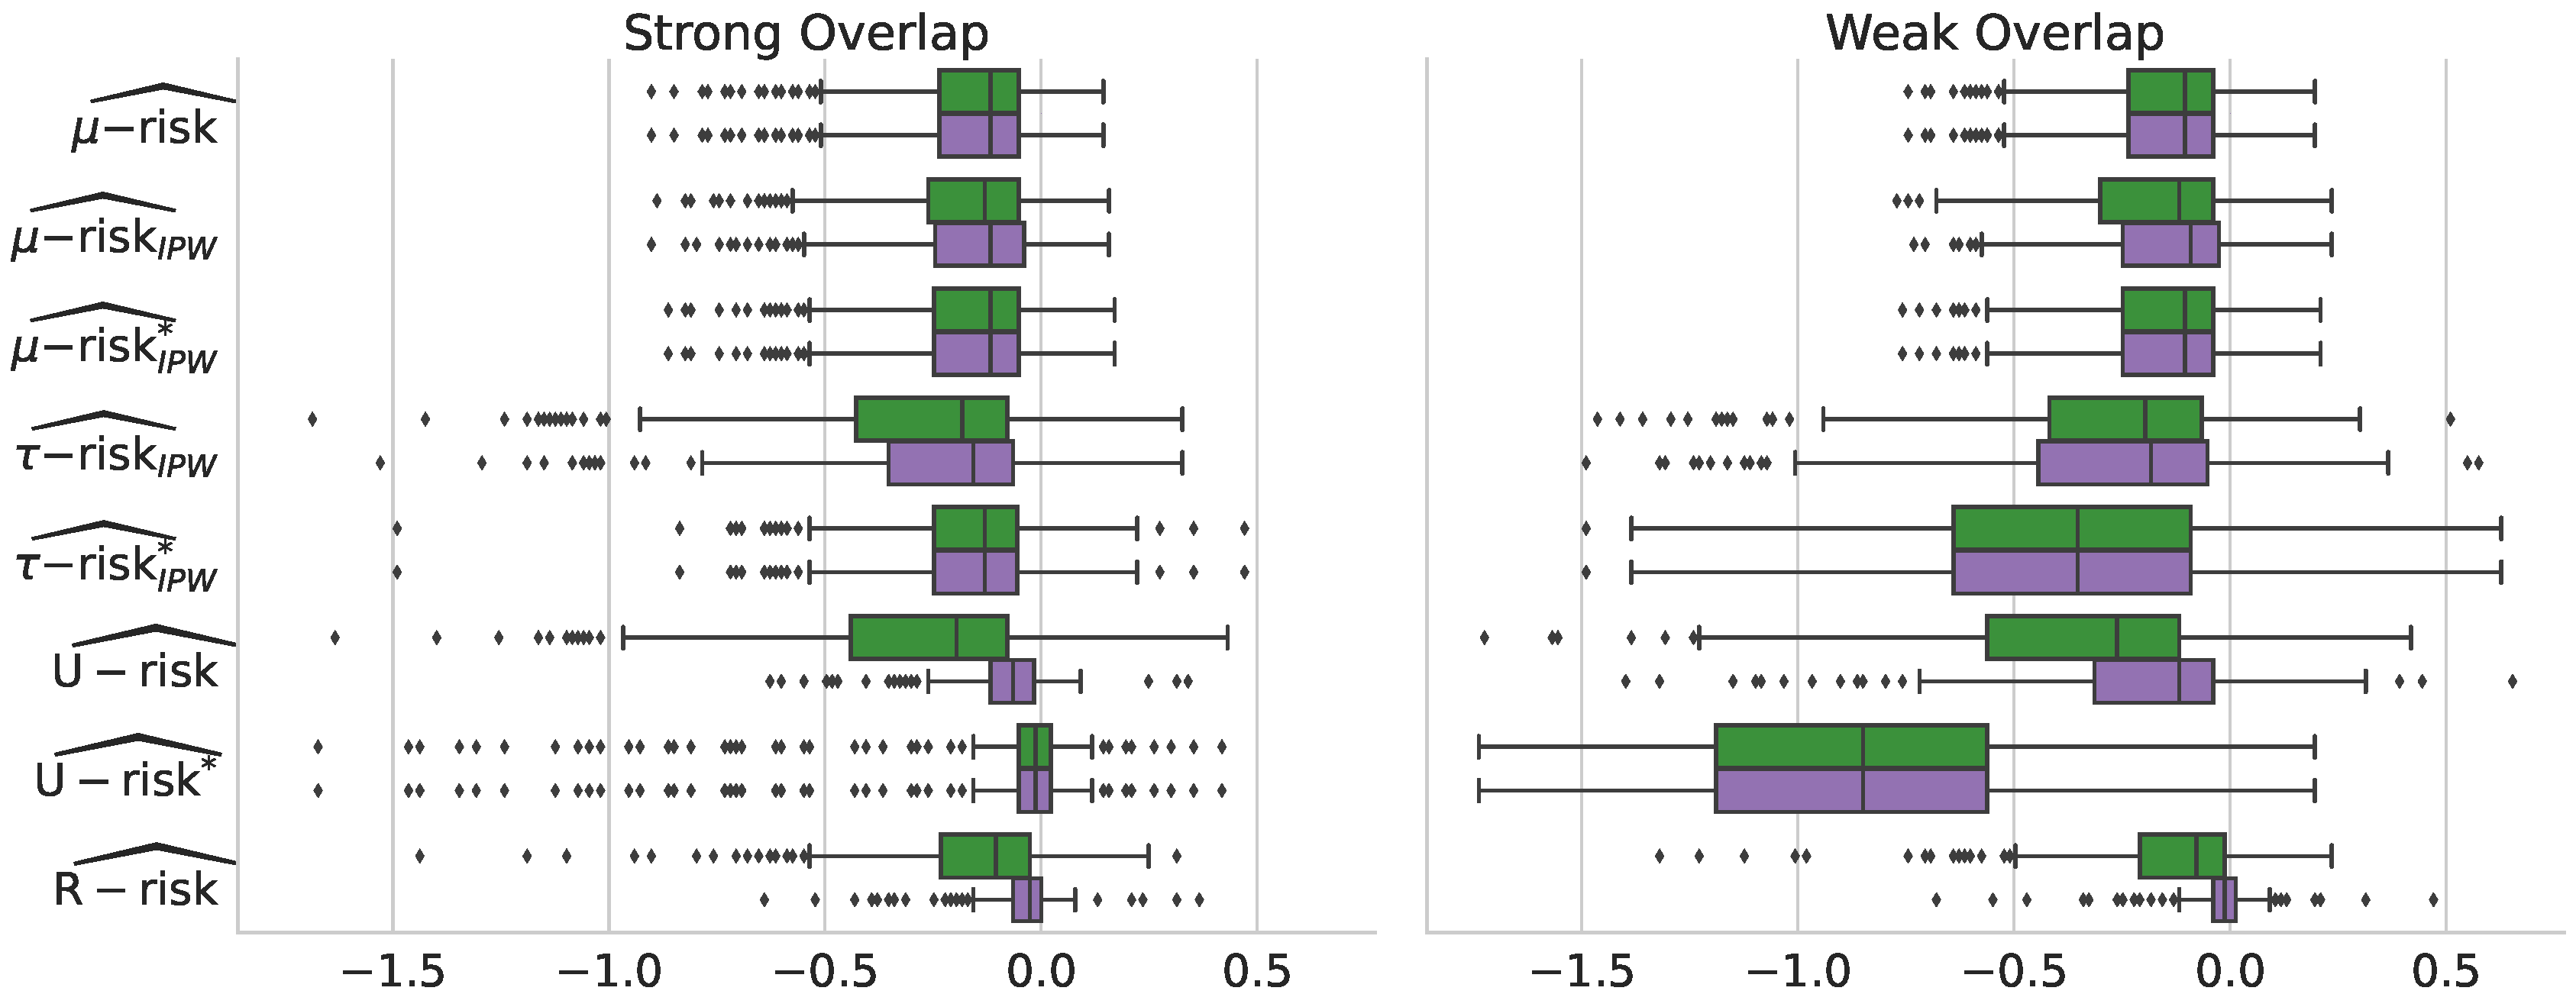
\includegraphics[width=1\textwidth]{img/chapter_5/_4_nuisance_models_ACIC2016_N4802__ref_metric_oracle_r_risk_nuisance_models.pdf}
      \label{fig:experiments:nuisance_comparison:acic_2016}
    \end{subfigure}
    \hfill
    \caption{Learning the nuisances with \textcolor{DarkOrchid}{stacked models} (linear and
      gradient boosting) is important for successful model selection with R-risk.
      For Twins dataset, there is no improvement for \textcolor{DarkOrchid}{stacked models} compared to
      \textcolor{ForestGreen}{linear models} because of the linearity of the propensity model.}\label
    {apd:fig:nuisances_comparison}
  \end{figure}

  \paragraph{Figure \ref{apd:fig:nuisances_comparison_twins} - Flexible models are performant in recovering nuisances even
    in linear setups}

  \begin{figure}
    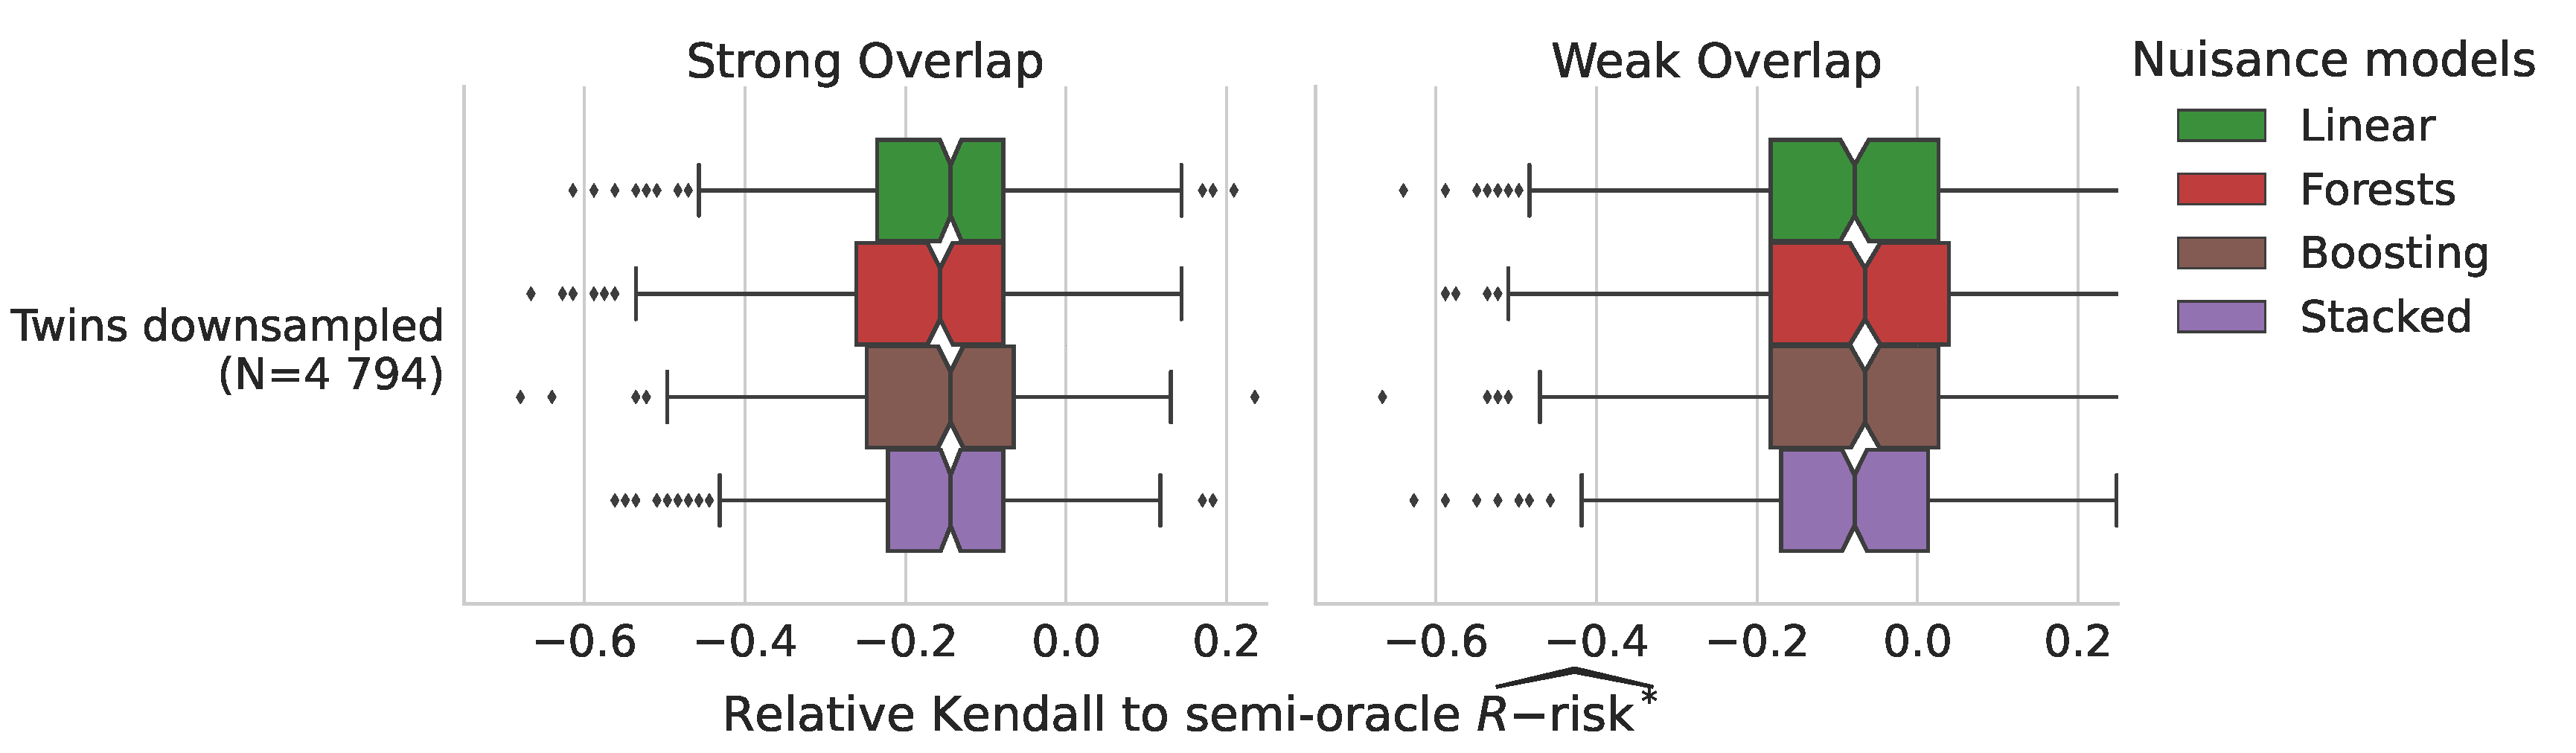
\includegraphics[width=\linewidth]{img/chapter_5/_4_nuisance_models_r_risk_only_twins_nuisances.pdf}
    \hfill
    \caption{\textbf{Flexible models are performant in recovering nuisances
        in the downsampled Twins dataset.} The propensity score is linear in this
      setup, making it particularly challenging for flexible models compared to
      linear methods.}\label{apd:fig:nuisances_comparison_twins}
  \end{figure}


  \paragraph{Selecting different seeds and parameters is crucial to draw
    conclucions}\label{{apd:results:seed_effect}}

  One strength of our study is the various number of different simulated and
  semi-simulated datasets. We are convinced that the usual practice of using only
  a small number of generation processes does not allow to draw statistically
  significant conclusions.

  Figure \ref{apd:results:fig:seed_effect} illustrate the dependence of the
  results on the generation process for caussim simulations. We highlighted the
  different trajectories induced by three different seeds for data generation and
  three different treatment ratio instead of 1000 different seeds. The result
  curves are relatively stable from one setup to another for $R{-risk}$, but vary
  strongly for $\mu\text{-risk}$ and $\mu\text{-risk}_{IPW}$.

  \begin{figure}
    \centering
    \caption{Kendall correlation coefficients for each causal metric. Each (color,
      shape) pair indicates a different (treatment ratio, seed) of the generation
      process.}\label {apd:results:fig:seed_effect}
    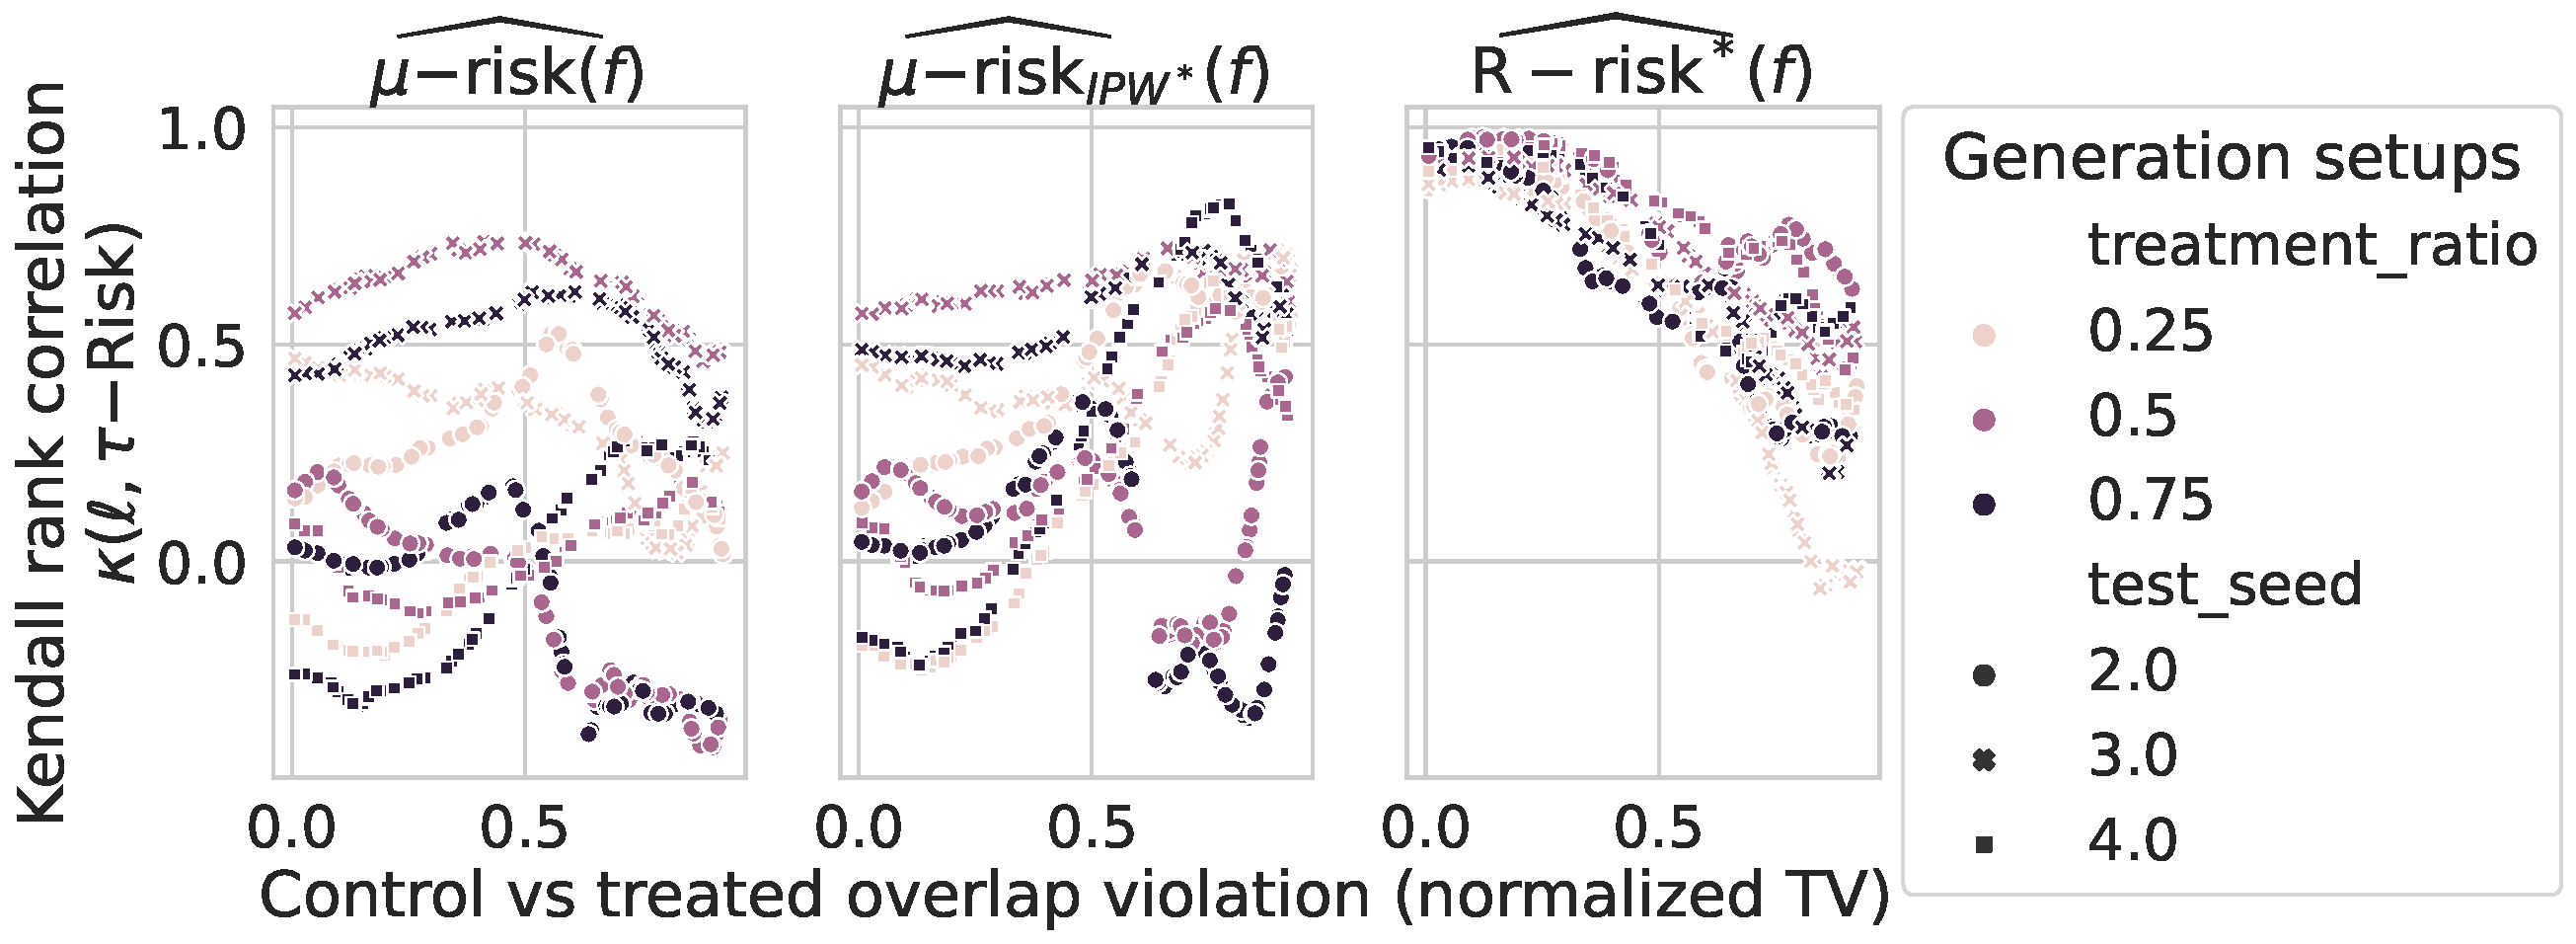
\includegraphics[width=\linewidth]{img/chapter_5/caussim_seed_effect.pdf}
  \end{figure}

  \FloatBarrier

  \section{Heterogeneity in practices for data split}\label{apd:results:k_fold_choices}

  Splitting the data is common when using machine learning for causal
  inference, but practices vary widely in terms of the fraction of data to
  allocate to train models, outcomes and nuisances, and to evaluate them.

  Before even model selection, data splitting is often required for
  estimation of the treatment effect, ATE or CATE, for instance to compute
  the nuisances required to optimize the outcome model (as the
  $R\text{-risk}$, definition \ref{def:r_risk}).
  %
  The most frequent choice is use 80\% of the data to fit the models,
  and 20\% to evaluate them.
  %
  For instance, for CATE estimation, the R-learner has been introduced using K-folds with K = 5
  and K = 10: 80\% of the data (4 folds) to train the nuisances and the remaining
  fold to minimize the corresponding R-loss \citep{nie_quasioracle_2017}.
  Yet, it has been implemented with K=5 in causallib
  \citep{causalevaluations} or K=3 in econML \citep{battocchi2019econml}.
  Likewise, for ATE estimation, \cite{chernozhukov_double_2018}
  introduce doubly-robust machine learning,
  recommending K=5 based on an empirical comparison K=2. However,
  subsequent works use doubly robust ML with varying choices
  of K: \cite{loiseau_external_2022} use K=3, \cite{gao_assessment_2021} use
  K=2. In the econML implementation, K is set to 3 \citep{battocchi2019econml}.
  \cite{naimi2021challenges} evaluate various machine-learning approaches
  --including R-learners-- using K=5 and 10, drawing inspiration from the
  TMLE literature which sets
  K=5 in the TMLE package \citep{tmle_package_2012}.

  Causal model selection has been much less discussed. The only study that
  we are aware of, \citet{schuler_comparison_2018}, use a different data
  split: a 2-folds train/test procedure,
  training the nuisances on the first half of the data, and using the
  second half to estimate the $R\text{-risk}$ and select the best treatment
  effect model.


  % \paragraph{Simulations: naive reweighting of the $R \text{-risk}$}

  % Applying a naive reweighting, $w(x, a)=\frac{1}{e(x)\big(1-e(x) \big )}$ to the
  % $R \text{-risk}$ to recover the $\tau \text{-risk}$ in the first part of
  % \ref{theory:prop:r_risk_rewrite} makes the residuals explode in case of noise as
  % shown in Figure \ref{apd:simu_noised}.


  % \begin{figure}[htbp]
  %   \centering
  %   \caption{Caussim simulations (500 repetitions):
  %   $R\text{-risk}_{IPW^*_{naive}}$ (in green) is exploding}\label
  %   {apd:simu_noised}
  %   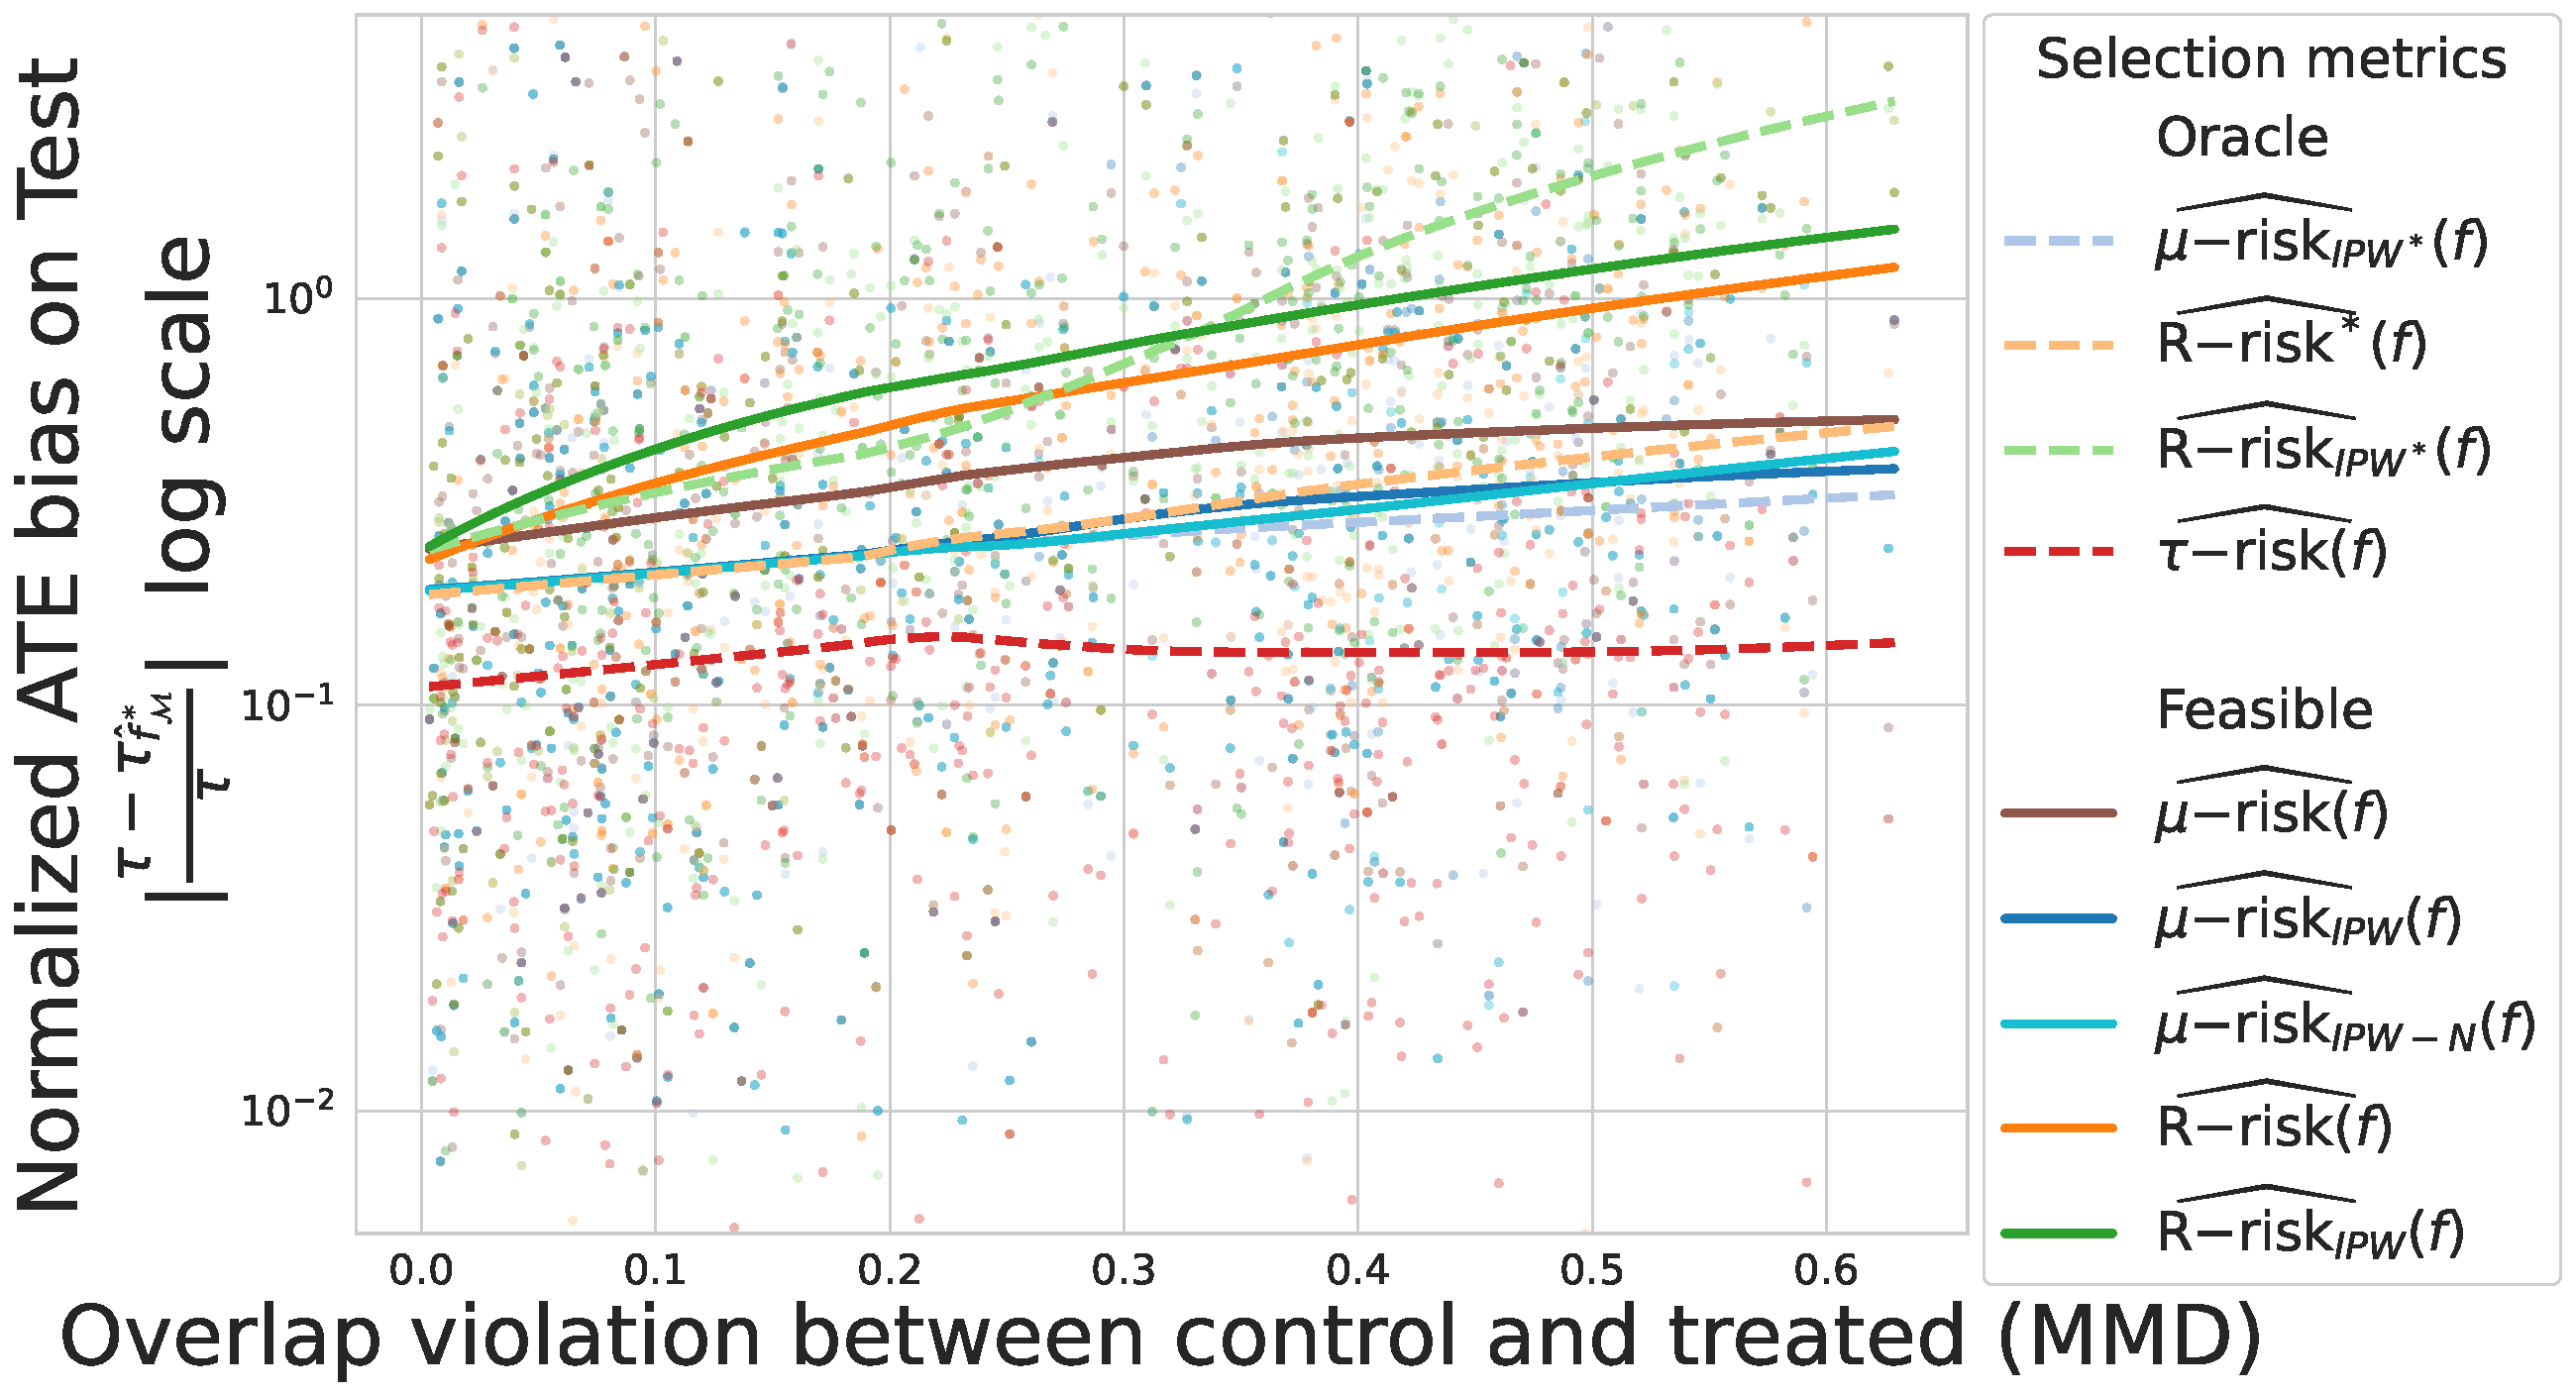
\includegraphics[width=0.7\linewidth]{img/chapter_5/noised_0.001_simu_best_normalized_abs_bias_ate_vs_mmd.pdf}
  % \end{figure}


\end{appendices}



%%%%%%%%%%%%%%%%%%%%%%%%%%%%%%%%%%%%%%%%%%%%%%%%%%%%%%%%%%%%%%%
% 4eme de couverture
\ifthispageodd{\newpage\thispagestyle{empty}\null\newpage}{}
\thispagestyle{empty}
\newgeometry{top=1.5cm, bottom=1.25cm, left=2cm, right=2cm}
\fontfamily{rm}\selectfont

\lhead{}
\rhead{}
\rfoot{}
\cfoot{}
\lfoot{}

\noindent
%*****************************************************
%***** LOGO DE L'ED À CHANGER IMPÉRATIVEMENT *********
%*****************************************************

\includegraphics[height=2.45cm]{img/EOBE}
\vspace{1cm}
%*****************************************************
\fontfamily{cmss}\fontseries{m}\selectfont

\small

\begin{mdframed}[linecolor=Prune,linewidth=1]

  \textbf{Titre:} Titre de la thèse en français


  \noindent \textbf{Mots clés:} Quelques mots-clé

  \vspace{-.5cm}
  \begin{multicols}{2}
    \noindent \textbf{Résumé:}Blabla
  \end{multicols}

\end{mdframed}

\begin{mdframed}[linecolor=Prune,linewidth=1]

  \textbf{Title:} Thesis title in English

  \noindent \textbf{Keywords:} Some keywords

  \begin{multicols}{2}
    \noindent \textbf{Abstract:} Blabla
  \end{multicols}
\end{mdframed}

%************************************
\vspace{\fill} % ALIGNER EN BAS DE PAGE
%************************************

\noindent
\color{Prune} \footnotesize Maison du doctorat de Université Paris-Saclay\\
2$^{\mathrm{e}}$ étage, aile ouest, École normale supérieure Paris-Saclay\\
4 avenue des Sciencs\\
91190 Gif-sur-Yvette, France
\end{document}
